\clearpage
%\begin{savequote}[8cm]
%\textlatin{Neque porro quisquam est qui dolorem ipsum quia dolor sit amet, consectetur, adipisci velit...}
%
%There is no one who loves pain itself, who seeks after it and wants to have it, simply because it is pain...
%  \qauthor{--- Cicero's \textit{de Finibus Bonorum et Malorum}}
%\end{savequote}

\chapter{\label{ch:4-selection}Selection and mass parameterisation of \btodkst decays} 

%\minitoc

\section{Selection of \btodkst candidates}
\label{sec:selection}

In this chapter, the reconstruction and selection procedure for the signal mode \decay{\Bm}{\D\Kstarm}(\KS\pim) is described, where the particles in brackets refers to the decay products of the preceding particle. The symbol \D refers to a superposition of \Dz and \Dzb mesons. In this thesis the \Dz meson final states investigated are \Km\pip, \Kp\Km, \pip\pim, \Kp\pim, \Km\pip\pim\pip, \pip\pim\pip\pim, and \Kp\pim\pip\pim. The \pim from the \Kstarm decay is referred to as the bachelor particle. The selection is developed for the favoured \kpi mode and then applied with minor alterations to the other \D decay modes. The data analysed correspond to 1~\invfb and 2~\invfb of $pp$ collisions at $\sqrt{s} = 7~\tev \text{ and } 8~\tev$ collected in 2011 and 2012 (referred to as Run 1), and 1.8~\invfb at $\sqrt{s} = 13~\tev$ collected in 2015 and 2016 (referred to as Run 2).

\subsection{Reconstruction and trigger requirements}
\label{sec:selection:strippingandtrigger}

\decay{\Bm}{\D\Kstarm}(\KS\pim) decays are reconstructed offline and stored in a centrally produced dataset in a stage known as stripping, described in \sect\ref{sec:detector:stripping}. At this point of the data-processing chain some loose requirements have been made in order to reduce the \dataset to a reasonable size for storage. However, the amount of combinatorial background, originating from reconstructing random pion and kaon tracks to form fake \Bm, \Dz, \KS or \Kstarm candidates, is still very high. Therefore further offline selection is applied to candidates passing the stripping and trigger requirements in order to reduce the level of combinatorial background, as well as to target specific peaking backgrounds.

The decay is reconstructed starting from the final state particles, and proceeding up the decay chain. In this case, the reconstruction proceeds with \decay{\KS}{\pim\pim}, \decay{\Kstarm}{\KS\pim}, \decay{\Dz}{\Km\pip} and finally \decay{\Bm}{\D\Kstarm}; at each stage a fit is performed to the parent candidate.

The \KS meson is reconstructed through its decay to two charged pions. Reconstructed tracks can be classified into different types as described in \sect\ref{sec:detector:tracks}. If the pions from the \KS decay leave sufficient hits in the \velo to be included in the track reconstruction they are called long tracks and the reconstructed \KS meson is referred to as LL. Due to the high boost from the $pp$ collision many \KS particles decay outside the \velo. If the pions from the \KS decay do not leave sufficient hits in the \velo, they are called downstream tracks and the reconstructed \KS meson is referred to as DD, with the first hits being recorded in the TT, which typically results in poorer mass resolution. The LL \KS mesons tend to have higher combinatorial background levels as there are many more tracks in the \velo to be misreconstructed compared to further downstream. Due to these differences, the \KS reconstruction types, LL and DD, are treated as separate data samples and a slightly different selection is applied to each.

The \KS candidates are required to have a reconstructed mass within 15~\mevcc of the known mass for LL \KS candidates and within 20~\mevcc for DD \KS candidates. The \KS candidate is also required to have a good quality vertex that is well separated from the primary vertex. The \Kstarm candidate is formed from a reconstructed \KS candidate and a \pim candidate, and is required to have a reconstructed mass within 75~\mevcc of the known \Kstarm mass. Similarly the \Dz candidate is reconstructed from the relevant kaon and pion candidates, \eg~in the case of \kpi, a \Km and \pip are reconstructed to form a \Dz candidate, which is required to form a good quality vertex, with a reconstructed mass within 25~\mevcc of the known \Dz mass. The \Bm candidate is reconstructed from a \Dz and a \Kstarm candidate forming a good quality vertex. The resulting reconstructed \Bm candidate is required to have a mass in the range 4750 - 5800 \mevcc and a \chisqip $<$ 25, where \chisqip is the difference in the vertex fit \chisq of the PV with and without the particle under consideration. Additionally, there are loose $p$ and \pt threshold requirements on all charged tracks.

The trigger decision for each candidate is categorised as {\tt TOS} (Trigger On Signal) if the particles associated with the signal candidate triggered the event or {\tt TIS} (Trigger Independent of Signal) if other particles produced in the $pp$ interaction, that are not associated with the signal candidate, triggered the event. At the hardware trigger, the \Bm candidates are required to satisfy {\tt L0Hadron TOS} or {\tt L0Global TIS}. At the software trigger level, \Bm candidates are required to satisfy {\tt Hlt2TopoNBodyBBDT TOS}, where $N = 2,3 \text{ or } 4$. These trigger classifications are described in \sect\ref{sec:detector:trigger}.

This analysis uses variables constructed after the entire decay chain has been refitted for all the reconstructed tracks in the decay for each \Bm candidate passing the stripping requirements, with one or more constraints imposed~\cite{Hulsbergen:2005pu}. During this refit, the best fit value of the four-momenta for each particle is found under the given constraints. This procedure improves the resolution of the \Bm mass peak compared to the original variables constructed without the refit performed. The \Bm mass used in this analysis is constructed for each \Bm candidate by fitting the tracks in the decay with requirements that the \Dz and \KS mass are constrained to their known values and the \Bm momentum vector direction is constrained to be parallel to the vector joining the primary vertex (PV) to the \Bm decay vertex.

The offline selection involves imposing requirements on individual variables, such as the reconstructed masses of the intermediate meson states, as well as using a multivariate classifier, and particle identification requirements. The requirements on the masses of the intermediate states reduce the probability of the sample containing \Dz, \KS or \Kstar candidates that do not correspond to a true \Dz, \KS or \Kstar meson state. However, the requirements cannot be too close to the true meson mass as this would result in the removal of a significant proportion of the signal. The signal efficiencies of the \Dz, \KS and \Kstar mass requirements, shown graphically in \fig\ref{masscuts}, are 96\%, 98\% and 82\% respectively. 

\begin{figure}
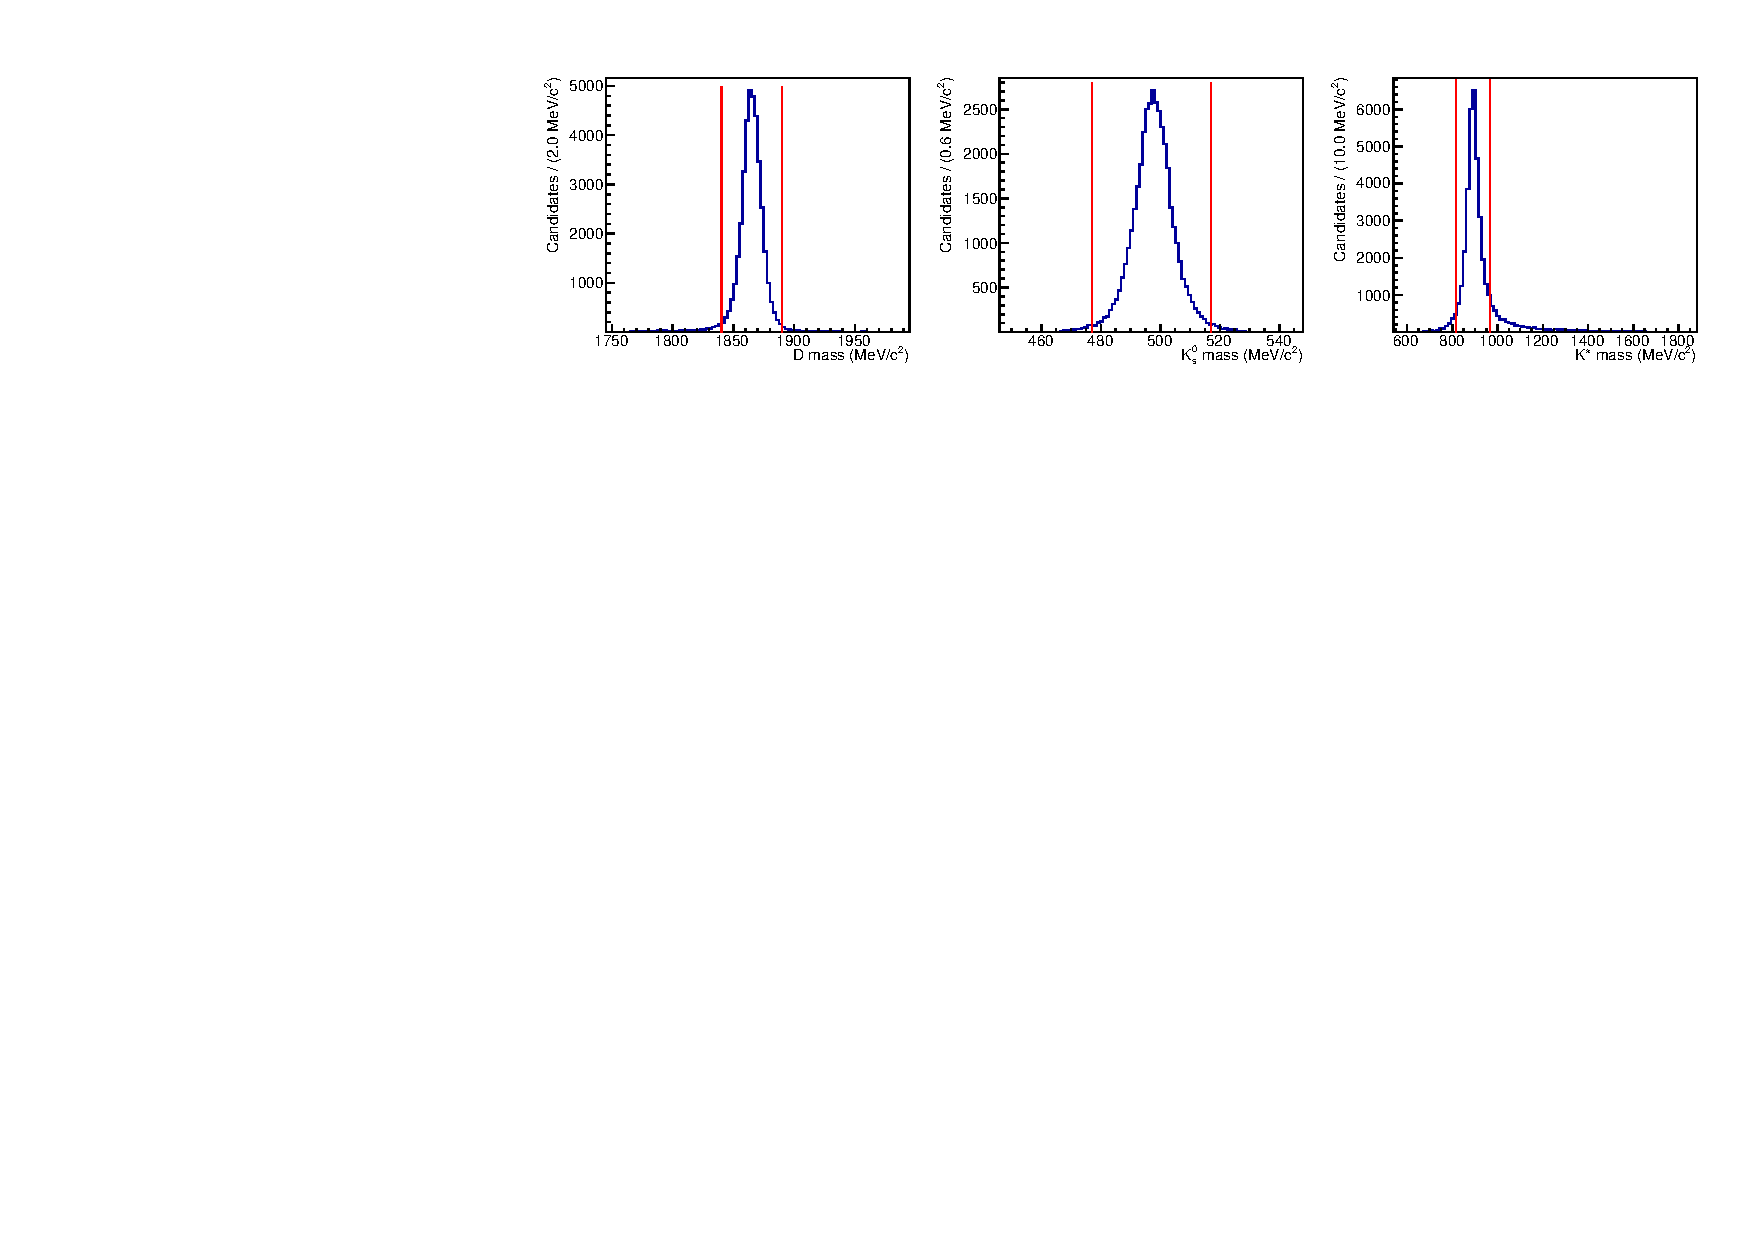
\includegraphics[width=\linewidth]{figures/selection/massDistDD_MC.pdf}
\put(-380,80) {(a)}
\put(-245,80) {(b)}
\put(-110,80) {(c)}
\caption{Distributions of the reconstructed masses from a simulated sample of \kpi DD events for (a) \Dz, (b) \KS, and (c) \Kstar candidates. The red lines represent the regions accepted as signal in the selection.}
\label{masscuts}
\end{figure}

After the selection described in this section has been applied, the resulting refitted \Bm mass distribution is shown for \runtwo data in \fig\ref{fig:BmassbeforeBDT}. The signal \Bm mass peak can be clearly observed, however, in order to make accurate measurements of the signal yield in each of the \Dz modes, it is necessary to significantly reduce the combinatorial background while retaining signal events. This requires more sophisticated classification techniques. Additionally, specific backgrounds must be reduced, and particle identification requirements must be made to reduce the fraction of misidentified particles.

\begin{figure}
\centering
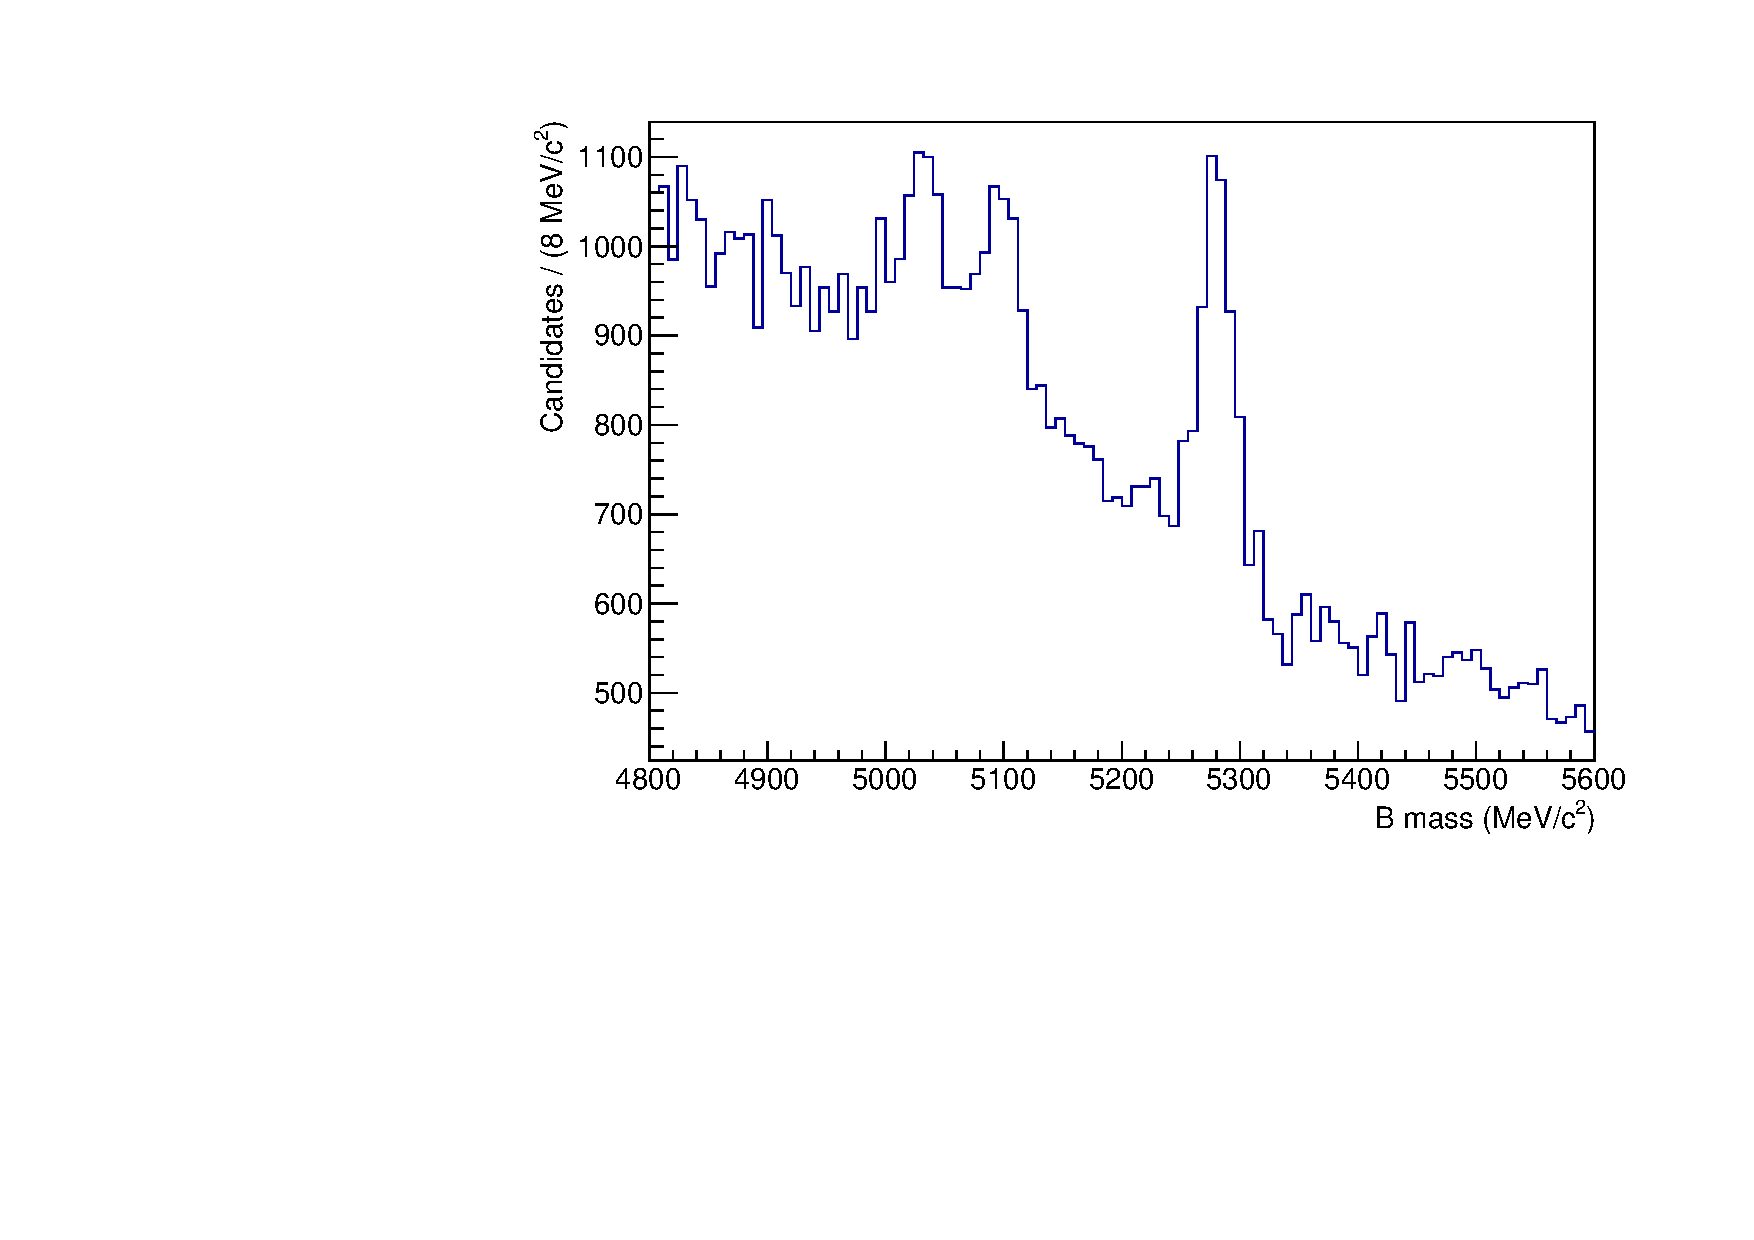
\includegraphics[width=0.6\linewidth]{figures/selection/DataDD_KPi_beforeBDT.pdf}
\caption{The refitted \Bm mass distribution for \kpi DD candidates in \runtwo after the stripping and mass requirements on the intermediate states. The \Bm signal peak can be seen at the known \Bm mass (5279 \mevcc) and the peaks at lower reconstructed \Bm mass are discussed in \sect\ref{sec:backgrounds:partreco}.}
\label{fig:BmassbeforeBDT}
\end{figure}


\subsection{Particle identification requirements}
\label{sec:selection:pid}

The selection requirements are almost identical for each of the different \Dz decay modes, therefore, in order to distinguish the different modes it is essential to apply PID selection that efficiently distinguishes between pions and kaons. For both the two- and four-body \Dz decays, the suppressed \Dz decay modes may have contamination from the most favoured mode, with one or more of the \Dz daughter particles  incorrectly identified. These backgrounds are called crossfeed backgrounds. The ratios of branching fractions for two- and four-body \Dz decay modes are given in \tab\ref{BFdmodes}. The contamination of the most favoured mode is considered as it has the largest branching fraction and therefore would have the largest crossfeed contribution in the disfavoured \Dz modes.

\begin{table}[h]
\centering
\begin{tabular}{c|c}
Mode & Branching fraction ratio \\
\hline
\kpi & 1 \\
\kk & 0.10 \\
\pipi & 0.036 \\
\pik & 0.0036 \\
\hline
\hline
\kpipipi & 1 \\
\pipipipi & 0.092 \\
\pikpipi & 0.0036 
\end{tabular}
\caption{Branching fractions of the different \Dz decay modes relative to the favoured \kpi mode~\cite{PDG2016}. The ratio given for \pikpipi is approximate as the branching fraction has not been measured. Here it has been estimated to be the same as the ratio between the two-body favoured and suppressed modes as $r_D^{K\pi} \approx r_D^{K3\pi}$.}
\label{BFdmodes}
\end{table} 

Consider first the two-body \Dz decay modes. The suppressed modes may all contain a background from the favoured \kpi mode, where one or more of the \Dz daughters has been incorrectly identified. Examples can be seen in \fig\ref{fig:crossfeed}, which shows the \Dz mass spectrum for the \kk and \pipi data samples both without and with PID requirements applied. \Fig\ref{crossfeedkk} (left) contains a \Dz mass peak, but to the right of this there is a second, larger peak, which corresponds to the crossfeed from \kpi events. This peak occurs at higher reconstructed \Dz mass due to the misidentification of the pion as a kaon, which is then added to the invariant mass sum. However, the low mass tail of this large distribution enters into the selected region of \Dz mass, with the selected region illustrated by the red lines. By applying PID requirements on the two \Dz daughter kaons, this crossfeed background can be reduced such that there is negligible contribution within the \Dz mass region, as shown in \fig\ref{crossfeedkk} (right). 

The same effect is seen in the \pipi mode, illustrated in \fig\ref{crossfeedpipi}. In this case, the crossfeed peak is lower in invariant mass, as a pion is misidentified as a kaon. Also, the crossfeed peak in \fig\ref{crossfeedpipi} (left) is significantly higher than in \fig\ref{crossfeedkk} (left), due to a much lower \decay{\Dz}{\pip\pim} branching fraction, as seen in \tab\ref{BFdmodes}.

\begin{figure}
\subfloat[\kk]{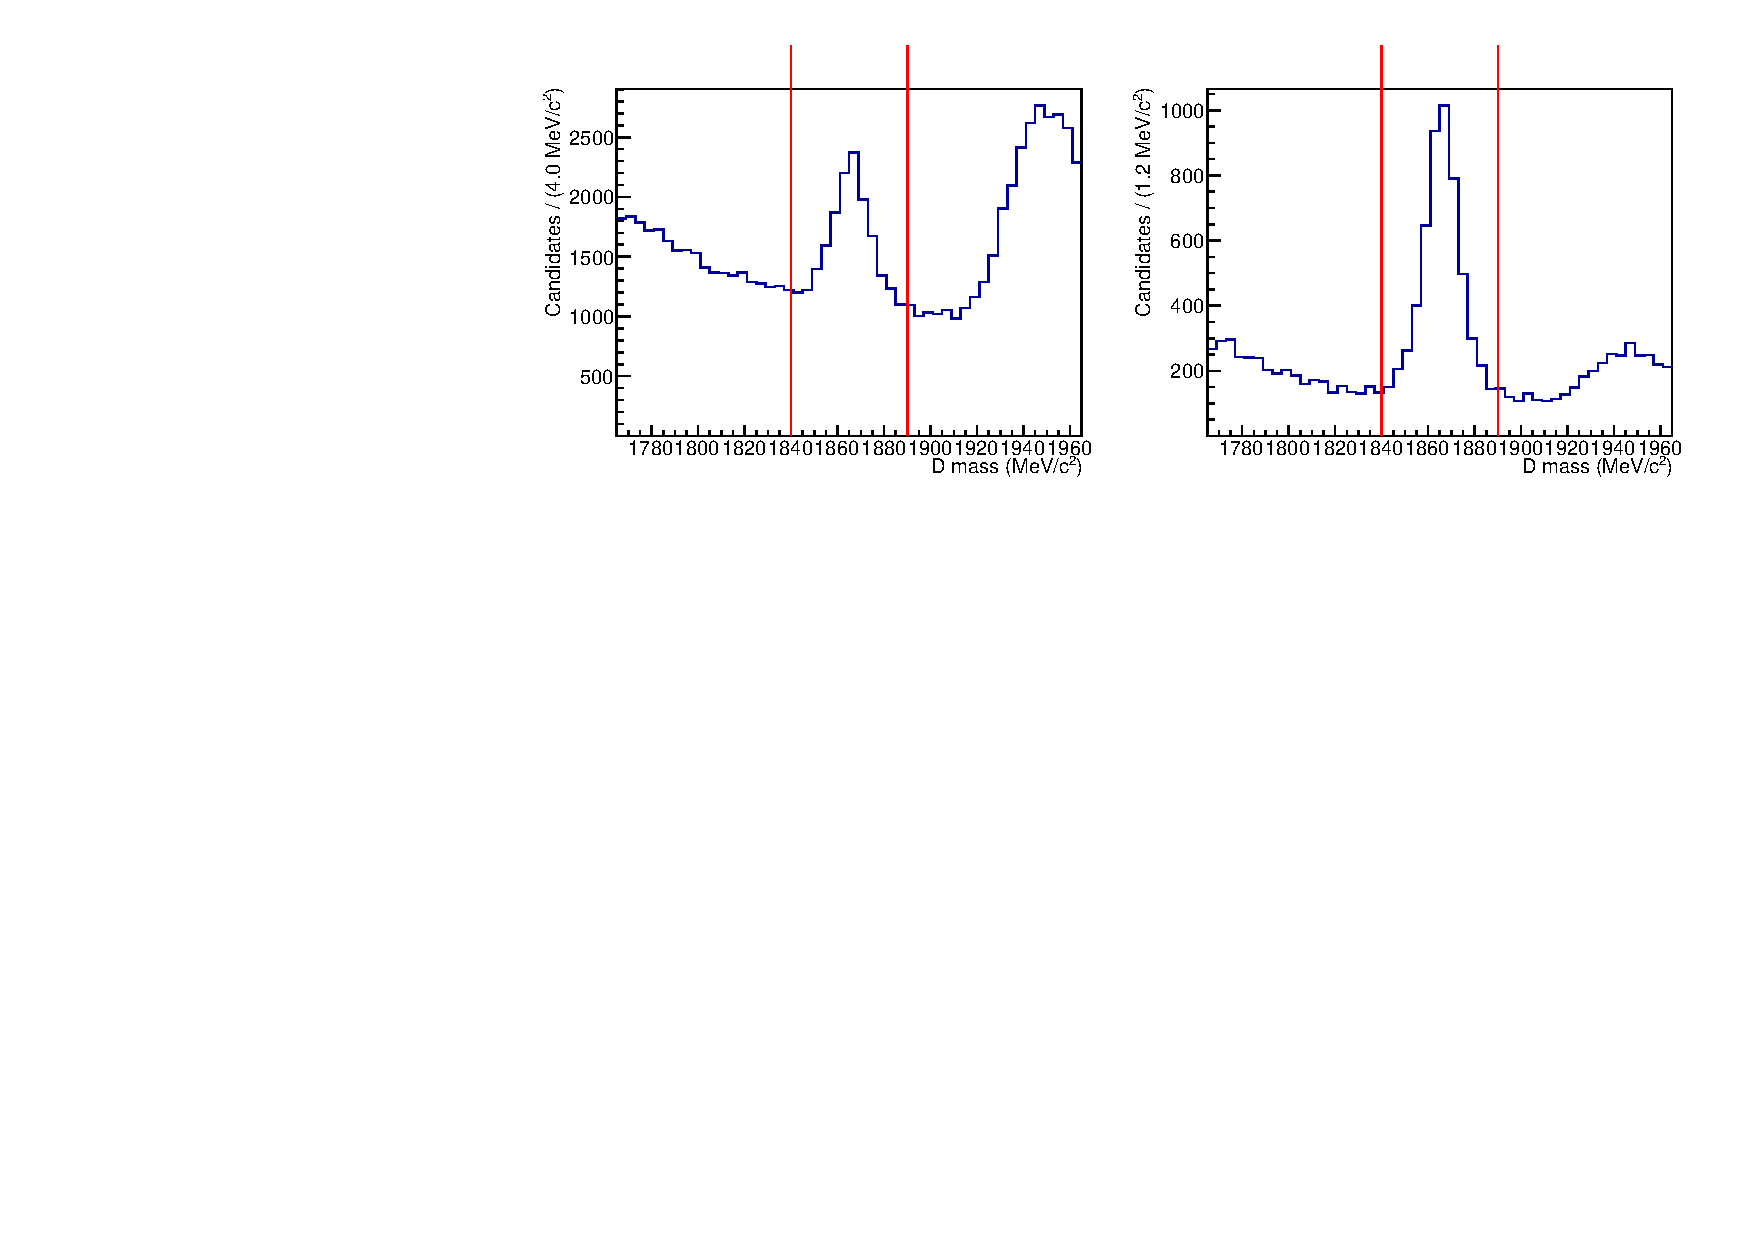
\includegraphics[width=\linewidth]{figures/selection/Dmass_pidcrossfeed_KK.pdf} \label{crossfeedkk}}
\hfill
\subfloat[\pipi]{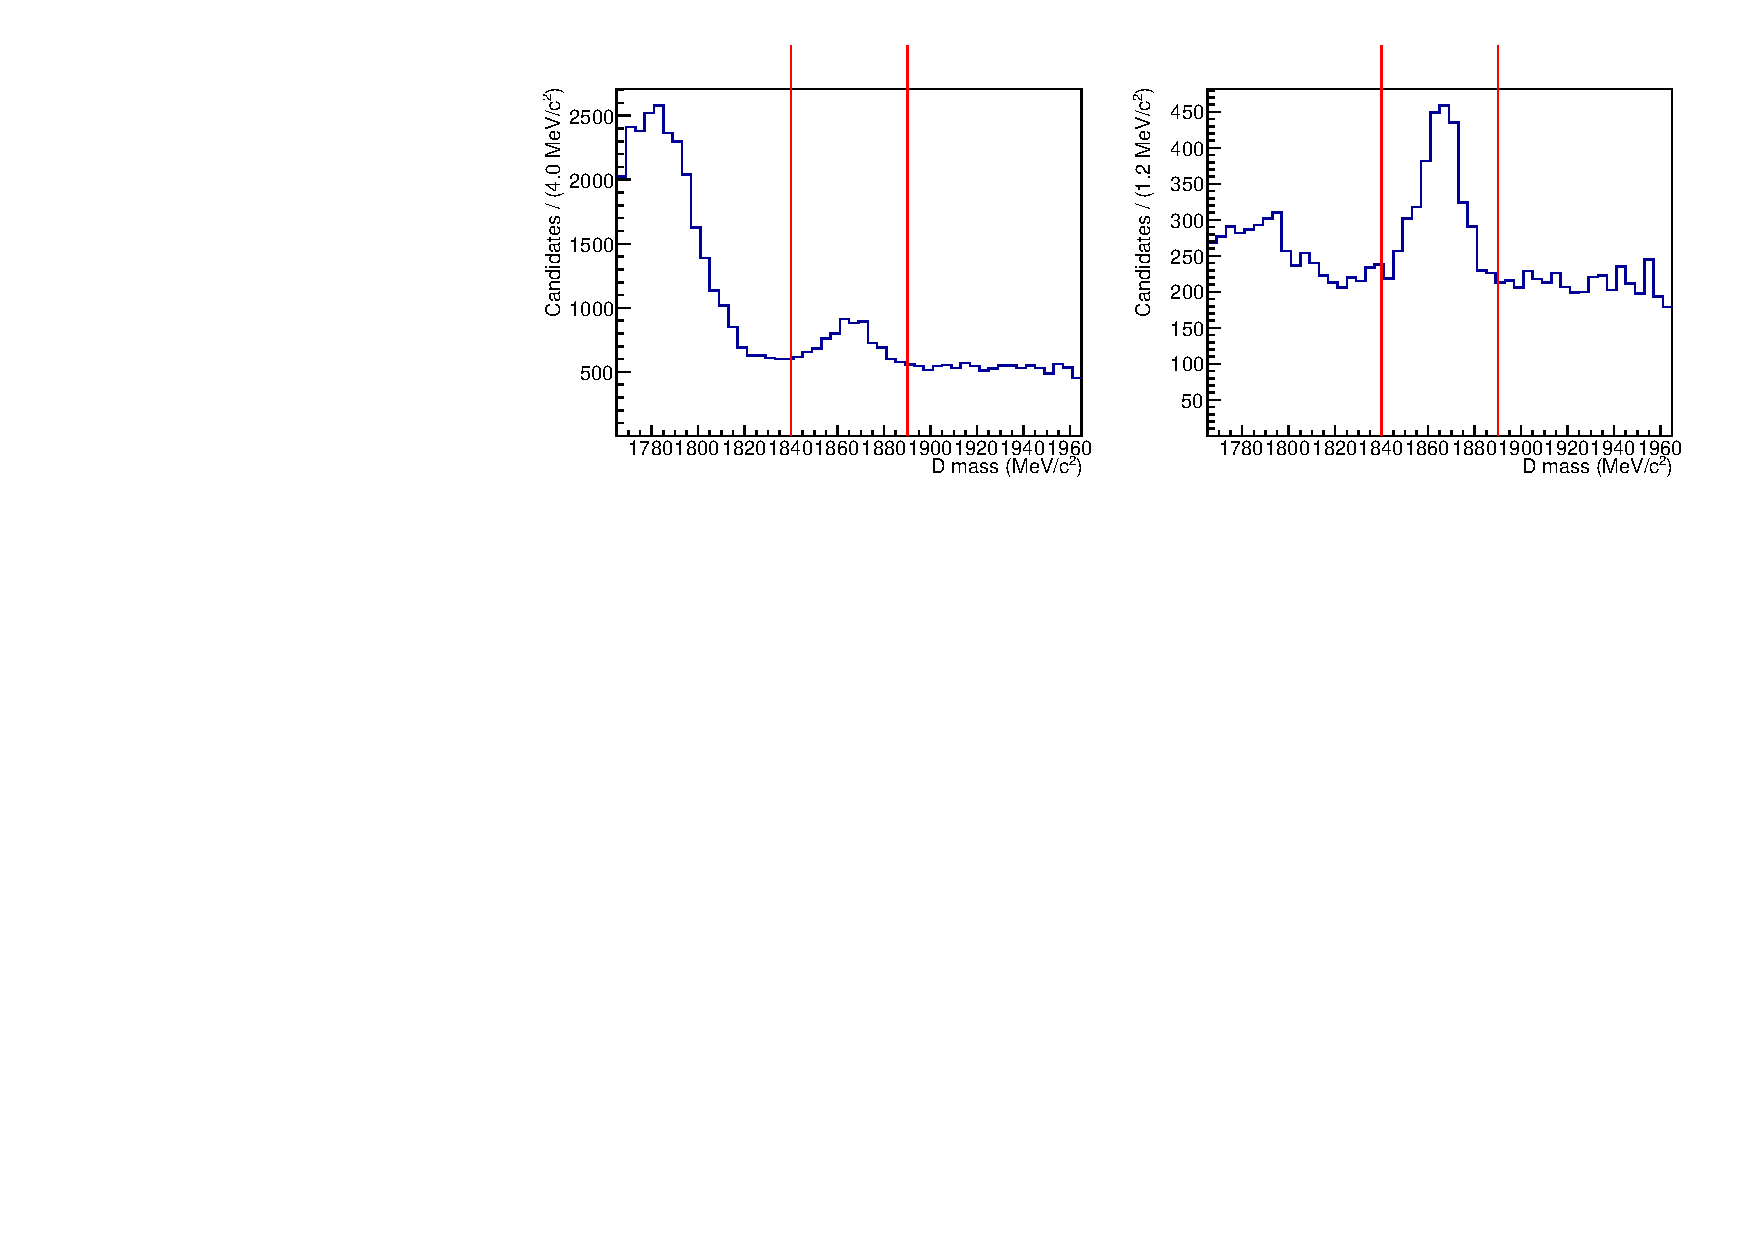
\includegraphics[width=\linewidth]{figures/selection/Dmass_pidcrossfeed_PiPi.pdf} \label{crossfeedpipi}}
\caption{Reconstructed \Dz mass distributions after a preliminary selection with no PID selection (left) and PID selection on the \Dz daughters (right), for (a) \kk and (b) \pipi. The red lines indicate the position of the \Dz mass requirement in the selection; events that fall between the red lines are retained as signal events.}
\label{fig:crossfeed}
\end{figure}

The PID requirements on the daughters of the \Dz meson are designed so that no \decay{\Dz}{hh'} candidate can appear in more than one category with a change in mass hypothesis. For the two-body \Dz modes the requirements on the \Dz daughters are: kaons must satisfy DLLK $>$ 2 and pions must satisfy DLLK $<$ -2, where DLLK is defined in \sect\ref{sec:detector:rich}. These requirements have a signal efficiency of 80\% on the \kpi mode, and the probability of incorrect identification of both the kaon and the pion is 0.13\%, ensuring negligible crossfeed background. Crossfeed from \kpi events entering the \pik mass spectrum would require both \Dz daughters to be misidentified, therefore the resulting reconstructed \Dz mass would not be shifted overall, so fall under the signal \Dz mass peak. This is called the doubly misidentified crossfeed background. In order to reduce this background to negligible levels, the PID requirement cannot be tightened further as this would result in an unacceptable loss of signal. Therefore, a further requirement is applied to the \pik mode, discussed in detail in \sect\ref{sec:backgrounds:crossfeed}.

The same arguments for the two-body \Dz decays modes also apply to the four-body modes. Crossfeed backgrounds may occur in the suppressed \Dz modes from misidentified \kpipipi events. Tight PID requirements must be placed on the \Dz daughters in order to reduce these crossfeed backgrounds to negligible levels. For the \decay{\Dz}{\Kmp\pipm\pimp\pipm} modes, e.g. \decay{\Dz}{\Km\pip\pim\pip}, the \Km must satisfy DLLK $>$ 2 and both \pip must satisfy DLLK $<$ -2; no PID requirement is applied for the \pim because the background \decay{\Dz}{\Kp\Km\Kp\pim} has a very low branching fraction~\cite{PDG2016}. These requirements have a signal efficiency of 74\% on the \kpipipi mode, and the probability of incorrect identification of both the \Km and the \pip is 0.10\%. For the \decay{\Dz}{\pip\pim\pip\pim} mode, the two pions that are of the same charge as the bachelor particle (the pion originating directly from the \Kstarm decay) must satisfy DLLK $<$ -2. No PID requirements are placed on the other pions because these decays correspond to Cabibbo suppressed backgrounds, and therefore are insignificant. The doubly misidentified crossfeed background from \kpipipi events in the \pikpipi mode must be investigated further in order to reduce it to negligible levels, as detailed in \sect\ref{sec:backgrounds:crossfeed}.

In addition to the correct identification of the \Dz daughters, it is also necessary to consider possible misidentification of the bachelor pion. A PID requirement is made on this bachelor pion to lower the combinatorial background and reduce the \decay{\Bm}{\D\KS\Km} background to negligible levels. The \decay{\Bm}{\D\KS\Km} background is discussed in more detail in \sect\ref{sec:backgrounds:b2dkks}. For all \Dz decay modes, the bachelor pion is required to satisfy DLLK $<$ 4. This requirements has a signal efficiency of 96.4\% when applied to the \kpi mode, and the probability of misidentification of the bachelor pion is 7.9\%. No PID requirements are placed on the \KS daughters as this is not necessary due to the high purity of the \KS meson, described in \sect\ref{sec:backgrounds:contamination}. The efficiencies of the PID requirements are discussed in more detail in \sect\ref{sec:cpfit:efficiencies:pid}.

\subsection{Peaking backgrounds and selections used to suppress them}
\label{sec:backgrounds}

There are many backgrounds to be considered where certain particles in the decay chain are missed in the reconstruction process, or incorrectly identified. These effects can result in backgrounds that form peaking structures in the \Bm mass spectrum, which are dangerous if they significantly affect the \Bm mass spectrum. These backgrounds must either be reduced to negligible levels using targeted selection choices, or correctly modelled and included in the fit to the invariant \Bm mass spectrum. This section discusses each of the peaking backgrounds individually and the strategy employed to deal with them.

\subsubsection{Partially reconstructed \boldmath$B \to D^*K^*$ decays}
\label{sec:backgrounds:partreco}

The main class of backgrounds in this analysis is the partially reconstructed \decay{\B}{\Dstar\Kstar} decays, including \decay{\Bm}{(\decay{\Dstarz}{\Dz[\piz]})\Kstarm}, \decay{\Bm}{(\decay{\Dstarz}{\Dz[\gamma]})\Kstarm} and \decay{\Bd}{(\decay{\Dstarp}{\Dz[\pip]})\Kstarm}, where the particle in square brackets is not reconstructed. As each of these backgrounds involves a pion or photon being missed in the reconstruction, the reconstructed \Bm mass for these backgrounds appears at lower mass than the signal peak. This background is irreducible as it is very similar to the signal, therefore these partially reconstructed backgrounds are modelled and included as components in the fit to the \Bm mass spectrum, which is discussed in detail in \sect\ref{sec:massfit:partreco}.

\subsubsection{Backgrounds of type \boldmath \decay{\Bm}{\Kstarm hh'} decays}
\label{sec:backgrounds:charmless}

Backgrounds that involve the same final state particles, but do not proceed via one of the intermediate state particles, are very important since they peak in the same region of \Bm mass as the signal. These backgrounds need to be properly understood and reduced to negligible levels such that they do not incorrectly contribute to the estimate of the signal yield. 

Charmless backgrounds are classified as \Bm meson decays that do not proceed via a \Dz meson~\eg \decay{\Bm}{\Kstarm\pip\pim}. Such decays give peaking background under the signal region which is expected to be uniform in \Dz mass. The variable used to investigate charmless background is the flight distance (FD) significance of the \Dz candidate in the $z$ direction. The FD significance of a particle $X$ is defined as
\begin{equation}
\text{FD significance} = \frac{z_X - z_B}{\sqrt{\sigma_X^2 + \sigma_B^2}} \text{ ,}
\label{FDdefinition}
\end{equation}
where $z_{X,B}$ is the $z$ position of the decay vertex of the $X,B$ particle and $\sigma_{X,B}$ is the uncertainty in the $z$ position of the $X,B$ decay vertex. By requiring the \Dz candidate to have a larger FD significance, the probability that the events in the sample contain a true \Dz meson is increased. The charmless background is estimated by investigating the \Bm mass distribution of the candidates in the data sample that have a reconstructed \Dz mass greater than 50 \mevcc away from the nominal \Dz mass. These candidates are therefore very unlikely to contain a true \Dz meson. This region of \Dz mass referred to as the \Dz mass sidebands, illustrated in \fig\ref{Dsidebands}.

\begin{figure}
\centering
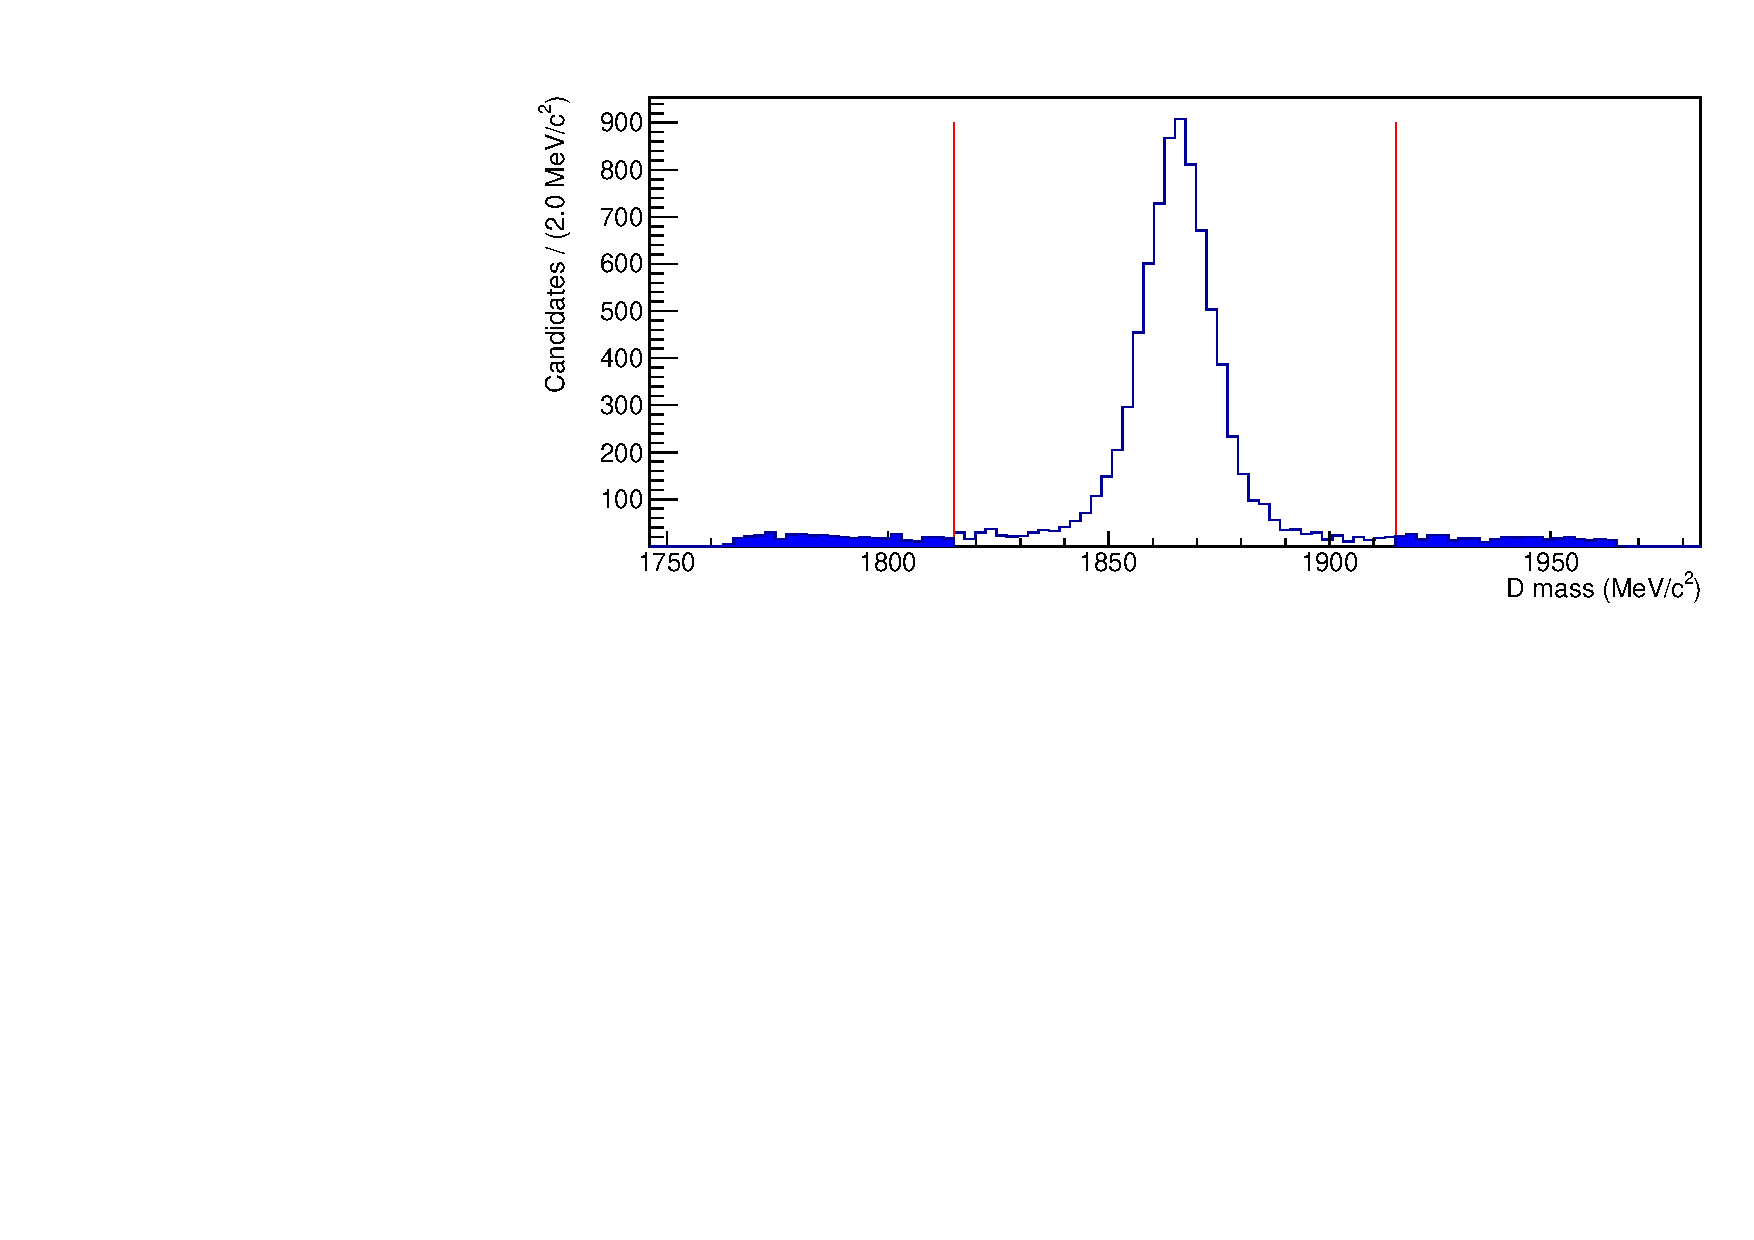
\includegraphics[width=0.8\linewidth]{figures/backgrounds/Dsidebands.pdf}
\caption{Reconstructed \Dz mass for \kpi DD candidates with \runone and \runtwo samples combined. The red lines indicate the values 50 \mevcc away from the nominal \Dz mass, and the bins shaded in blue represent the events that contribute to the \Dz mass sidebands. These events are expected to be dominated by charmless decays.}
\label{Dsidebands}
\end{figure}

A simple fit is performed to the invariant \B mass distribution, formed from the data in the \Dz mass sidebands, using a Gaussian to model the signal and an exponential shape to model the background. Variables that have been refitted with constraints are used in the selection, including the constraint that the \Dz is fixed to its known mass, which then favours events towards the true \Dz mass. This effectively removes the \Dz sidebands and therefore the charmless background cannot be estimated. In order to correctly estimate the background contribution in the \Dz mass sidebands, a modified selection is applied with the refitted vertex \chisq replaced with the vertex \chisq with no refit applied. For each \Dz decay mode, two fits are performed on data, one requiring the \Dz FD significance to be greater than zero and the other requiring it to be greater than 2, as shown in \fig\ref{charmlesspipi} for \pipi.

\begin{figure}
\centering
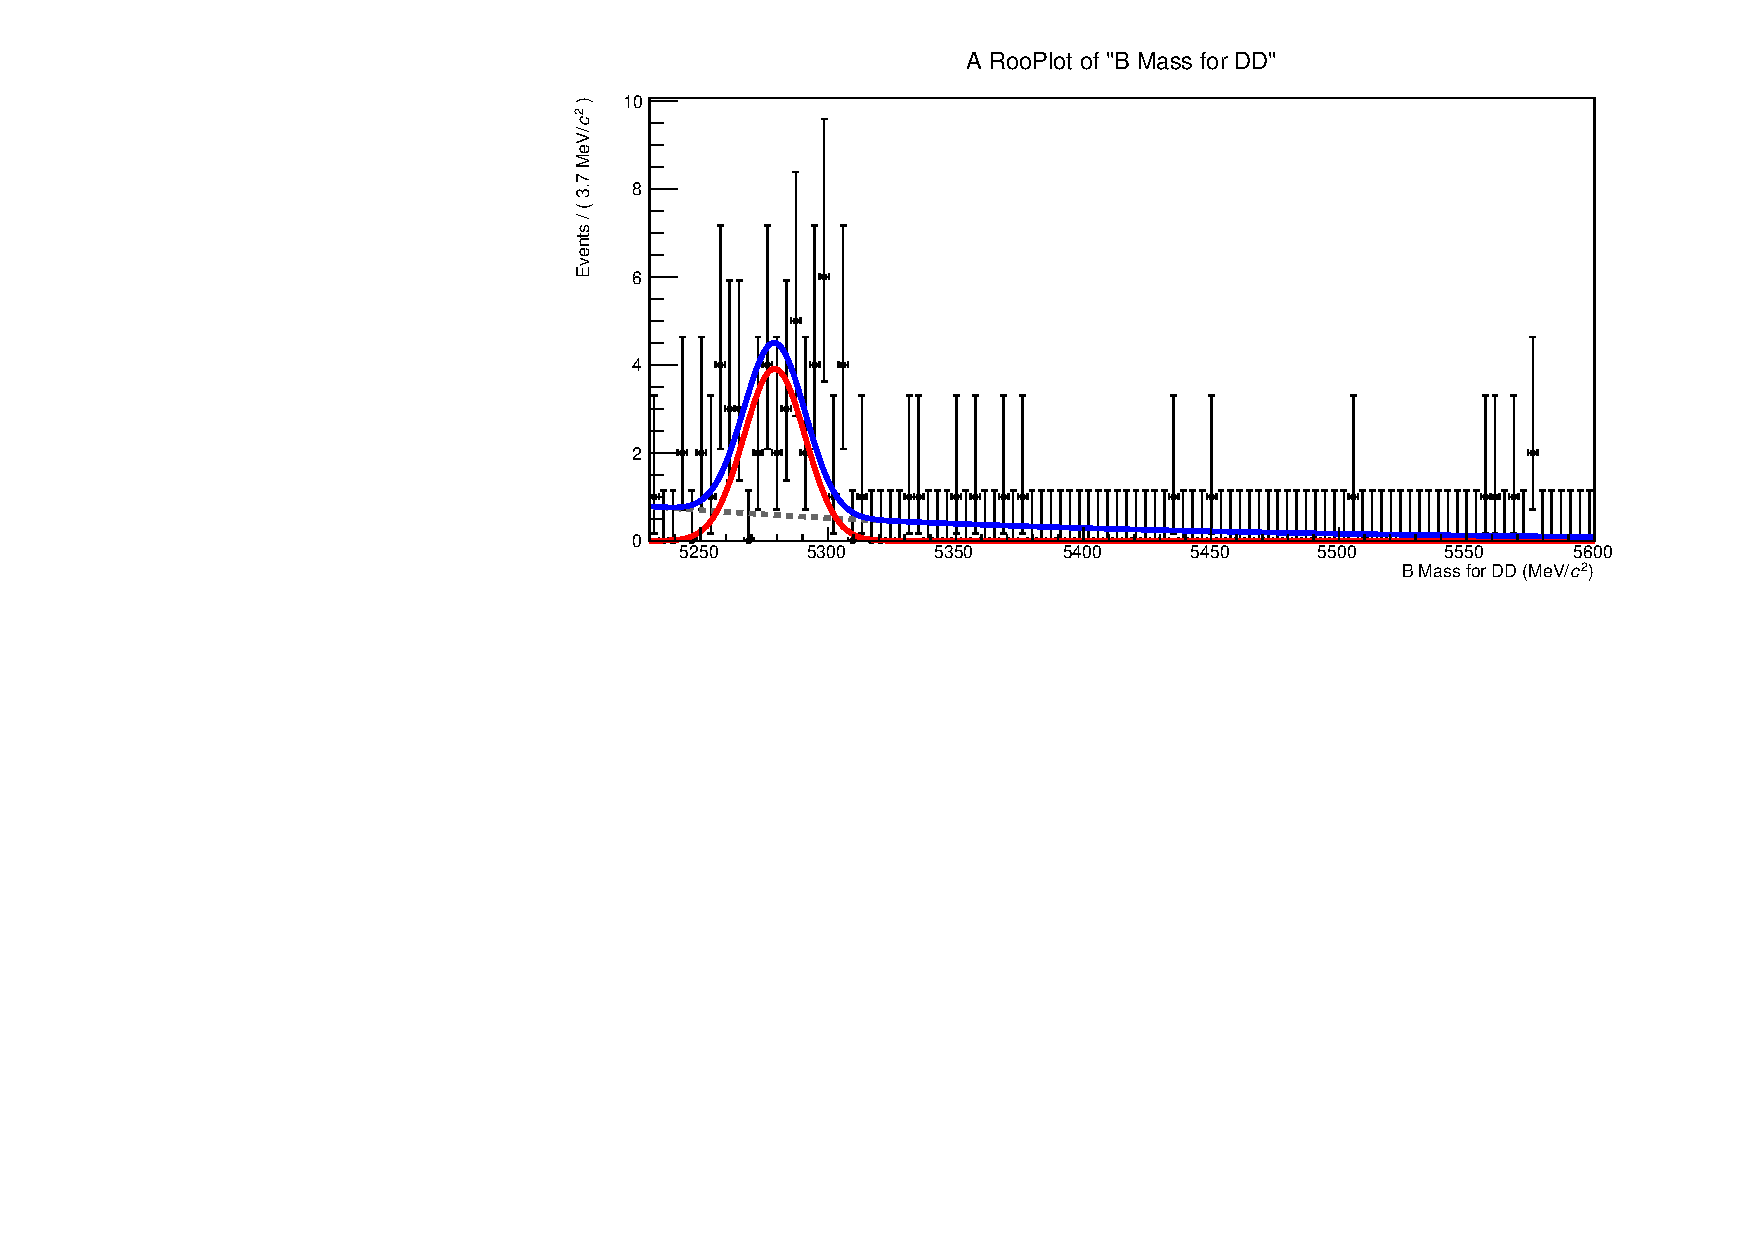
\includegraphics[width=0.7\linewidth]{figures/backgrounds/charmlessFit_PiPi_DD_FD0.pdf}
\put(-100,100) {(a)}
\hfill
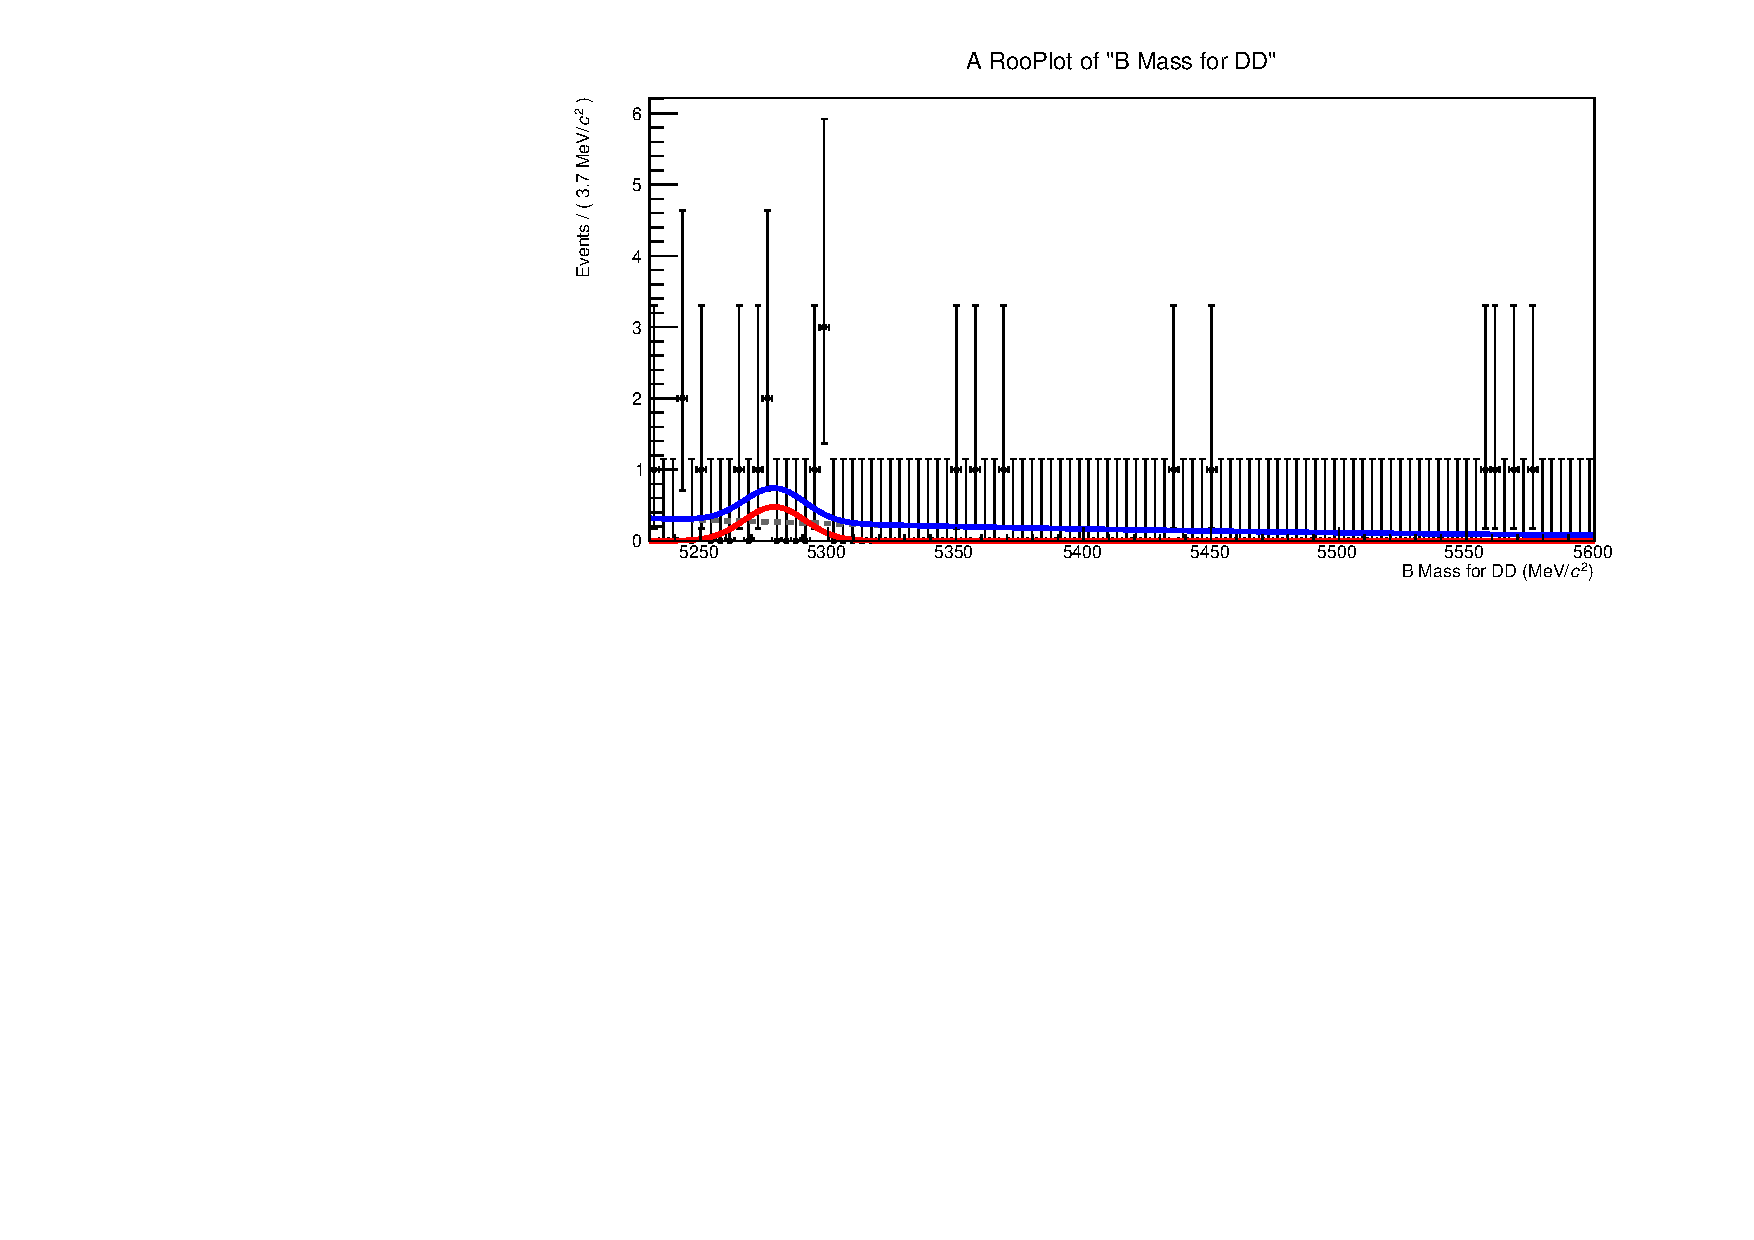
\includegraphics[width=0.7\linewidth]{figures/backgrounds/charmlessFit_PiPi_DD_FD2.pdf}
\put(-100,100) {(b)}
\caption{Fits, using the Run 1 data, to the refitted B mass taking \pipi candidates from the \Dz mass sidebands after requiring the FD significance to be (a) greater than 0 and (b) greater than 2. A Gaussian is used to model the signal and an exponential for the combinatorial background.}
\label{charmlesspipi}
\end{figure}

The fits in \fig\ref{charmlesspipi} give the yields of the \Bm mass peak in the \Dz mass sidebands, which are subsequently scaled to provide an estimate for this background within the \Dz mass window. By being able to quantify the number of charmless events expected in the \Bm mass spectrum after a given selection, it is possible to determine if the charmless background has been reduced to negligible levels. 

In the final selection, the \Dz FD significance is required to exceed 2, as all charmless contributions are consistent with zero under this requirement, which retains 72\% of the signal events. The expected yields of the charmless background in most of the two- and four-body \Dz decay modes are significantly less than 1\% of the signal yield and are therefore considered negligible. However, the estimated charmless contribution in the \pipi mode is greater than 1\% and so could affect the measurements. The \Dz FD significance requirement is not tightened further for the \pipi mode, as this would result in an extra 10\% loss in signal, which is deemed unacceptable. Instead the possible charmless contribution is considered as a source of systematic uncertainty; details are given in \sect\ref{sec:systematics}. 

\subsubsection{\boldmath \decay{\Bm}{\D\pim\pip\pim}}
\label{sec:backgrounds:b2dpipipi}

Now consider backgrounds that do not proceed via a \KS meson. In particular \decay{\Bm}{\D\pim\pip\pim} decays have a branching fraction of $5.7 \times 10^{-3}$~\cite{PDG2014} (about 50 times the signal \decay{\Bm}{\D\Kstarm(\KS(\pip\pim)\pim)} branching fraction), and are expected to occur as a peaking background underneath the signal. In order to remove this background, events are selected with the requirement that the \KS has travelled within the detector. For DD candidates this requirement is already satisfied, however for LL candidates a minimum requirement on the FD significance of the \KS meson, defined in \eqn\ref{FDdefinition}, is used to remove this background. 

The \decay{\Bm}{\D\pim\pip\pim} background is estimated by taking the \KS mass sidebands ($>$ 20 MeV from the nominal \KS mass) in data, with a modified selection applied that does not use any refitted variables, and performing a fit to the invariant \Bm mass distribution, as described for the charmless background. A Gaussian is used to model the signal and an exponential for the combinatorial background. This fit is performed on \kpi data, requiring the \KS FD significance to be greater than zero and 5, as shown in \fig\ref{strangelessfits}. Using these fits the estimated \decay{\Bm}{\D\pim\pip\pim} yield for \runtwo in the signal region with \KS FD significance $>$ 0 is $77 \pm 11$ events, however with \KS FD significance $>$ 5 the yield drops to $1.0 \pm 1.0$ events corresponding to 0.3\% of the signal yield. For the final selection, the \KS FD significance is required to be greater than 5, for LL candidates only, as it suppresses the \decay{\Bm}{\D\pim\pip\pim} background to a negligible level.

\begin{figure}
\centering
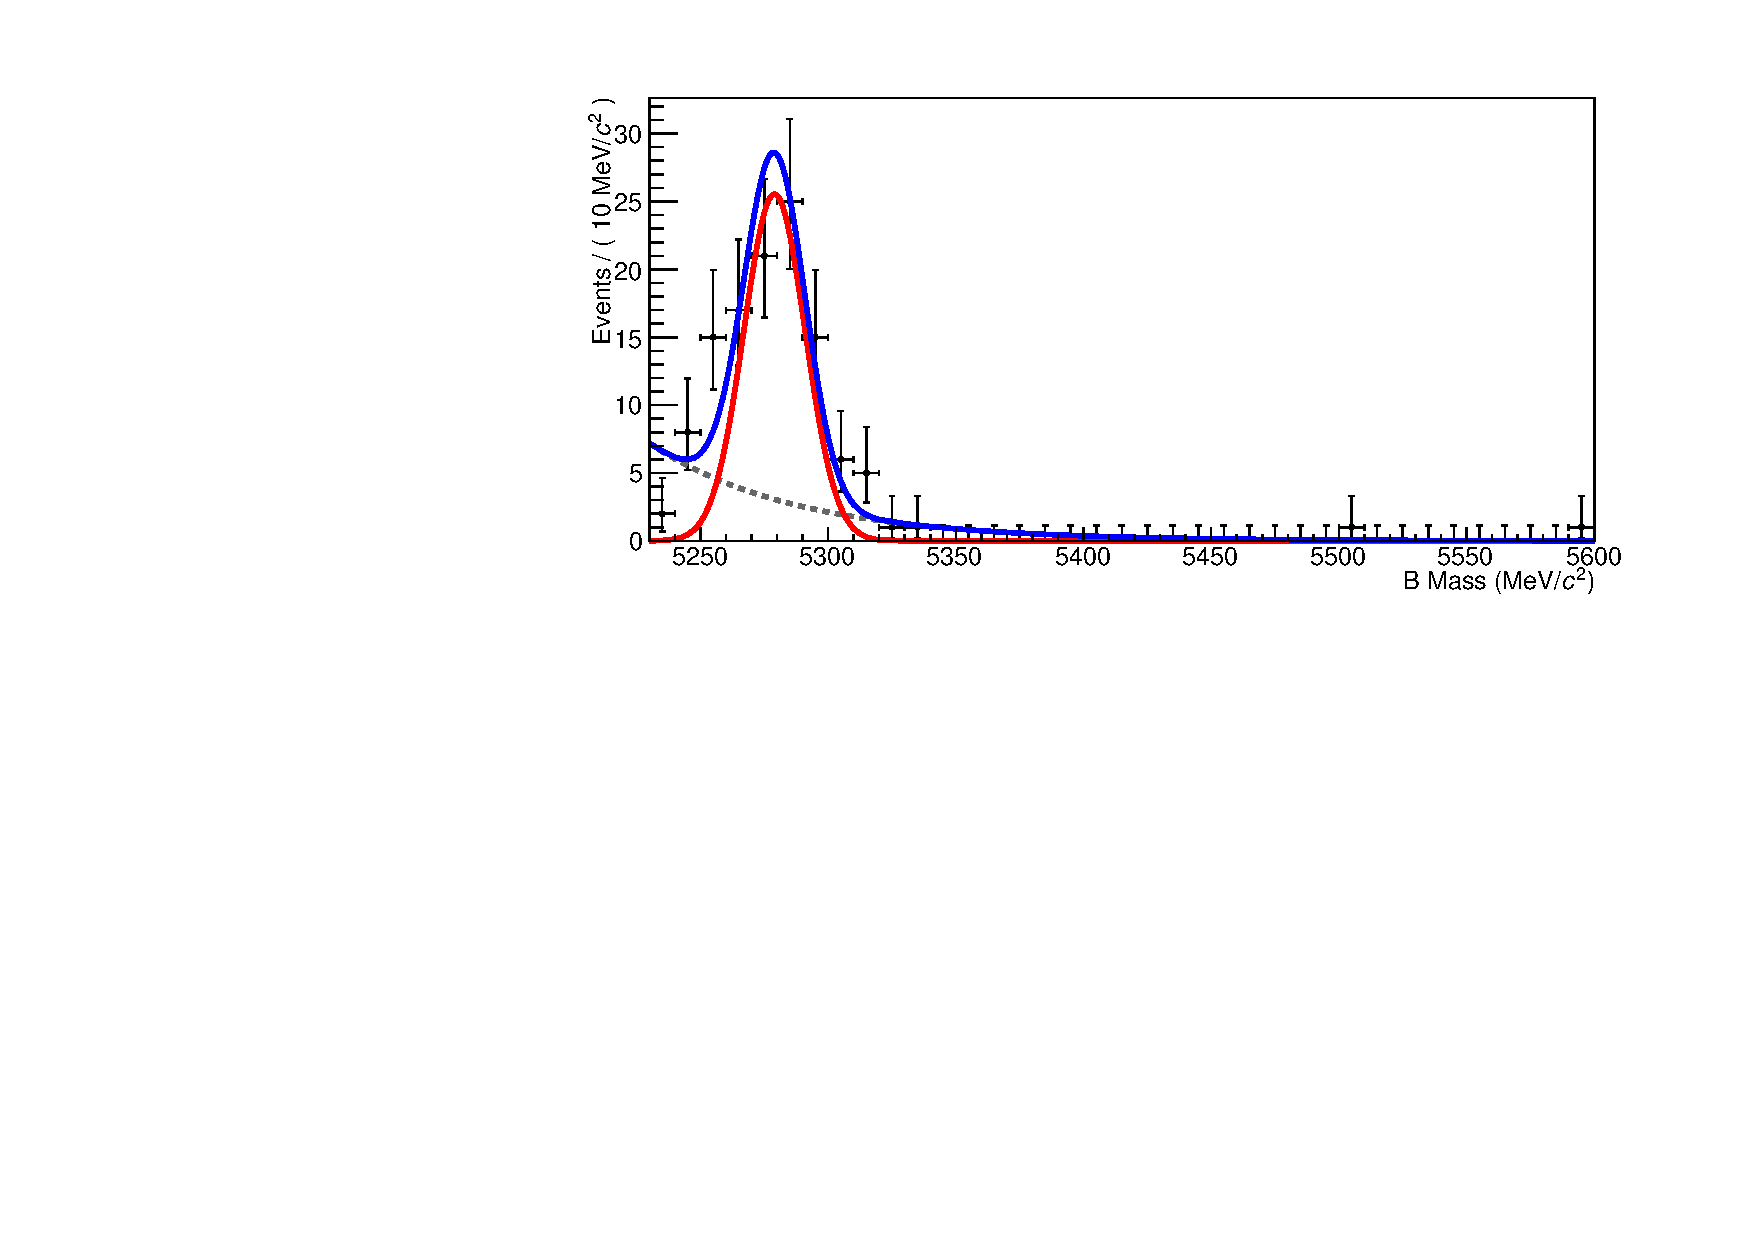
\includegraphics[width=0.7\linewidth]{figures/backgrounds/B2DpipipiFit_KPi_LL_FD0_run2.pdf}
\put(-100,100) {(a)}
\hfill
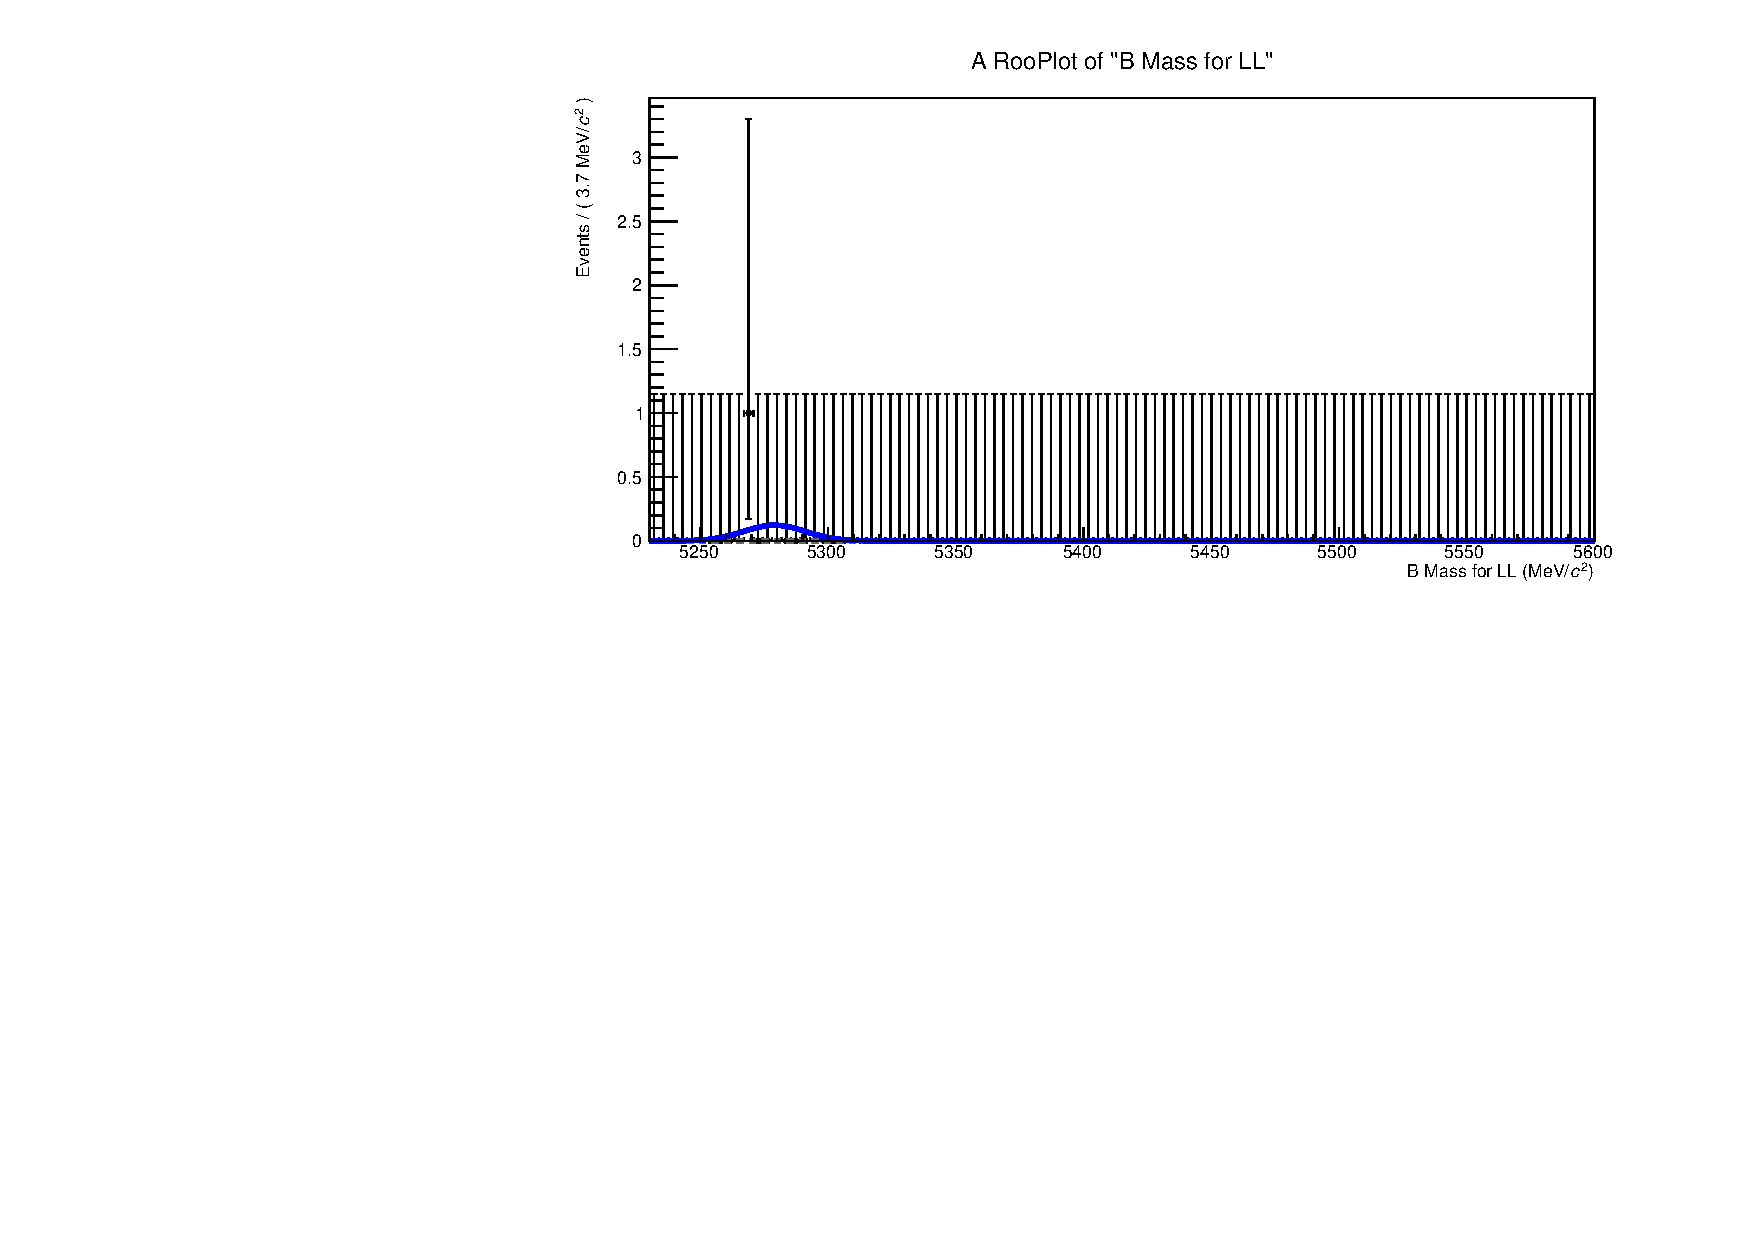
\includegraphics[width=0.7\linewidth]{figures/backgrounds/B2DpipipiFit_KPi_LL_FD5_run2.pdf}
\put(-100,100) {(b)}
\caption{Fits to the Run 2 refitted B mass taking \decay{\Dz}{\Km\pip} candidates from the \KS mass sidebands after requiring the FD significance to be (a) greater than 0 and (b) greater than 5$\sigma$.}
\label{strangelessfits}
\end{figure}

\subsubsection{Non-resonant \boldmath$B \to DK_s\pi$}
\label{sec:backgrounds:non-resonant}

The \Kstarm meson has a large natural width (about 50\mevcc~\cite{PDG2016}) therefore \decay{\Bm}{\D\KS\pim} decays may have a non-negligible contribution in this region, which could affect the measurement of \Pgamma. The purity of the \Kstarm in the sample can be increased firstly by only accepting \Kstarm candidates that have a reconstructed mass within 75~\mevcc of the known mass and secondly by exploiting the vector properties of the signal decay. 

As the \Kstarm meson is a vector meson, the \decay{\Bm}{\D\Kstarm} decay is a {\textit{Scalar $\to$ Vector Vector}} decay, forcing the \Kstarm to be longitudinally polarised due to the conservation of angular momentum. The structure of this decay can be observed using the \KS helicity angle, $\theta_{\KS}$, which is defined as the angle between the \KS and the \Bm meson momentum in the \Kstarm rest frame, as illustrated in \fig\ref{helicityangle}. This angle, $\cos(\theta_{\KS})$, follows a parabolic distribution for pure \decay{\Bm}{\D\Kstarm}, as shown in \fig\ref{helicitycut}.~\footnote{The \KS helicity angle distribution is not symmetric. The asymmetry in this variable, manifest in both data and simulation, is due to the momentum and transverse momentum selections placed on the bachelor pion at the stripping stage of the selection.}

\begin{figure}
\centering
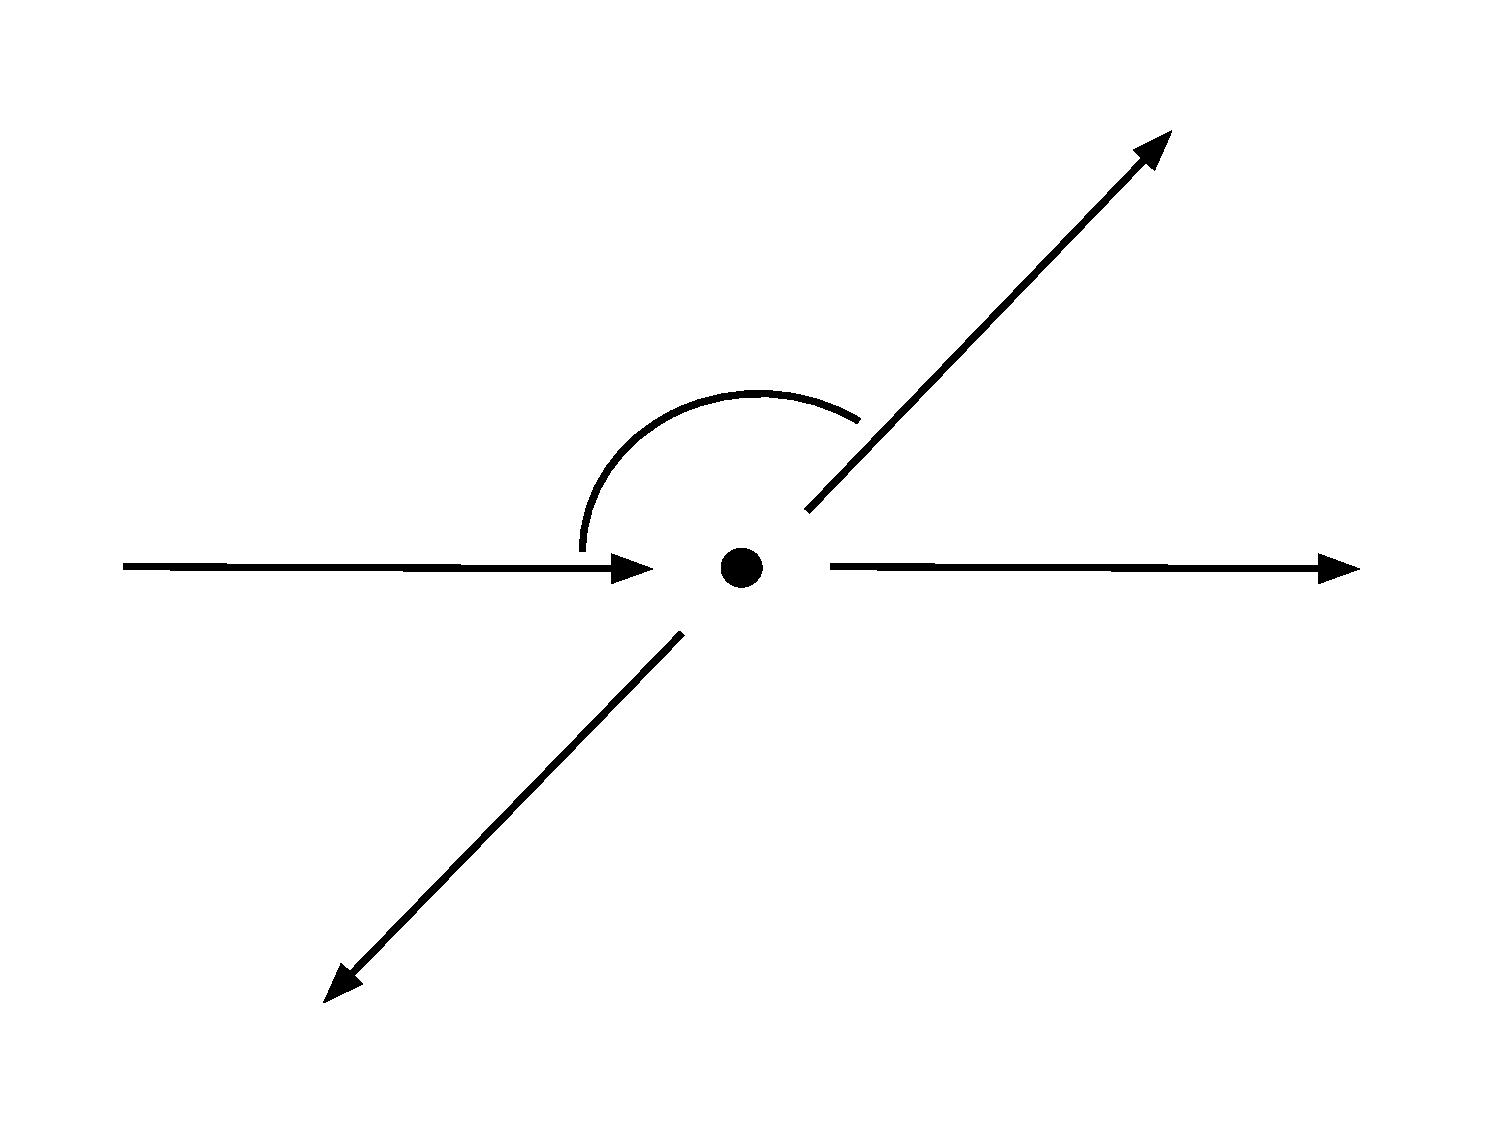
\includegraphics[width=0.5\linewidth]{figures/backgrounds/helicityangle.pdf}
\put(-200,85) {\Bm}
\put(-125,115) {$\theta_{\KS}$}
\put(-30,85) {\Dz}
\put(-75,140) {\KS}
\put(-165,40) {\pim}
\put(-100,60) {\Kstarm}
\caption{Diagram of \Bm decay particles in the \Kstarm rest frame, illustrating the definition of the \KS helicity angle, $\theta_{\KS}$.}
\label{helicityangle}
\end{figure}

\begin{figure}[h]
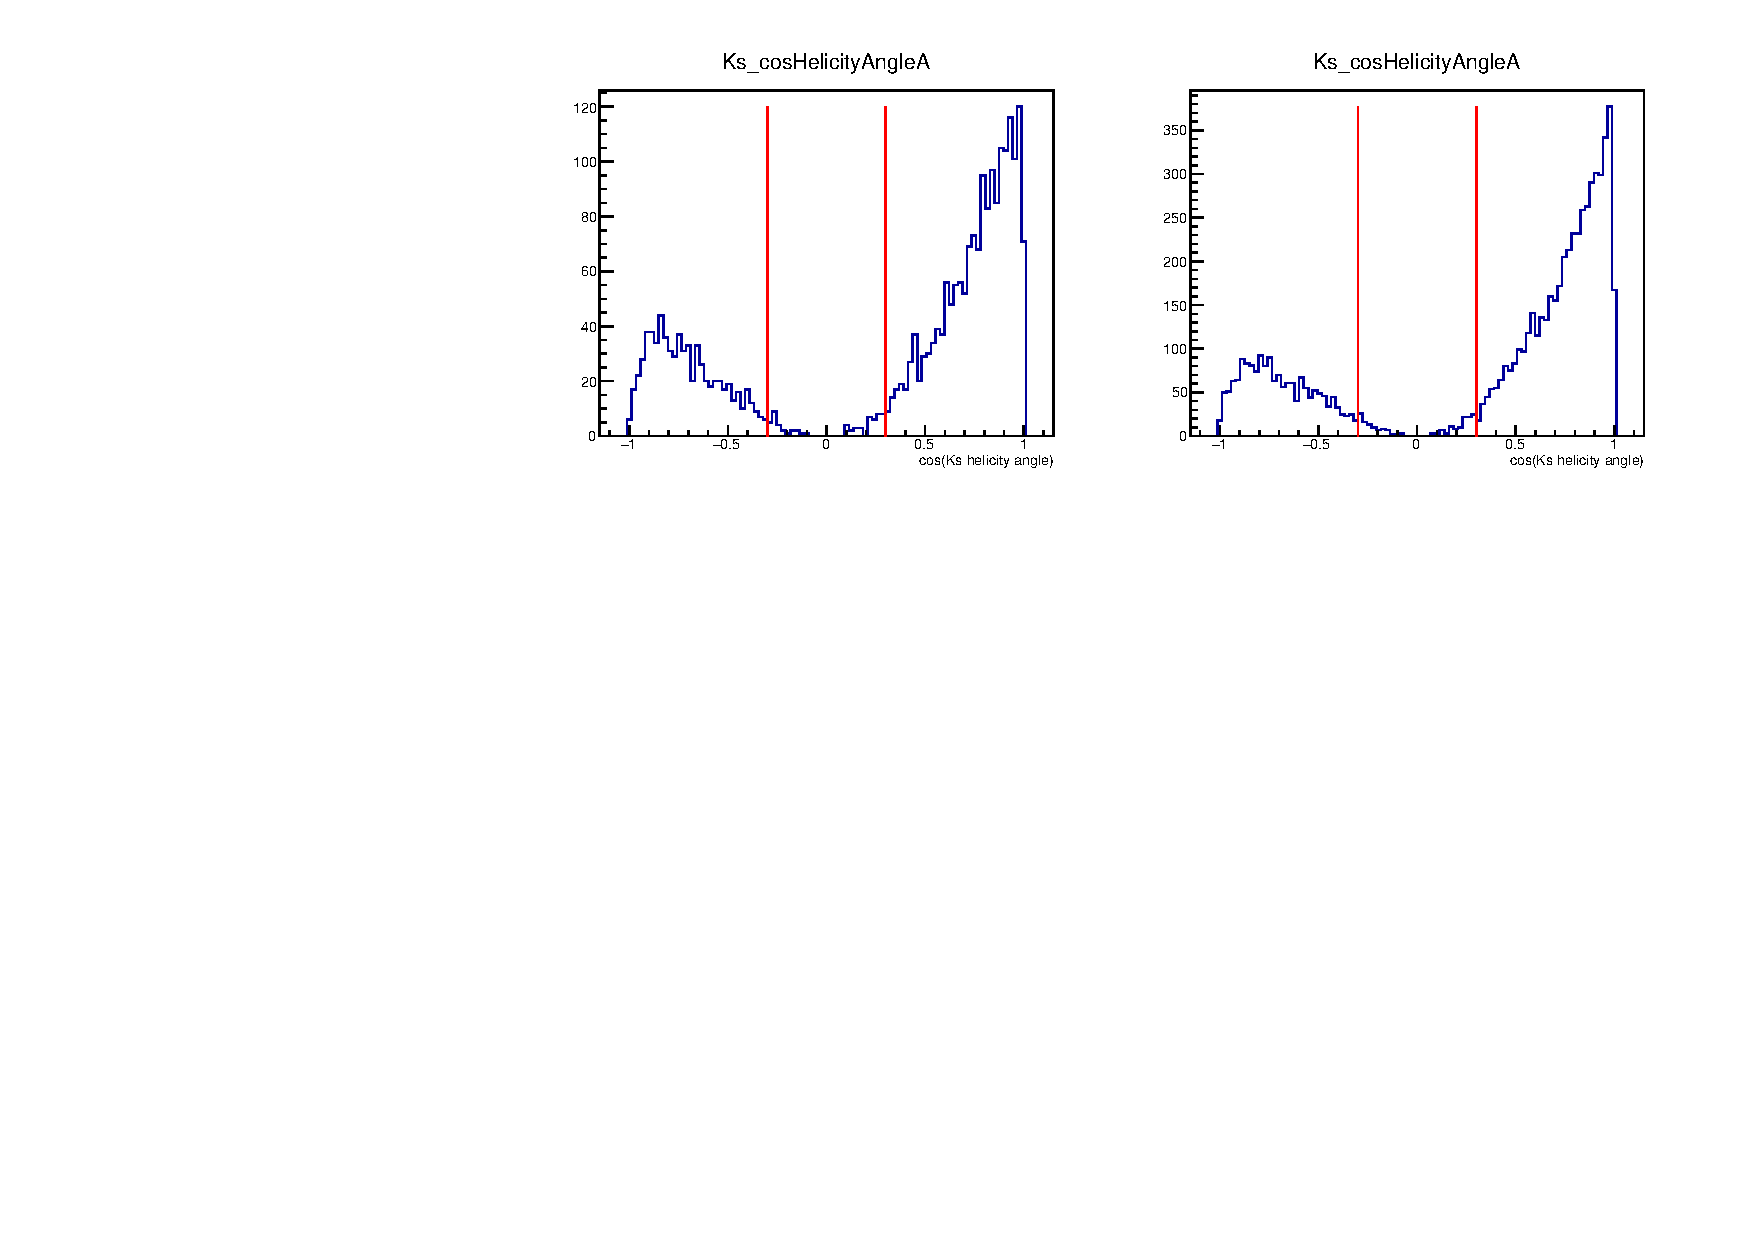
\includegraphics[width=\linewidth]{figures/backgrounds/KsHelicityCut.pdf}
\put(-380,100) {(a)}
\put(-170,100) {(b)}
\caption{Distribution of $\cos(\theta_{\KS})$ from a simulated sample of \kpi events for (a) LL candidates and (b) DD candidates. The red lines represent the region $\cos(\theta_{\KS})$ that is rejected in the selection.}
\label{helicitycut}
\end{figure}

By removing candidates that have a small absolute value of $\cos(\theta_{\KS})$, a large amount of non-resonant \decay{\Bm}{\D\KS\pim} and combinatorial background can be removed while retaining almost all of the pure \decay{\Bm}{\D\Kstarm} signal. The combinatorial background is roughly uniform in $\cos(\theta_{\KS})$, as shown in \fig\ref{Kshelicitybkg}. Removing events with an absolute value of $\cos(\theta_{\KS})$ less than 0.3 retains 97\% of true \decay{\Bm}{\D\Kstarm} decays, while rejecting 30\% of the combinatorial background. This $\cos(\theta_{\KS})$ selection would also be expected to remove 33\% of the non-resonant \decay{\Bm}{\D\KS\pim} background. The optimisation of the \Kstarm mass and \KS helicity angle selection is discussed in \sect\ref{sec:cpfit:optimisation}.

\begin{figure}
\centering
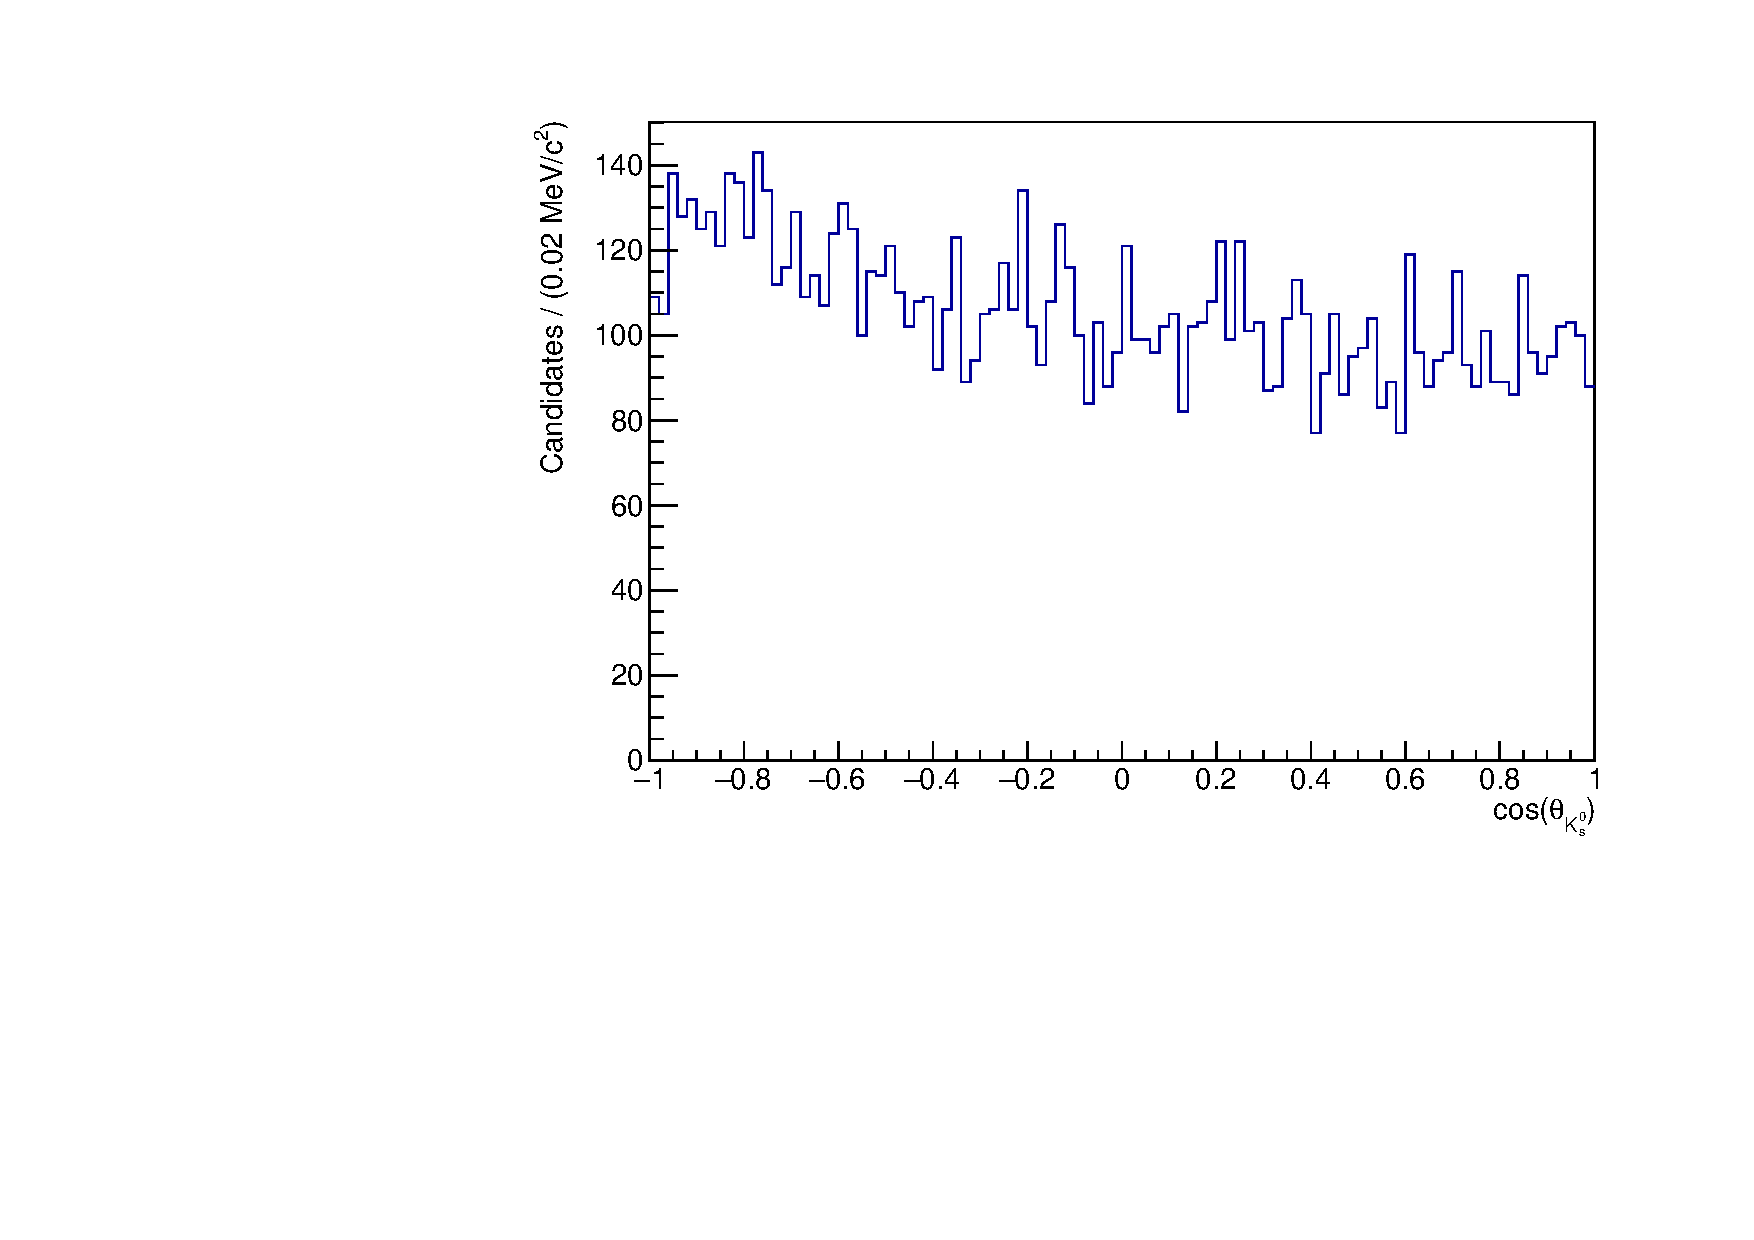
\includegraphics[width=0.5\linewidth]{figures/backgrounds/Kshelicity_background.pdf}
\caption{Distribution in data of the cosine of \KS helicity angle in \kpi combinatorial background.}
\label{Kshelicitybkg}
\end{figure}

\subsubsection{Crossfeed background}
\label{sec:backgrounds:crossfeed}

As discussed in \sect\ref{sec:selection:pid}, the \Bm mass spectrum for the doubly Cabibbo suppressed ADS mode, \pik, can contain background events from the favoured \kpi mode, where the \Dz daughter mass hypotheses are swapped, i.e. the kaon is misidentified as a pion and the pion is misidentified as a kaon. When considering the two-body \Dz decay modes, the favoured \kpi mode has a branching ratio 281 times higher than the \pik mode~\cite{PDG2016}. Particle identification requirements on the \Dz daughters, detailed in \sect\ref{sec:selection:pid}, significantly reduce this background, however in order to bring it down to negligible levels a veto must be applied. An alternative \Dz mass, $m(D_{\text{swapped}})$, is calculated where the \Dz meson is reconstructed with both daughter mass hypotheses are swapped. The applied veto requires $m(D_{\text{swapped}})$ to be greater than 15~\mevcc away from the known \Dz mass. This veto is illustrated in \fig\ref{Dmassveto}, which shows the distributions from simulated samples for DD candidates in Run 1. \Fig\ref{Dmassveto} (a) is the \Dz mass distribution with the correct daughter mass hypothesis, therefore this is what the $m(D_{\text{swapped}})$ distribution would look like for the doubly misidentified background. Similarly, \fig\ref{Dmassveto} (b) is the \Dz mass distribution with the swapped daughter mass hypothesis, therefore this is what the $m(D_{\text{swapped}})$ distribution would look like for the signal. The veto removes 91.2\% of doubly misidentified background, corresponding to events that lie within the red lines in \fig\ref{Dmassveto} (a), while maintaining a 92.5\% signal efficiency, corresponding to events that lie outside the red lines in \fig\ref{Dmassveto} (b). The two-body veto is only applied to the \pik mode in this analysis.
 
\begin{figure}[h]
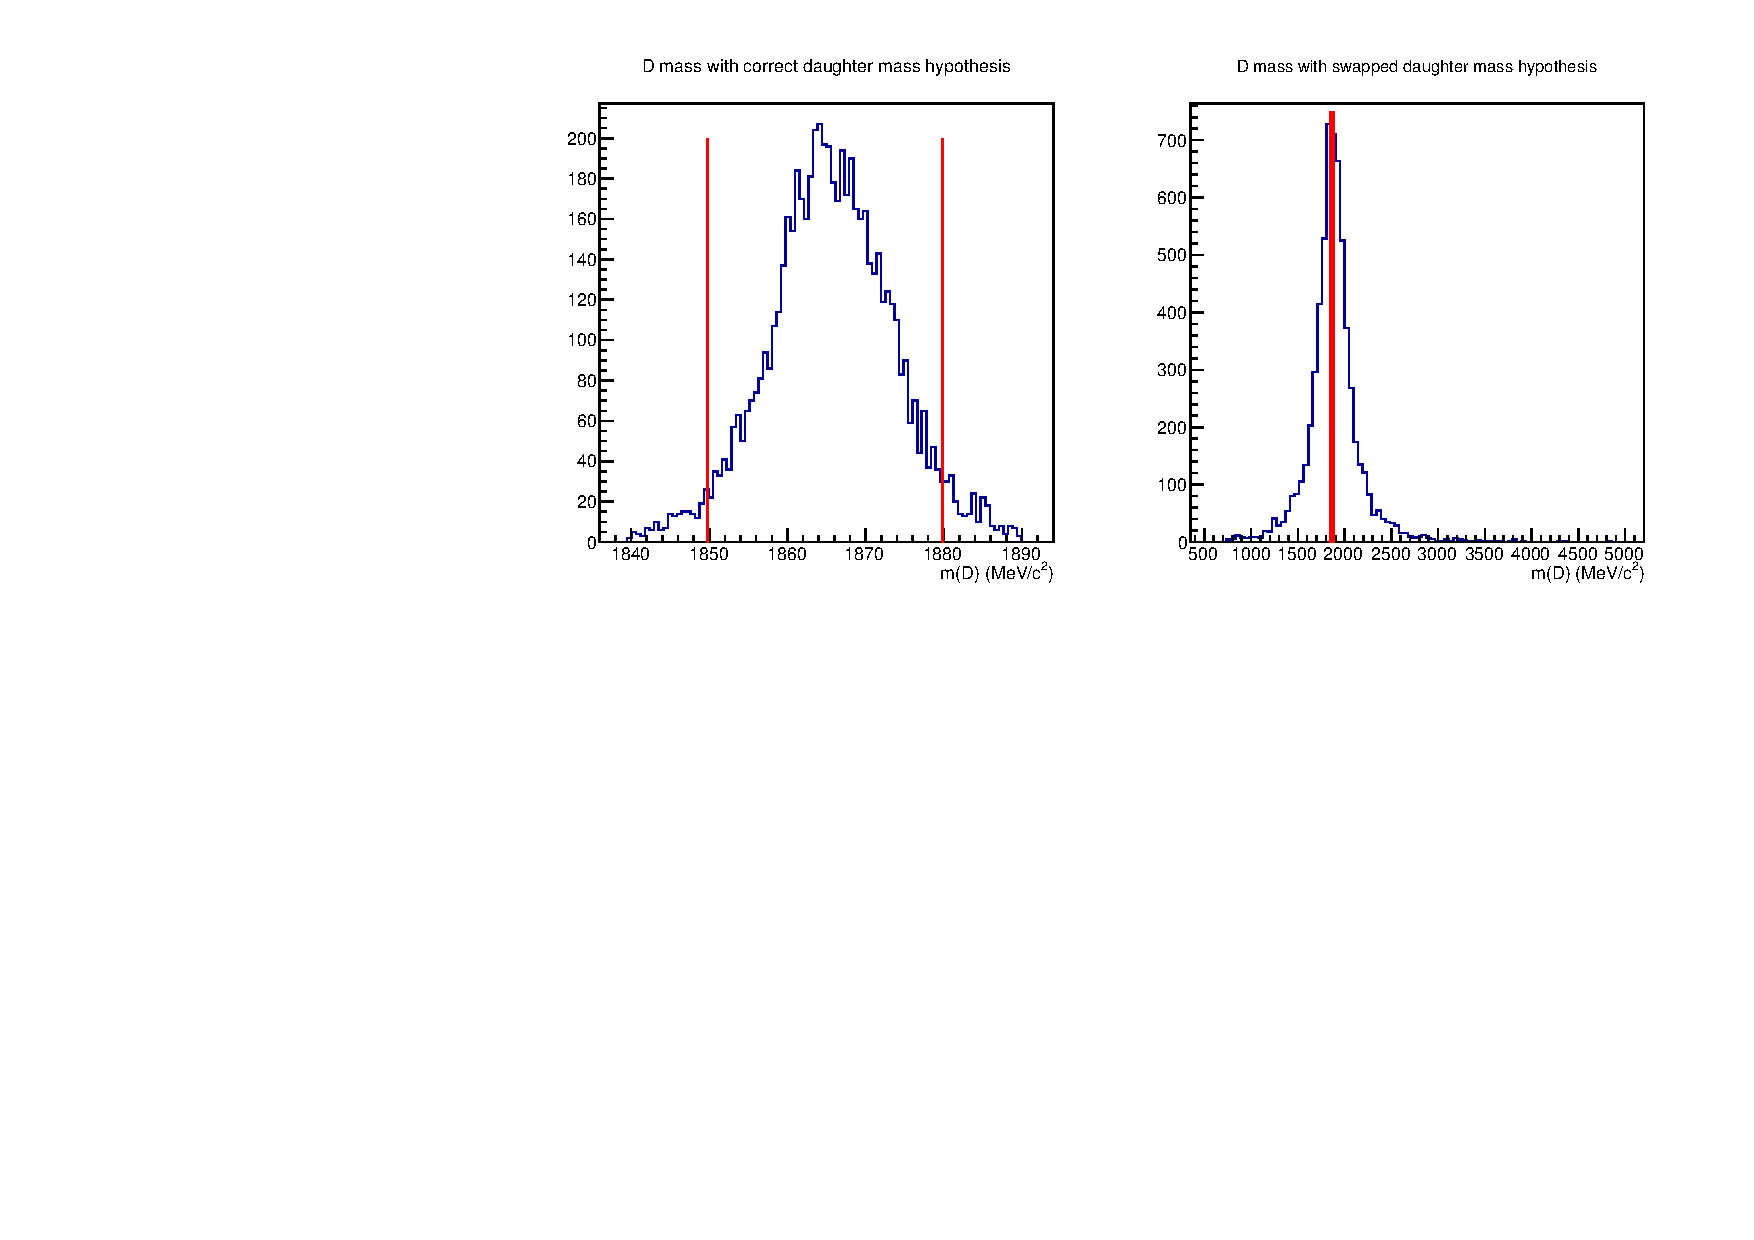
\includegraphics[width=\linewidth]{figures/backgrounds/Dmassveto.pdf}
\put(-380,150) {(a)}
\put(-170,150) {(b)}
\caption{Distributions from simulated samples of DD candidates in Run 1 showing \Dz mass with (a) the correct \Dz daughter mass hypothesis and (b) the swapped \Dz daughter mass hypothesis. Events within the red lines correspond to those removed by the double misidentification veto applied to the \pik mode.}
\label{Dmassveto}
\end{figure}

For the four-body modes, the equivalent background can appear in the suppressed \pikpipi mode due to contamination from the favoured \kpipipi. In this case, there are two \pip mesons that could be misidentified as a \Kp meson, therefore two vetos are applied. The two possible alternative \Dz masses are reconstructed as a swapped mass hypothesis, one where the kaon is swapped with the lower momentum pion, $m(D_{\text{swapped}}^{\text{low p}})$, and the other where the kaon is swapped with the higher momentum pion, $m(D_{\text{swapped}}^{\text{high p}})$. The veto is applied to both these reconstructed masses as demonstrated in \fig\ref{Dmassveto4body}. The four-body veto is only applied to the \pikpipi mode in this analysis.

\begin{figure}[h]
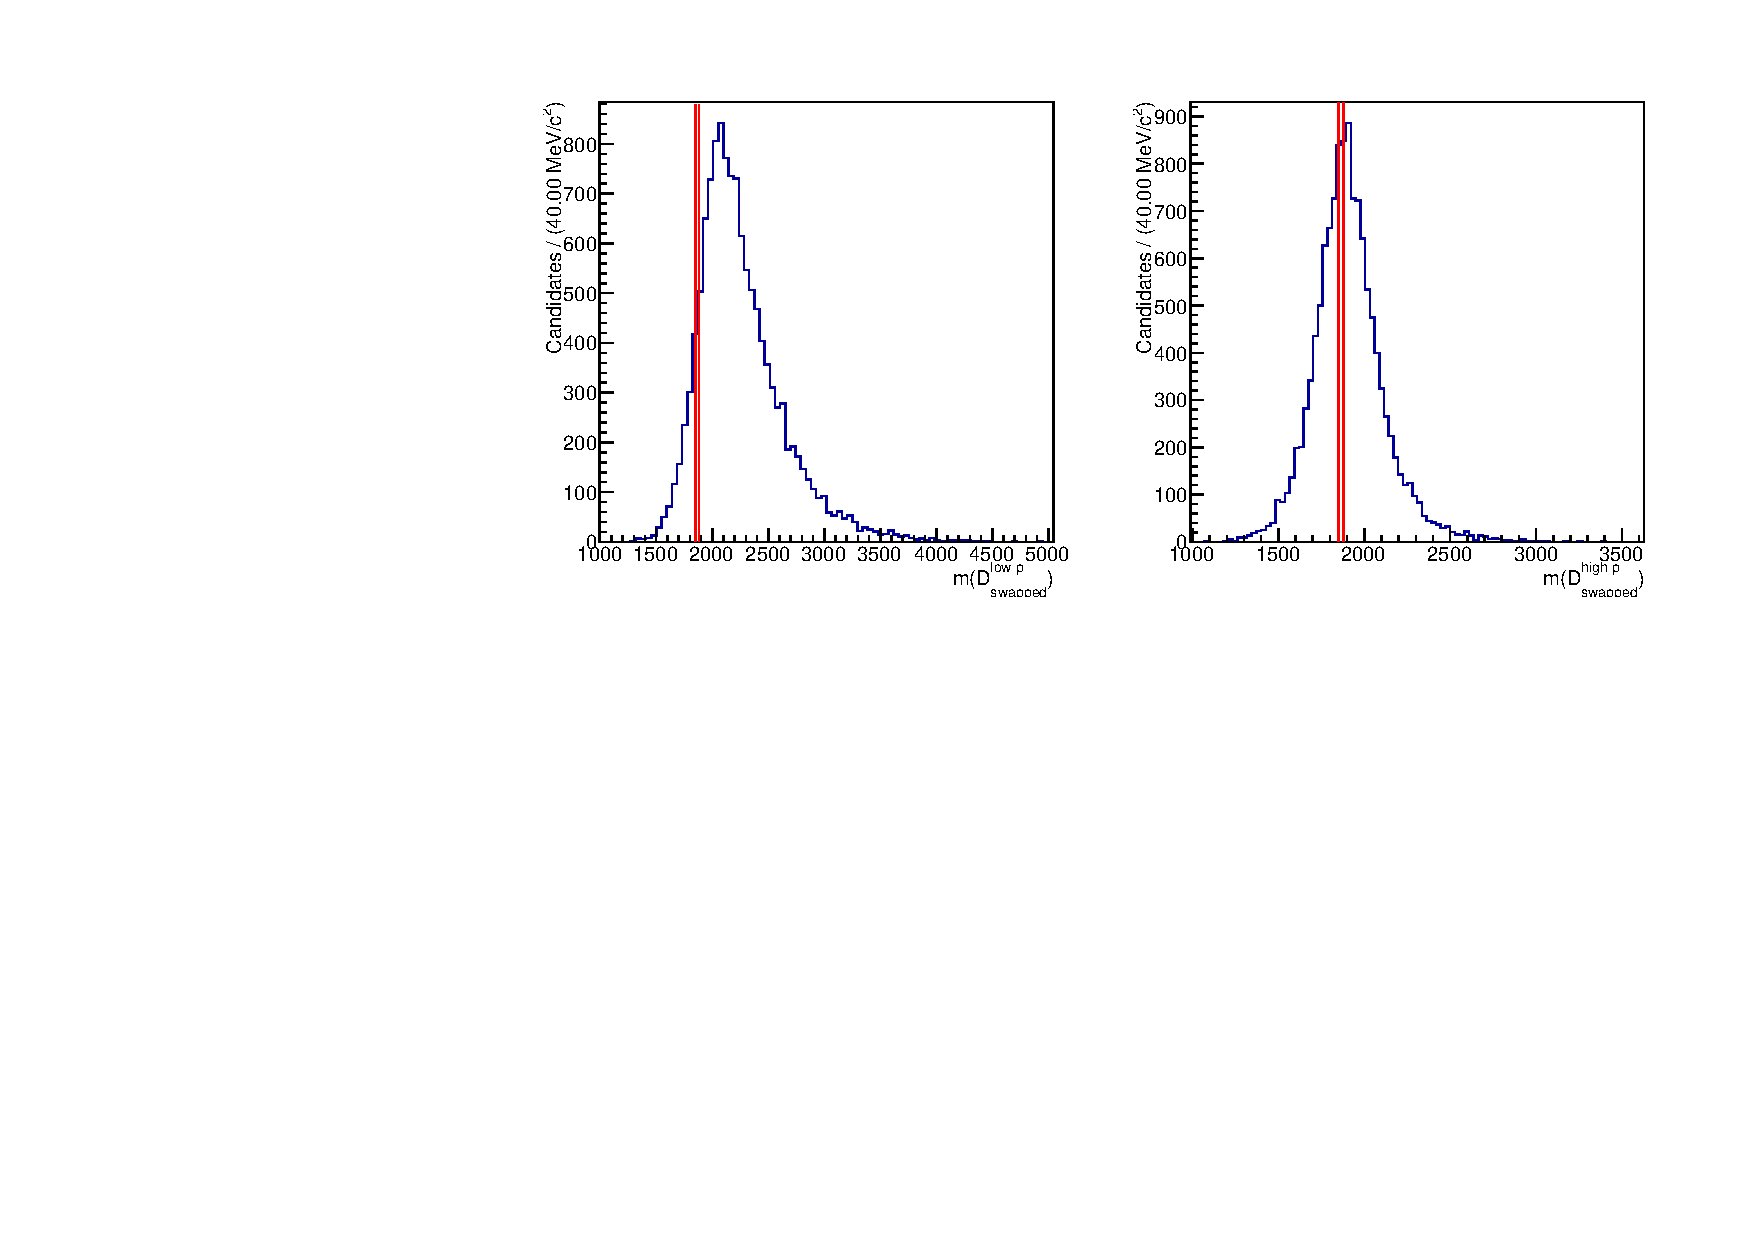
\includegraphics[width=\linewidth]{figures/backgrounds/Dmassveto_4body.pdf}
\put(-380,150) {(a)}
\put(-170,150) {(b)}
\caption{Distributions from simulated samples of DD candidates in Run 2 showing the swapped \Dz daughter mass hypothesis where (a) the kaon is swapped with the lower momentum pion and (b) the kaon is swapped with the higher momentum pion. Events within the red lines correspond to those removed by the double misidentification veto to the suppressed \pikpipi mode.}
\label{Dmassveto4body}
\end{figure}

In addition to the double misidentification veto, the selection requirement on the reconstructed \Dz mass and the PID requirements, discussed in Secs.~\ref{sec:selection:strippingandtrigger} and \ref{sec:selection:pid}, both help to reduce the crossfeed background. In order to determine the overall crossfeed contamination in the suppressed \pik mode, the efficiency of the \Dz mass window, double misidentification veto and PID requirements are taken into account for both the normal and swapped \Dz mass hypotheses. Tables~\ref{crossfeedtwobody} and \ref{crossfeedfourbody} show the expected proportion of crossfeed events in both the two- and four-body ADS modes, relative to the signal. These results show that the crossfeed background is negligible at less than 0.1\% of the signal.

\begin{table}
\centering
\begin{tabular}{c|cc}
& \runone & \runtwo \\
\hline
LL & $9.5 \times 10^{-3}$ & $5.6 \times 10^{-3}$ \\
DD & $6.5 \times 10^{-3}$ & $5.3 \times 10^{-3}$ \\
\end{tabular}
\caption{The proportion \kpi events expected in the \Bm mass spectrum of the suppressed \pik mode relative to the total \pik signal yield.}
\label{crossfeedtwobody}
\end{table}

\begin{table}
\centering
\begin{tabular}{c|cc}
& \runone & \runtwo \\
\hline
LL & $2.7 \times 10^{-3}$ & $1.4 \times 10^{-3}$ \\
DD & $1.0 \times 10^{-3}$ & $6.3 \times 10^{-4}$ \\
\end{tabular}
\caption{The proportion \kpipipi events expected in the \Bm mass spectrum of the suppressed \pikpipi mode relative to the total \pikpipi signal yield.}
\label{crossfeedfourbody}
\end{table}


\subsubsection{\boldmath \decay{\Lb}{\Lc\Kstar} background in the \kk mass spectrum}
\label{sec:backgrounds:Lb2LcKst}

An additional source of background in the \kk mass spectrum comes from the decay \decay{\Lb}{\Lc(p\Km\pip)\Kstarm}, where the proton is misidentified as \Kp and the \pip is missed in the reconstruction. The decay mode \decay{\Lc}{p\Km\pip} accounts for over 6\% of the \Lc branching fraction~\cite{PDG2016}, whereas \Lc decays that may contribute as background to the other \Dz decay modes, e.g. \decay{\Lc}{p\pim\pip}, are suppressed by an order of magnitude. Therefore, the \Lb background is only considered for the \kk decay model.

%The branching fraction of \decay{\Lb}{\Lc(p\kaon\pi)\Kstarm} is roughly five times larger than the \kk branching fraction. 
As the \decay{\Lb}{\Lc(p\kaon\pi)\Kstarm} and \kk decays have similar topologies, the selection efficiencies are expected to be similar, with the exception of the requirement on the reconstructed \Dz mass, which significantly reduces this background. Additionally, the background is slightly reduced by the PID requirements on the \Dz daughters, as the proton has to be incorrectly identified as a \Kp meson. Taking these considerations into account, the \Lb background is expected to contribute O(1) event to the \kk mass spectrum, discussed in \sect\ref{sec:cpfit:Lb2LcKst}. The PID requirements on the \Dz daughters cannot be increased to ensure this background is reduced to negligible levels, due to the effect on the signal efficiency. Therefore, in order to account for the \Lb background, it is modelled and included as a component to the fit, discussed in \sect\ref{sec:cpfit:Lb2LcKst}. 

\subsubsection{\boldmath \decay{\Bs}{\Dzb\bar{K}^{*}(1410)^0} background}
\label{sec:backgrounds:bs}

The decay \decay{\Bs}{\Dzb\bar{K}^{*}(1410)^0}, \decay{\bar{K}^{*}(1410)^0}{K^{*}(892)^-\pip}, where the \pip is missed in reconstruction is a possible background contribution. The branching fraction of this mode is similar to that of the signal and the same particles are present, therefore this background could be significant. Due to this background having the favoured mode corresponding to the combination of \Dzb and \Kstarm, it is considered as a contribution in the ADS mode. As the reconstruction of this background in the ADS mode requires the \pip meson to be missed, the reconstructed \Bm mass would fall in a region just below the signal peak. The fit used to extract the \CP observables has a lower mass limit of 5230\mevcc, therefore this background will be almost entirely removed. However, it is possible that a small contribution still remains in the signal region. 

The \decay{\Bs}{\Dzb\bar{K}^{*}(1410)^0} background contribution can be estimated from its branching fraction, $\left(3.9 \pm 3.5\right) \times 10^{-4}$~\cite{PDG2016}, and its efficiency through the \btodkst selection. Due to the similar topologies of the signal and background decays, the selection efficiency of the \decay{\Bs}{\Dzb\bar{K}^{*}(1410)^0} is taken to be the same as for \btodkst, except for the efficiency of the requirement that the \Bm mass must be above 5230\mevcc, given by $\epsilon_{\Bs}(B\ mass\ > 5230\mevcc)$. This assumption allows an estimate for the upper limit of the background contribution as a fraction of the signal yield, given by 

\begin{multline}
\frac{N(\decay{\Bs}{\Dzb\bar{K}^{*}(1410)^0})}{N(\btodkst)} = \frac{\BF(\decay{\Bs}{\Dzb\bar{K}^{*}(1410)^0})}{\BF(\btodkst)} \\ \times \frac{\epsilon_{\Bs}(B\ mass\ > 5230\mevcc)}{\epsilon_{\Bm}(B\ mass\ > 5230\mevcc)} \text { .}
\label{Bscalc}
\end{multline}
In order to calculate the efficiency, $\epsilon_{\Bs}(B\ mass\ > 5230\mevcc)$, a simulated sample of \decay{\Bs}{\Dzb\bar{K}^{*}(1410)^0}, \decay{\bar{K}^{*}(1410)^0}{K^{*}(892)^-\pip} events is generated, where the \pip is missed in reconstruction. The efficiency for the \Bm mass being greater than 5230\mevcc is found to be $6.4 \times 10^{-4}$. 

%The resulting calculation gives an upper limit estimate of $2.6 \pm 2.6$ \decay{\Bs}{\Dzb\bar{K}^{*}(1410)^0} events in \pik mode above 5230\mev. 
The calculation using \eqn\ref{Bscalc} gives an upper limit estimate of the background yield as a fraction of the ADS signal yield of $(1.28 \pm 1.26) \times 10^{-3}$ above 5230\mev. This estimated \Bs background is used to assign a systematic uncertainty to the \CP observables, discussed in \sect\ref{sec:systematics}.


\subsubsection{Lambda contamination}
\label{sec:backgrounds:contamination}

The \decay{\KS}{\pip\pim} decay could have contamination coming from \decay{\Lz}{\proton\pim}, where the proton is reconstructed as a pion. In order to distinguish between \KS decays and \Lz contamination, the Armenteros-Podolanski (AP) plot is used~\cite{APplot}. The transverse momentum of the daughters with respect to the mother particle, $p_T$, is plotted as a function of the longitudinal momentum asymmetry, defined as

\begin{equation}
\frac{p_L^+ - p_L^-}{p_L^+ + p_L^-} \text{ ,}
\label{longitudinalpasy}
\end{equation}
where $p_L^{\pm}$ is the longitudinal momentum of the positive (negative) daughter particles with respect to the direction of the mother. The decay products of the \decay{\KS}{\pip\pim} decay have the same mass and therefore on average their momenta is symmetrically distributed. For the \decay{\Lz}{\proton\pim}, the proton would, on average, take a larger proportion of the momentum resulting in an asymmetric distribution. Contamination from \Lz baryons would be clearly seen as a distinct structure on the AP plot, as illustrated in \fig\ref{apexample}. 

\begin{figure}
\centering
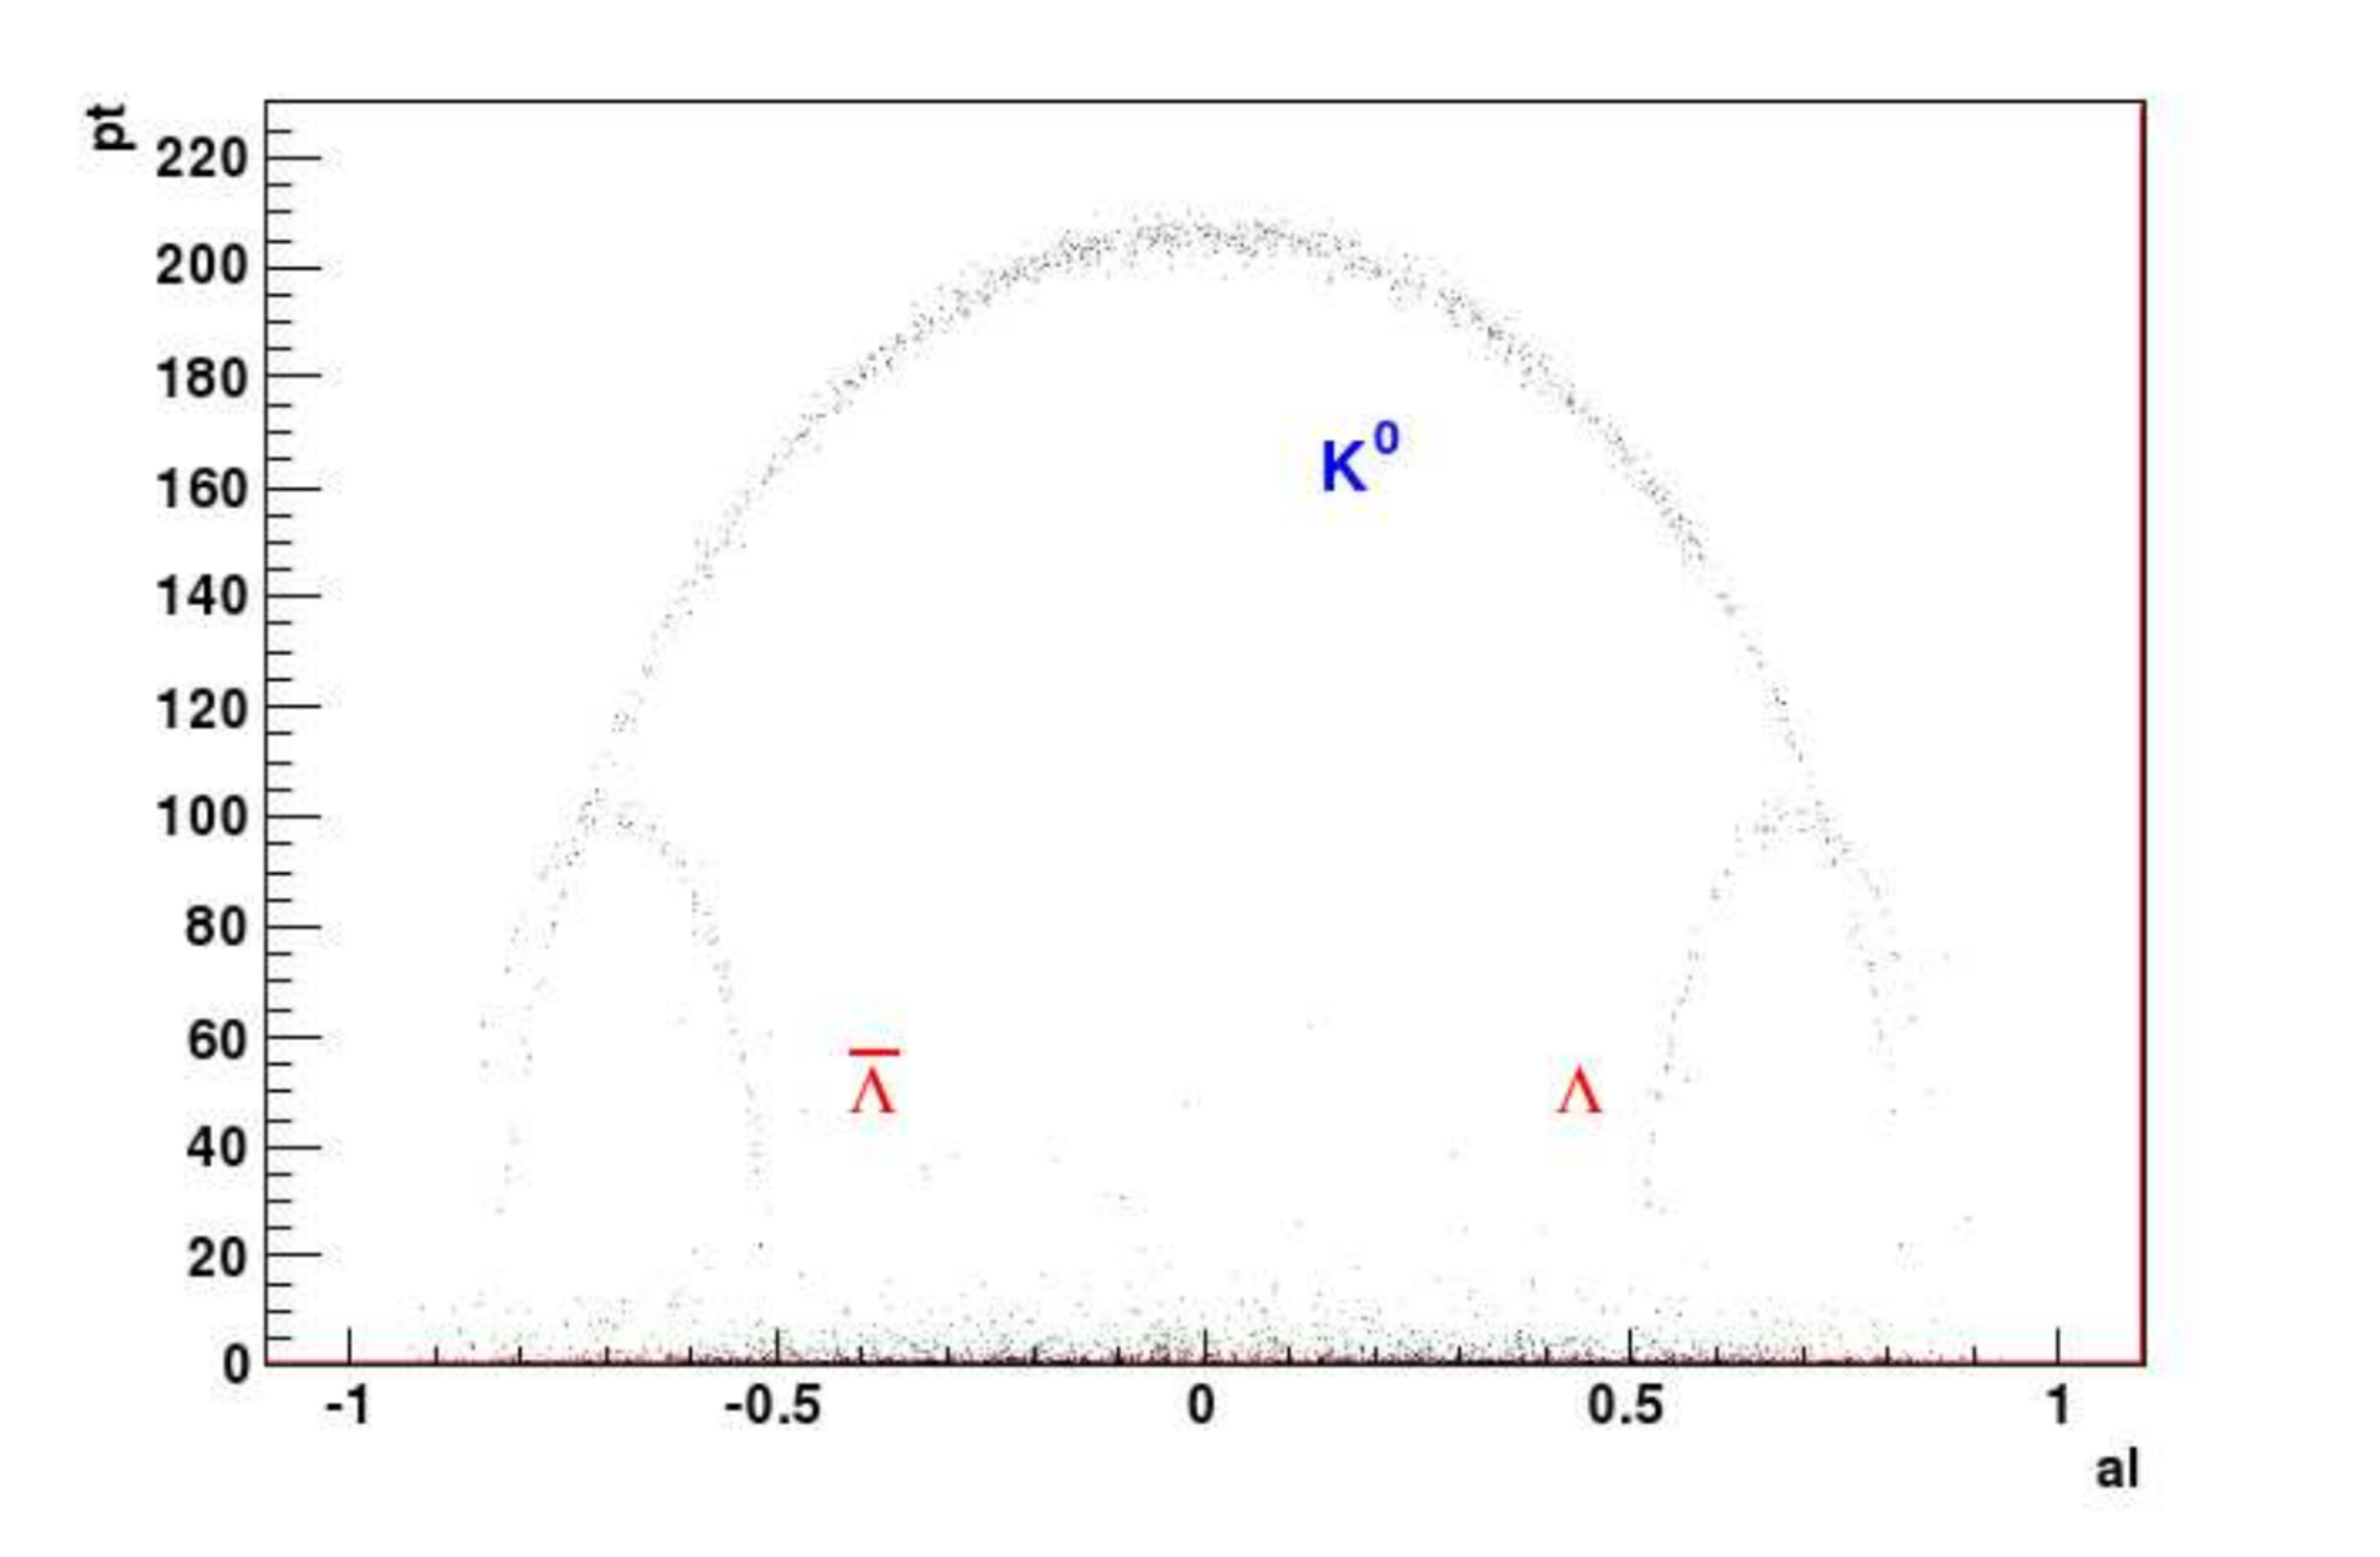
\includegraphics[width=0.5\linewidth]{figures/backgrounds/APfromPaper.pdf}
\caption{An example Armenteros-Podolanski plot showing where the signal regions for \KS, \Lz and \Lbar are located in the AP plane. Reproduced from Ref.~\cite{APplot}. The $pt$ label on the $y$ axis refers to the transverse momentum of the daughters with respect to the mother particle and the $al$ on the $x$ axis refers to the longitudinal momentum asymmetry, defined in \eqn\ref{longitudinalpasy}.}
\label{apexample}
\end{figure}

The resulting AP plots from this analysis for both data and simulation are shown in \fig\ref{applots}. The curves are the same shape as the expected distribution for a sample of pure \KS mesons. Therefore, no contamination from \decay{\Lz}{\proton\pim} decays is observed in the data.

\begin{figure}[h]
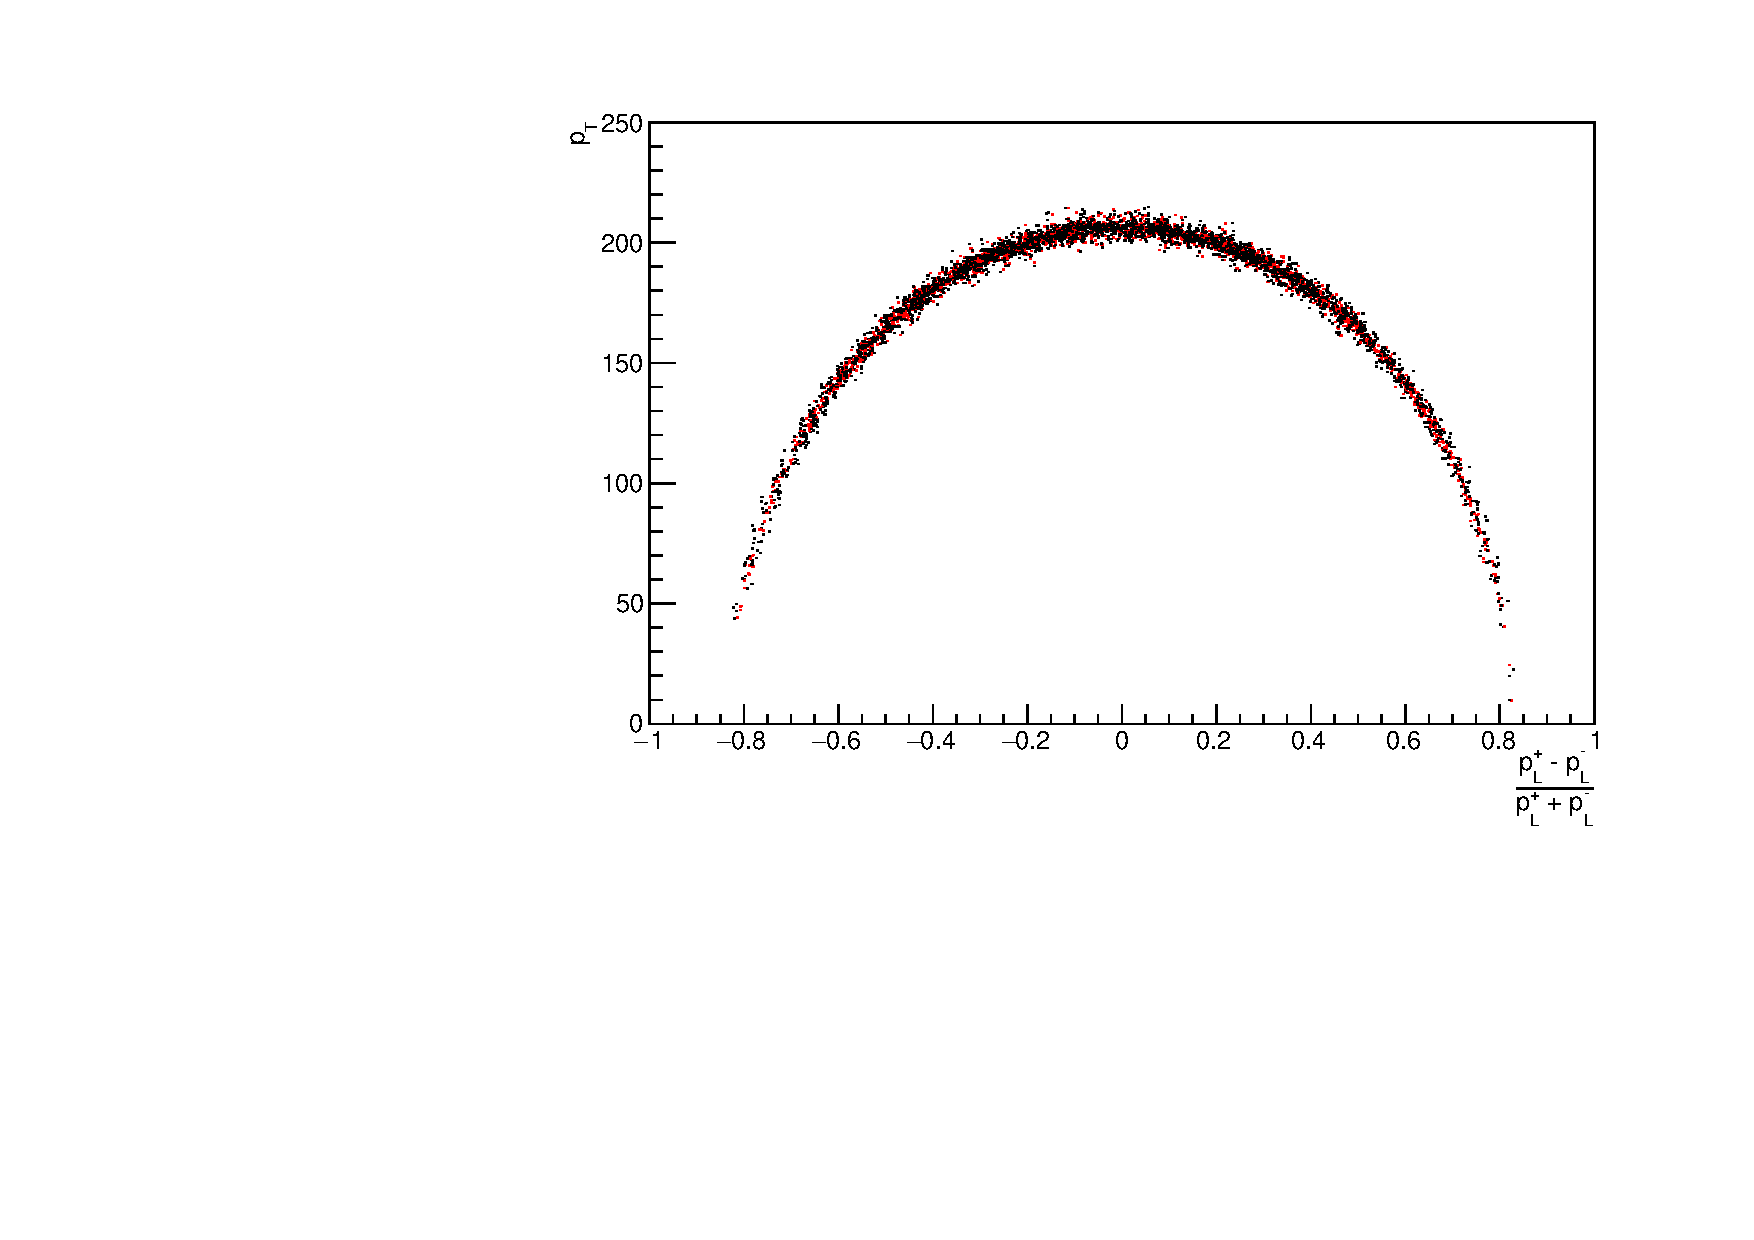
\includegraphics[width=0.5\linewidth]{figures/backgrounds/APplot_LL.pdf}
\put(-180,100) {(a)}
\hfill
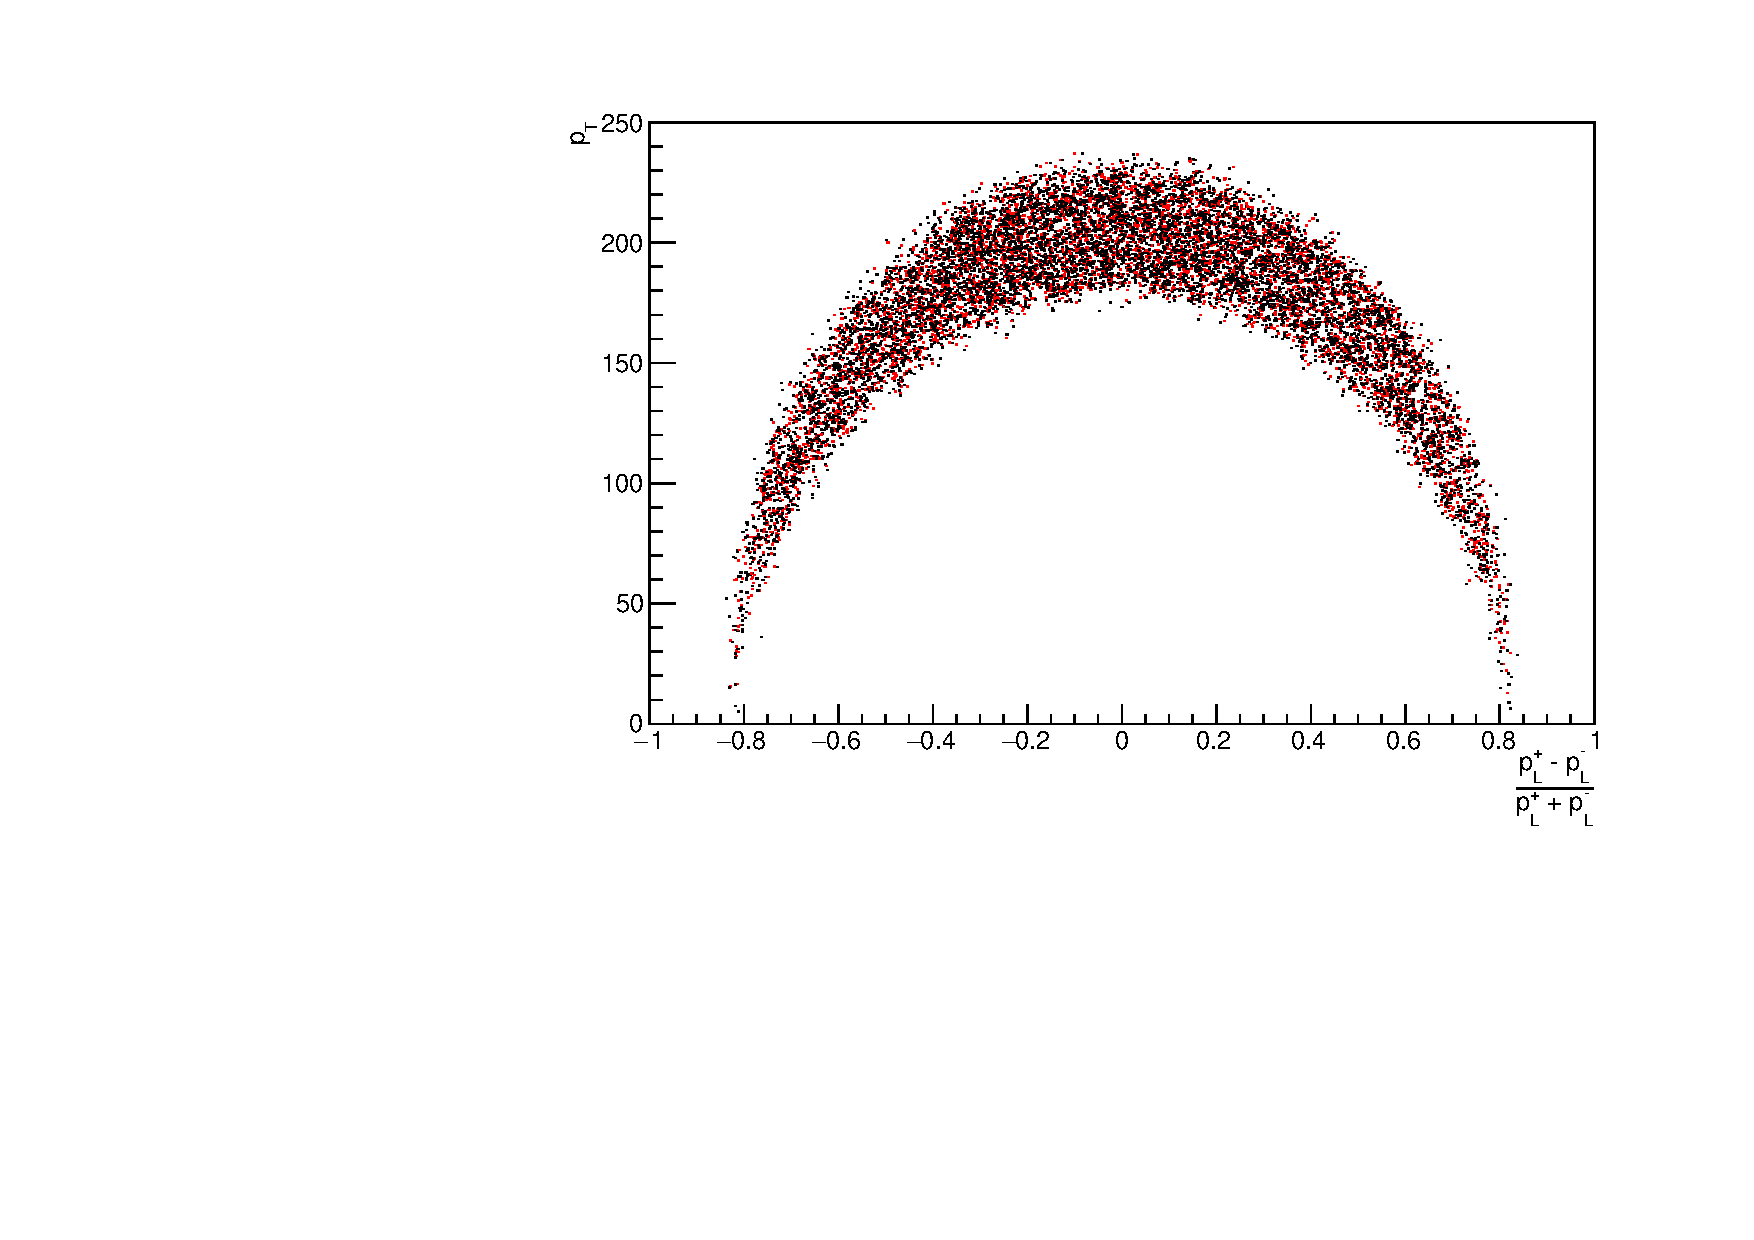
\includegraphics[width=0.5\linewidth]{figures/backgrounds/APplot_DD.pdf}
\put(-180,100) {(b)}
\caption{Armenteros-Podolanski plots for both data (black) and simulation (red) for (a) LL, and (b) DD candidates. The $p_T$ values on the $y$ axis are the transverse momentum of the daughters with respect to the mother particle and the $x$ axis is the longitudinal momentum asymmetry, defined in \eqn\ref{longitudinalpasy}.}
\label{applots}
\end{figure}


\subsubsection{\boldmath \decay{\B}{\D\KS\kaon} background}
\label{sec:backgrounds:b2dkks}

The decay \decay{\Bm}{\D\KS\Km} has a branching fraction of $5.5 \times 10^{-4}$~\cite{PDG2014}, which is similar to the signal \decay{\Bm}{\D\Kstarm(\KS\pim)} branching fraction. However, nearly all of this background is removed by the requirements that the reconstructed \Kstarm mass must be within 75 \mevcc of the known \Kstar mass and the DLLK of the bachelor pion must be less than four. This PID requirement suppresses the background by about 8\%. The efficiency of the \Kstarm mass selection when applied to the simulated \decay{\Bm}{\D\KS\Km} samples is 3\% for both LL and DD. This gives the expected contribution of \decay{\Bm}{\D\KS\Km} background in the \kpi mass spectrum to be less than 1\% of the signal, therefore the background is considered negligible. Any residual amount is investigated alongside the systematics for the residual low mass background in this region.

\subsection{Multivariate analysis with a Boosted Decision Tree}
\label{sec:selection:bdt}

Various selection requirements are placed on individual variables relating to particles in the decay chain in order to reduce specific background contributions. However, to achieve a much lower combinatorial background while retaining signal events requires more sophisticated classification techniques. As many variables are correlated with each other, the ability to separate signal from combinatorial background can be improved by using a multivariate analysis (MVA) method, which exploits correlations between the variables. 

The MVA implemented in this analysis is a Boosted Decision Tree (BDT)~\cite{Breiman}. Decision trees take a given set of variables from signal and background training samples and construct an algorithm to decide whether a given event corresponds to signal or background. Firstly, the best variable and value is found to split events into two subsets in order to maximise separation signal and background, the process is then repeated with a different variable for each of the two subsets. This is continuously repeated in order to build a tree, where the nodes at the end are called leaves. If more than half of the weight of a leaf corresponds to signal, it is a signal leaf, where each event is given a value of +1, otherwise it is a background leaf, where each event is given a value of -1. Signal events on a background leaf and background events on a signal leaf are misclassified. In order to stabilise this process, many trees are built to construct a weighted average over all the trees. After each tree is built, the misclassified events are reweighted (boosted) and a new tree is build with the reweighted events. The boosting makes misclassified events more likely to be correctly classified in future trees; a particular type of boosting, called gradient boost, is used in this analysis. The result of the process assigns each event a weight from -1 (most background-like) to +1 (most signal-like). 

\subsubsection{Training samples}

A BDT with the gradient boost (BDTG) method using the Toolkit for Multivariate Analysis (TMVA) framework~\cite{TMVA} is employed in order to reduce the combinatorial background level. A separate BDT is trained for LL and DD candidates, named BDTG\_LL and BDTG\_DD respectively. The BDTs are mainly based on topological variables, so are insensitive as to whether the \Dz daughters are kaons or pions. Therefore, the same BDT is used for all of the two-body \Dz decay modes, trained using \kpi decays, and another BDT is used for all the four-body \Dz decay modes, trained using \kpipipi decays. 

For the two body modes, simulated samples for the decay \kpi are used to provide a signal sample. Events from data in the favoured \kpi mode in the region of \Bm mass above 5600 MeV are used as a sample of background combinatorial events. Generation of simulated events is computationally expensive. A small simulated sample is produced from full \lhcb simulation in order to determine efficiencies. The sample is small due to the mode being very low efficiency, so many generated events fail the reconstruction. However, BDT training requires a significantly larger sample, and the available resources are insufficient to simply generate more events. A work-around is employed to remove events, which are less likely to pass the selection, at generator level. Events are removed on the basis of low momentum or transverse momentum of signal tracks or intermediate particles. This reduces the number of events required to be simulated in the \lhcb detector, which is the most computationally expensive part of the reconstruction process. The advantage of this approach is that 89\% of generated events are removed, significantly reducing the resource requirement. However, the disadvantage is that the selection has to be more stringent than the final selection and 20\% of events that would have passed are removed. Therefore, the BDT may not be as optimal as it may have been with unlimited resources, however this trade-off is deemed acceptable given the BDTs high performance, as discussed later in this section.

For \kpipipi, signal samples of simulated events for the decay without any selection requirements at generator level are used. This is possible due to an artifact of the time that each stage of the analysis was performed; at this later time the resource availability improved. Events from data in the favoured \kpipipi mode in the region of \Bm mass above 5600 MeV are used as a sample of background combinatorial events. All samples used in training the BDTs are split into a training and testing sample before being used as an input to the multivariate algorithm.

\subsubsection{Setup and implementation of the multivariate algorithm}

Initial selection requirements are applied to both the signal and background training samples to remove candidates that would not pass the final selection. This allows a more accurate discrimination between signal and background in data. The selection criteria on the training samples are:

\begin{itemize}
\item The \chisq of the decay chain refit per degree of freedom, $\chisq_\text{refit}$, must lie between 0 and 100,
\item The \chisqip of the \Bm candidate, with respect to the \Bm vertex, must lie between 0 and 25,
\item The reconstructed \Kstarm mass must lie within 500~\mevcc of the known \Kstarm mass,
\item The reconstructed \KS mass must lie with 15~\mevcc of the known \KS mass for LL candidates and 20~\mevcc for DD candidates.
\end{itemize}
These selection requirements are looser than those applied to the full selection, discussed in \sect\ref{sec:selection:strippingandtrigger}. For example, here no requirement is imposed on the reconstructed \Dz mass and the \Kstarm mass requirement is as wide as 500\mevcc rather than the 75\mevcc used in the full selection. This is because the training samples required for the BDT must be large enough for the multivariate algorithm to distinguish between important differences in the signal and background samples rather than statistical fluctuations in the distributions. Imposing a tighter selection is found to reduce the size of the samples to a point where the BDTs would be sub-optimal.

Various input variables are used to exploit the topologies of the two- and four-body decays. Of particular importance are the $\chisq_\text{refit}$ and the $p_T$ asymmetry between the \Bm candidate and other tracks from the same PV, defined as
\begin{equation}
A_{\pt} = \frac{p_T^B - p_T^{\text{cone}}}{p_T^B + p_T^{\text{cone}}} \text{ ,}
\label{ptasy}
\end{equation}
where $p_T^B$ is the $p_T$ of the reconstructed \Bm signal candidate and $p_T^{\text{cone}}$ is the sum of the $p_T$ of all other tracks in a cone of radius 1.50 surrounding the \Bm candidate. This is a quantitative measure of the isolation of the \Bm candidate. Some of the variables are transformed using a logarithm function to increase their separation power. Other input variables used include the logarithm of the \chisqip for the \Bm, bachelor, \Dz and all the \Dz decay products, the logarithm of the \chisqip for the \KS and both its decay products (for LL only) and the $p_T$ of the \KS candidate (for DD candidates only). The variables used in the BDT are slightly different for LL and DD candidates since the separation power of the \KS variables significantly differs between these samples. 

Tables~\ref{BDTinputvariables2body} and \ref{BDTinputvariables4body} show the list of input variables in the two and four-body BDTs respectively, ranked by separation power. The distributions of the two-body BDT input variables in the signal and background training samples are shown in Figs.~\ref{BDTinputdist2bodyLL} and \ref{BDTinputdist2bodyDD}. The equivalent distributions of the input variables for the four-body BDT are similar. Other variables and different setups of testing and training samples were investigated but found to have negligible improvement.

\begin{table}
\centering
\subfloat[Input variables for the two-body BDTs.][Input variables for the two-body BDTs.]{
\begin{tabular}{lll}
Rank & Variable in BDT\_LL & Variable in BDT\_DD \\
\hline
1 & log($\chisq_\text{refit}$) & log($\chisq_\text{refit}$) \\
2 & log(\KS \chisqip) & log(\Dz daughter kaon \chisqip) \\
3 & log(max \KS daughter \chisqip) & log(Bachelor \chisqip) \\
4 & $A_{\pt}$ & $A_{\pt}$ \\
5 & log(\Dz daughter kaon \chisqip) & log(\Dz daughter pion \chisqip) \\
6 & log(Bachelor \chisqip) & log(\Dz \chisqip) \\
7 & log(\Dz \chisqip) & log(\Bm \chisqip) \\
8 & log(min \KS daughter \chisqip) & \KS $p_T$ \\
9 & log(\Dz daughter pion \chisqip) & - \\
10 & log(\Bm \chisqip) & - \\
\end{tabular}
\label{BDTinputvariables2body}}
%\caption{Ranking for variables for BDTG\_LL and BDTG\_DD for the two-body BDTs.}
%\label{BDTinputvariables2body}
\qquad
\subfloat[Input variables for the four-body BDTs.][Input variables for the four-body BDTs.]{
\begin{tabular}{lll}
Rank & Variable in BDT\_LL & Variable in BDT\_DD \\
\hline
1 & log($\chisq_\text{refit}$) & log($\chisq_\text{refit}$) \\
2 & log(\KS \chisqip) & $A_{\pt}$ \\
3 & $A_{\pt}$ & log(\Bm \chisqip) \\
4 & log(\Bm \chisqip) & log(Bachelor \chisqip) \\
5 & log(\Dz \chisqip) & \KS $p_T$ \\
6 & log(\Dz daughter kaon \chisqip) & log(\Dz \chisqip) \\
7 & log(Bachelor \chisqip) & log(max \Dz daughter \chisqip) \\
8 & log(min \Dz daughter \chisqip) & log(\Dz daughter ss \chisqip) \\
9 & log(max \KS daughter \chisqip) & log(\Dz daughter kaon \chisqip) \\
10 & log(\Dz daughter ss \chisqip) & log(min \Dz daughter \chisqip) \\
11 & log(min \KS daughter \chisqip) & - \\
12 & log(max \Dz daughter \chisqip) & - \\
\end{tabular}
\label{BDTinputvariables4body}}
\caption{List of input variables for the (a) two-body, and (b) four-body, BDTs, ranked by separation power. The variable $A_{\pt}$ represents the \pt asymmetry as defined in \eqn~\ref{ptasy} and ``max (min) \KS daughter \chisqip'' refers to the \chisqip of the \KS daughter which has the largest (smallest) \chisqip. For the four-body BDTs, the particle name ``D daughter ss'' refers to the pion from the \Dz meson which has the same sign of the kaon.}
\end{table}

\begin{figure}
\centering
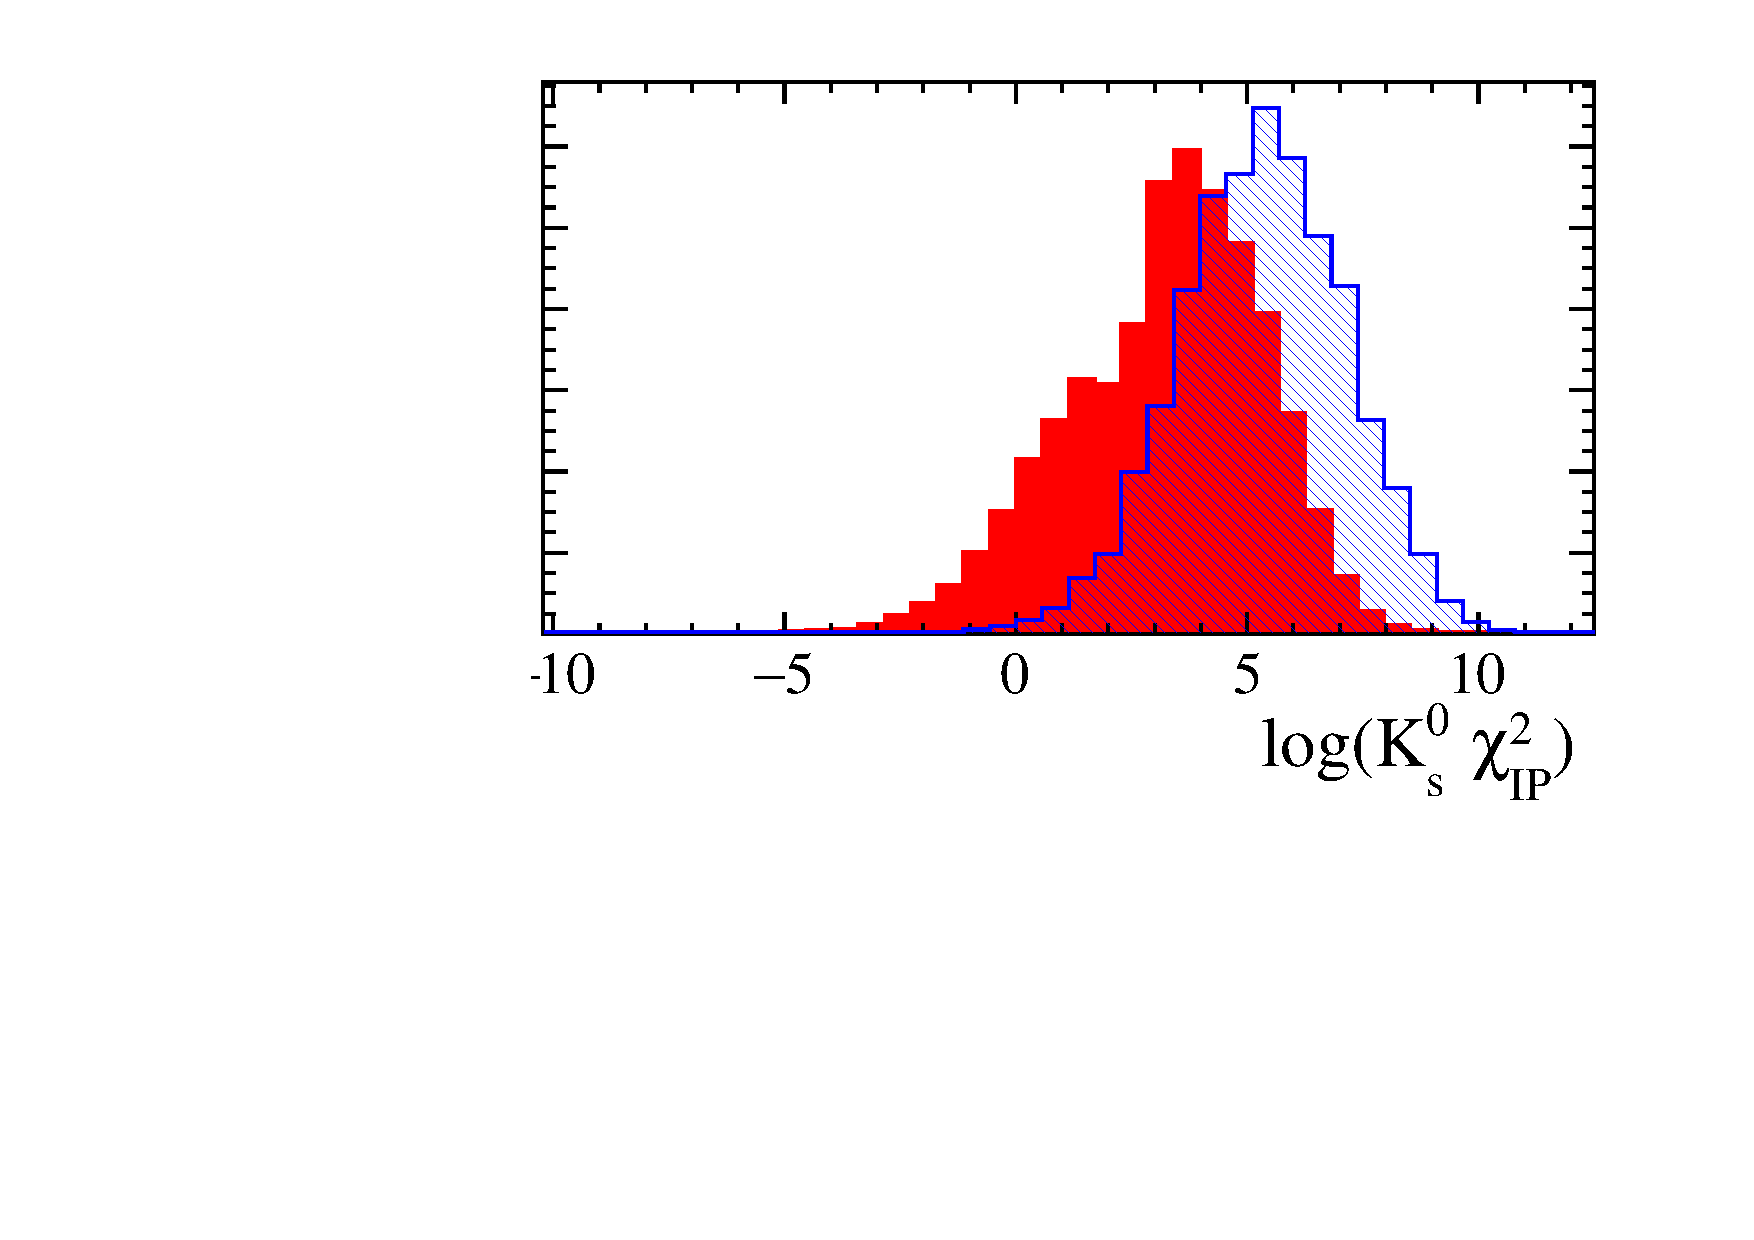
\includegraphics[width=0.3\linewidth]{figures/selection/BDTvariables/BDT_Var_KPi_LL_log_Ks_IPCHI2_OWNPV_.pdf}
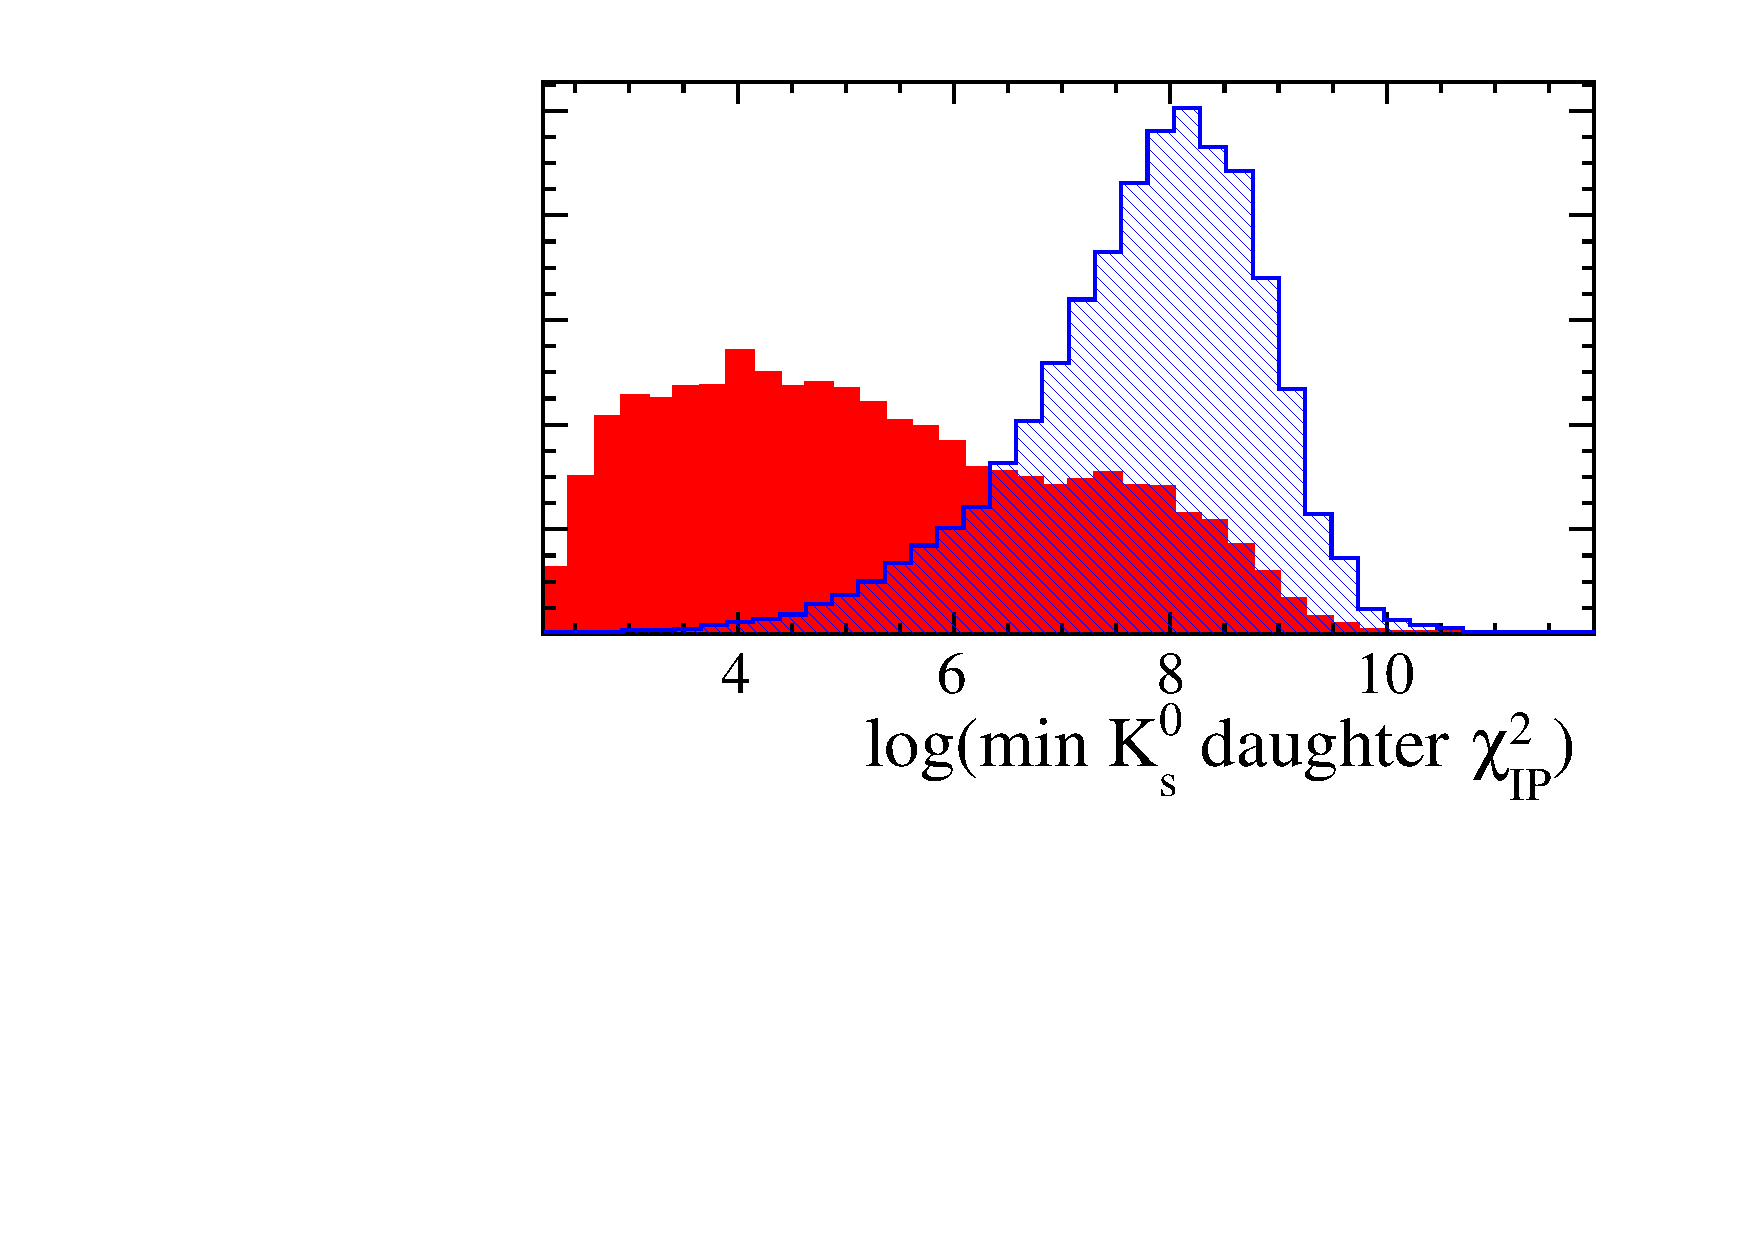
\includegraphics[width=0.3\linewidth]{figures/selection/BDTvariables/BDT_Var_KPi_LL_log_max_Ksh_IPCHI2_OWNPV_.pdf}
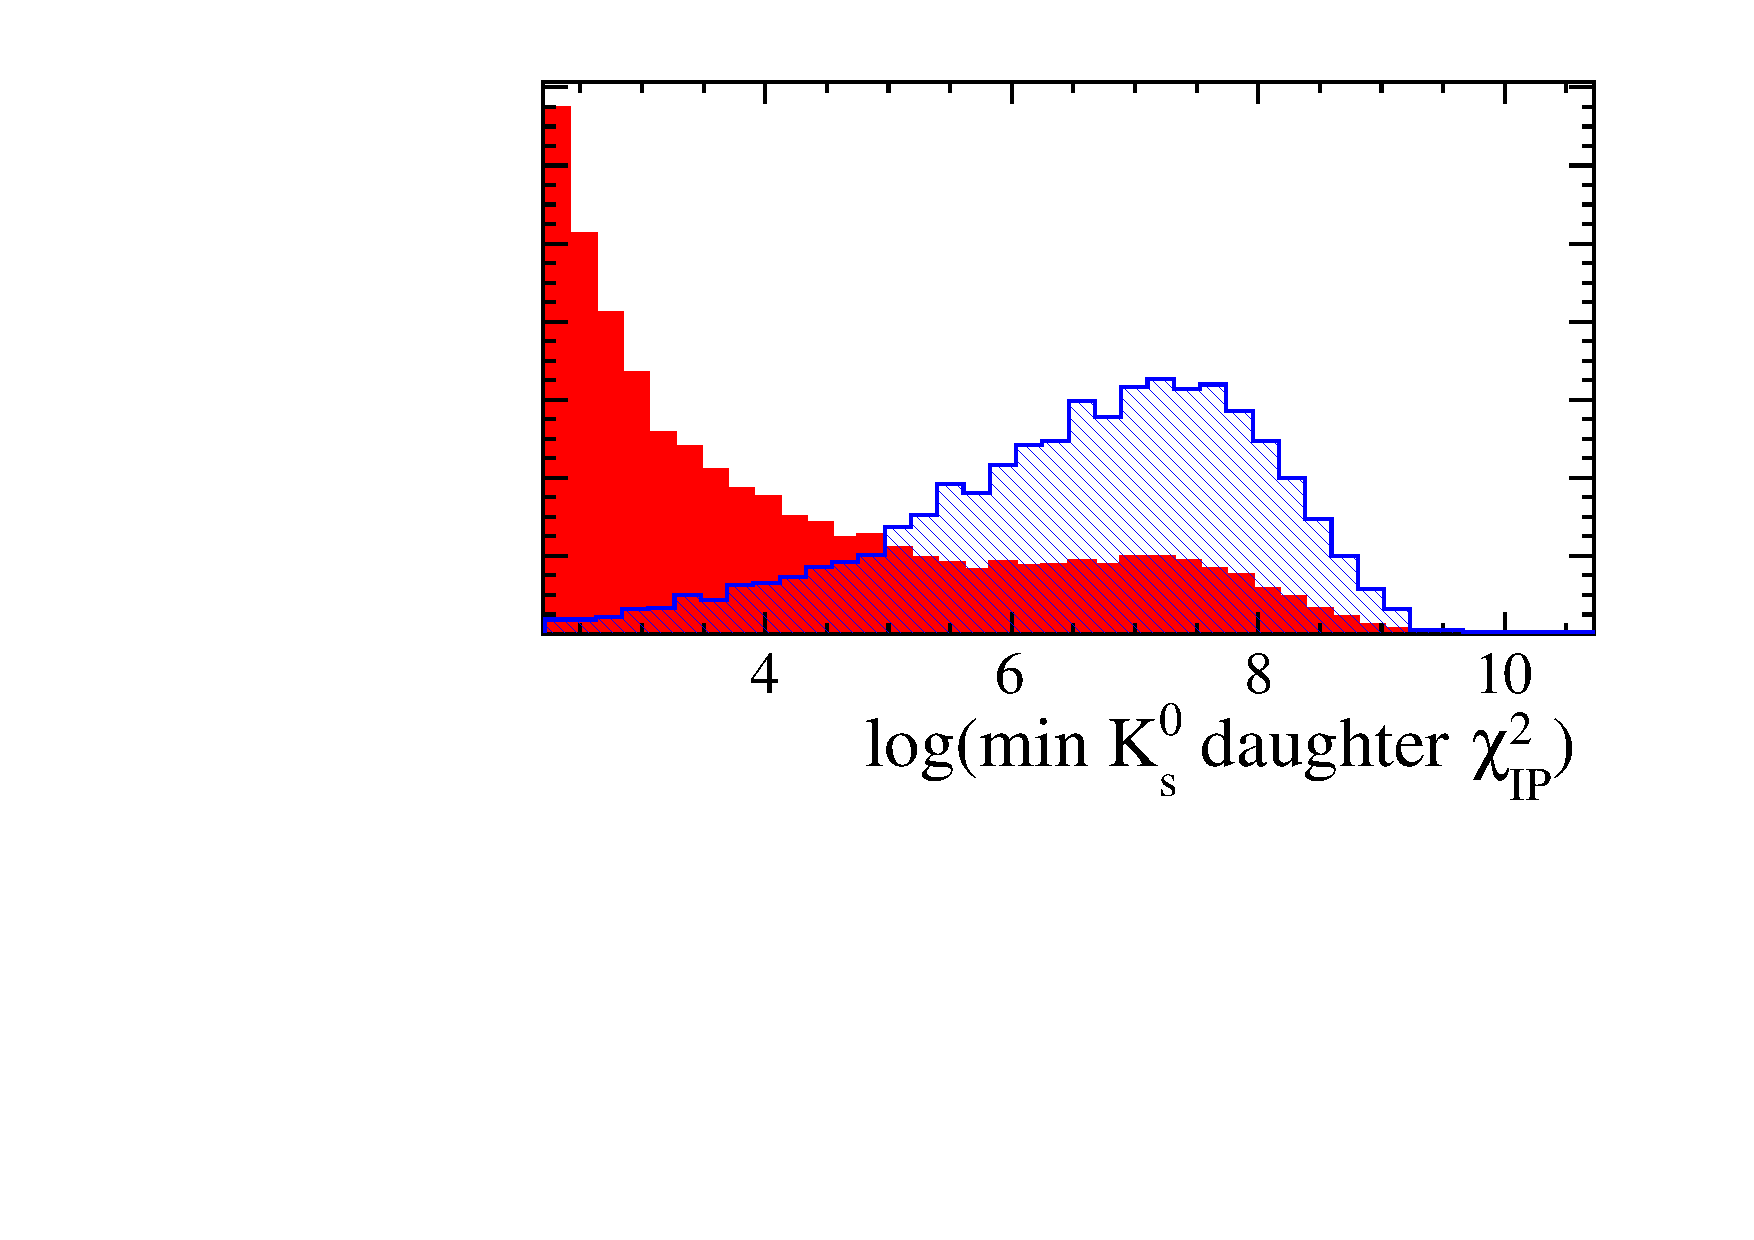
\includegraphics[width=0.3\linewidth]{figures/selection/BDTvariables/BDT_Var_KPi_LL_log_min_Ksh_IPCHI2_OWNPV_.pdf}
\hfill
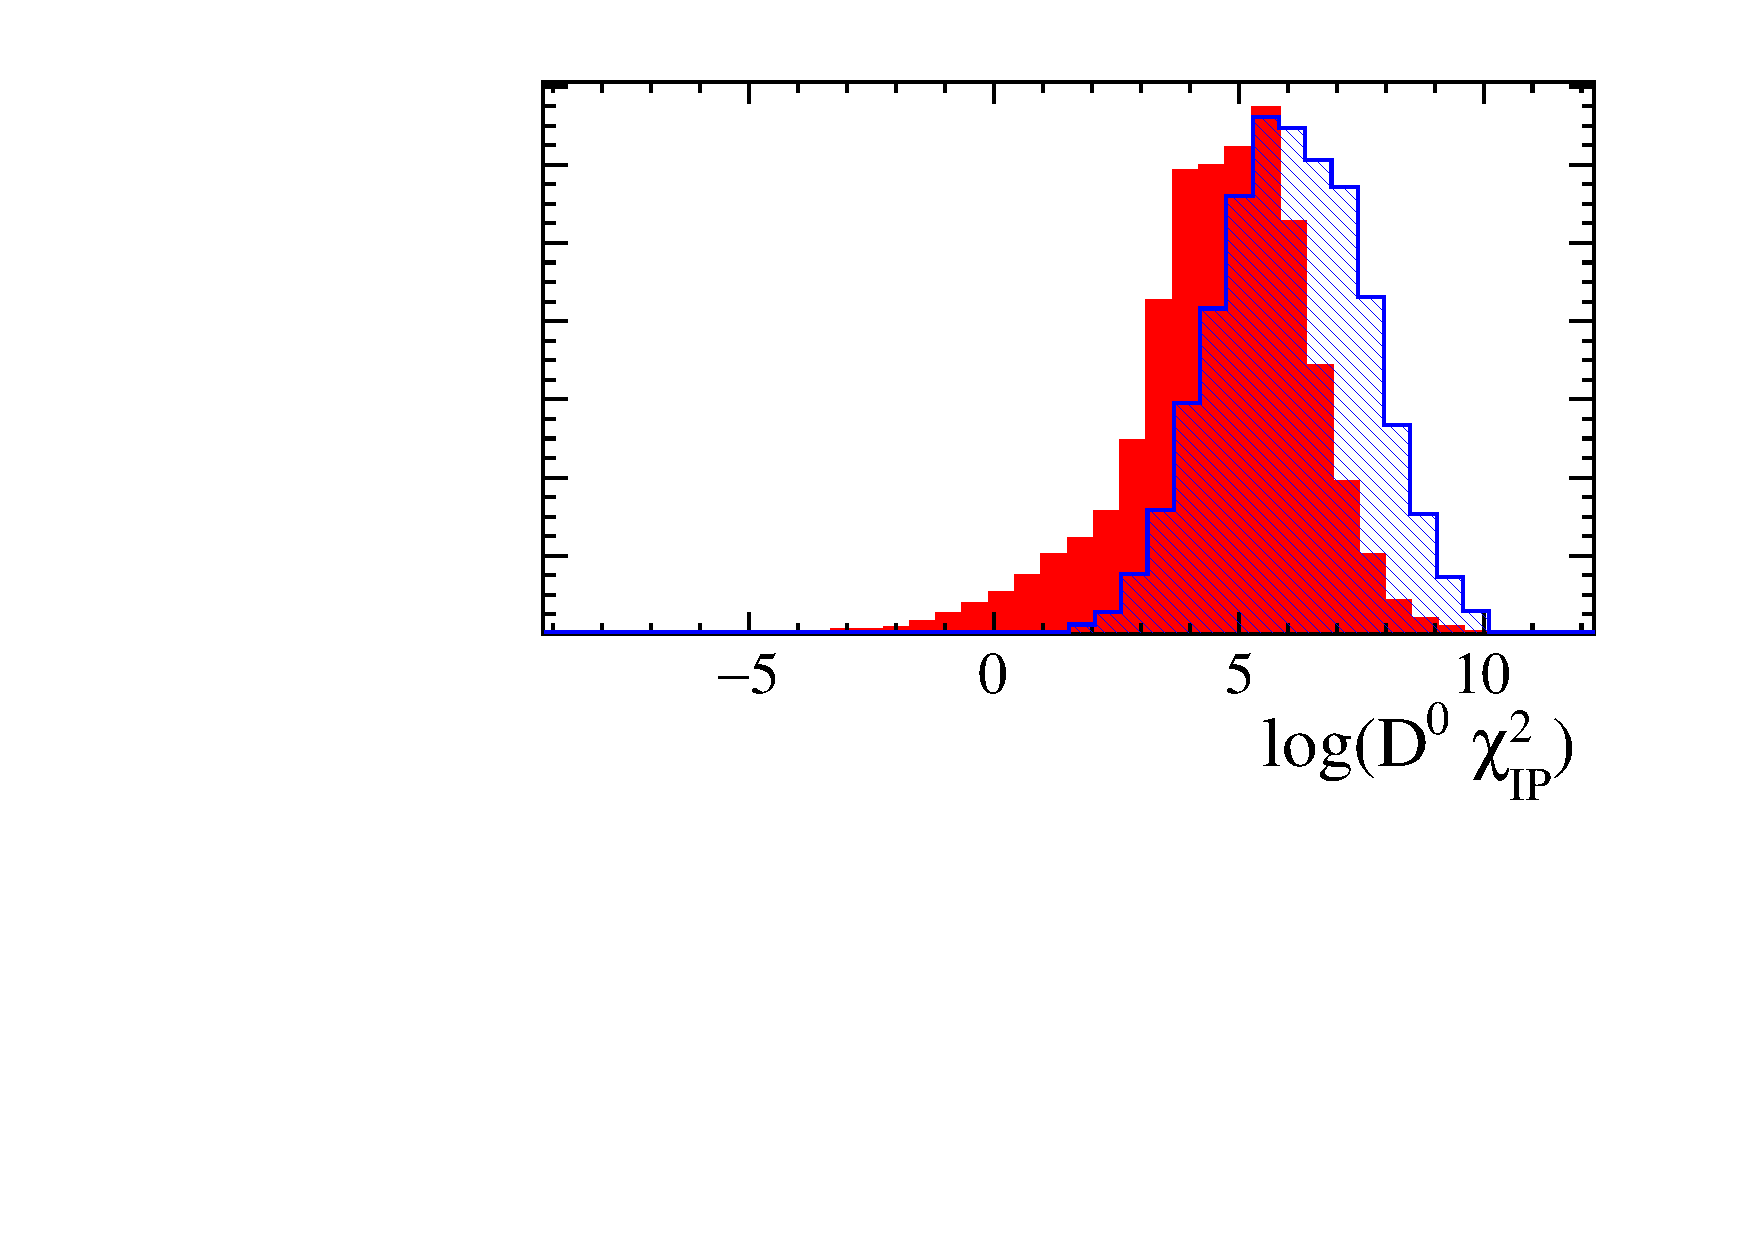
\includegraphics[width=0.3\linewidth]{figures/selection/BDTvariables/BDT_Var_KPi_LL_log_D0_IPCHI2_OWNPV_.pdf}
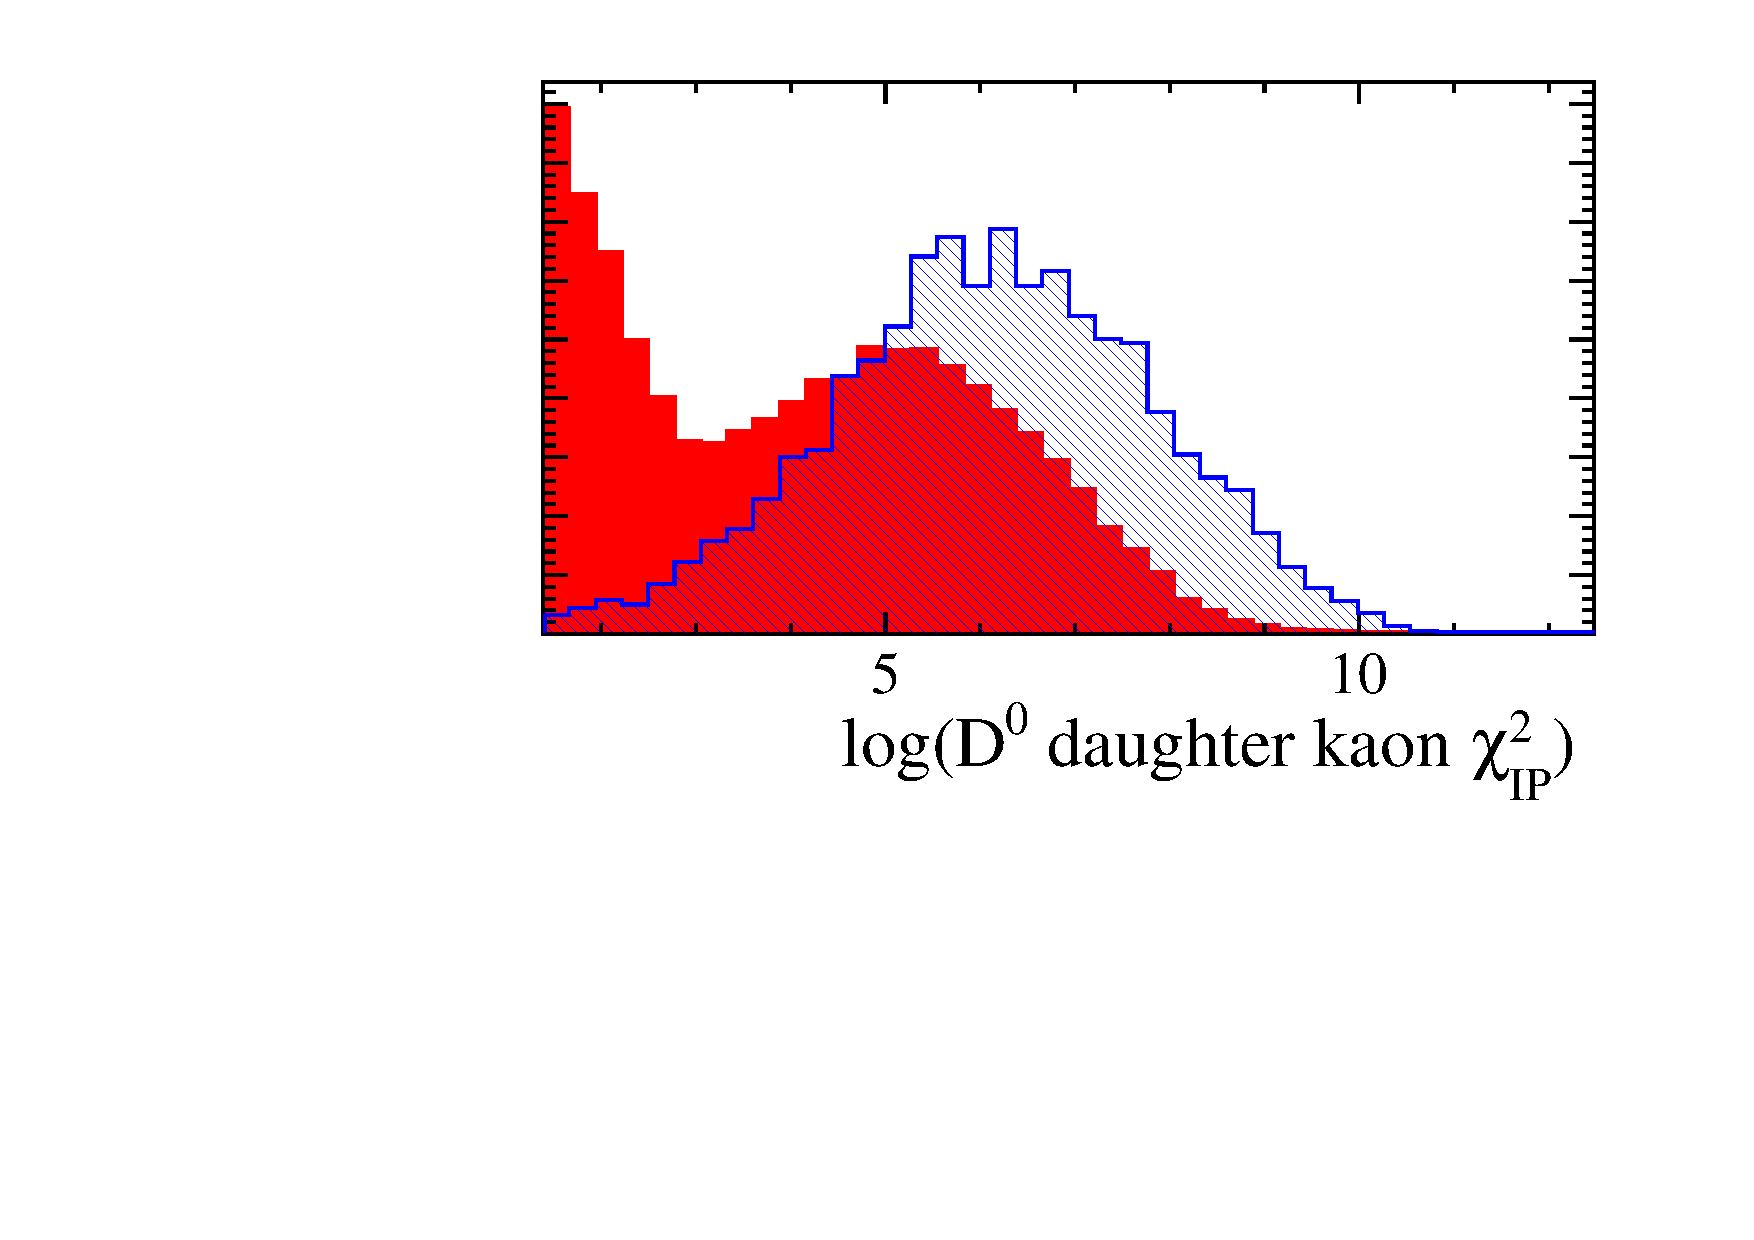
\includegraphics[width=0.3\linewidth]{figures/selection/BDTvariables/BDT_Var_KPi_LL_log_Dh1_IPCHI2_OWNPV_.pdf}
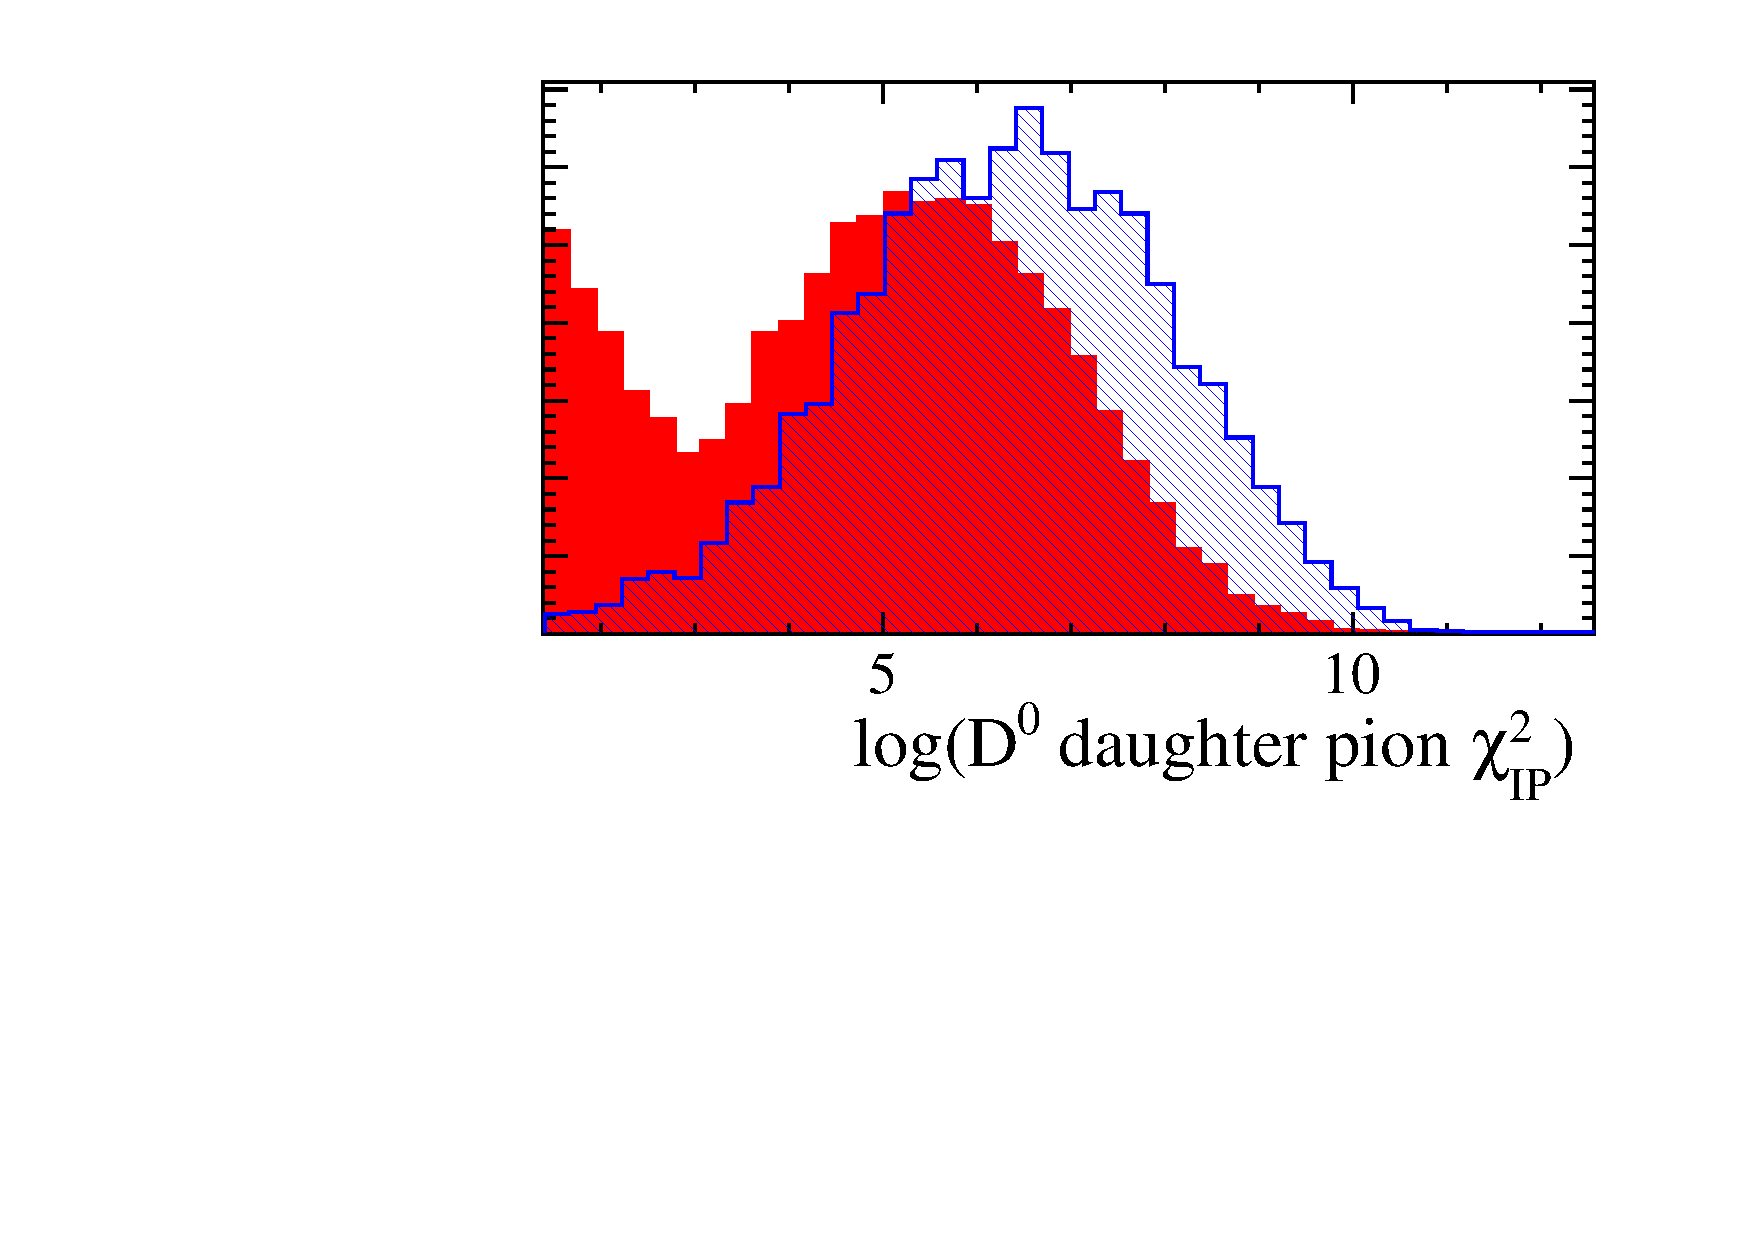
\includegraphics[width=0.3\linewidth]{figures/selection/BDTvariables/BDT_Var_KPi_LL_log_Dh2_IPCHI2_OWNPV_.pdf}
\hfill
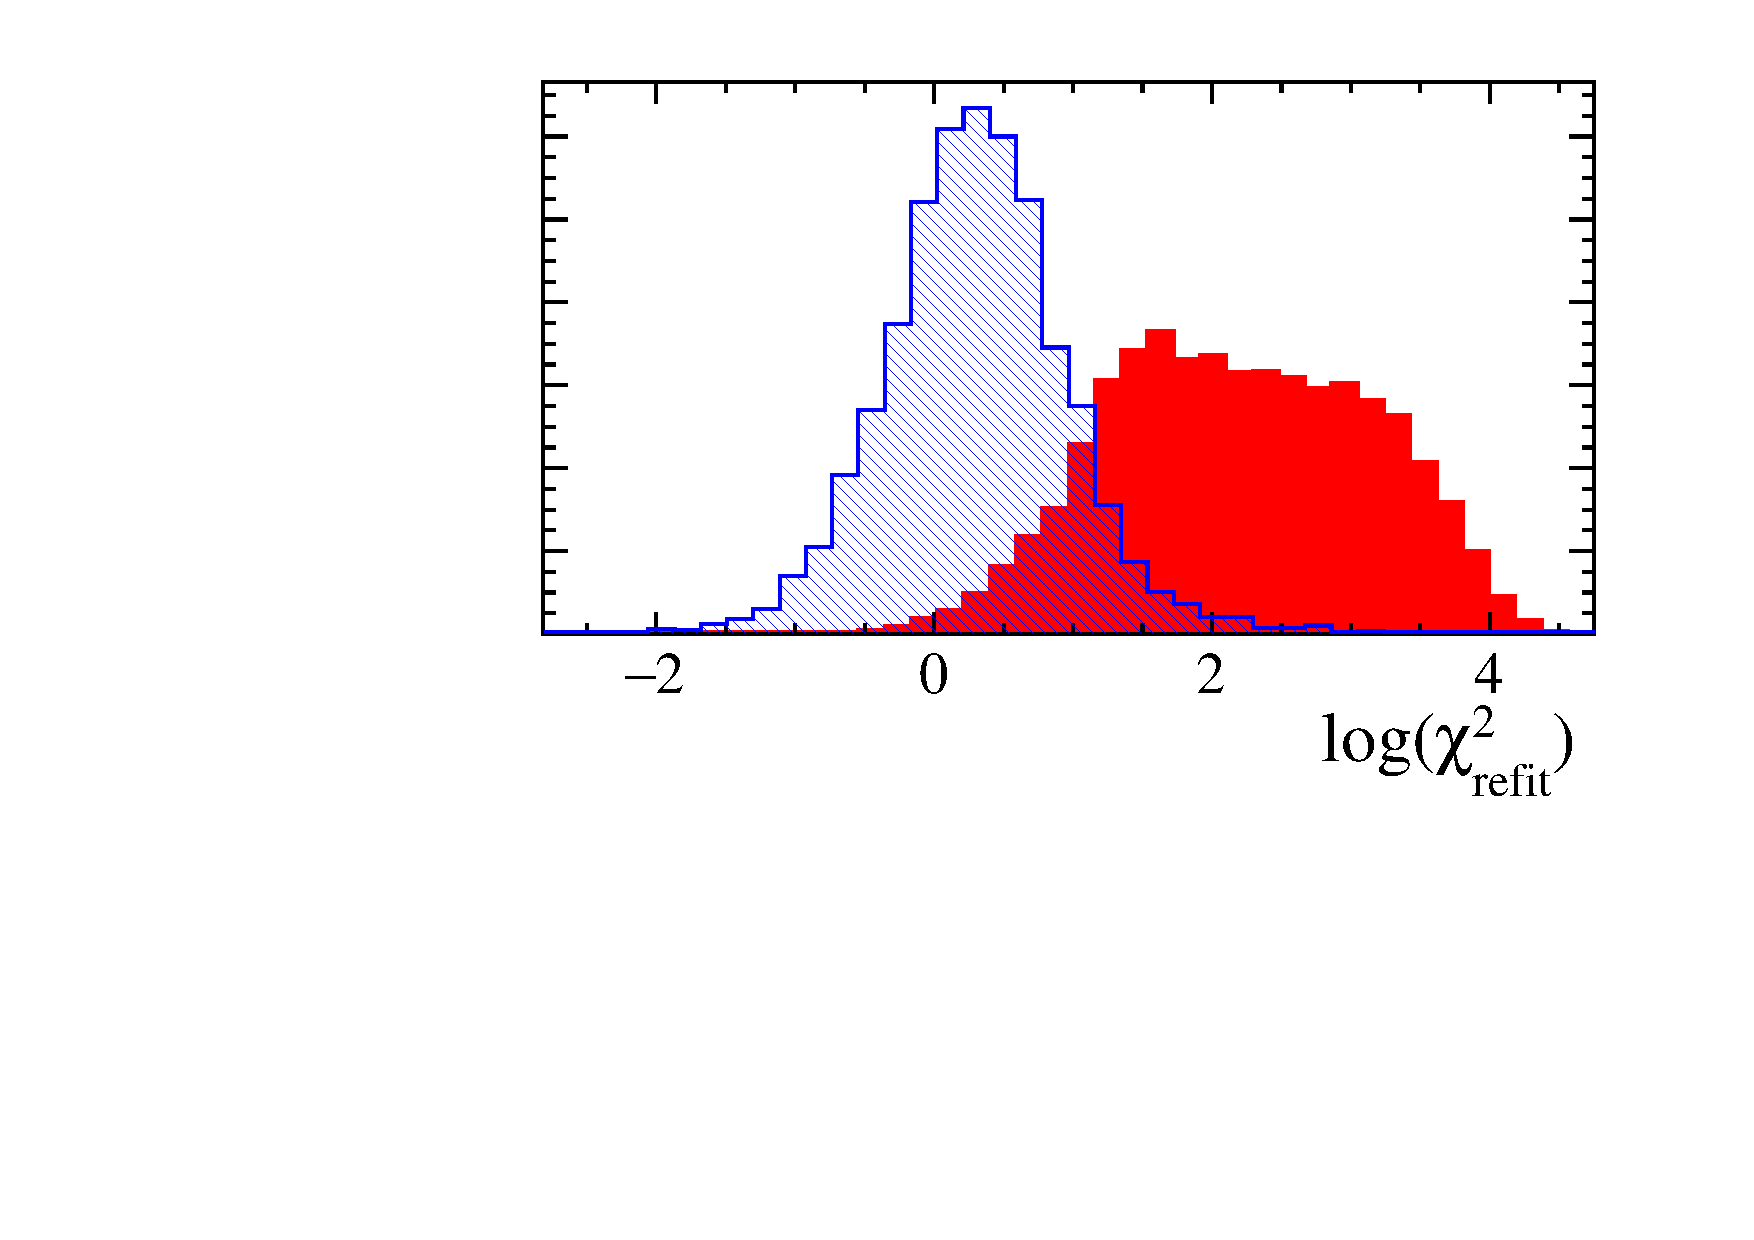
\includegraphics[width=0.3\linewidth]{figures/selection/BDTvariables/BDT_Var_KPi_LL_log_Bu_D0constKS0constPVconst_CHI2NDOF_.pdf}
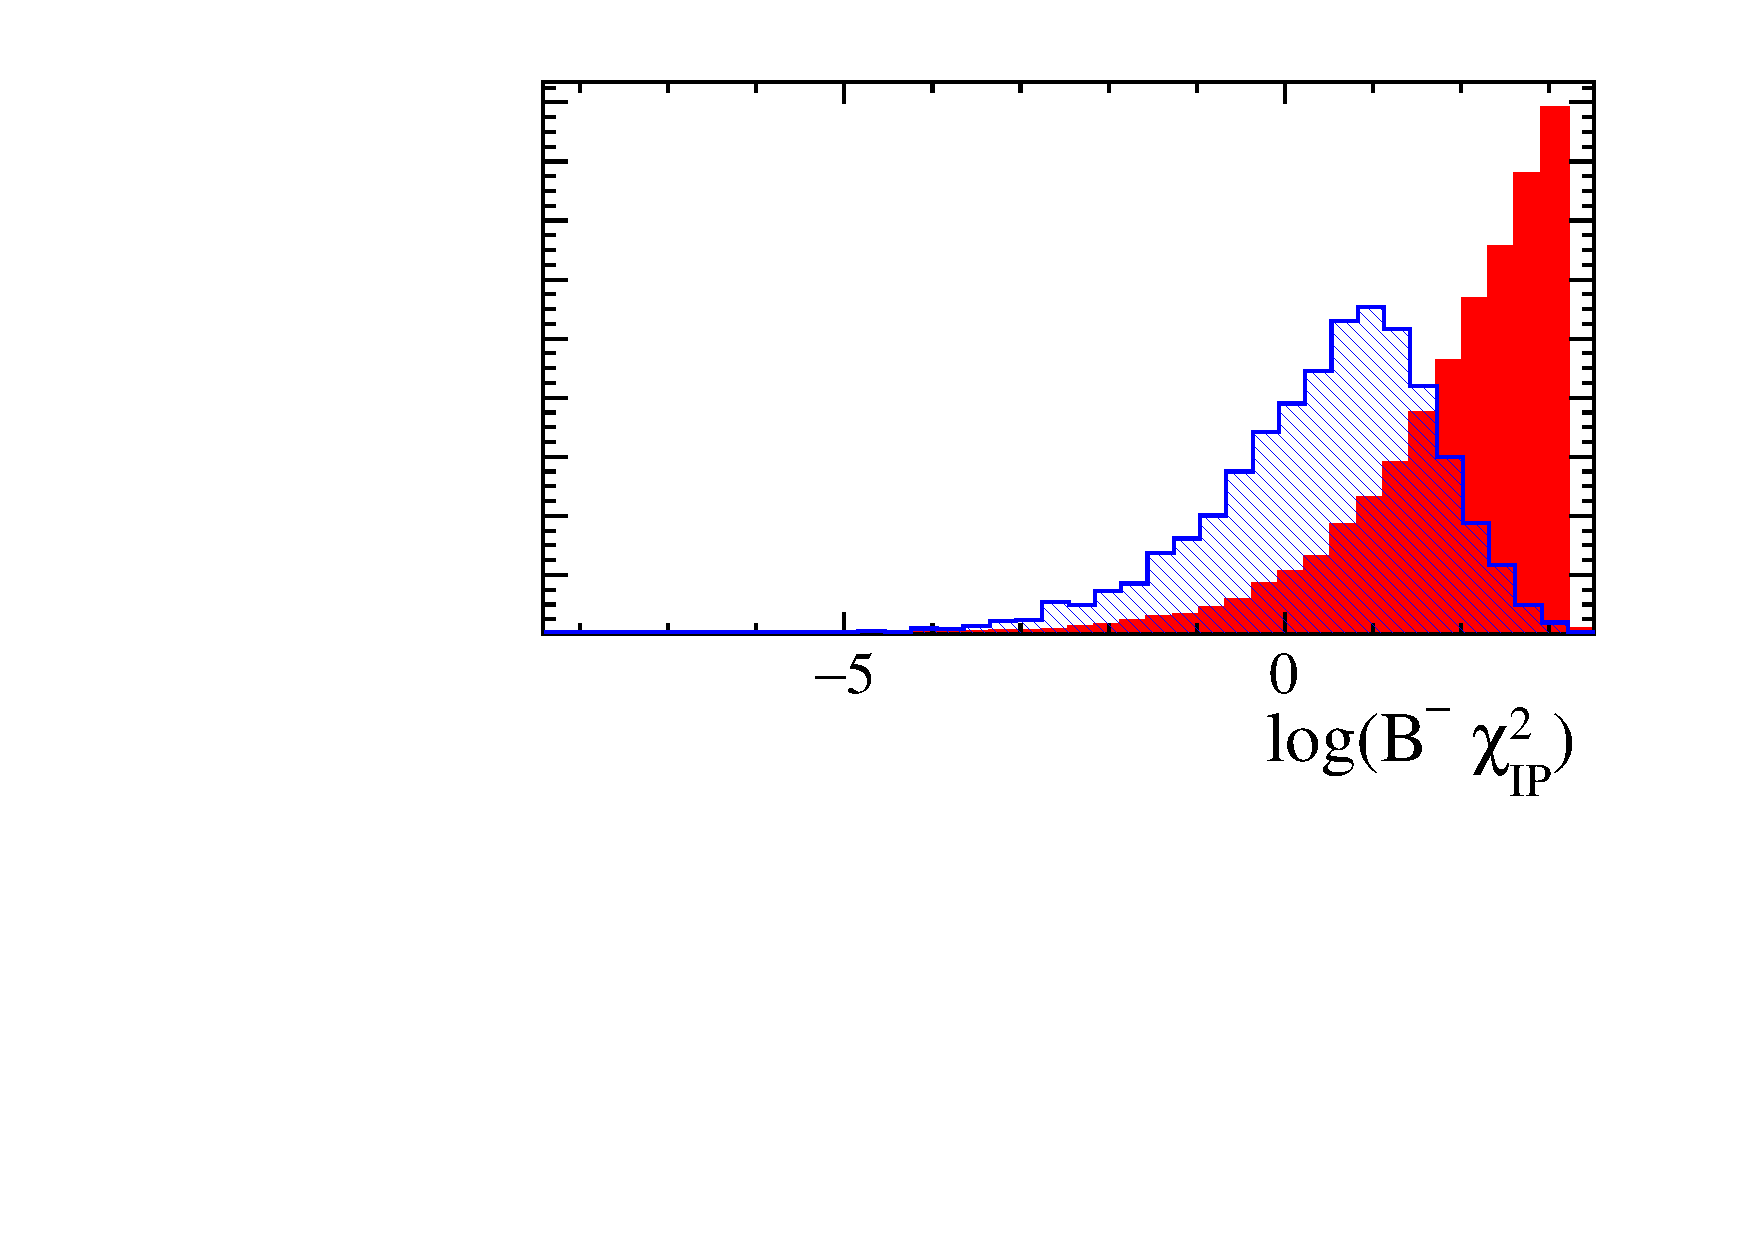
\includegraphics[width=0.3\linewidth]{figures/selection/BDTvariables/BDT_Var_KPi_LL_log_Bu_IPCHI2_OWNPV_.pdf}
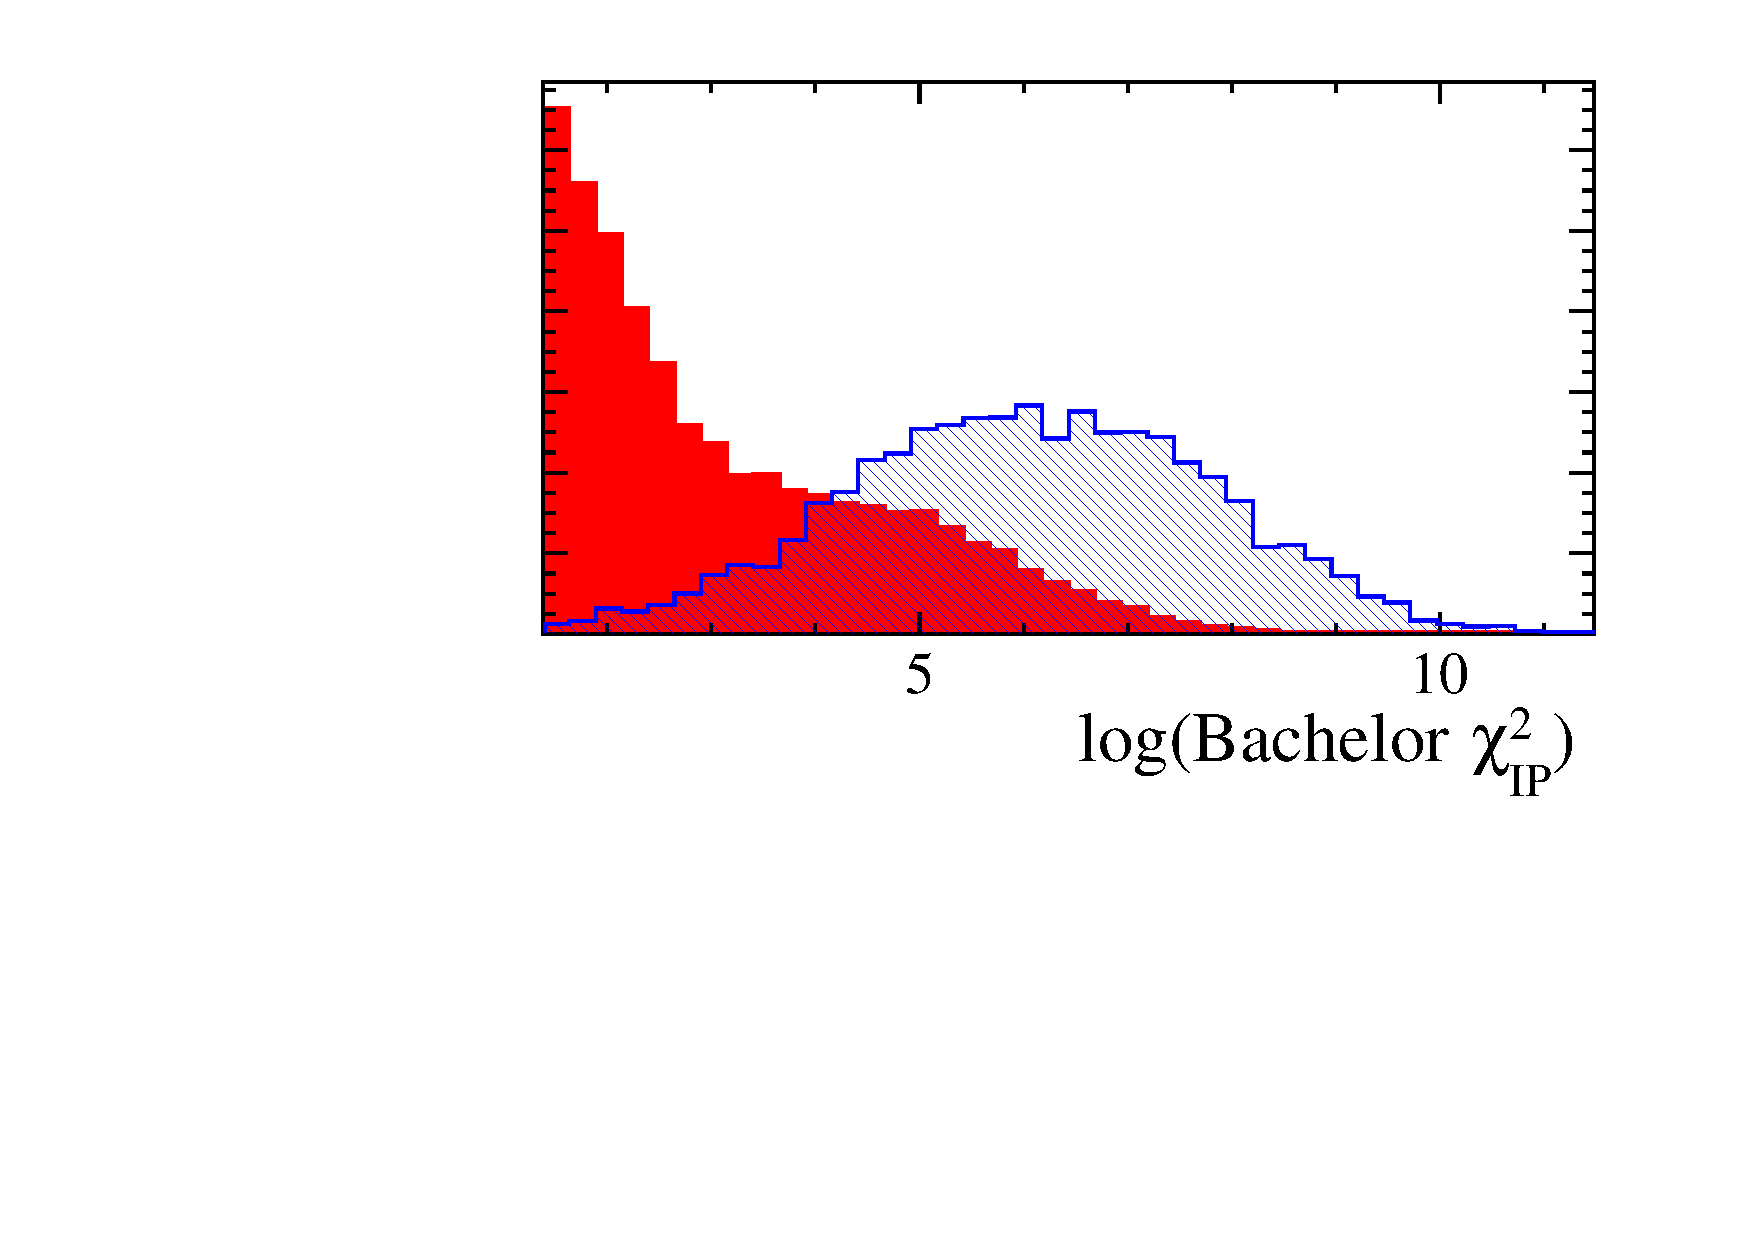
\includegraphics[width=0.3\linewidth]{figures/selection/BDTvariables/BDT_Var_KPi_LL_log_Bach_IPCHI2_OWNPV_.pdf}
\hfill
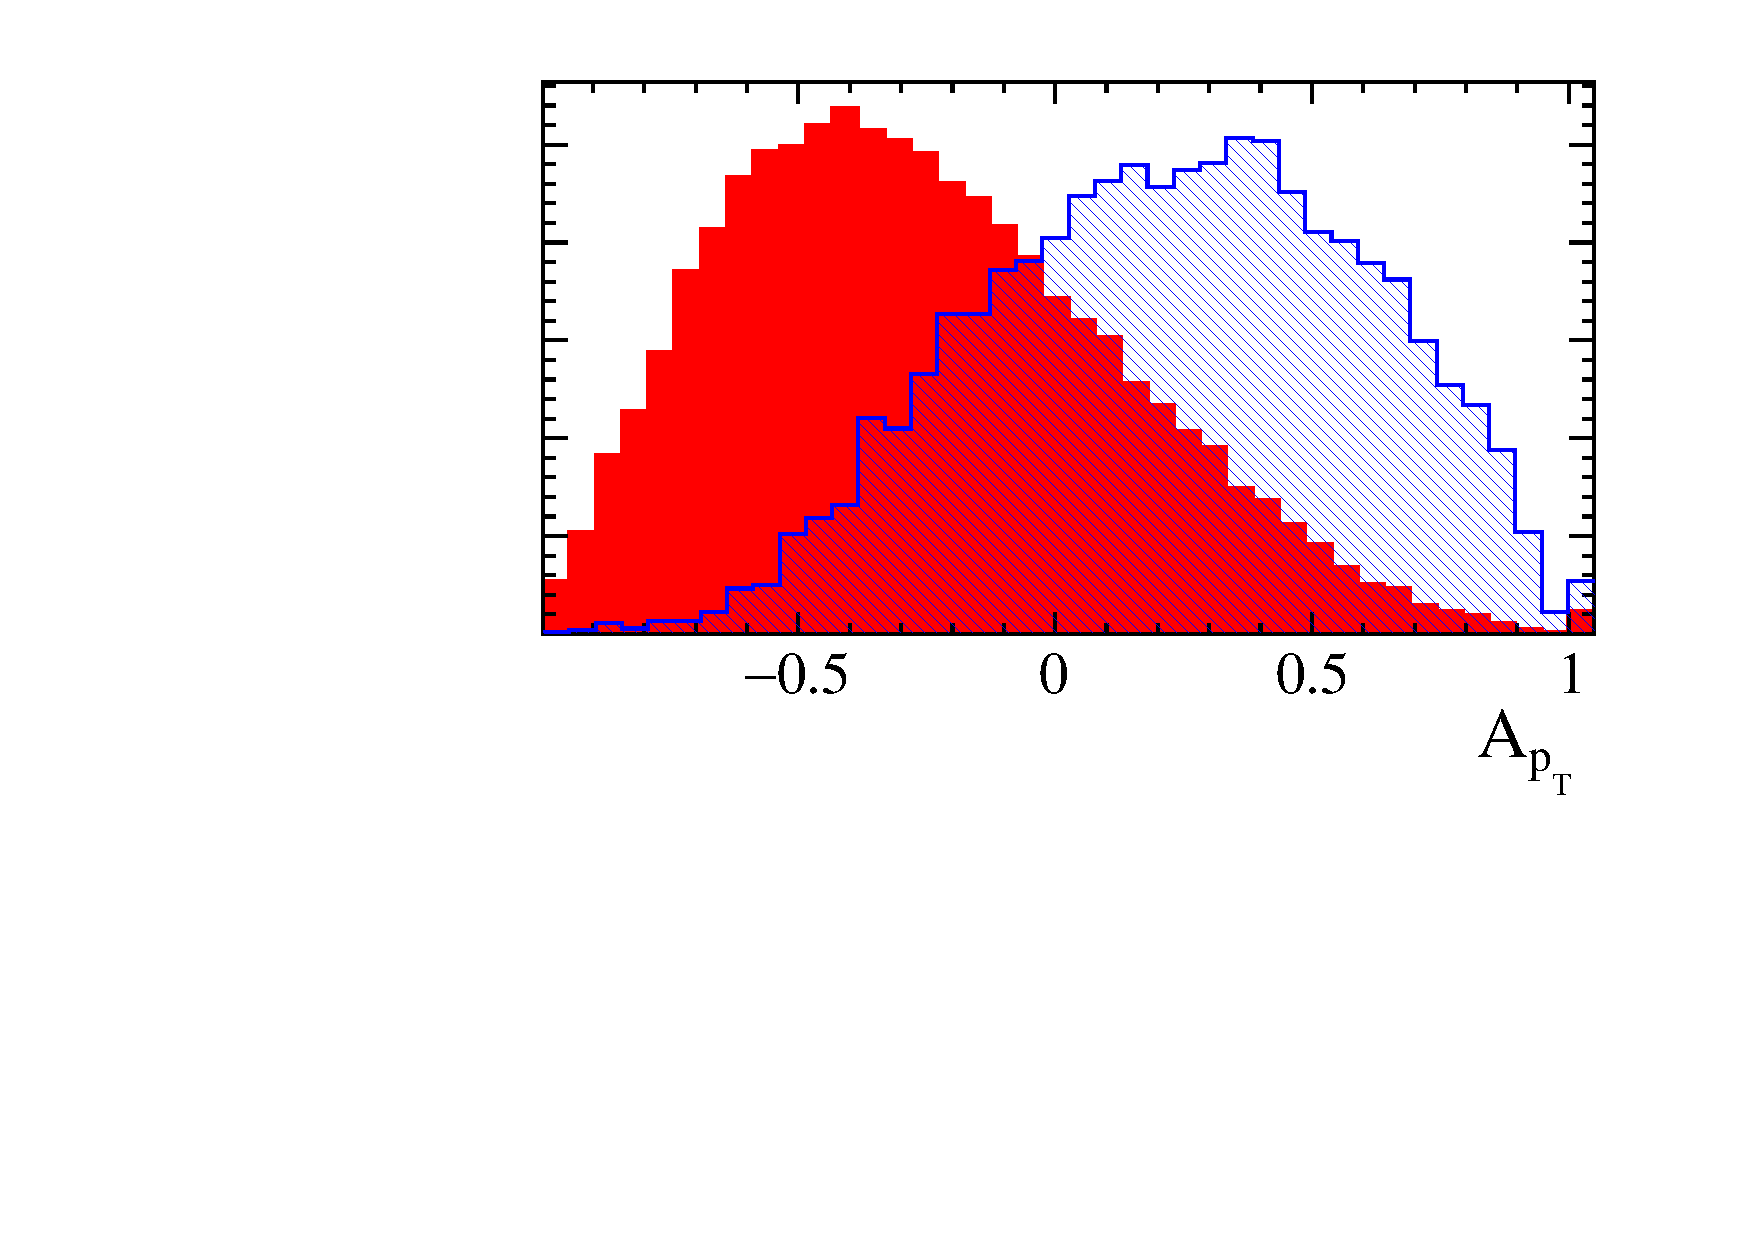
\includegraphics[width=0.3\linewidth]{{figures/selection/BDTvariables/BDT_Var_KPi_LL_Bu_ptasy_1.50}.pdf}
\caption{Distributions of the input variables using the signal (blue) and background (red) training samples for the two-body LL BDT. The variable $A_{\pt}$ represents the \pt asymmetry as defined in \eqn~\ref{ptasy} and ``max (min) \KS daughter \chisqip'' refers to the \chisqip of the \KS daughter which has the largest (smallest) \chisqip. All distributions have been normalised to unity in order to easily compare their shape, therefore the vertical axis is not labelled as it is not of interest here.}
\label{BDTinputdist2bodyLL}
\end{figure}

\begin{figure}
\centering
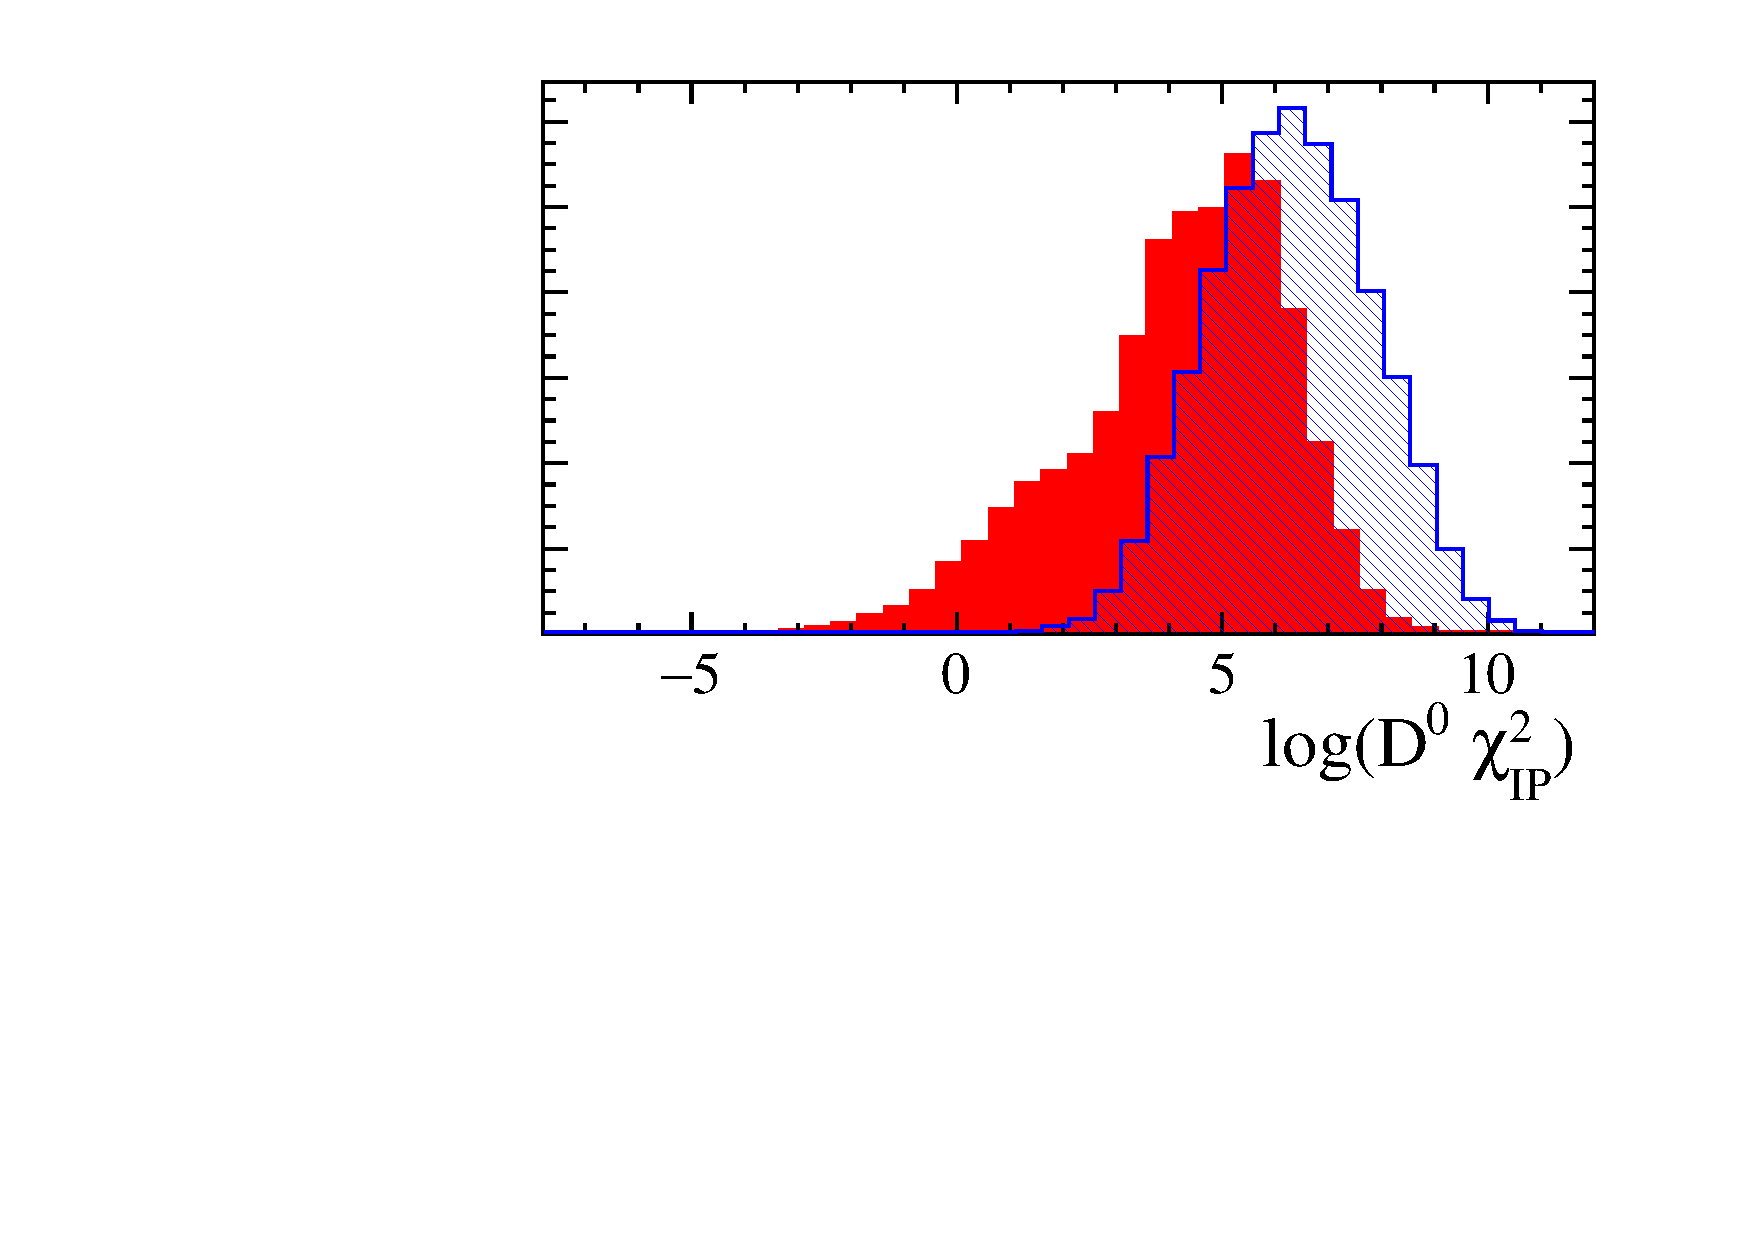
\includegraphics[width=0.3\linewidth]{figures/selection/BDTvariables/BDT_Var_KPi_DD_log_D0_IPCHI2_OWNPV_.pdf}
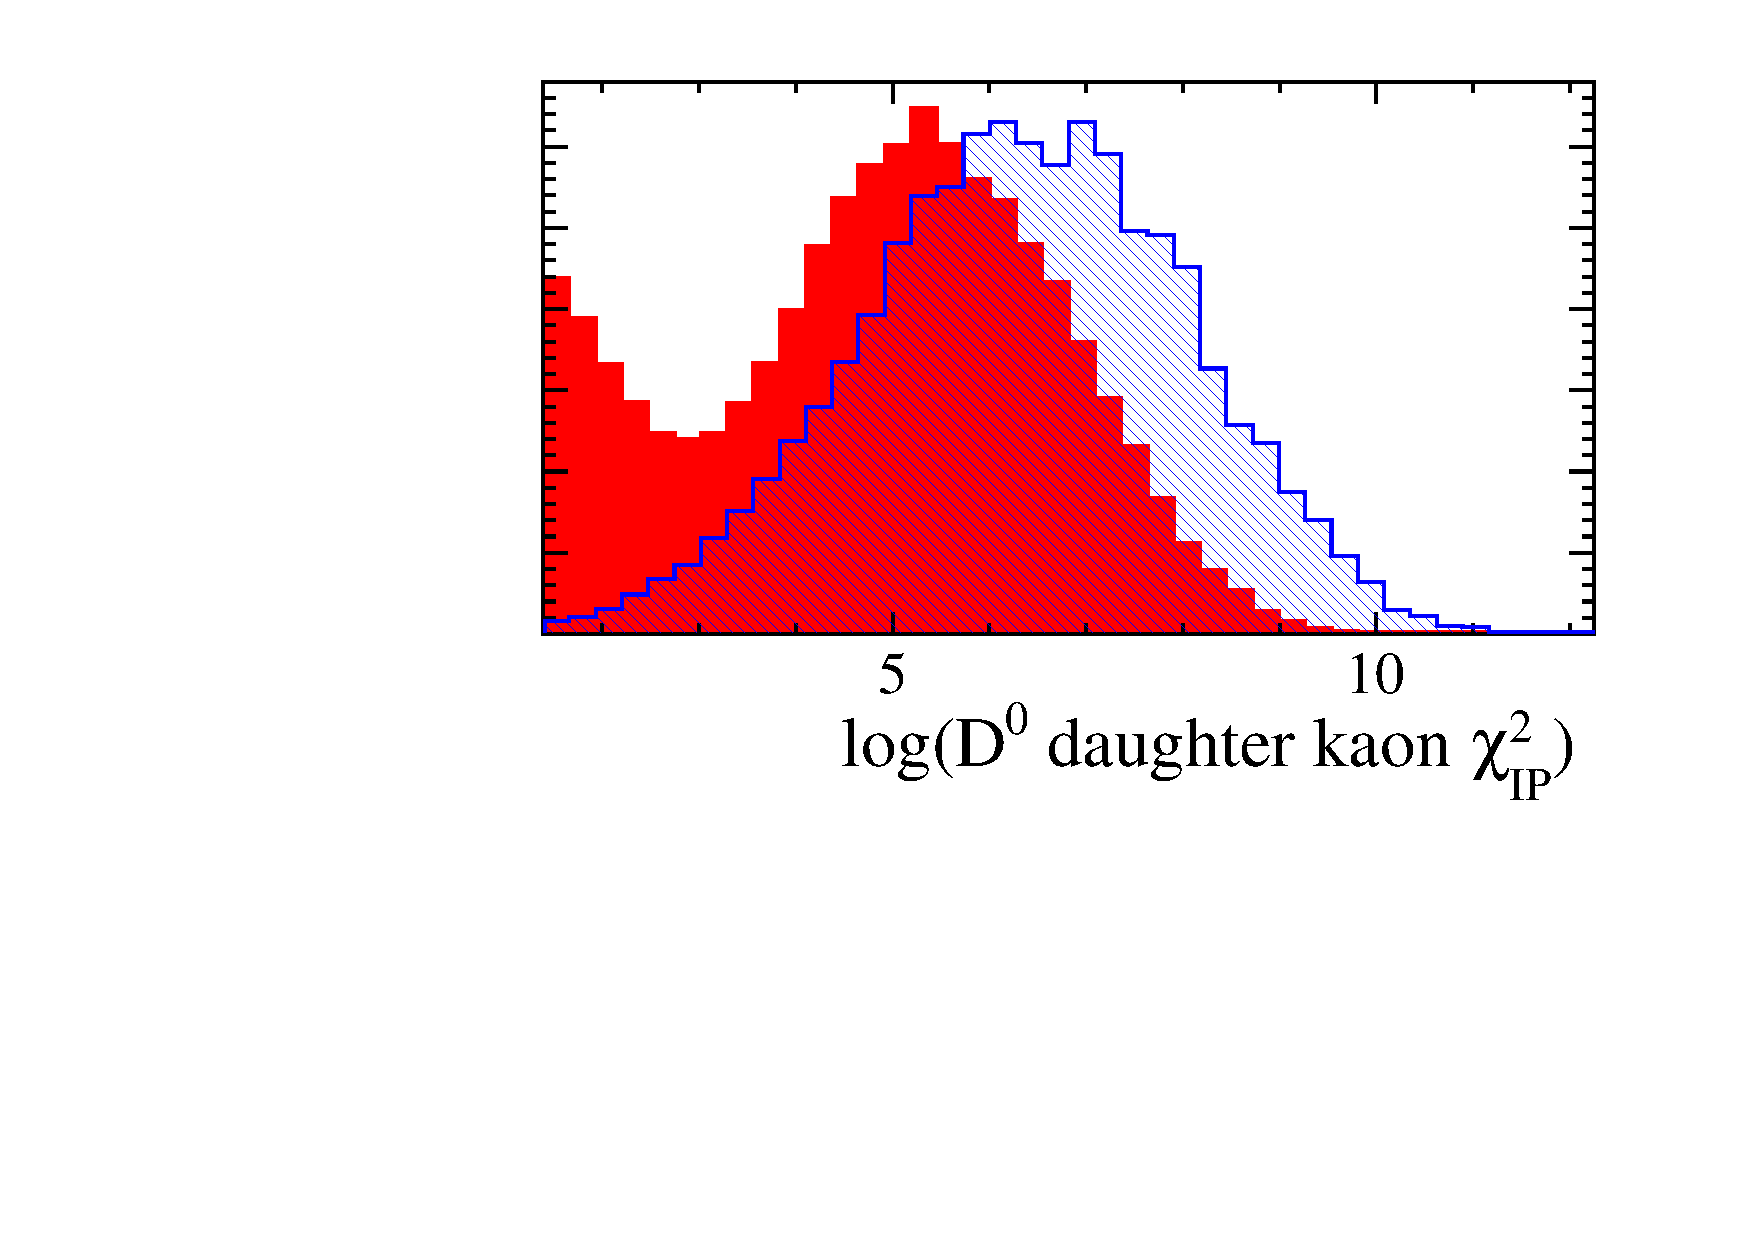
\includegraphics[width=0.3\linewidth]{figures/selection/BDTvariables/BDT_Var_KPi_DD_log_Dh1_IPCHI2_OWNPV_.pdf}
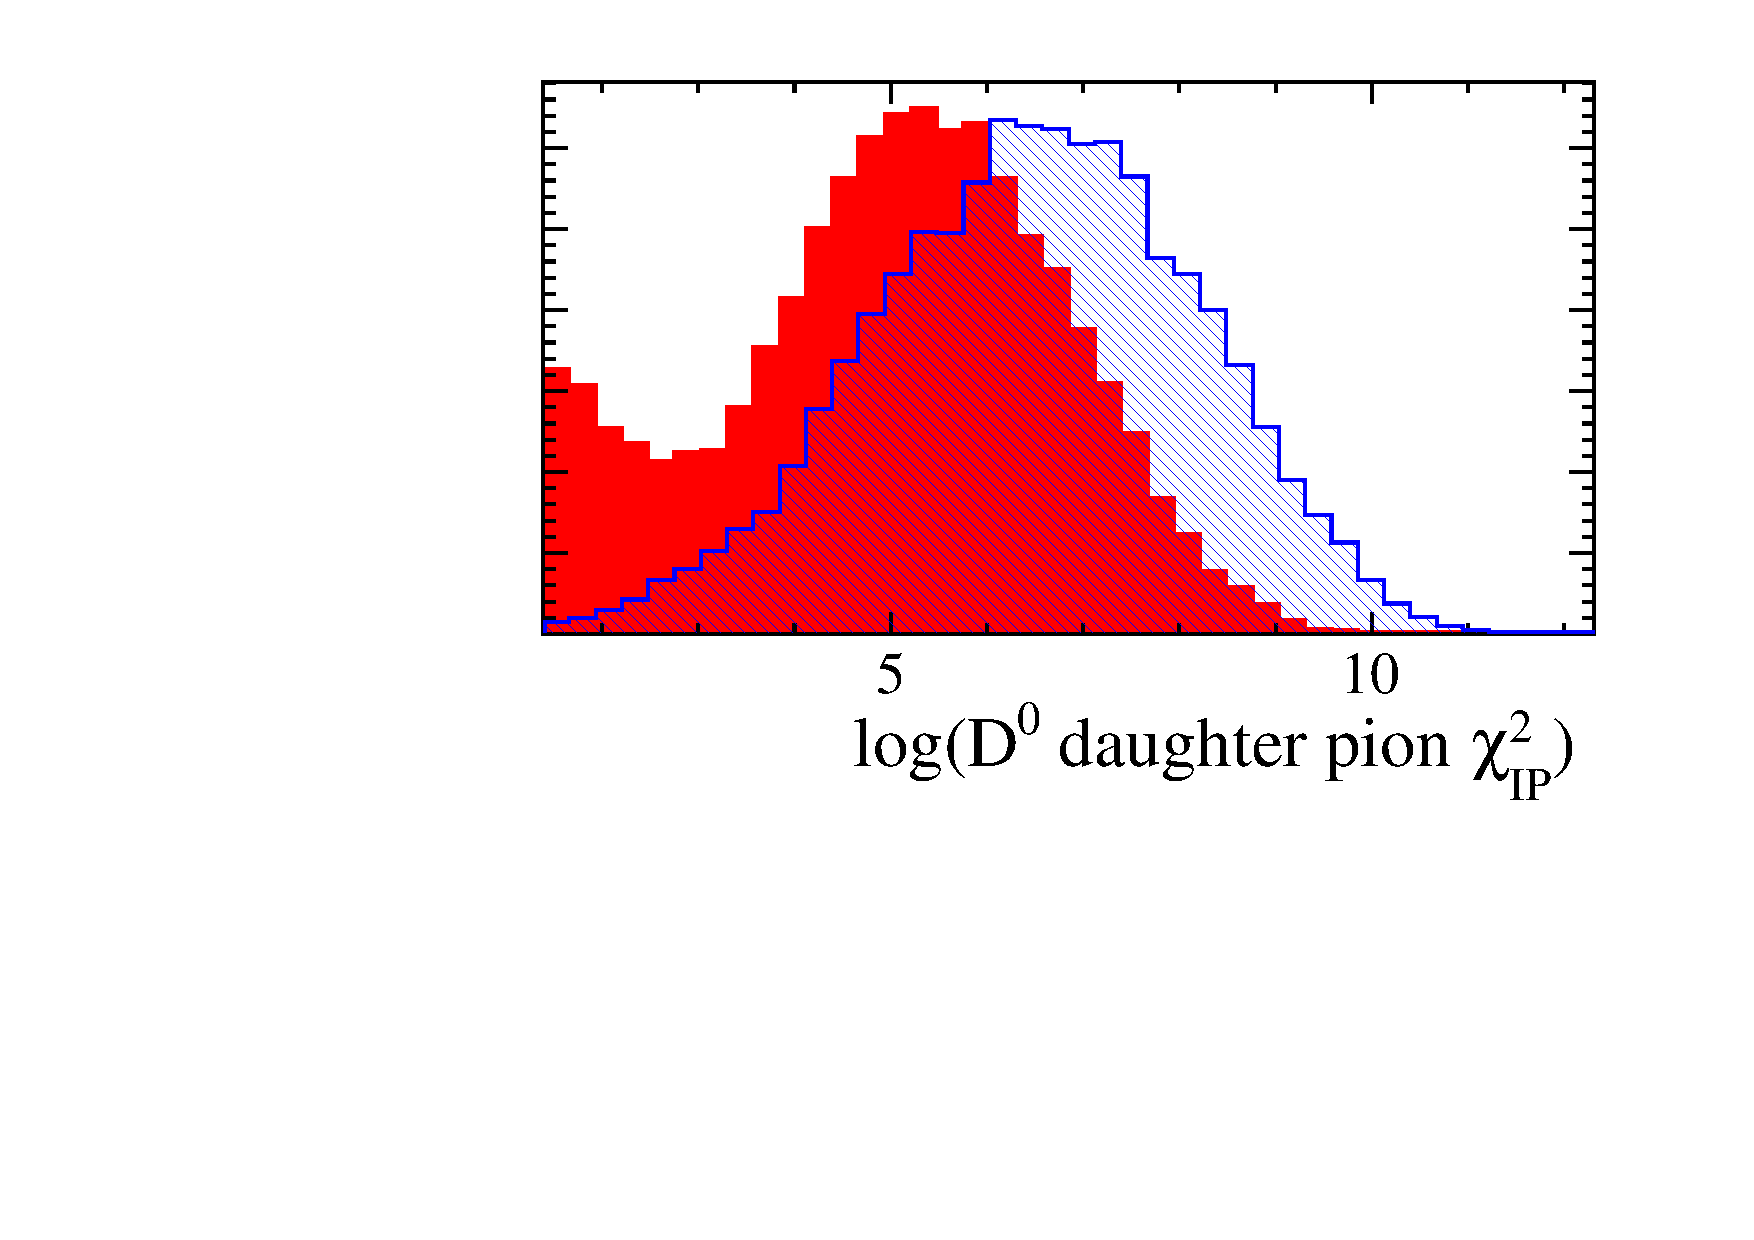
\includegraphics[width=0.3\linewidth]{figures/selection/BDTvariables/BDT_Var_KPi_DD_log_Dh2_IPCHI2_OWNPV_.pdf}
\hfill
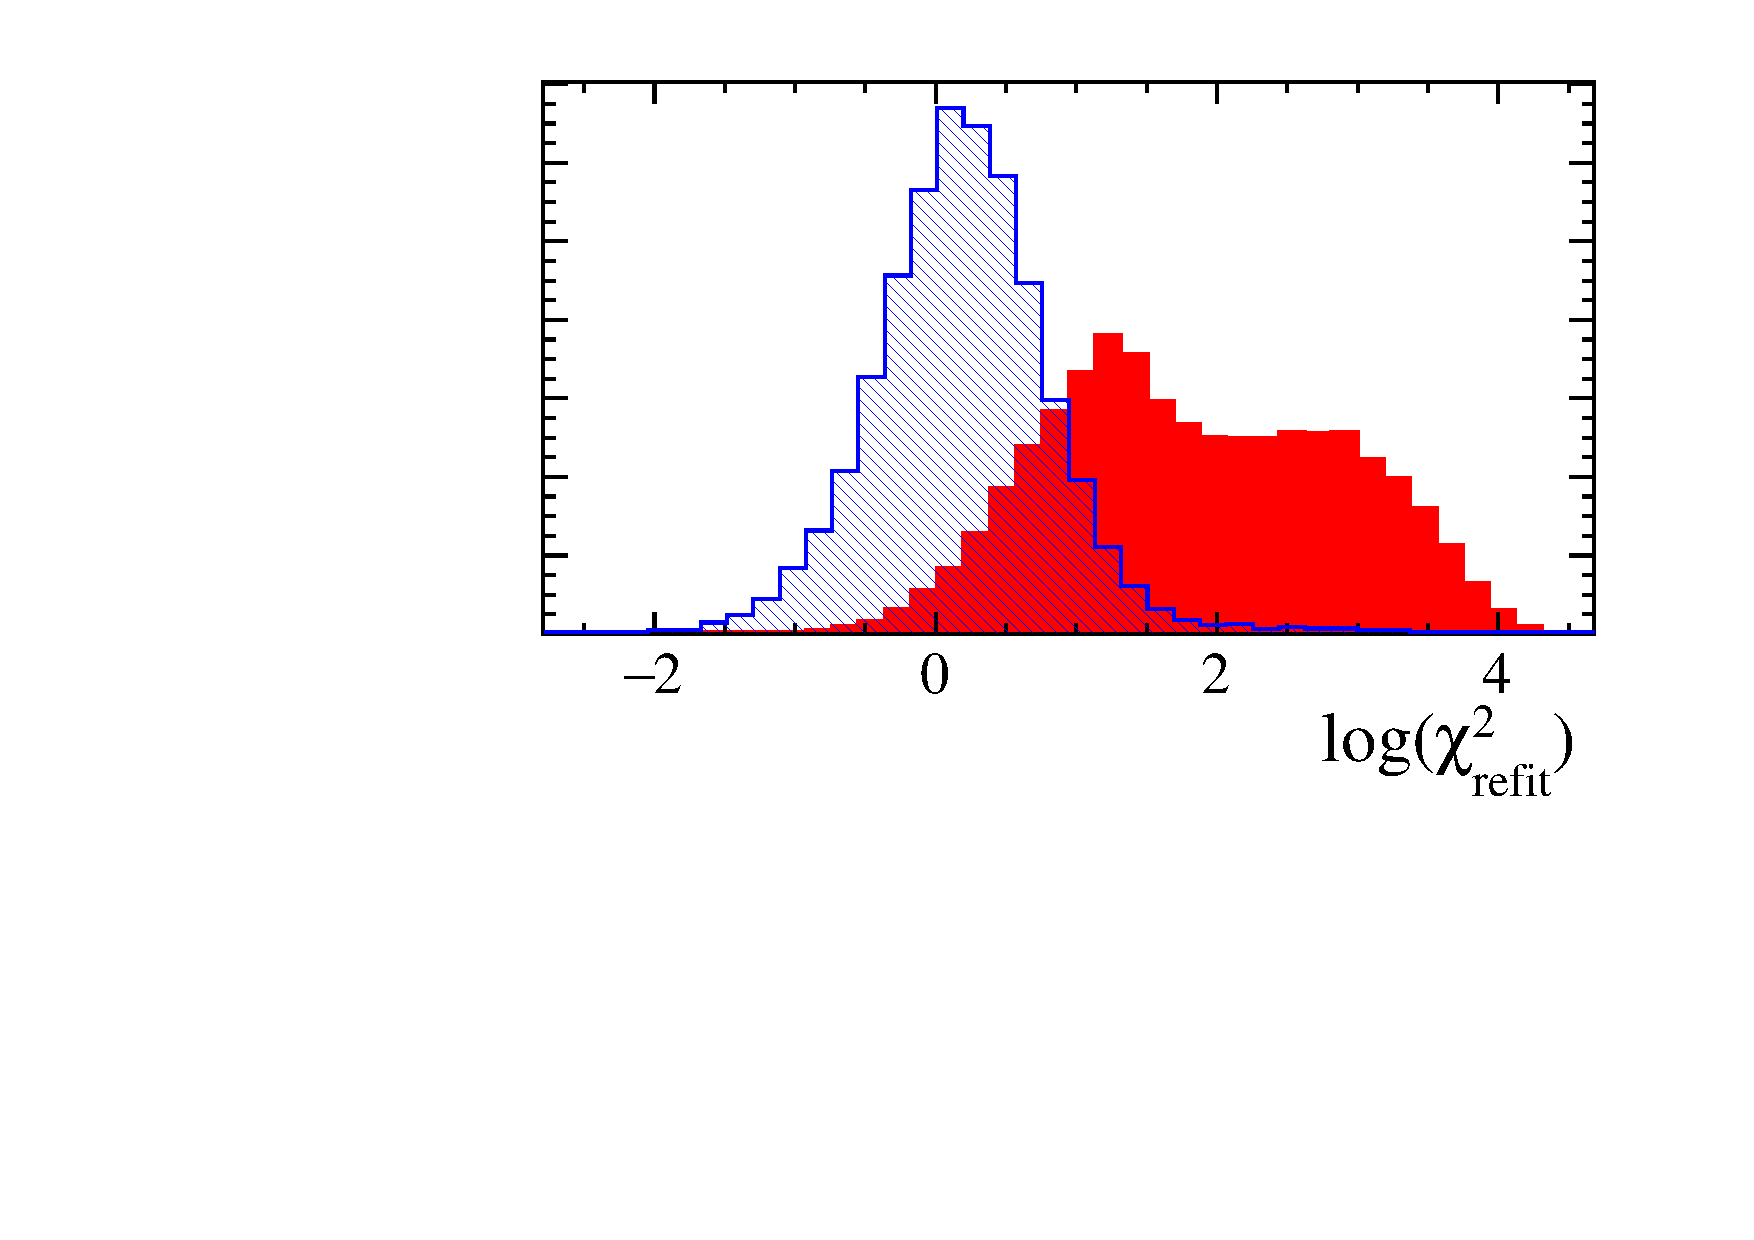
\includegraphics[width=0.3\linewidth]{figures/selection/BDTvariables/BDT_Var_KPi_DD_log_Bu_D0constKS0constPVconst_CHI2NDOF_.pdf}
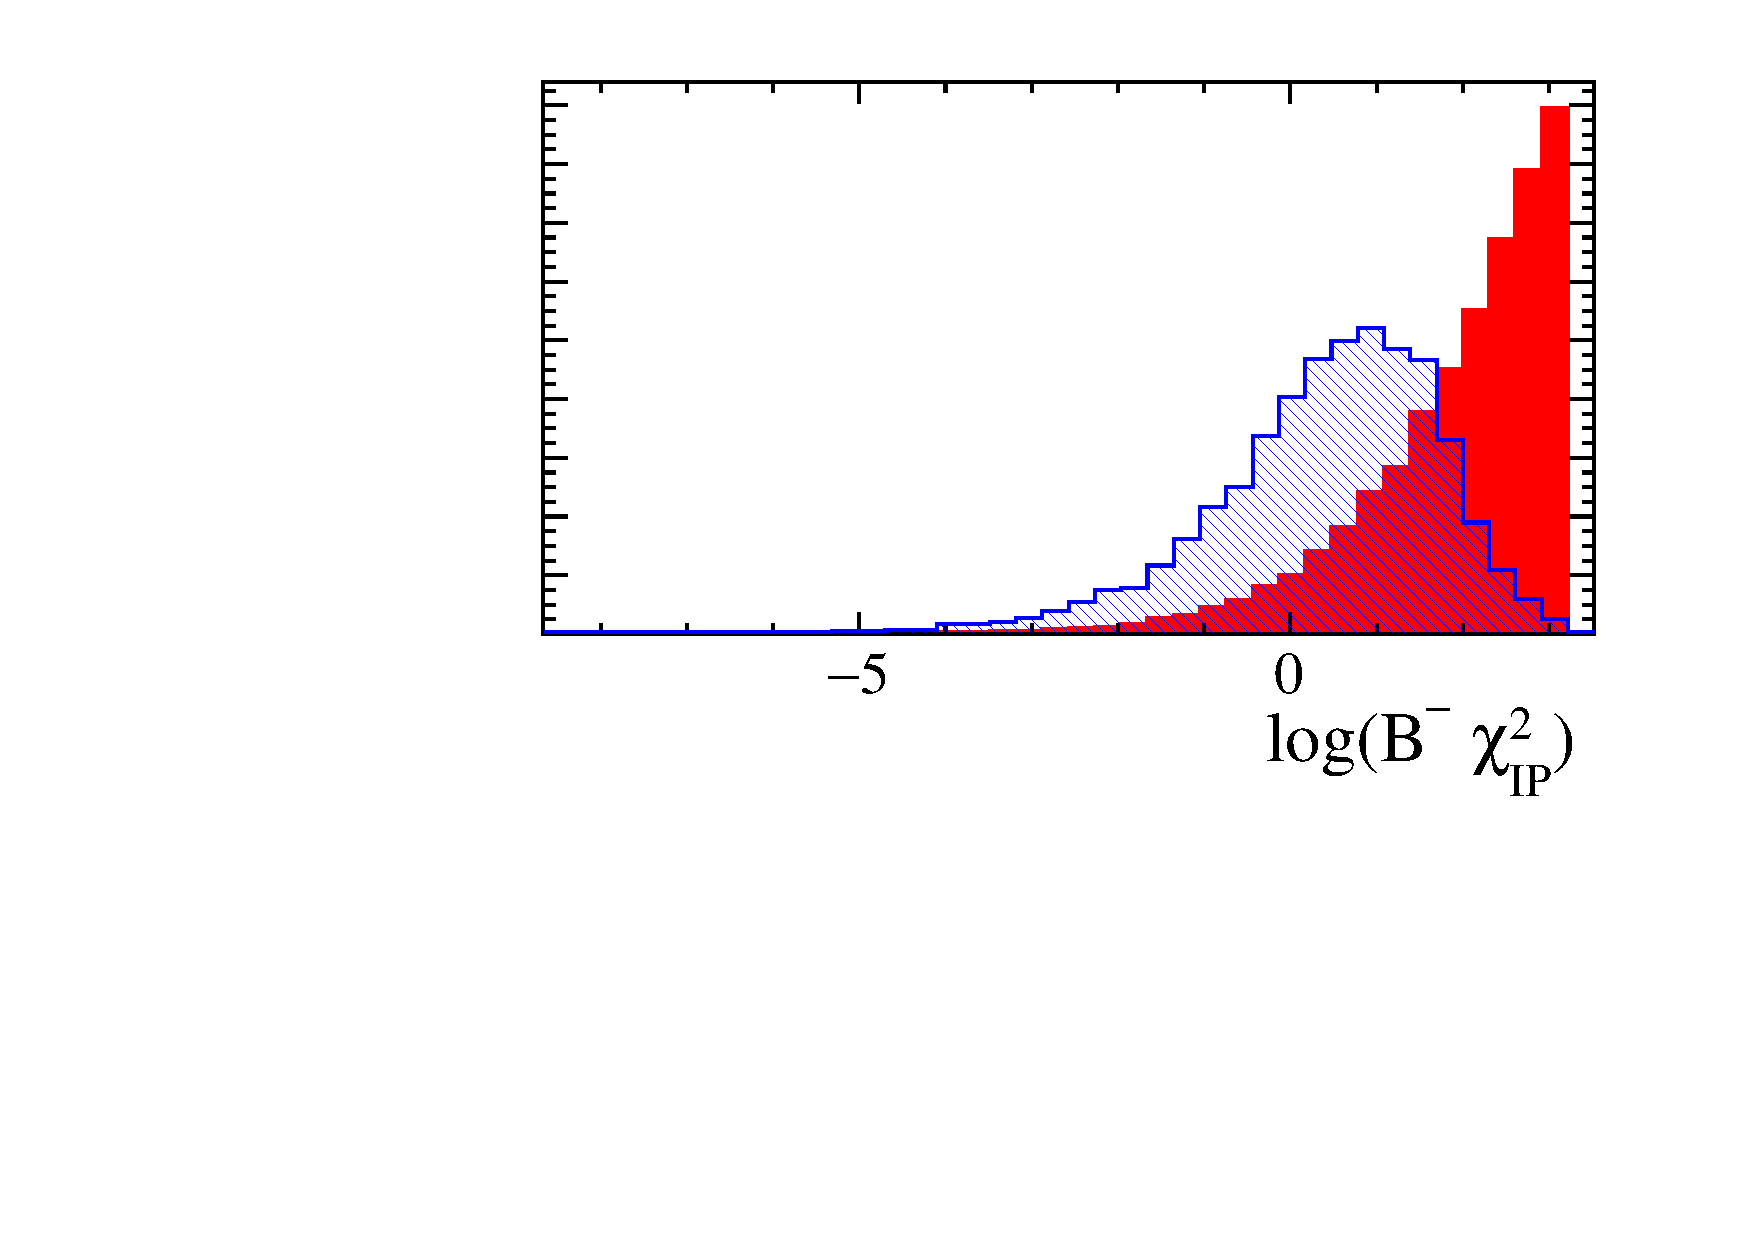
\includegraphics[width=0.3\linewidth]{figures/selection/BDTvariables/BDT_Var_KPi_DD_log_Bu_IPCHI2_OWNPV_.pdf}
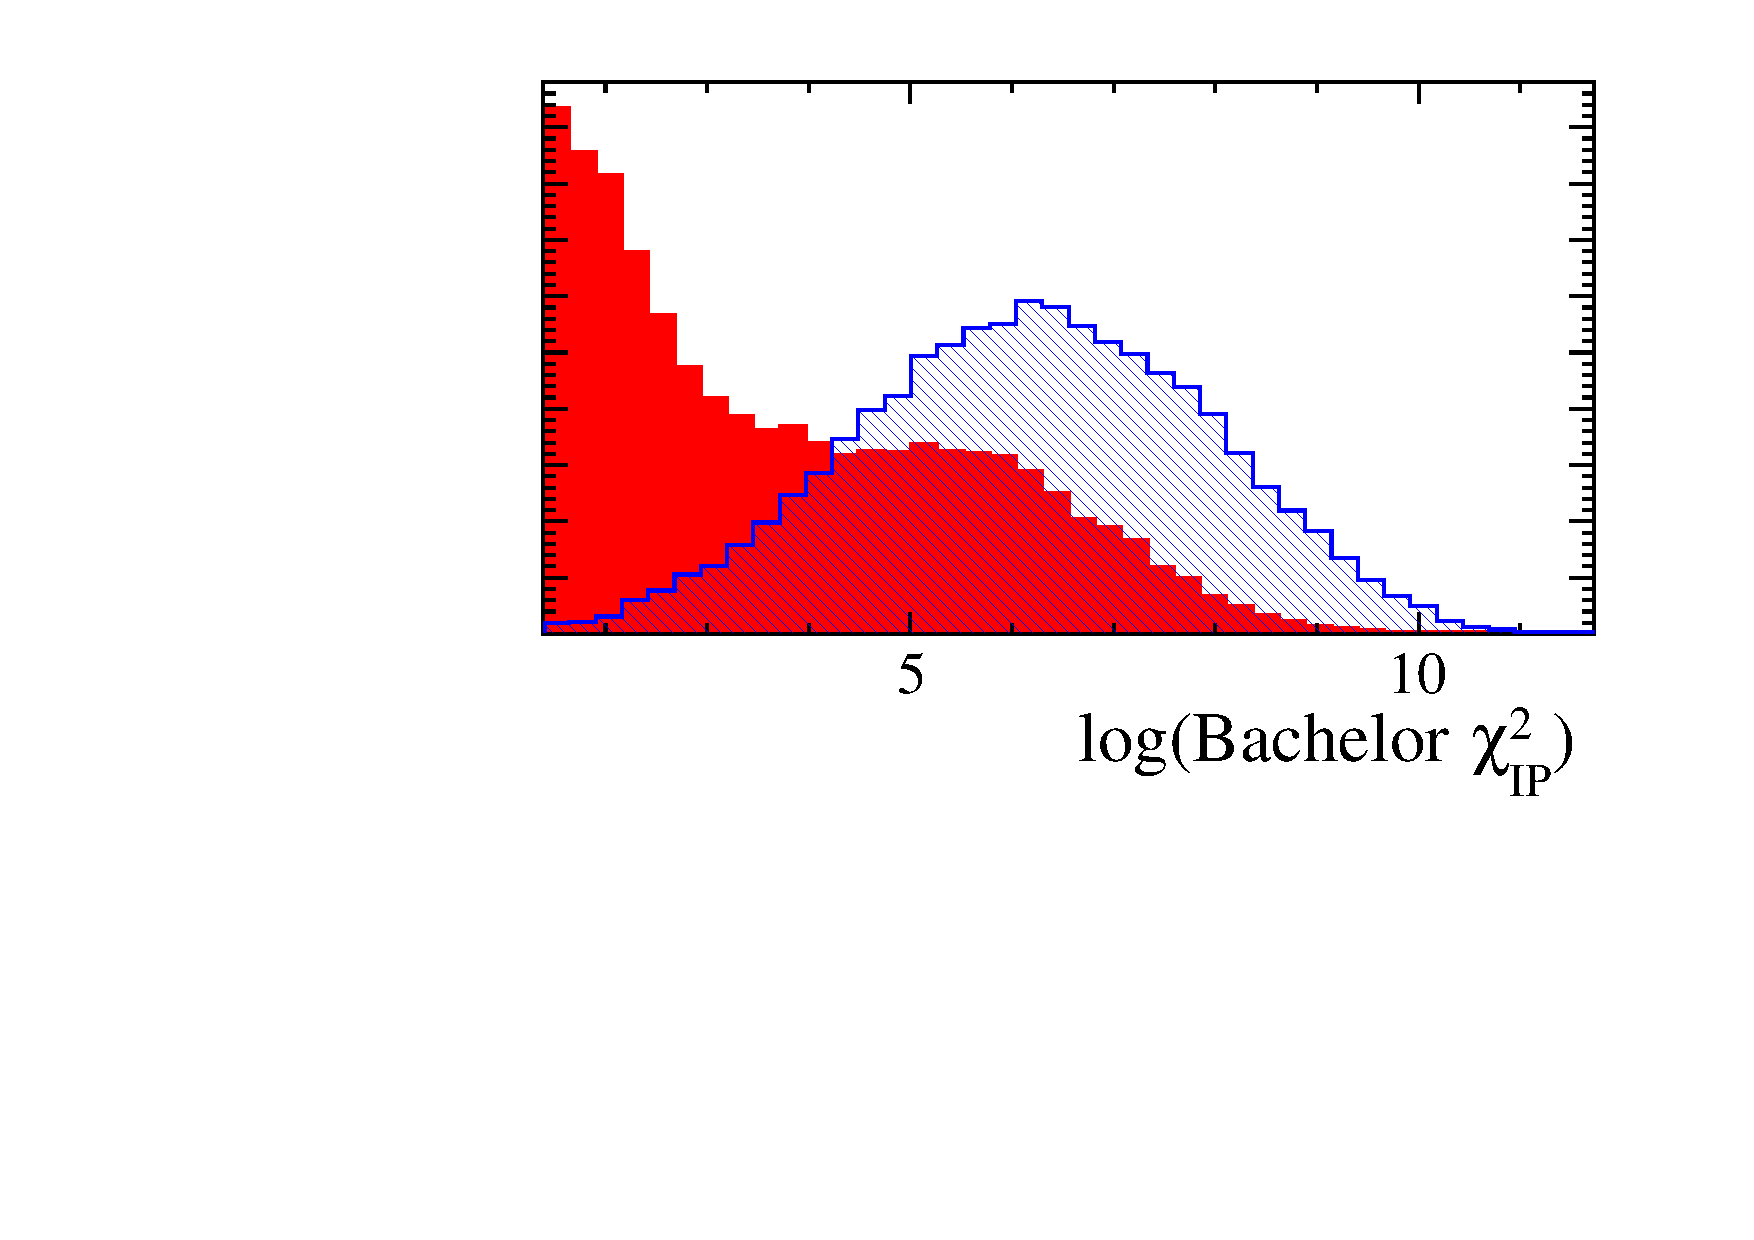
\includegraphics[width=0.3\linewidth]{figures/selection/BDTvariables/BDT_Var_KPi_DD_log_Bach_IPCHI2_OWNPV_.pdf}
\hfill
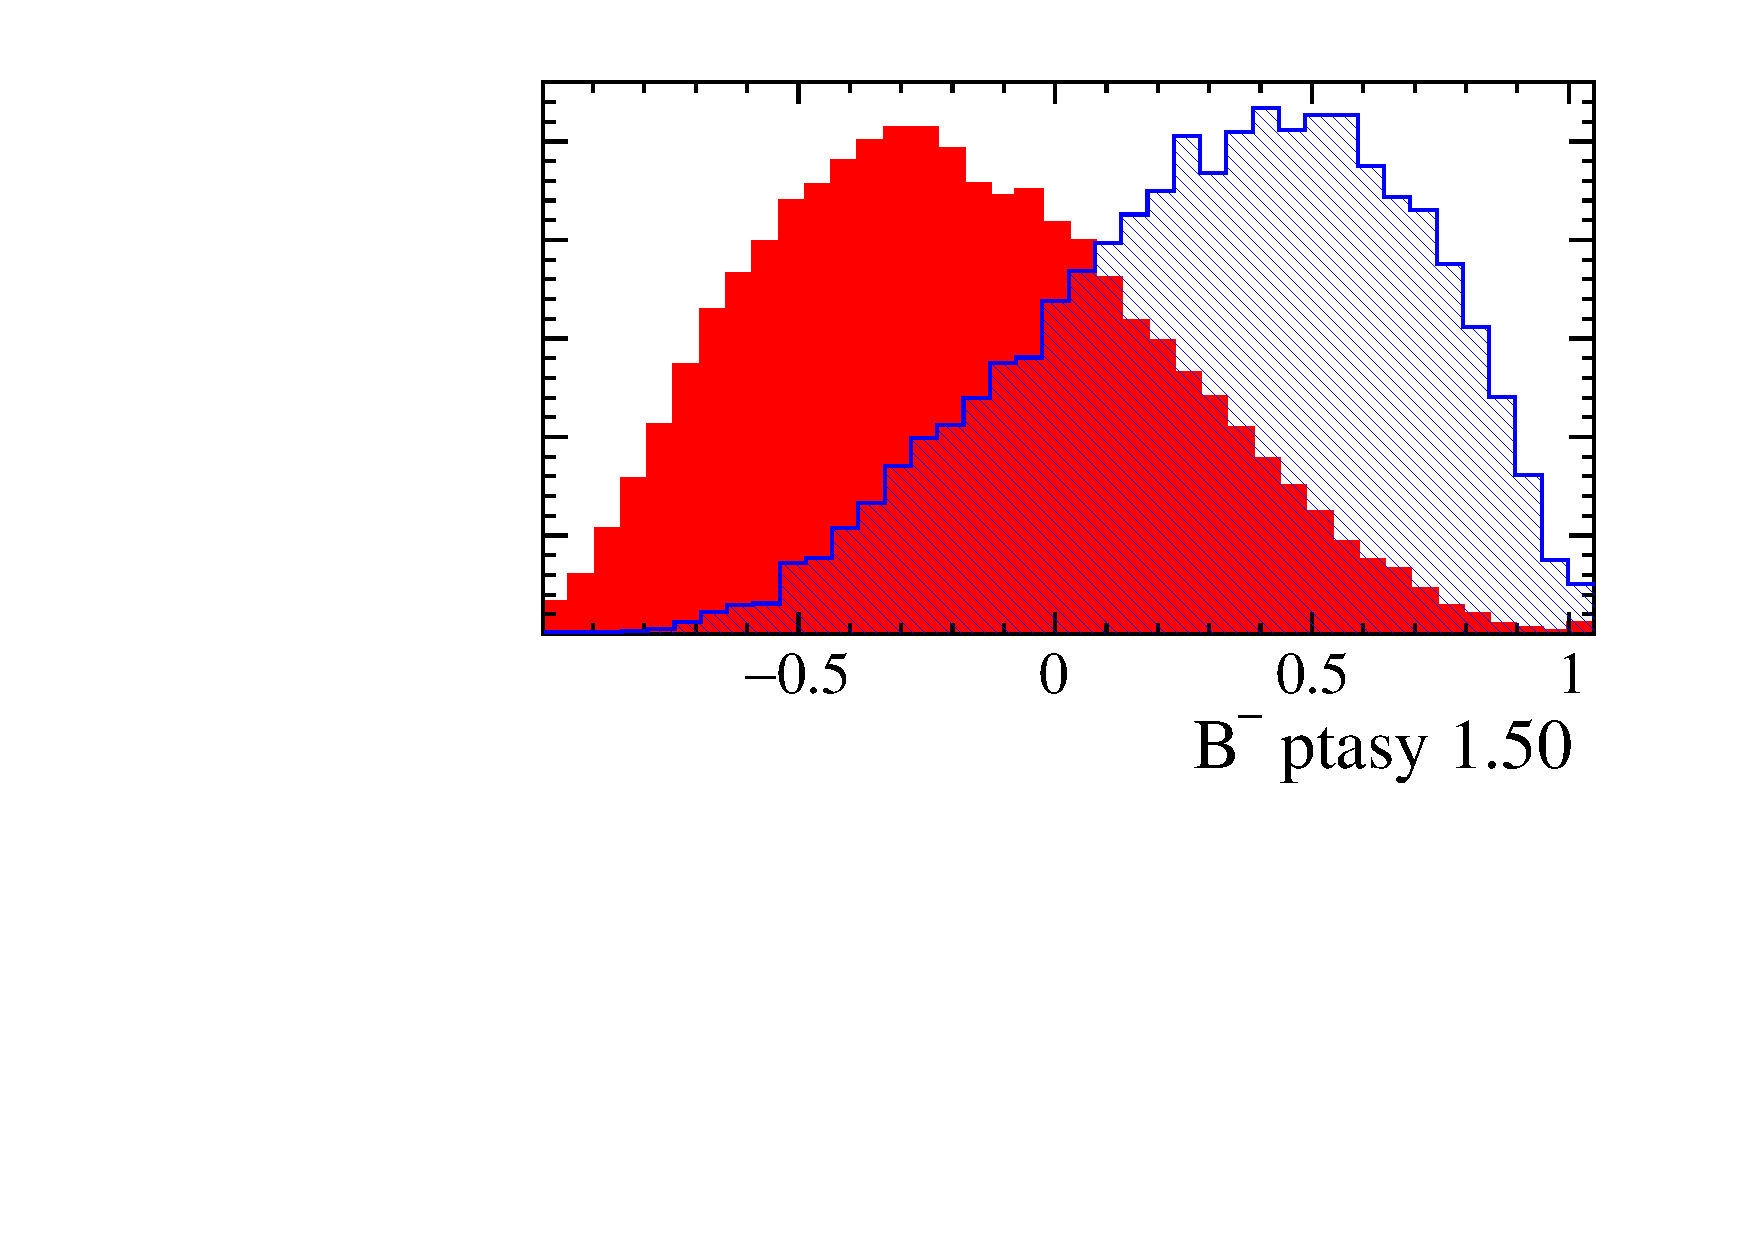
\includegraphics[width=0.3\linewidth]{{figures/selection/BDTvariables/BDT_Var_KPi_DD_Bu_ptasy_1.50}.pdf}
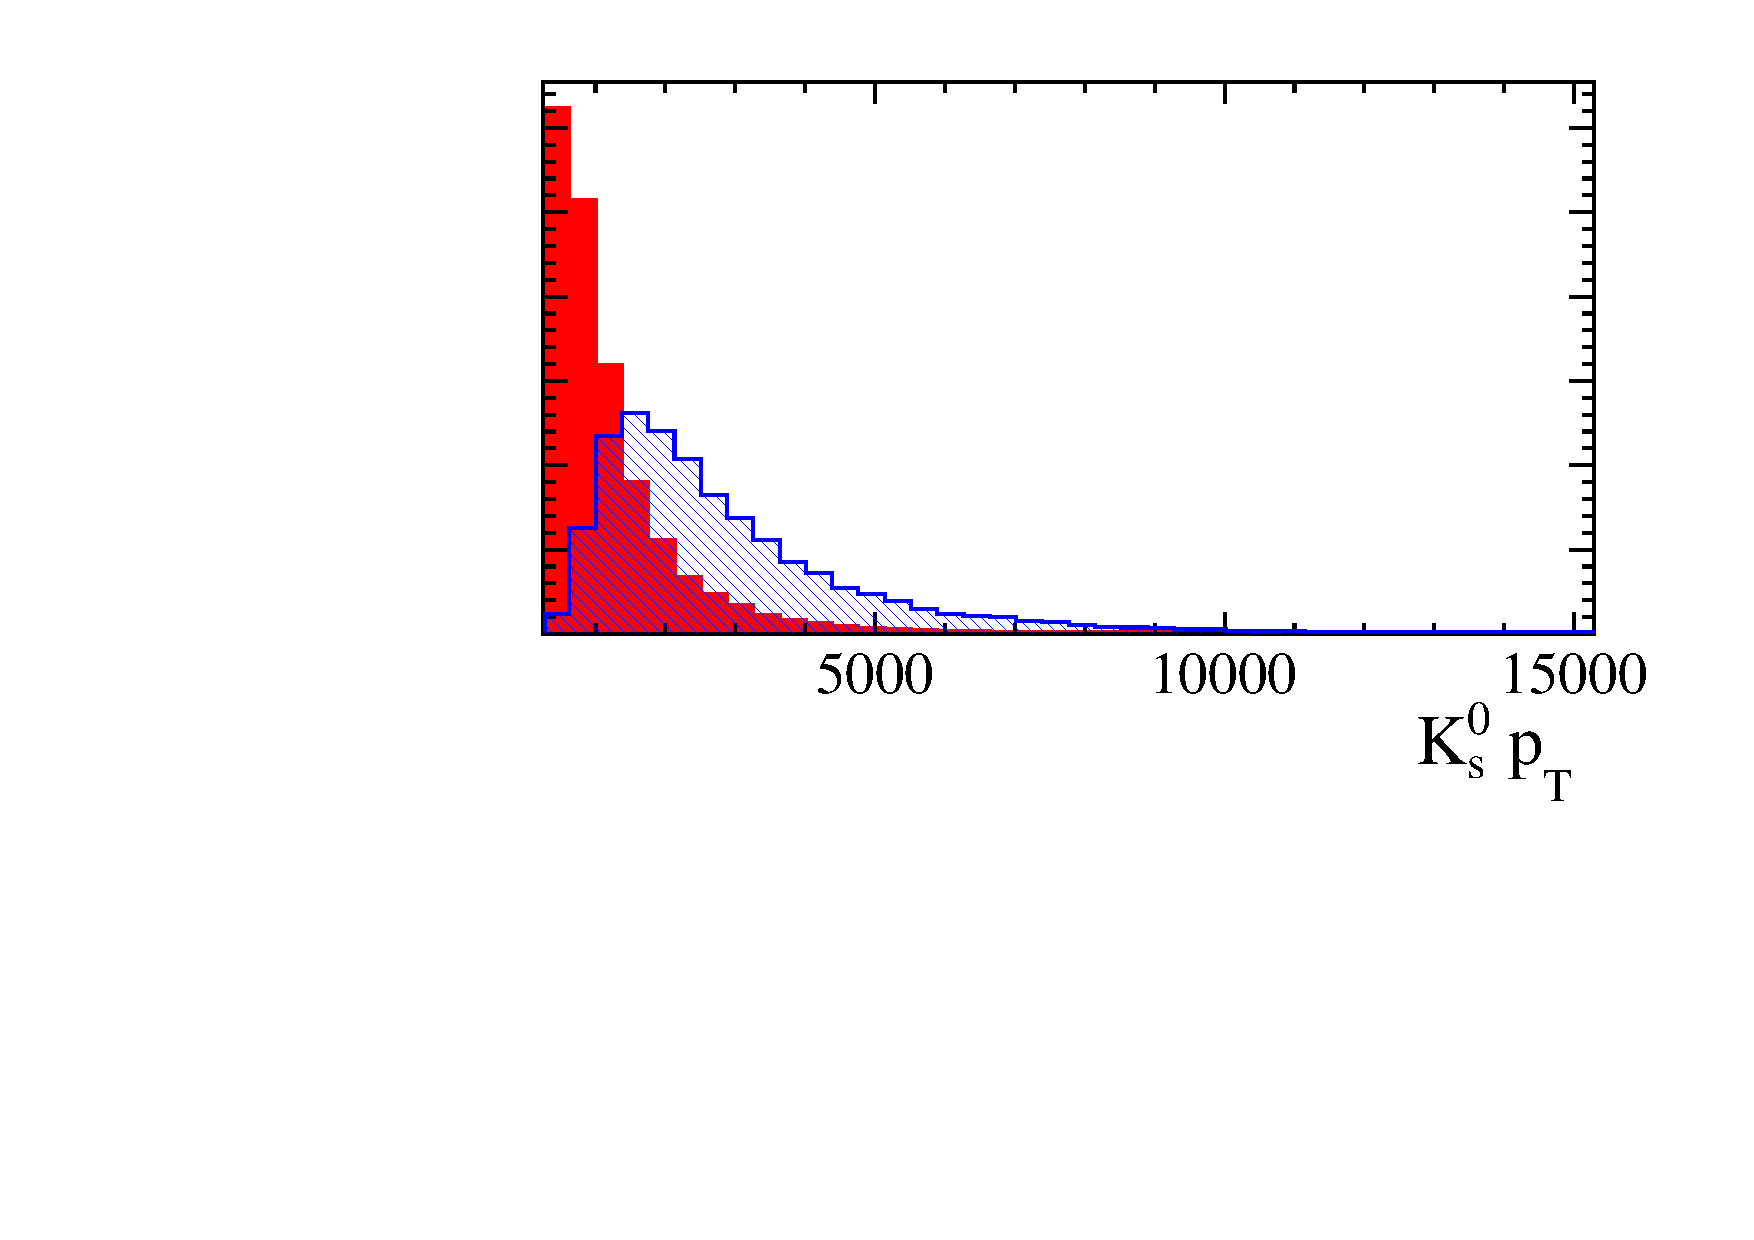
\includegraphics[width=0.3\linewidth]{figures/selection/BDTvariables/BDT_Var_KPi_DD_Ks_PT.pdf}
\caption{Distributions of the input variables using the signal (blue) and background (red) training samples for the two-body DD BDT. The variable $A_{\pt}$ represents the \pt asymmetry as defined in \eqn~\ref{ptasy}. All distributions have been normalised to unity in order to easily compare their shape, therefore the vertical axis is not labelled as it is not of interest here.}
\label{BDTinputdist2bodyDD}
\end{figure}

%\begin{figure}
%\centering
%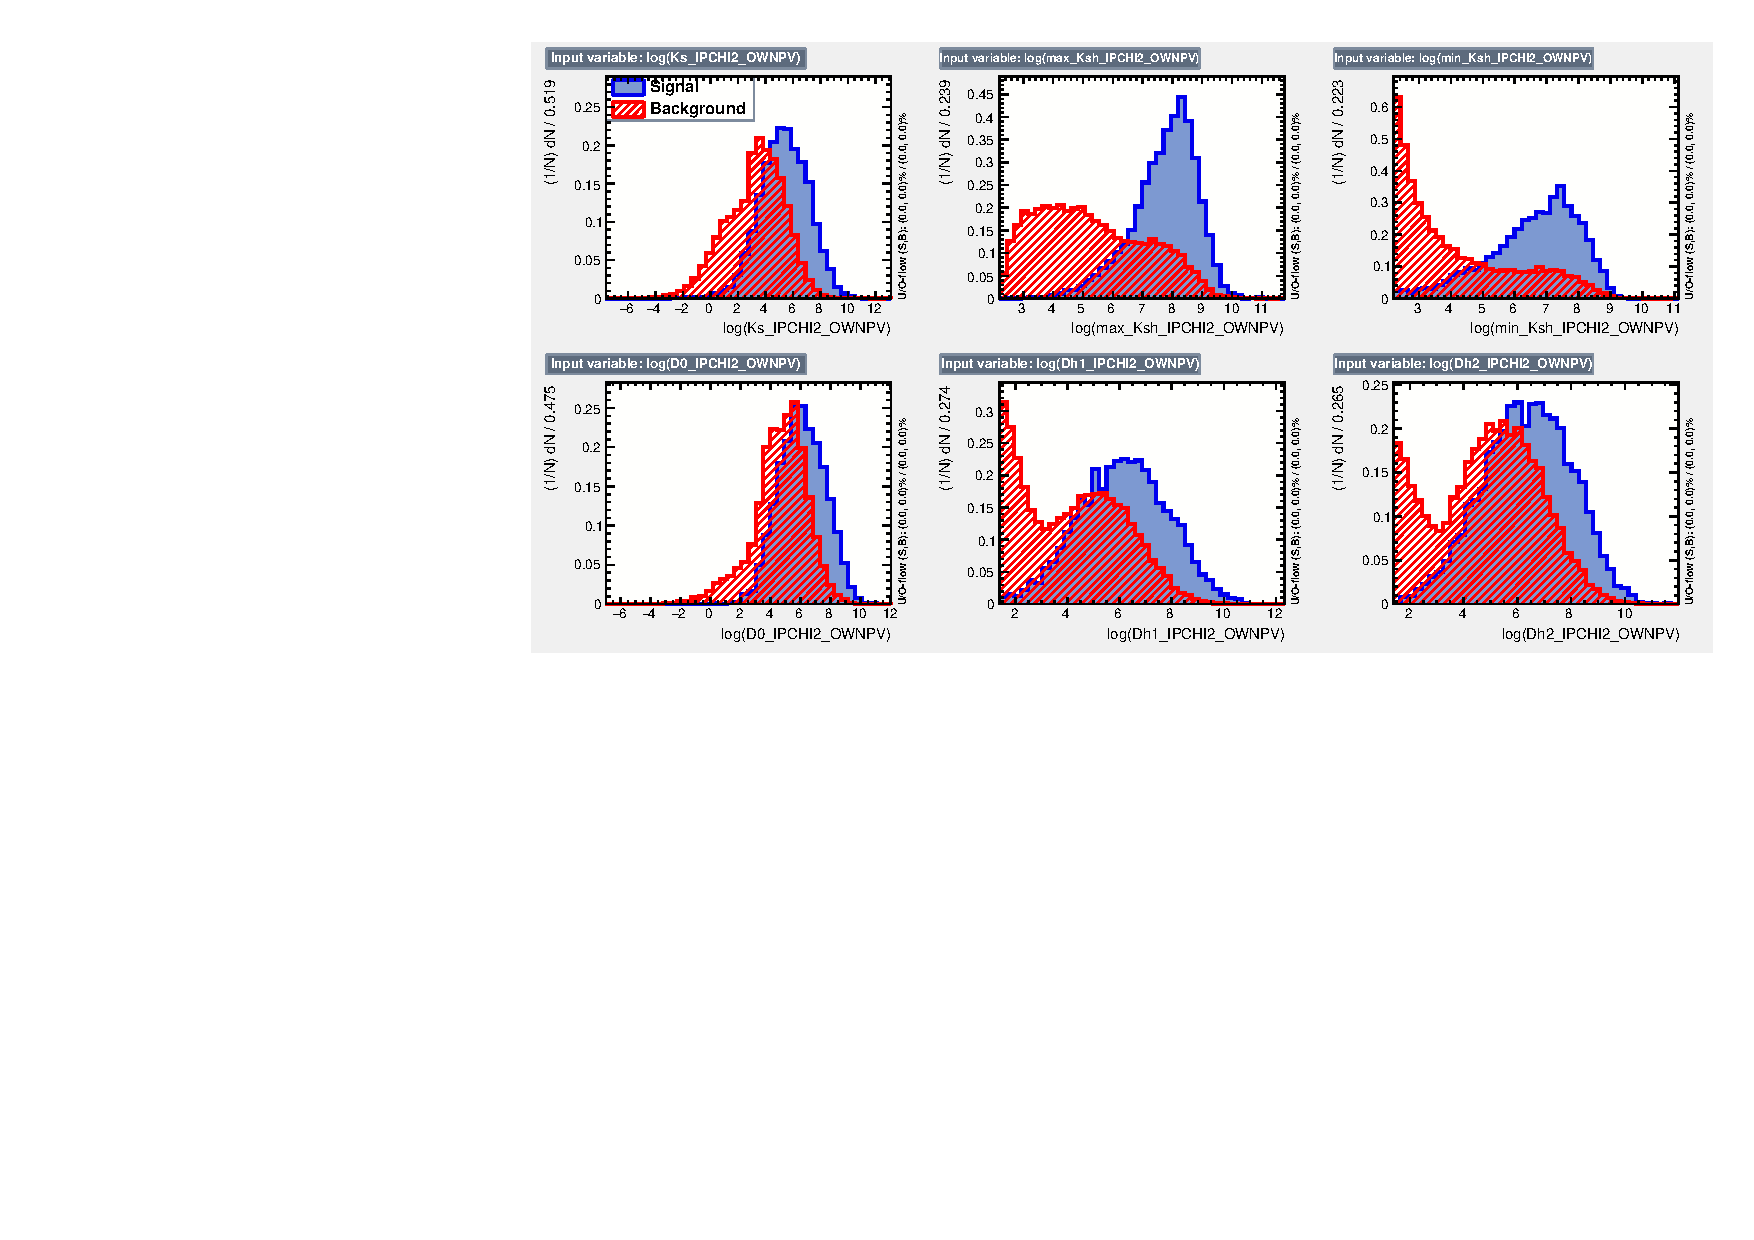
\includegraphics[width=\linewidth]{figures/selection/inputvariables_KPi_LL_run1_1.pdf}
%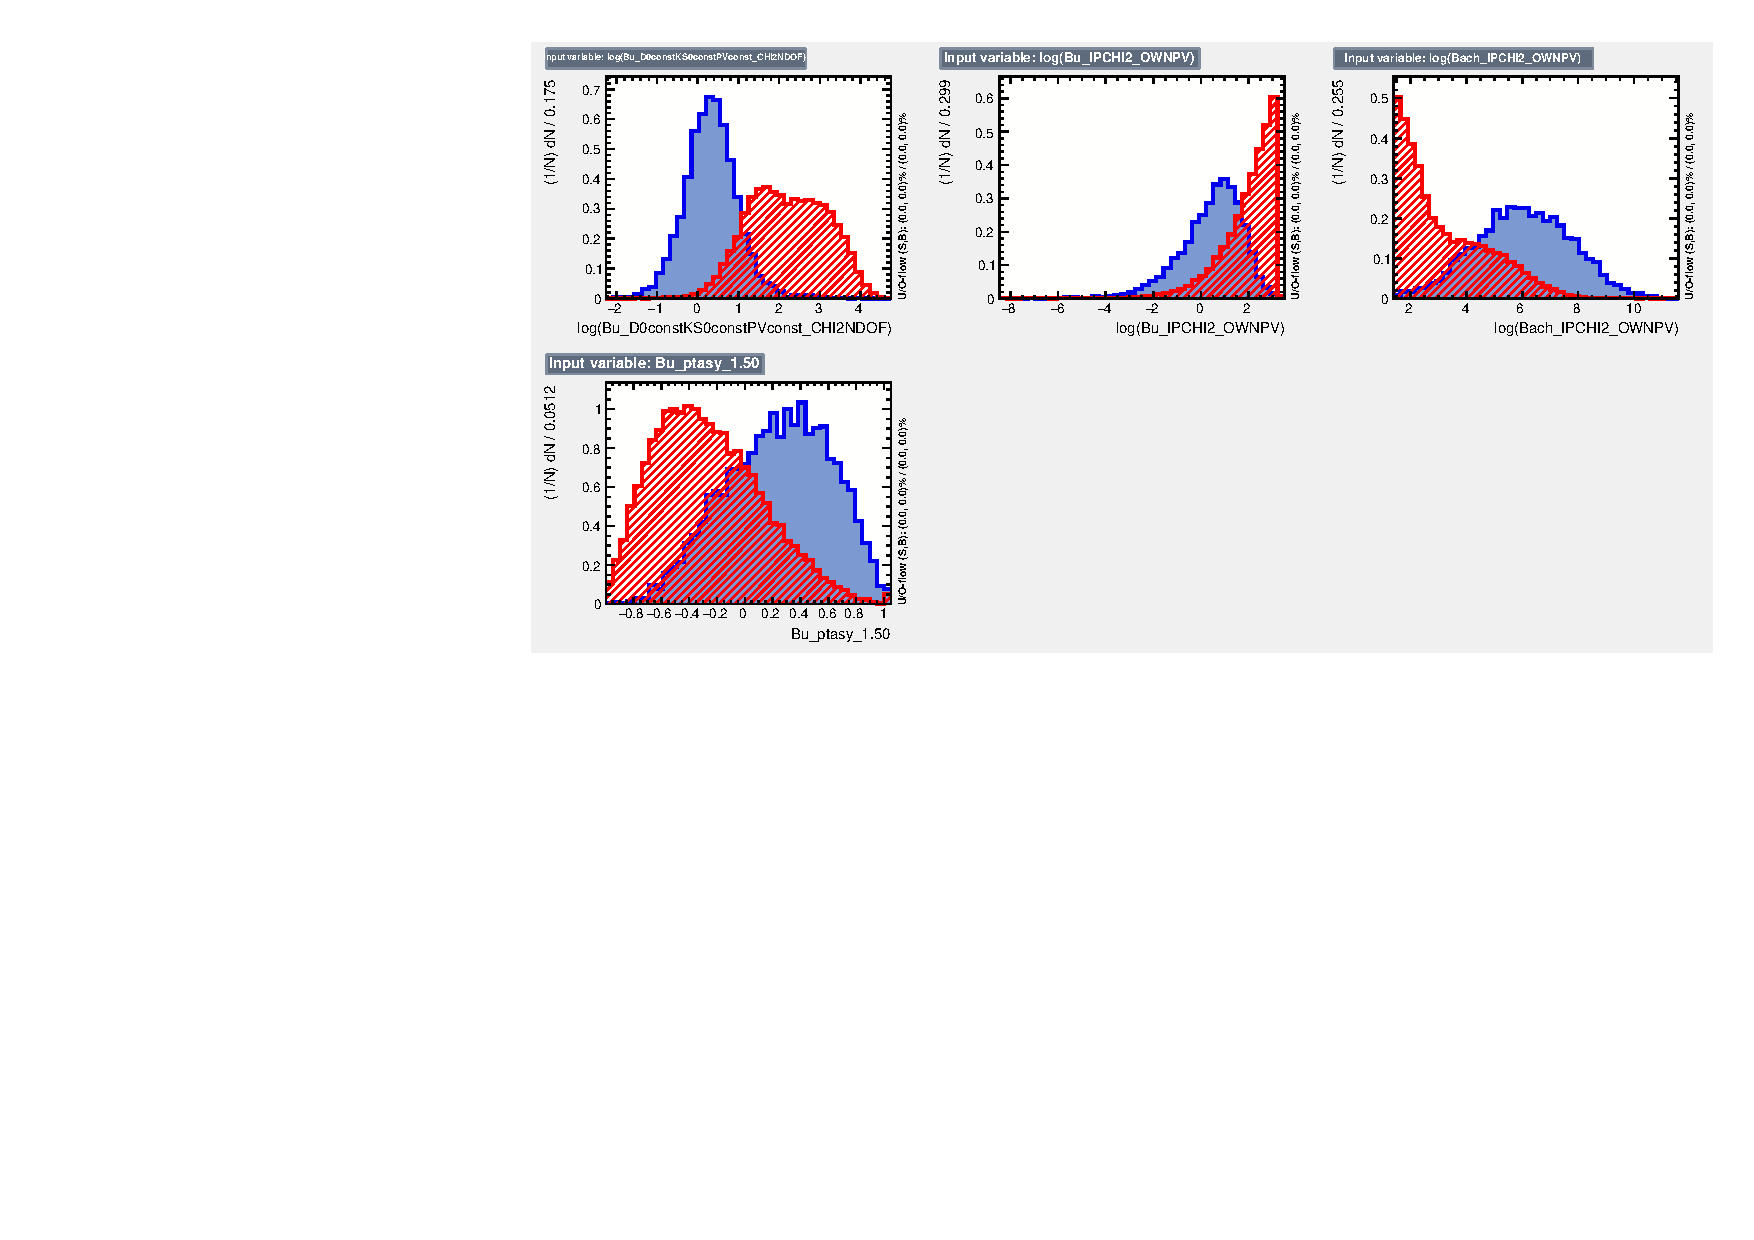
\includegraphics[width=\linewidth]{figures/selection/inputvariables_KPi_LL_run1_2.pdf}
%\caption{Distributions of the input variables using the signal (red) and background (blue) training samples for the two-body LL BDT.}
%\label{BDTinputdist2bodyLL}
%\end{figure}
%
%\begin{figure}
%\centering
%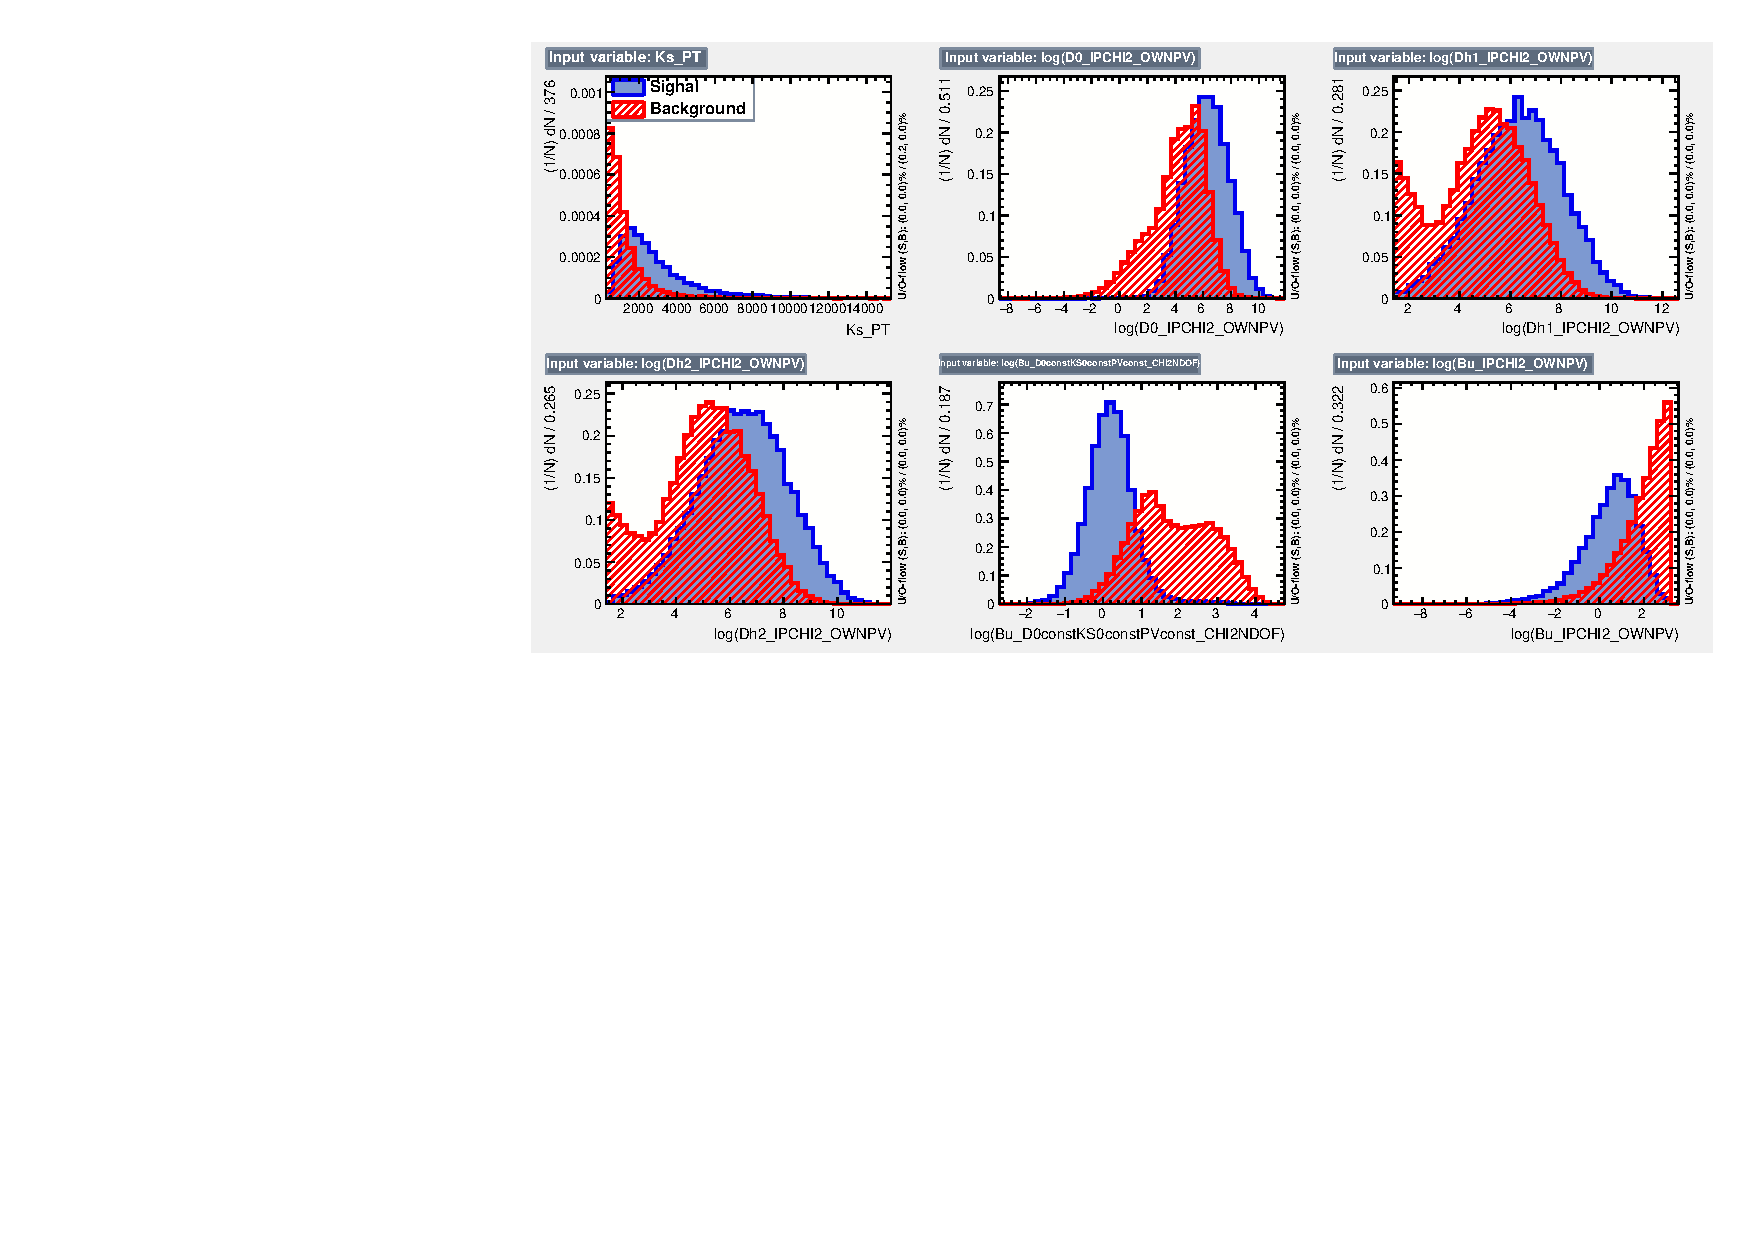
\includegraphics[width=\linewidth]{figures/selection/inputvariables_KPi_DD_run1_1.pdf}
%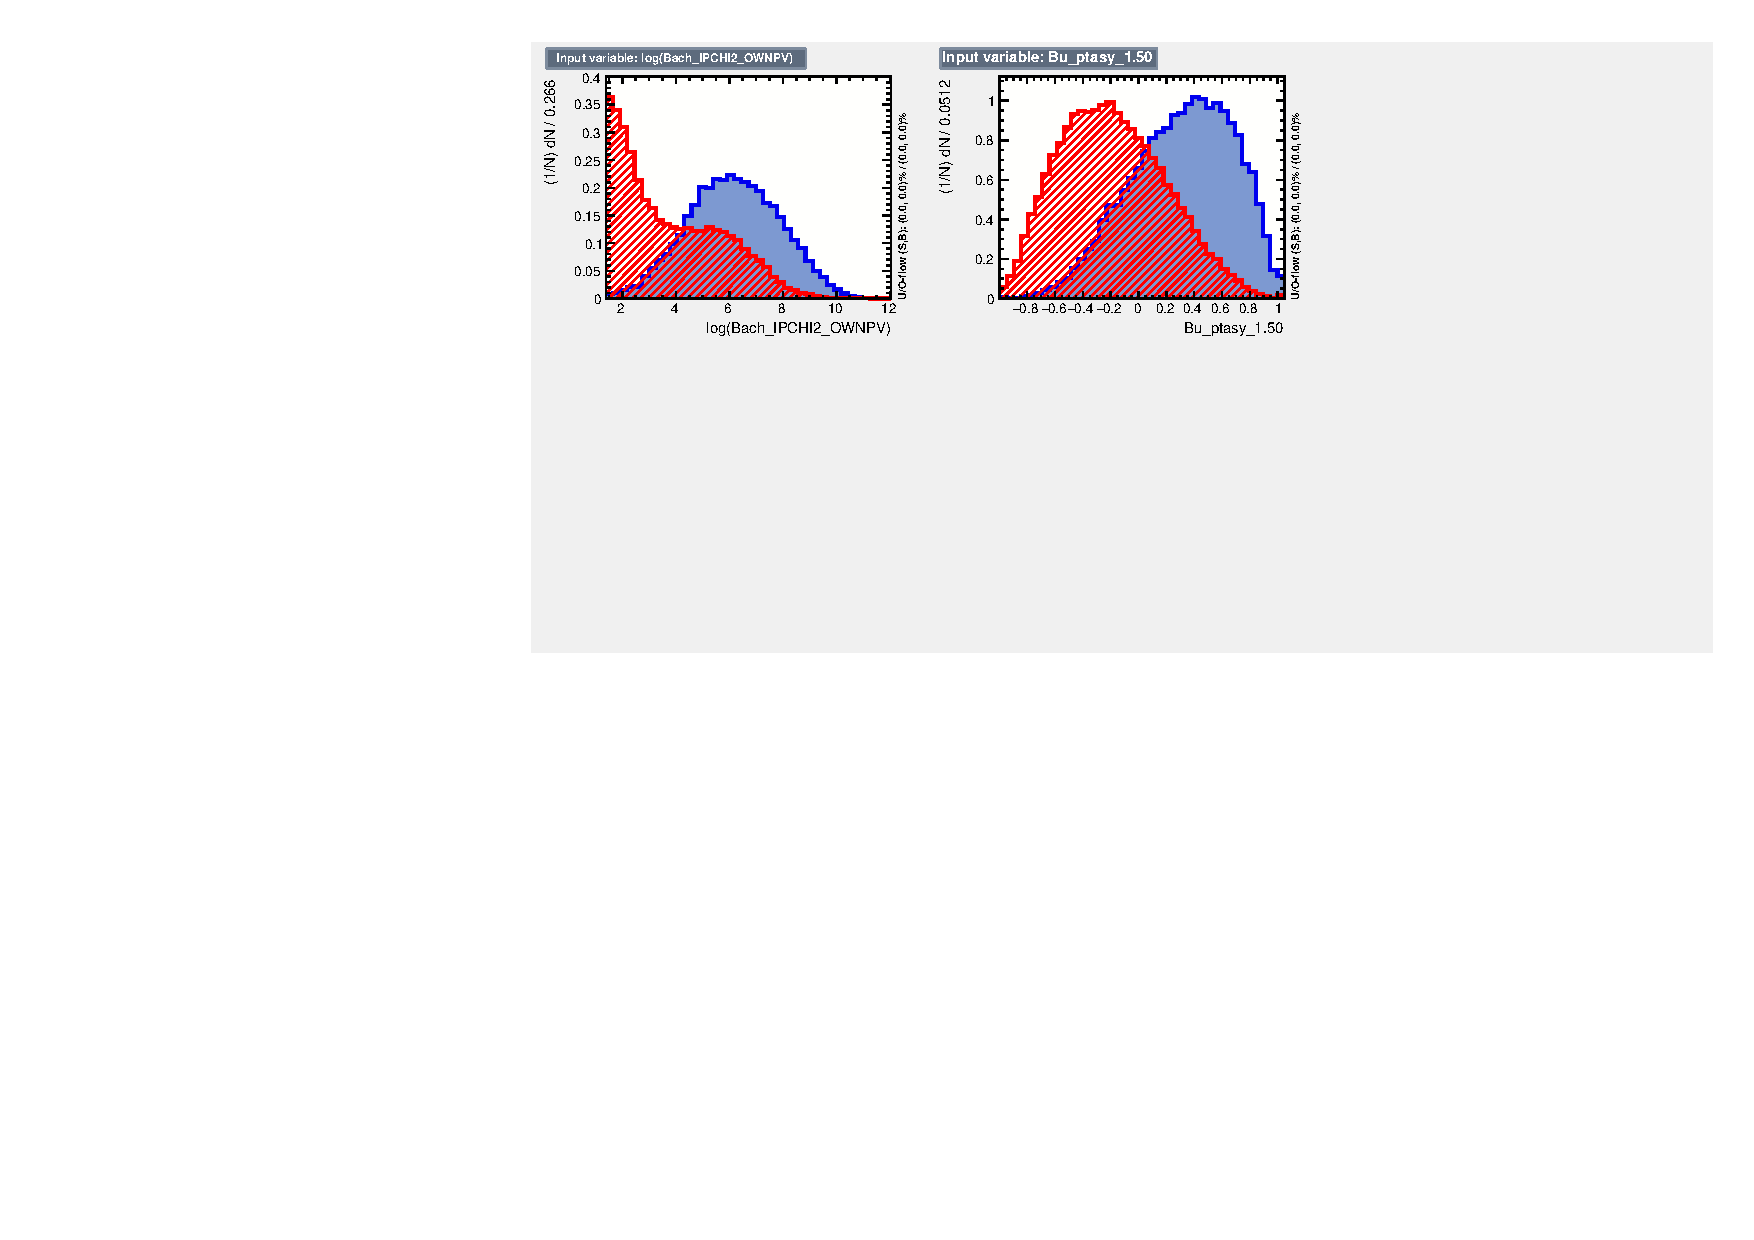
\includegraphics[trim = 0mm 50mm 0mm 0mm, clip,width=\linewidth]{figures/selection/inputvariables_KPi_DD_run1_2.pdf}
%\caption{Distributions of the input variables using the signal (red) and background (blue) training samples for the two-body DD BDT.}
%\label{BDTinputdist2bodyDD}
%\end{figure}

\subsubsection{Performance of the multivariate algorithm and choice of working point}

Selections are optimised for minimising the uncertainty in the \CP observables. This method requires the full fit and is described in \sect\ref{sec:cpfit:optimisation}. The final BDT requirements chosen, based on this optimisation, are given in \tab\ref{bdtrequirements}. The corresponding signal and background efficiencies in the two- and four-body \Dz decay modes are given in \tab\ref{BDTresults}. The performance of the two- and four-body BDT for the LL and DD categories are very similar, with signal efficiency above 90\% and background efficiency of less than 6\%. 

\begin{table}
\centering
\begin{tabular}{c|cc}
 & LL & DD \\
\hline
All \Dz modes except the ADS modes & 0.6 & 0.7 \\
ADS modes & 0.6 & 0.9 \\
\end{tabular}
\caption{BDT requirements for each of the \Dz decay modes, where the BDT classifier must be greater than the values in the table, for both LL and DD candidates.}
\label{bdtrequirements}
\end{table}

\begin{table}
\centering
\begin{tabular}{c|cc}
& LL & DD \\
\hline
\kpi & 0.95 (0.06) & 0.90 (0.05) \\
\kpipipi & 0.95 (0.04) & 0.93 (0.03) \\
\end{tabular}
\caption{Signal (background) efficiencies averaged across the whole dataset for the chosen BDT requirements in both \kpi and \kpipipi modes.}
\label{BDTresults}
\end{table}


\subsection{Summary of the selection requirements}
\label{sec:selection:summary}

\Tab\ref{selectionsummary} lists a summary of the selection requirements applied to both two- and four-body \btodkst decays to combinatorial background events and peaking backgrounds. 

\begin{table}[h]
\centering
\resizebox{\textwidth}{!}{
\begin{tabular}{c|c}
\hline
\textbf{Variable} & \textbf{Selection requirement} \\
\hline \hline
\multicolumn{1}{l}{\textbf{Mass variables}} & \\
\hline \hline
$\textbar$ \Dz mass - 1864.86~\mevcc $\textbar$ & $<$ 25~\mevcc \\
$\textbar$ \KS mass - 497.614~\mevcc $\textbar$ & $<$ 15~\mevcc for LL, $<$ 20~\mevcc for DD \\
$\textbar$ \Kstarm mass - 892~\mevcc $\textbar$ & $<$ 75~\mevcc \\
\hline \hline
\multicolumn{1}{l}{\textbf{PID and veto}} & \\
\hline \hline
DLLK of bachelor & $<$ 4 \\
DLLK of D daughters (two-body) & $>$ 2 for all kaons, $<$ -2 for all pions \\
DLLK of D daughters (\decay{\Dz}{\Km\pip\pim\pip}) & $>$ 2 for \Km, $<$ -2 for both \pip mesons \\
DLLK of D daughters (\decay{\Dz}{\pim\pip\pim\pip}) & $<$ -2 for both \pip mesons \\
$\textbar \Dz_{swapped} - 1864.86 \mevcc \textbar$ for ADS modes & $>$ 15 \mevcc \\
\hline \hline
\multicolumn{1}{l}{\textbf{Other backgrounds}} & \\
\hline \hline
$\textbar \cos(\theta_{\KS}) \textbar$ & $>$ 0.3 \\
\Dz FD significance & $>$ 2 \\
\KS FD significance & $>$ 5 for LL, no requirement for DD \\
\Bm \chisqip & 0 - 25 \\
\Bm \chisq/dof & 0 - 100 \\
\hline \hline
\multicolumn{1}{l}{\textbf{BDT}} & \\
\hline \hline
BDT classifier for CF and GLW modes & $>$ 0.6 for LL, $>$ 0.7 for DD \\
BDT classifier for ADS modes & $>$ 0.6 for LL, $>$ 0.9 for DD \\
\hline
\end{tabular}}
\caption{Summary of the selection requirements applied to two- and four-body \btodkst decays in this analysis.}
\label{selectionsummary}
\end{table}

\subsection{Final refitted \Bm mass distributions}

The reconstructed \Bm mass distributions, with constraints applied, for each of the samples passing the full selection requirements, detailed in this chapter, are given in \fig\ref{fig:finalBmass}.

\begin{figure}[h]
\centering
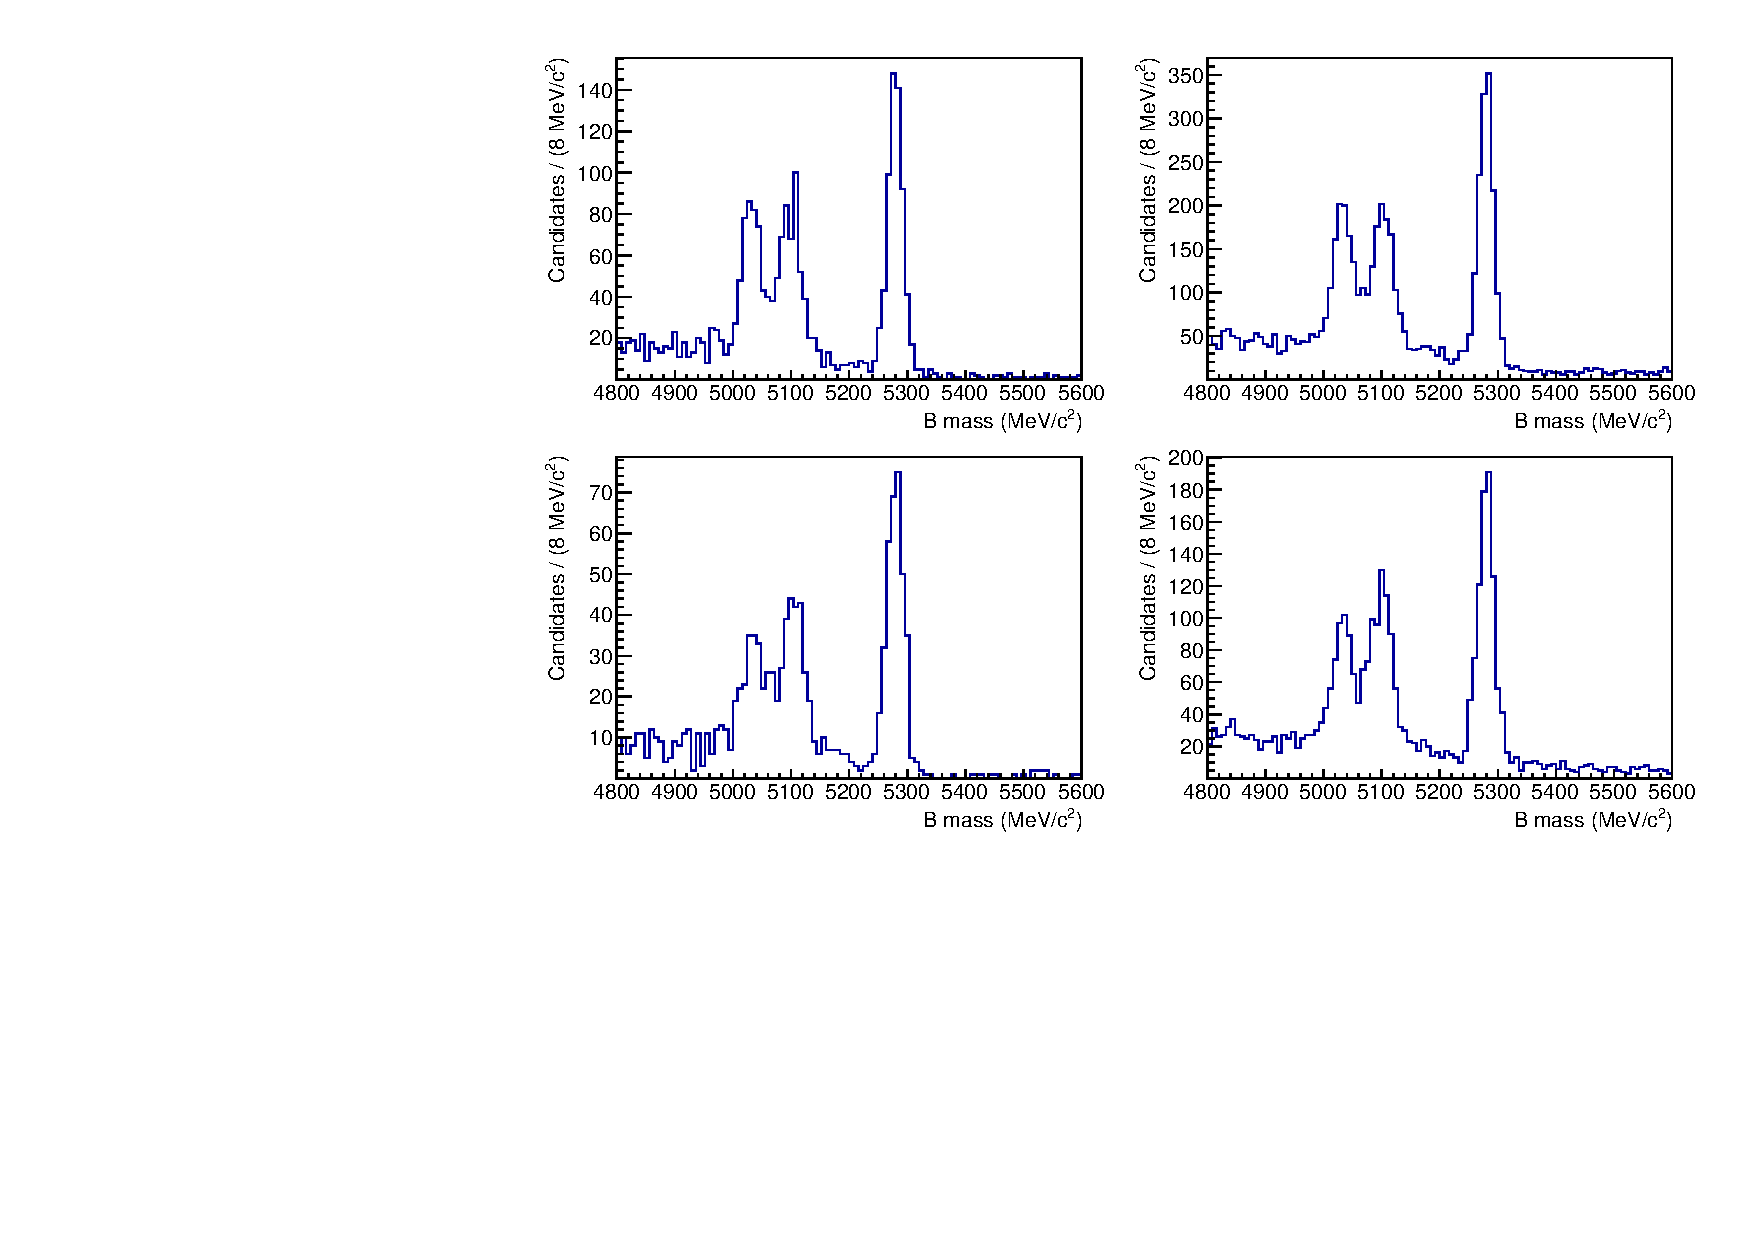
\includegraphics[width=0.8\linewidth]{figures/selection/finalBmass.pdf}
\put(-300,190) {(a)}
\put(-130,190) {(b)}
\put(-300,80) {(c)}
\put(-130,80) {(d)}
\caption{Refitted \Bm mass distributions after the full selection has been applied for (a) \kpi LL, (b) \kpi DD, (c) \kpipipi LL, and (d) \kpipipi DD candidates, with \runone and \runtwo samples combined.}
\label{fig:finalBmass}
\end{figure}

\clearpage

\section{Mass parameterisation of the favoured modes}
\label{sec:massfit}

This section describes the \Bm mass parameterisation developed for the two- and four-body favoured \Dz modes. The aim is to first develop a model that parameterises the invariant \Bm mass, and then perform fits to the \kpi and \kpipipi data from which various parameters can be extracted. This model is later applied to the suppressed \Dz decay modes when performing the simultaneous fit to measure the \CP observables, as described in Chapter~\ref{ch:5-cpfit}. There are three components considered in the model:
\begin{enumerate}
\item Signal, \decay{\Bm}{\D\Kstarm} decays,
\item Combinatorial background,
\item Partially reconstructed background.
\end{enumerate}
As some differences are found, data samples are split into the following categories: LL and DD \KS reconstruction types, \runone and \runtwo data-taking periods and two-body and four-body modes. 

\subsection{Maximum and extended maximum likelihood}
\label{sec:massfit:likelihood}

The maximum likelihood, or extended maximum likelihood, technique is used to find the best model parameters to describe the data~\cite{MLandEML,EML}. A model consists of a probability density function (PDF), $f(x;\theta)$, which is a function of a continuous random variable, $x$, and depends on various parameters, $\theta$, that control the shape of the distribution. The integral across an interval gives the probability that the value is within that interval, therefore the PDF is normalised to unity. An experiment performs $n$ independent observations of $x$, $\{x_1, x_2, ..., x_n\}$. The likelihood is the probability, for given values of the parameters, of observing a particular dataset,
\begin{equation}
L(\theta;x) = \prod_{i=1}^{n} f(x_i;\theta).
\end{equation}
The parameters are extracted for a given dataset by finding the best combination of these parameters that maximise the likelihood~\cite{MLandEML}. The maximum likelihood technique can be extended to use the number of events described by the PDF as an extra freely-varying parameter~\cite{EML}. In this case, the likelihood is multiplied by a Poisson probability (of mean $N$) for observing a sample size $n$,
\begin{equation}
L(\theta, N;x) = \frac{e^{-N}}{n!}N^n \prod_{i=1}^{n} f(x_i;\theta) = \frac{e^{-N}}{n!} \prod_{i=1}^{n} N f(x_i;\theta) \text{ ,}
\end{equation}
where $N$ is the expected number of events, a parameter to be determined. Maximising the extended likelihood, based on a given dataset, gives estimates for the shape parameters and number of events described by the PDF.

In practice, it is easier to minimise the negative log likelihood, $-2\log(L(\theta, N;x))$. The uncertainties in the parameter estimates are given by the change in the parameter necessary to increase $-2\log L$ by one, as illustrated in \fig\ref{fig:likelihood}. For a non-symmetric likelihood distribution, this can result in different values for the positive and negative uncertainties. 

\begin{figure}
\centering
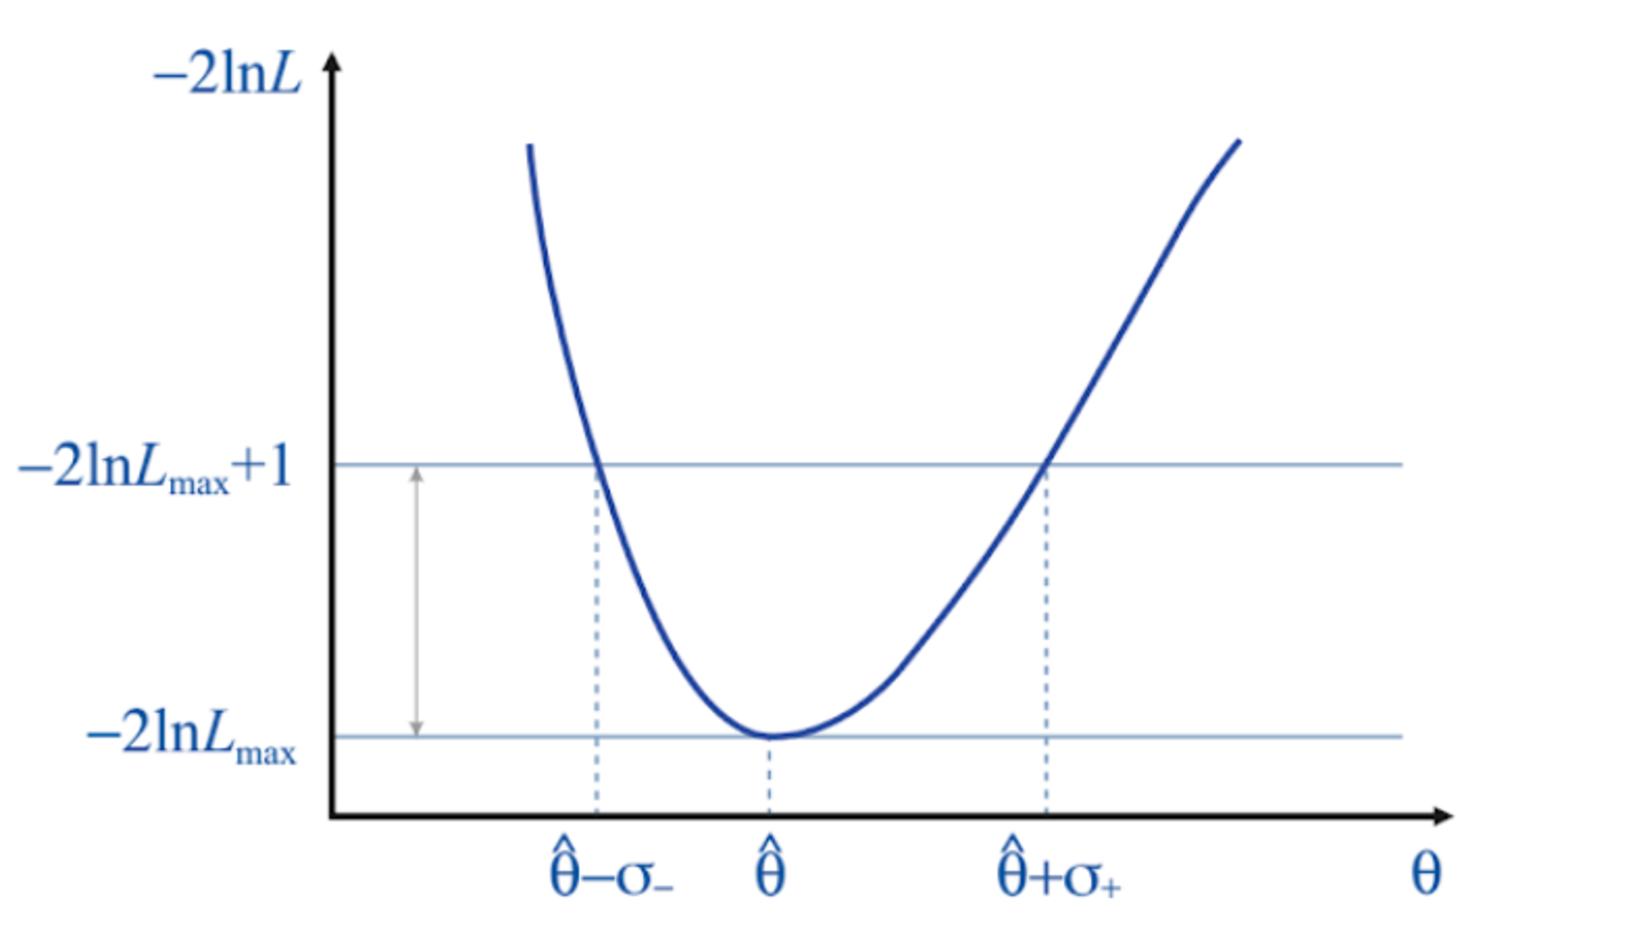
\includegraphics[width=0.7\linewidth]{figures/fitComponents/likelihood.pdf}
\caption{An illustrative example of a distribution of $-2\log L$ as a function of the parameter $\theta$. The uncertainty is determined by the variation in $-2\log L$ about the minimum.}
\label{fig:likelihood}
\end{figure}

\Fig\ref{fig:likelihood} illustrates $-2\log L$ as a function of a single parameter as an example, however, this procedure usually involves a multi-dimensional minimisation being performed. Additionally, a model is often constructed which contains multiple PDFs. Due to the complexity of the problem, the minimisation is performed using numerical methods~\cite{minuit}.


\subsection{Signal shape}
\label{sec:massfit:signal}

A single Gaussian is not sufficient to model the signal shape in \Bm mass as the detector resolution is not straightforward, it varies with momentum and location of the tracks within the detector. Therefore the shape is described as the sum of two Gaussians, each with a tail extending towards lower invariant mass to account for radiative effects. These modified Gaussians are known as Crystal Ball (CB) functions~\cite{Skwarnicki:1986xj}. The so-called Double Crystal Ball (DCB) shape is defined as a function of reconstructed mass, $m$, by
\begin{equation}
\mathrm{DCB}(m| \mu,\sigma,\alpha,n,f_{\sigma}) = f_{cb} \cdot \mathrm{CB}(m| \mu,\sigma,\alpha,n) + (1-f_{cb}) \cdot \mathrm{CB}(m|\mu,f_{\sigma}\sigma,\alpha,n),
\label{DCBshape}
\end{equation}
where
\begin{equation*}
  \mathrm{CB}(m| \mu,\sigma,\alpha,n)=
\begin{cases}
    e^{-((m-\mu)/ \sigma)^2/2},                                   & \text{if } \frac{m-\mu}{\sigma} \geq - \alpha, \\
   \left ( \frac{n}{|\alpha|} \right ) ^n e^{-|\alpha|^2/2} \left ( \frac{n}{|\alpha|} - |\alpha| - \left ( \frac{m-\mu}{\sigma} \right ) \right ) ^{-n} ,    & \text{otherwise.}
\end{cases}
\end{equation*}
Here $\mu$ is the peak position, $\sigma$ is the width of the Gaussian, $n$ parameterises the power-law tail, which starts $\alpha\sigma$ away from the peak position. The parameters $f_{cb}$ and $(1-f_{cb})$ are the fractions of the yield given to each CB, and $f_{\sigma}$ is the ratio of the widths between the two CBs. The signal PDF, $P_{sig}(m)$, must be normalised to unity with normalisation constant, $\mathcal{K}_{sig}$, such that
\begin{equation}
P_{sig}(m) = \mathcal{K}_{sig} . DCB(m| \mu,\sigma,\alpha,n,f_{\sigma}) \text{ ,	where } \int_{m_0}^{m_1} P_{sig}(m)\ dm = 1 \text{ , }
\end{equation}
and $m_0$ and $m_1$ are the lower and upper limits of the mass fit, respectively.

The \Bm mass distributions from simulated signal events are found to be consistent between \runone and \runtwo data samples, but slightly different for \kpi and \kpipipi modes. Therefore the signal shape for different data-taking periods is the same, but different between \kpi and \kpipipi modes. 

Unbinned maximum likelihood fits are performed to simulated signal samples, as shown in \fig\ref{signalfits}, and the shape parameters obtained from these fits are detailed in \tab\ref{signalparameters}. The residuals in these plots are defined as the difference between the data and the projection of the PDF in the centre of the bin, divided by the Poisson error on the number of candidates in that bin. The tail parameters, $\alpha$ and $n$, are highly correlated, therefore in order to prevent arbitrary variations between the two parameters and to ensure a stable fit, $n$ is fixed in the fits to the simulated samples. The variation in this parameter does not have significant effect on the quality of the fit, therefore $n$ is fixed to unity. For the fit to data, in addition to $n$, the tail parameter $\alpha$ and the ratio of the widths between the CBs, $f_{\sigma}$, are fixed from simulation. However, it is necessary to allow for some variation in the signal shape when performing the fit to data, as parameters, such as the peak position and width, may take slightly different values in data due to imperfections in the simulation of reconstruction and resolution effects of the \lhcb detector. Therefore, the peak position and width, $\mu$ and $\sigma$, are allowed to vary.

\begin{figure}[h]
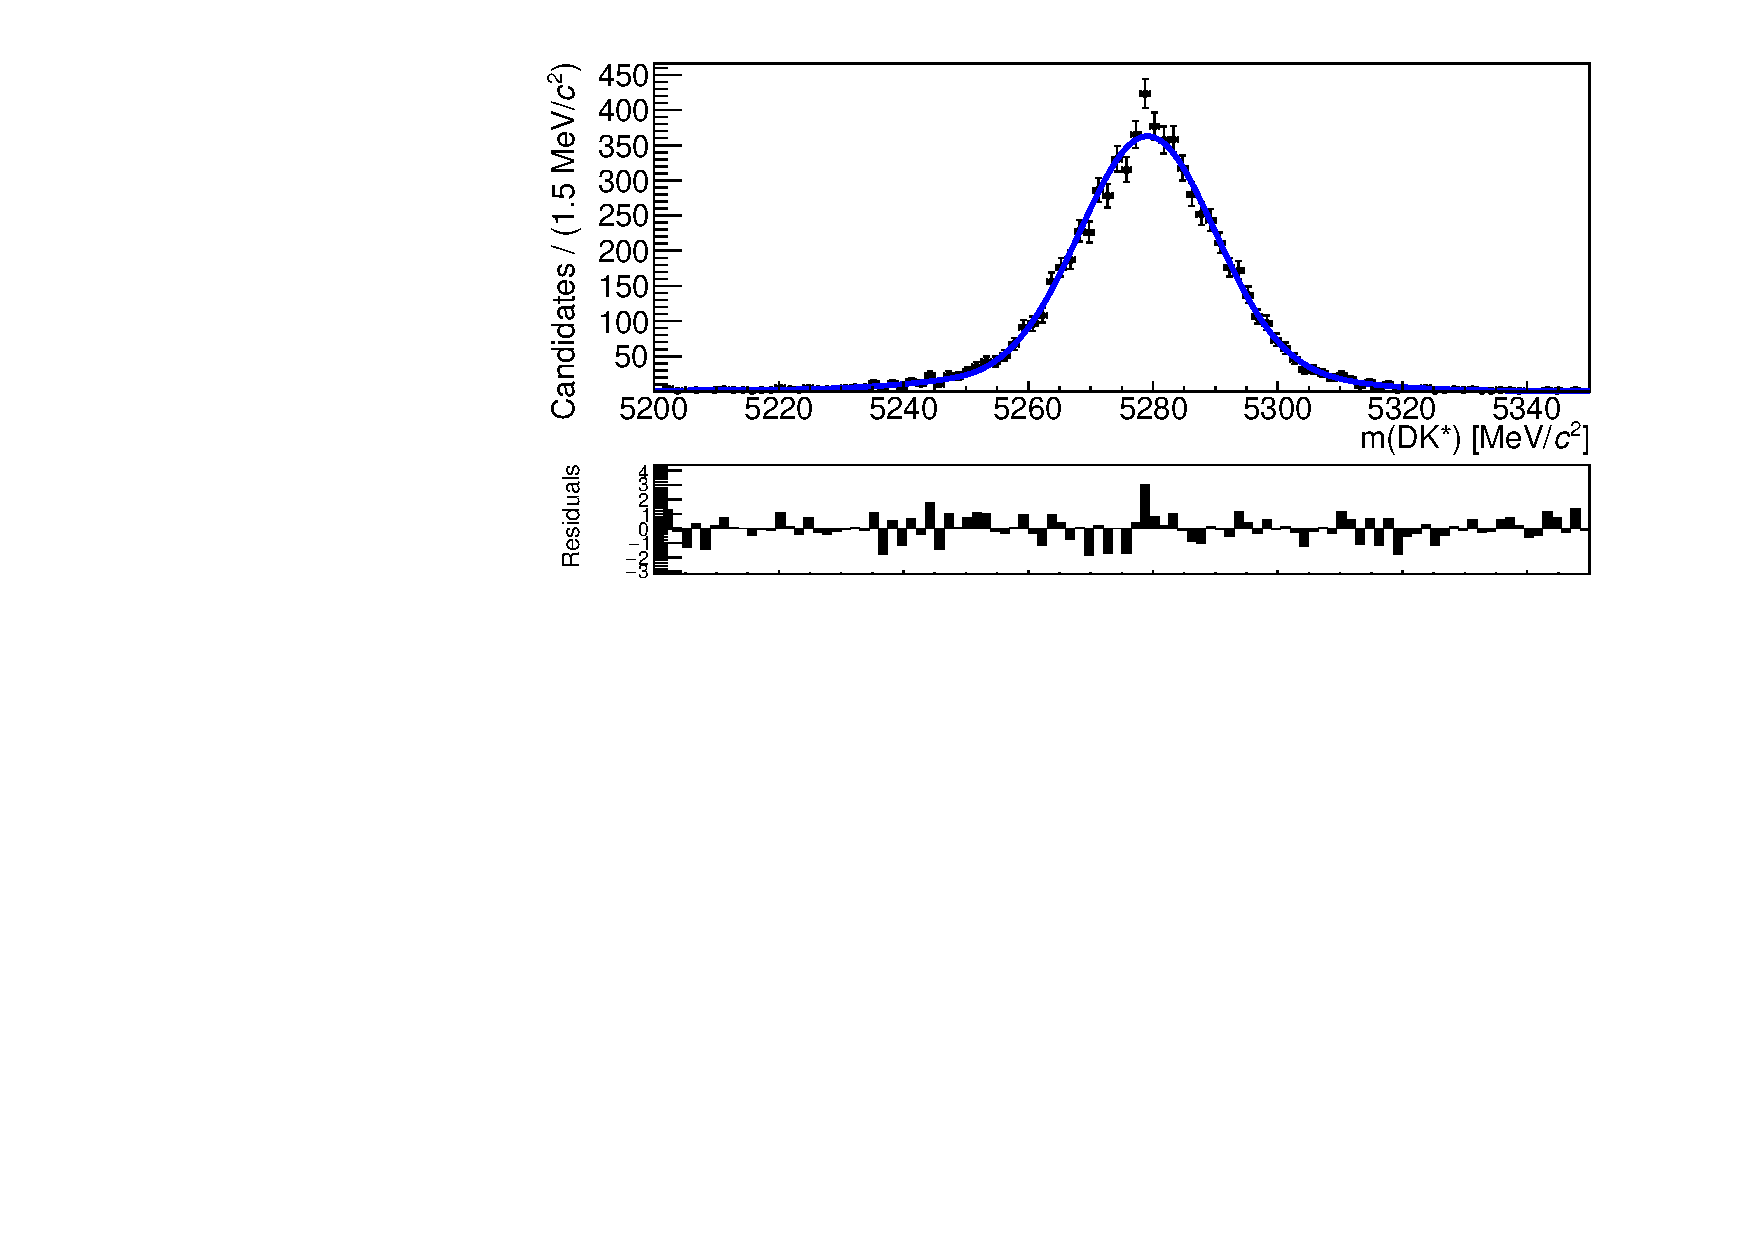
\includegraphics[width=0.5\linewidth]{figures/fitComponents/signalShape_LL_KPi.pdf}
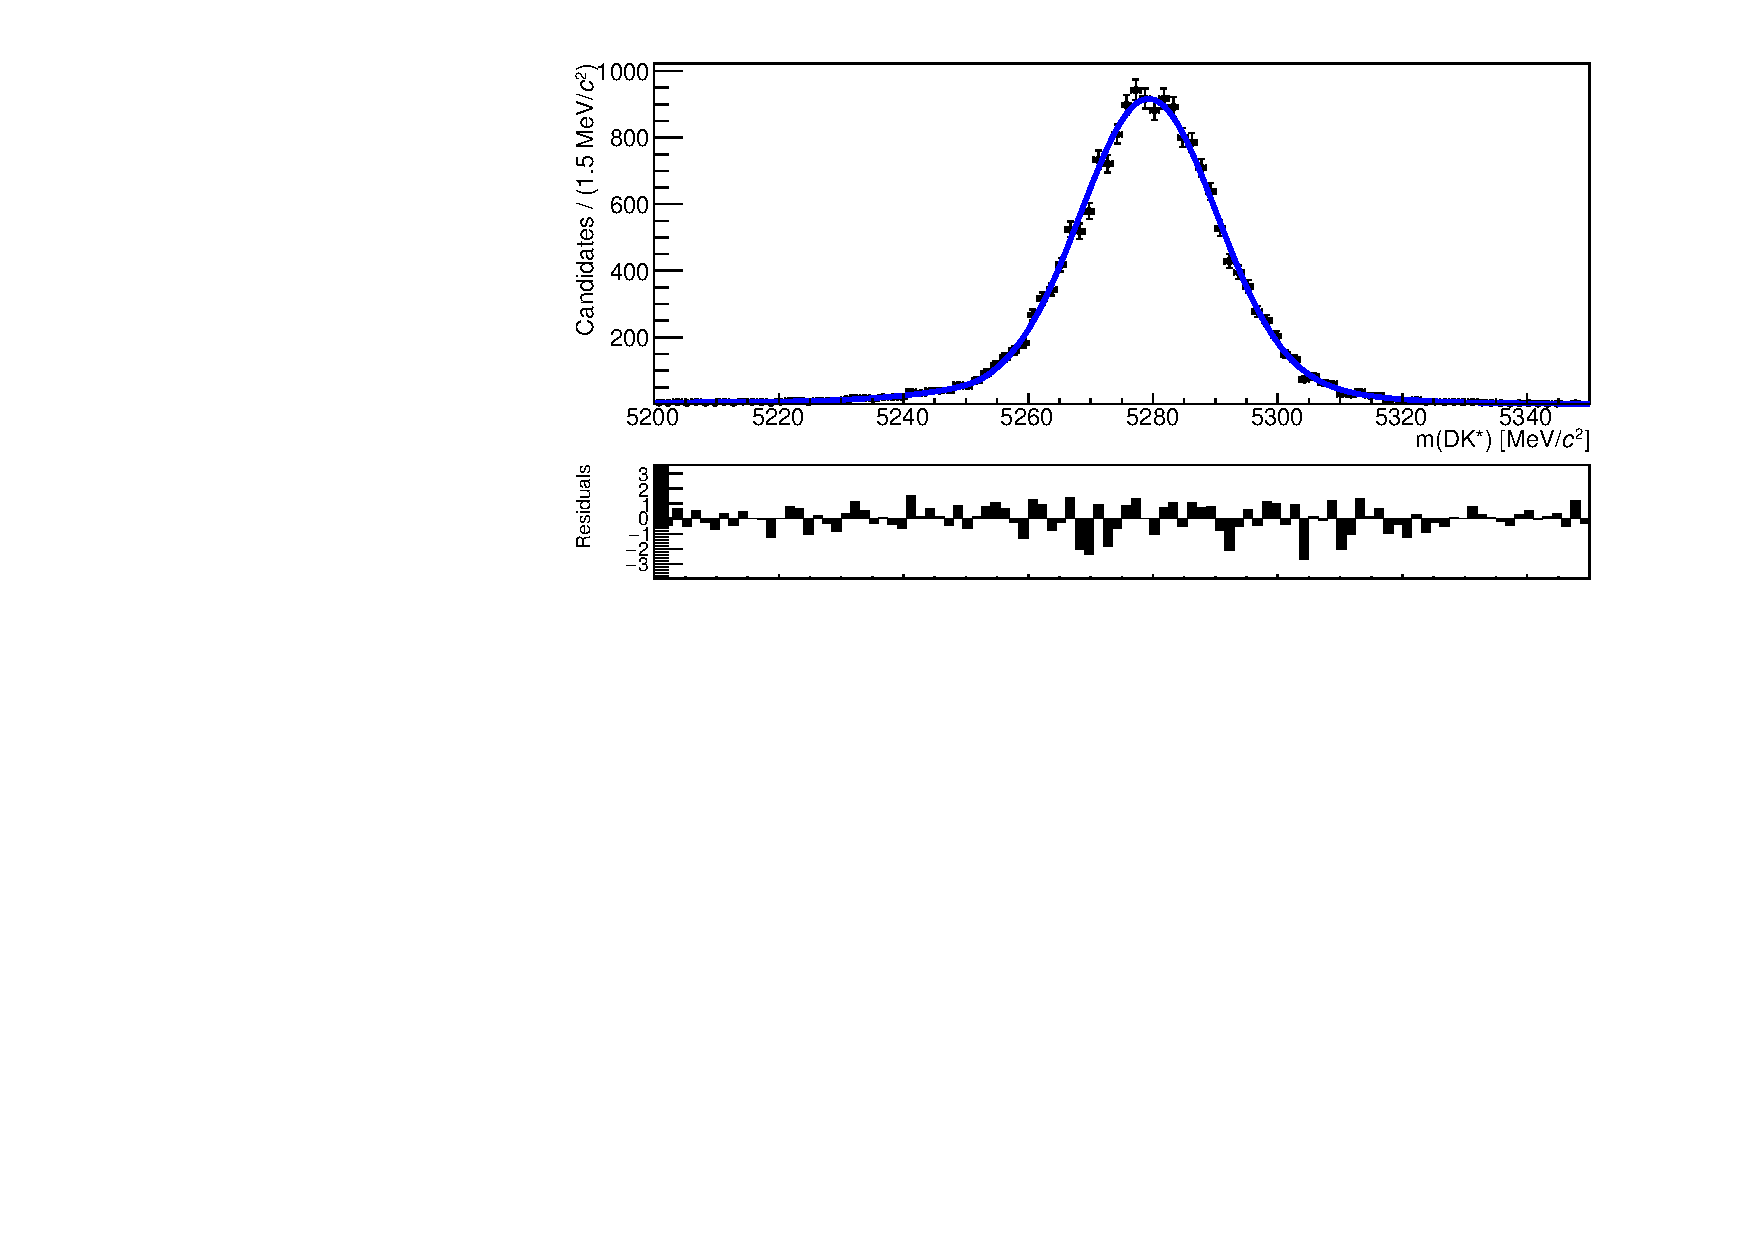
\includegraphics[width=0.5\linewidth]{figures/fitComponents/signalShape_DD_KPi.pdf}
\put(-390,70) {(a)}
\put(-180,70) {(b)}
\hfill
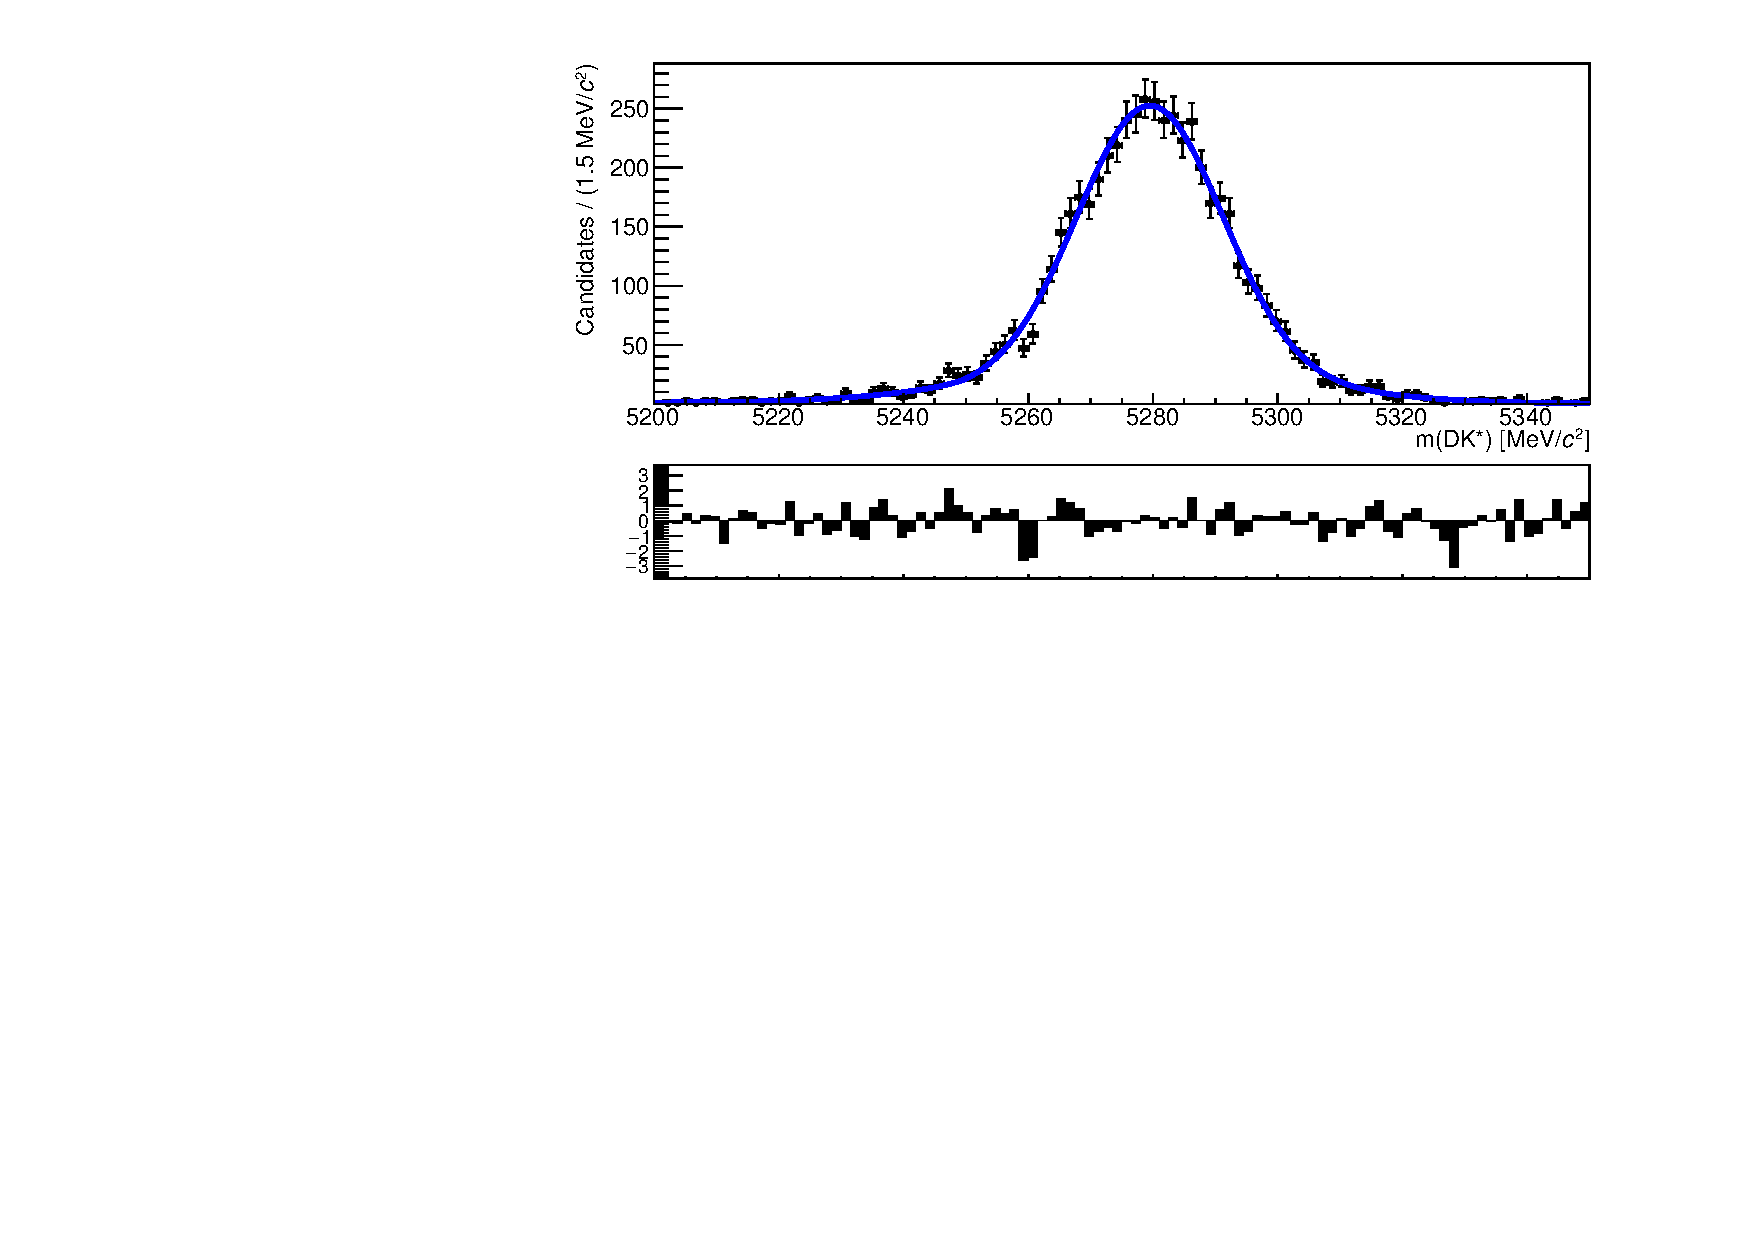
\includegraphics[width=0.5\linewidth]{figures/fitComponents/signalShape_LL_KPiPiPi.pdf}
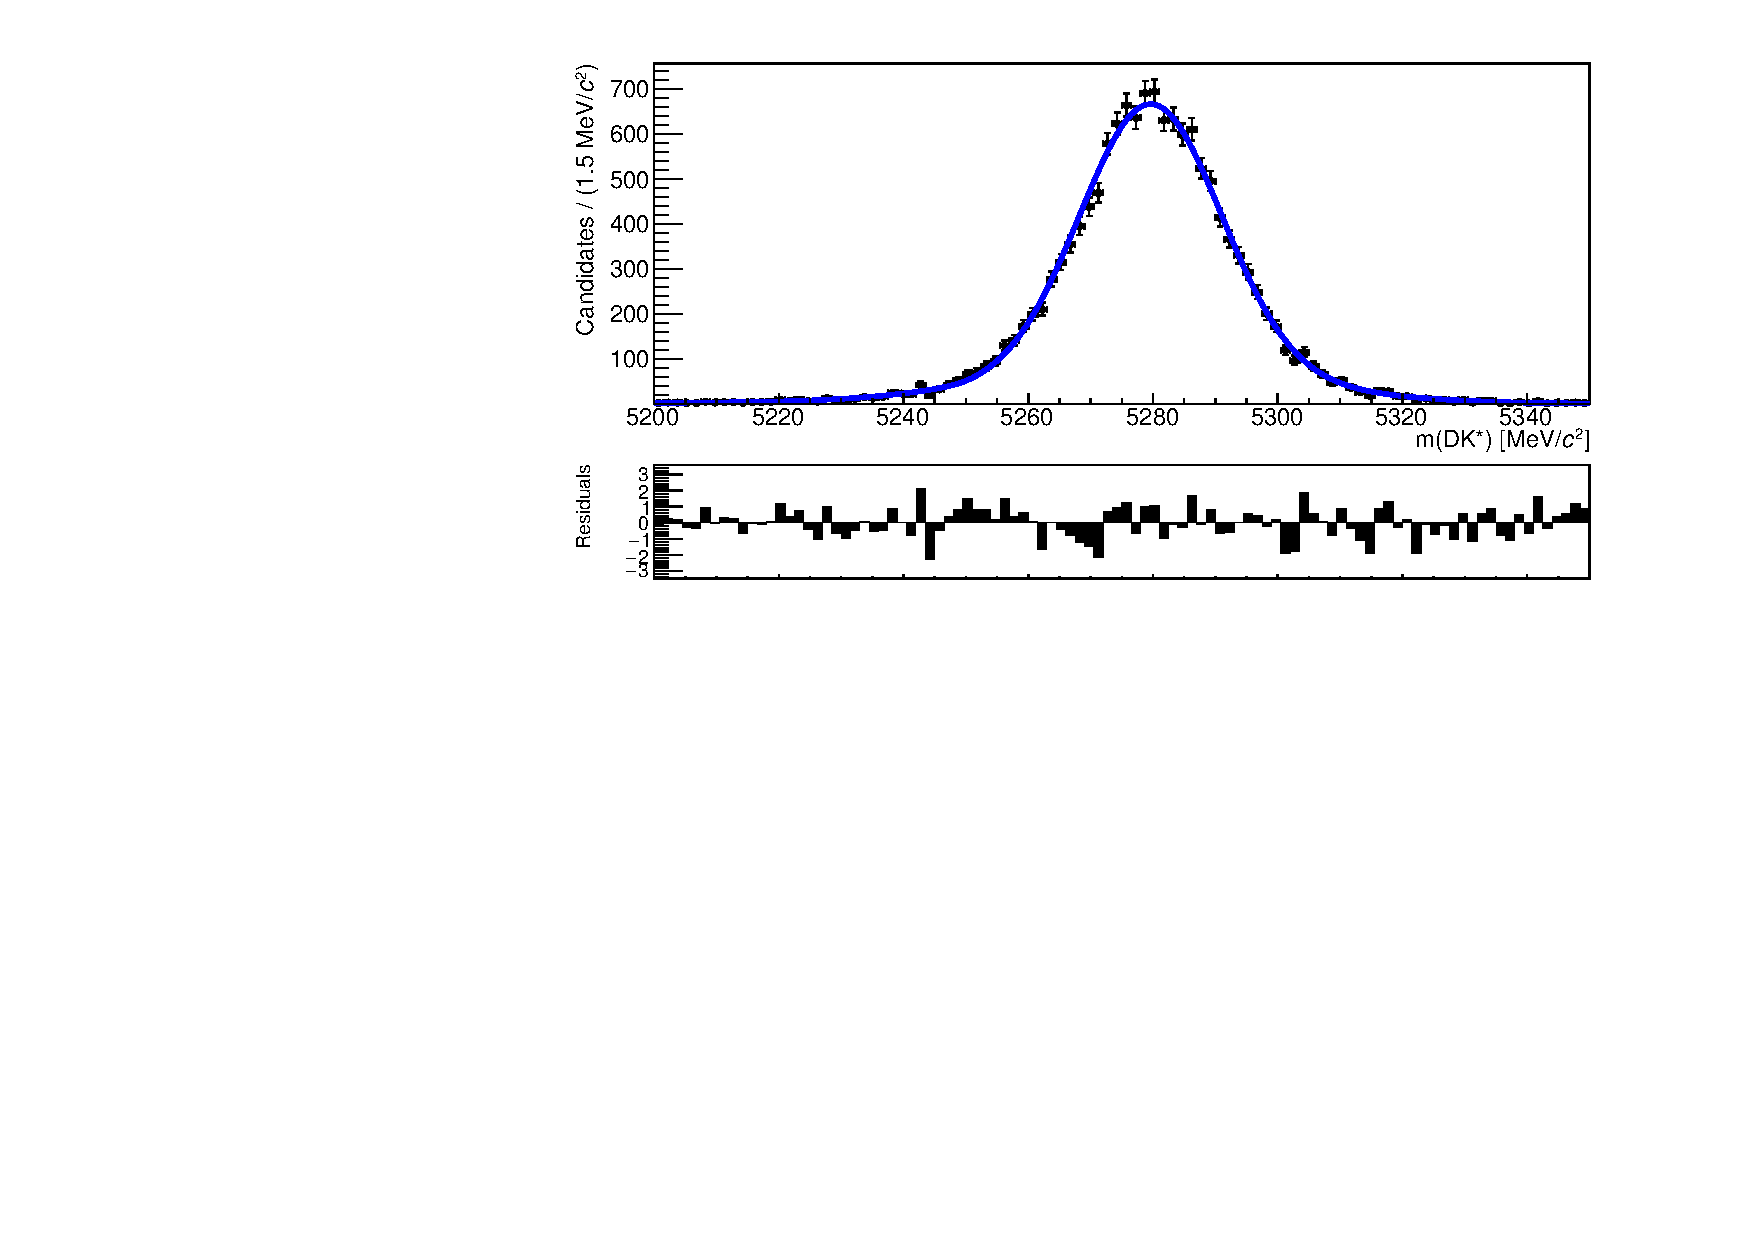
\includegraphics[width=0.5\linewidth]{figures/fitComponents/signalShape_DD_KPiPiPi.pdf}
\put(-390,70) {(c)}
\put(-180,70) {(d)}
\caption{Results of the unbinned maximum likelihood fits to the \Bm mass distribution from simulated signal samples with \runone and \runtwo data combined for (a) \kpi LL, (b) \kpi DD, (c) \kpipipi LL, and (d) \kpipipi DD. The black points represent the data, while the blue curve is the projection of the optimised shape of the form given in \eqn\ref{DCBshape}. The residuals are shown at the bottom of each plot.}
\label{signalfits}
\end{figure}

\begin{table}[h]
\centering
\begin{tabular}{c|cc|cc}
\hline
& \multicolumn{2}{c}{\kpi} & \multicolumn{2}{c}{\kpipipi} \\
& LL & DD & LL & DD\\
\hline
$\mu/\mevcc$ & $5279.12 \pm 0.15$ & $5279.30 \pm 0.09$ & $5279.62 \pm 0.12$ & $5279.50 \pm 0.19$ \\
$\sigma/\mevcc$ & $10.7 \pm 0.3$ & $10.8 \pm 0.2$ & $11.2 \pm 0.2$ & $11.6 \pm 0.3$ \\
$f_{\sigma}$ & $2.04 \pm 0.10$ & $1.97 \pm 0.06$ & $2.08 \pm 0.07$ & $2.10 \pm 0.11$ \\
$\alpha$ & $2.53 \pm 0.07$ & $2.46 \pm 0.04$ & $2.60 \pm 0.07$ & $2.50 \pm 0.10$ \\
$n$ & 1.0 (fixed) & 1.0 (fixed) & 1.0 (fixed) & 1.0 (fixed) \\
$f_{cb}$ & $0.82 \pm 0.03$ & $0.84 \pm 0.02$ & $0.80 \pm 0.03$ & $0.81 \pm 0.04	$ \\
\hline
\end{tabular}
\caption{Signal shape parameters obtained by a fit to simulated signal samples of the \kpi and \kpipipi modes with \runone and \runtwo samples combined. Parameter names are defined in \eqn\ref{DCBshape}. All parameters except for the peak position and width are fixed to these values in the mass fit.}
\label{signalparameters}
\end{table}


\subsection{Combinatorial background}
\label{sec:massfit:combinatorial}

The combinatorial background is formed of random tracks, that do not correspond to the signal decay, being combined in the reconstruction. 
%Examples of this background include, random kaon and pion tracks in the detector incorrectly reconstructed to form a \Dz meson, real reconstructed \Dz mesons combined with a random \KS meson, or random pion tracks combined to make a incorrectly reconstructed \KS meson. 
The combinatorial background is modelled using an exponential PDF, $P_{bkg}$, given by
\begin{equation}
P_{bkg} = \mathcal{K}_{bkg}\ e^{\beta m} \text{ , \hspace{5pt} with } \mathcal{K}_{bkg} = \frac{\beta}{e^{\beta m_1} - e^{\beta m_0}} \text{ , }
\label{combpdf}
\end{equation}
and where $m_0$ and $m_1$ are the lower and upper limits of the mass fit, respectively, and $\beta$ is the slope parameter that is allowed to vary. 


%%%%%%%%%%%%%%%%%%%%%%
\subsection{Partially reconstructed backgrounds}
\label{sec:massfit:partreco}

Partially reconstructed decays refer to those in which one or more particle, in a \B decay similar to the signal decay, has failed to be reconstructed, resulting in peaking structures in the \B mass spectrum at a reconstructed mass lower than the signal peak. The partially reconstructed decays are of the form \decay{\B}{\Dstar\Kstar}, where the \Dstar decays to a \Dz meson and a pion or photon that is missed when reconstructing the decay. Three partially reconstructed decays contribute to the invariant mass fit:

\begin{itemize}
\item{\decay{\Bm}{(\decay{\Dstarz}{\Dz[\piz]})\Kstarm},}
\item{\decay{\Bm}{(\decay{\Dstarz}{\Dz[\gamma]})\Kstarm},}
\item{\decay{\Bd}{(\decay{\Dstarp}{\Dz[\pip]})\Kstarm},}
\end{itemize}
where the particle in square brackets corresponds to the missed particle. Each \decay{\B}{\Dstar\Kstar} decay is a {\textit{Scalar $\to$ Vector Vector}} decay, therefore, due to the conservation of angular momentum, there are three different helicity amplitudes to consider, labelled +1, 0, -1 corresponding to the helicity state of the \Dstar particle. The helicity state of the \Dstar and the spin of the missing particle in the subsequent \Dstar decay determines the distribution of the reconstructed \B mass. The states +1 and -1 produce the same distribution in \Bm mass, therefore for the mass parameterisation these states are combined and collectively referred to as $\pm$1. This results in six different shapes to be modelled in the mass fit:
\begin{itemize}
\item{\decay{\Bm}{(\decay{\Dstarz}{\Dz[\piz]})\Kstarm}, \Dstarz helicity: 0,} 
\item{\decay{\Bm}{(\decay{\Dstarz}{\Dz[\piz]})\Kstarm}, \Dstarz helicity: $\pm$1,} 
\item{\decay{\Bm}{(\decay{\Dstarz}{\Dz[\gamma]})\Kstarm}, \Dstarz helicity: 0,}
\item{\decay{\Bm}{(\decay{\Dstarz}{\Dz[\gamma]})\Kstarm}, \Dstarz helicity: $\pm$1,}
\item{\decay{\Bd}{(\decay{\Dstarp}{\Dz[\pip]})\Kstarm}, \Dstarp helicity: 0,}
\item{\decay{\Bd}{(\decay{\Dstarp}{\Dz[\pip]})\Kstarm}, \Dstarp helicity: $\pm$1.}
\end{itemize}
All of these shapes are modelled using three analytic PDFs; the so-called Horns, Hill and Little Horns, developed by Paolo Gandini and Shu-Faye Cheung for the study of \decay{\Bm}{\D(hh')\Km} and \decay{\Bz}{\D\Kstarz} decays~\cite{LHCb-PAPER-2017-021,LHCb-PAPER-2016-006}. These shapes are physically motivated, exploiting the decay kinematics of the partially reconstructed decays.

\subsubsection{Horns function}

Consider the \decay{\Bm}{\Dstarz\Kstarm}, \decay{\Dstarz}{\Dz\piz}, where the \Dstarz is in helicity state 0. The helicity of the \Dstarz, the fact that the missing \piz meson is spin-0 and the requirement that angular momentum must be conserved means that the \piz meson will decay predominantly along the helicity angle $\theta = 0^{\circ}$ or $\theta = 180^{\circ}$. The distribution $\theta$ has a one-to-one correspondence with its momentum and therefore the reconstructed \Bm mass. When $\theta = 0^{\circ}$, the fraction of momentum carried by the \piz in the \Bm rest frame is at its smallest, resulting in a larger reconstructed \Bm mass. Conversely, if $\theta = 180^{\circ}$, the fraction of momentum carried by the \piz is greatest, leading to a lower reconstructed \Bm mass.

This distribution is modelled using the Horns function. The underlying kinematic distribution is a parabola, $p_{HORNS}(x)$, with kinematics end-points $a$ and $b$, determined in the fit, where
\begin{align}
p_{HORNS}(x) &= \begin{cases}
\left(x - \frac{a+b}{2}\right)^2, & \text{ if $a \leq x \leq b$}\\ 	
0, & \text{ otherwise.}
\end{cases} 
\end{align}

The reconstruction of particles within the \lhcb detector gives rise to resolution effects that result in a smearing of the mass distribution. These resolution effects are modelled by convolving the Horns parabola with two Gaussians. Given a Gaussian function of mean $m$ and width $\sigma$, $G(m,\sigma)$, a Double Gaussian can be constructed as
\begin{equation}
DG(x) = f_G G(x|m,\sigma) + \left(1-f_G\right) G(x|m,R_{\sigma}\sigma) \text{ , }
\end{equation}
where $\sigma$ is the width of the first Gaussian, $f_G$ is the fractional yield contained by the first Gaussian and $R_{\sigma}$ is the relative width between the two. Additionally selection effects, arising from preferentially selecting high \pt events, can affect the shape of one peak relative to the other. This is taken into account by introducing a linear polynomial with a slope of $1 - \xi$. The resulting Horns PDF is,
\begin{multline}
\text{Horns}(m) = \mathcal{K}_{Horns}\ \int_a^b dx \left(x - \frac{a+b}{2}\right)^2 DG(x|m,\sigma,f_G,R_{\sigma}) \\
\left( \frac{1 - \xi_{HORNS}}{b - a}x + \frac{b\xi_{HORNS} - a}{b - a}\right),
\label{eqn:horns}
\end{multline}
where $m$ is the mass variable to be fitted, $x$ is the integration variable in the convolution, and $\mathcal{K}_{Horns}$ is the normalisation constant required for the PDF. An example of such a double peak structure is shown in \fig\ref{fig:horns} for simulated data.

\begin{figure}[h]
\centering
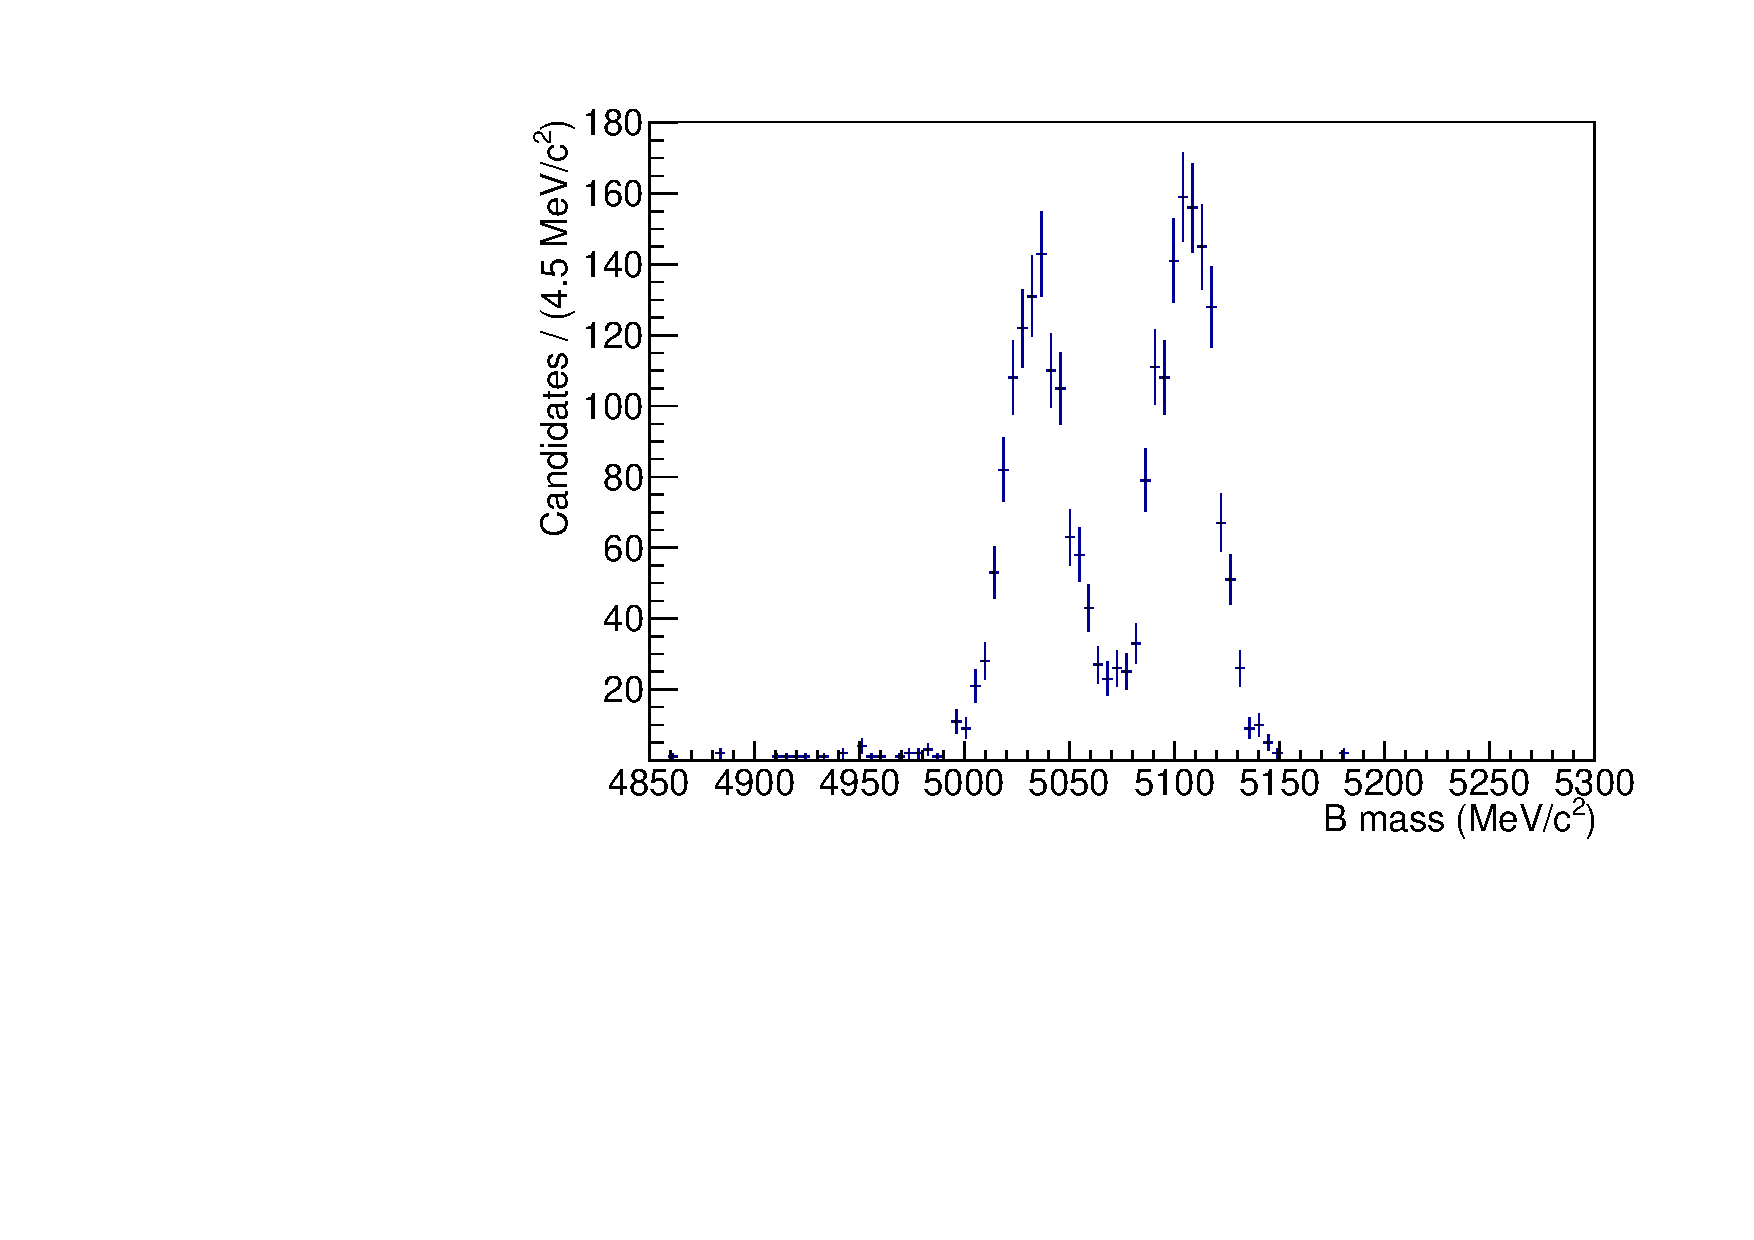
\includegraphics[width=0.5\linewidth]{figures/fitComponents/horns.pdf}
\caption{Distribution of simulated \decay{\Bm}{(\decay{\Dstarz}{\Dz\piz})\Kstarm} events, where the \piz is missed in reconstruction and the \Dstarz is in helicity state 0.}
\label{fig:horns}
\end{figure}

\subsubsection{Hill function}

Consider now the \decay{\Bm}{\Dstarz\Kstarm}, \decay{\Dstarz}{\Dz\gamma}, where the \Dstarz is in helicity state 0. The helicity of the \Dstarz, the fact that the \Pgamma is spin-1 and the requirement that angular momentum is conserved means that the \Pgamma will decay predominantly along $\theta = 90^{\circ}$ or $\theta = 270^{\circ}$. The fraction of momentum carried by the photon is the same in both cases, so no double peak structure is observed.

This distribution is modelled using the Hill function. The underlying kinematic distribution is a parabola with negative curvature, $p_{HILL}(x)$, and kinematic endpoints $a$ and $b$ where
\begin{align}
p_{HILL}(x) &= \begin{cases}
-(x - a')(x - b'), & \text{ if $a' \leq x \leq b'$}\\ 	
0, & \text{ otherwise.}
\end{cases} 
\end{align}

As with the Horns function, this parabola is convolved with a Double Gaussian and a linear polynomial to account for resolution and selection effects, respectively. The resulting Hill function is
\begin{multline}
\text{Hill}(m) = \mathcal{K}_{Hill}\ \int_{a'}^{b'} dx \left[-(x - a')(x - b')\right] DG(x|m,\sigma,f_G,R_{\sigma}) \\
\left( \frac{1 - \xi_{HILL}}{b' - a'}x + \frac{b'\xi_{HILL} - a'}{b' - a'}\right),
\label{eqn:hill}
\end{multline}
where $m$ is the mass variable to be fitted, $x$ is the integration variable in the convolution and $\mathcal{K}_{Hill}$ is the normalisation constant required for the PDF. This Hill function also applies to the \decay{\Bm}{\Dstarz\Kstarm}, \decay{\Dstarz}{\Dz\piz} decay, where the \Dstarz is in helicity state $\pm$1. An example of such a distribution is shown in \fig\ref{fig:hill} for simulated data.

\begin{figure}[h]
\centering
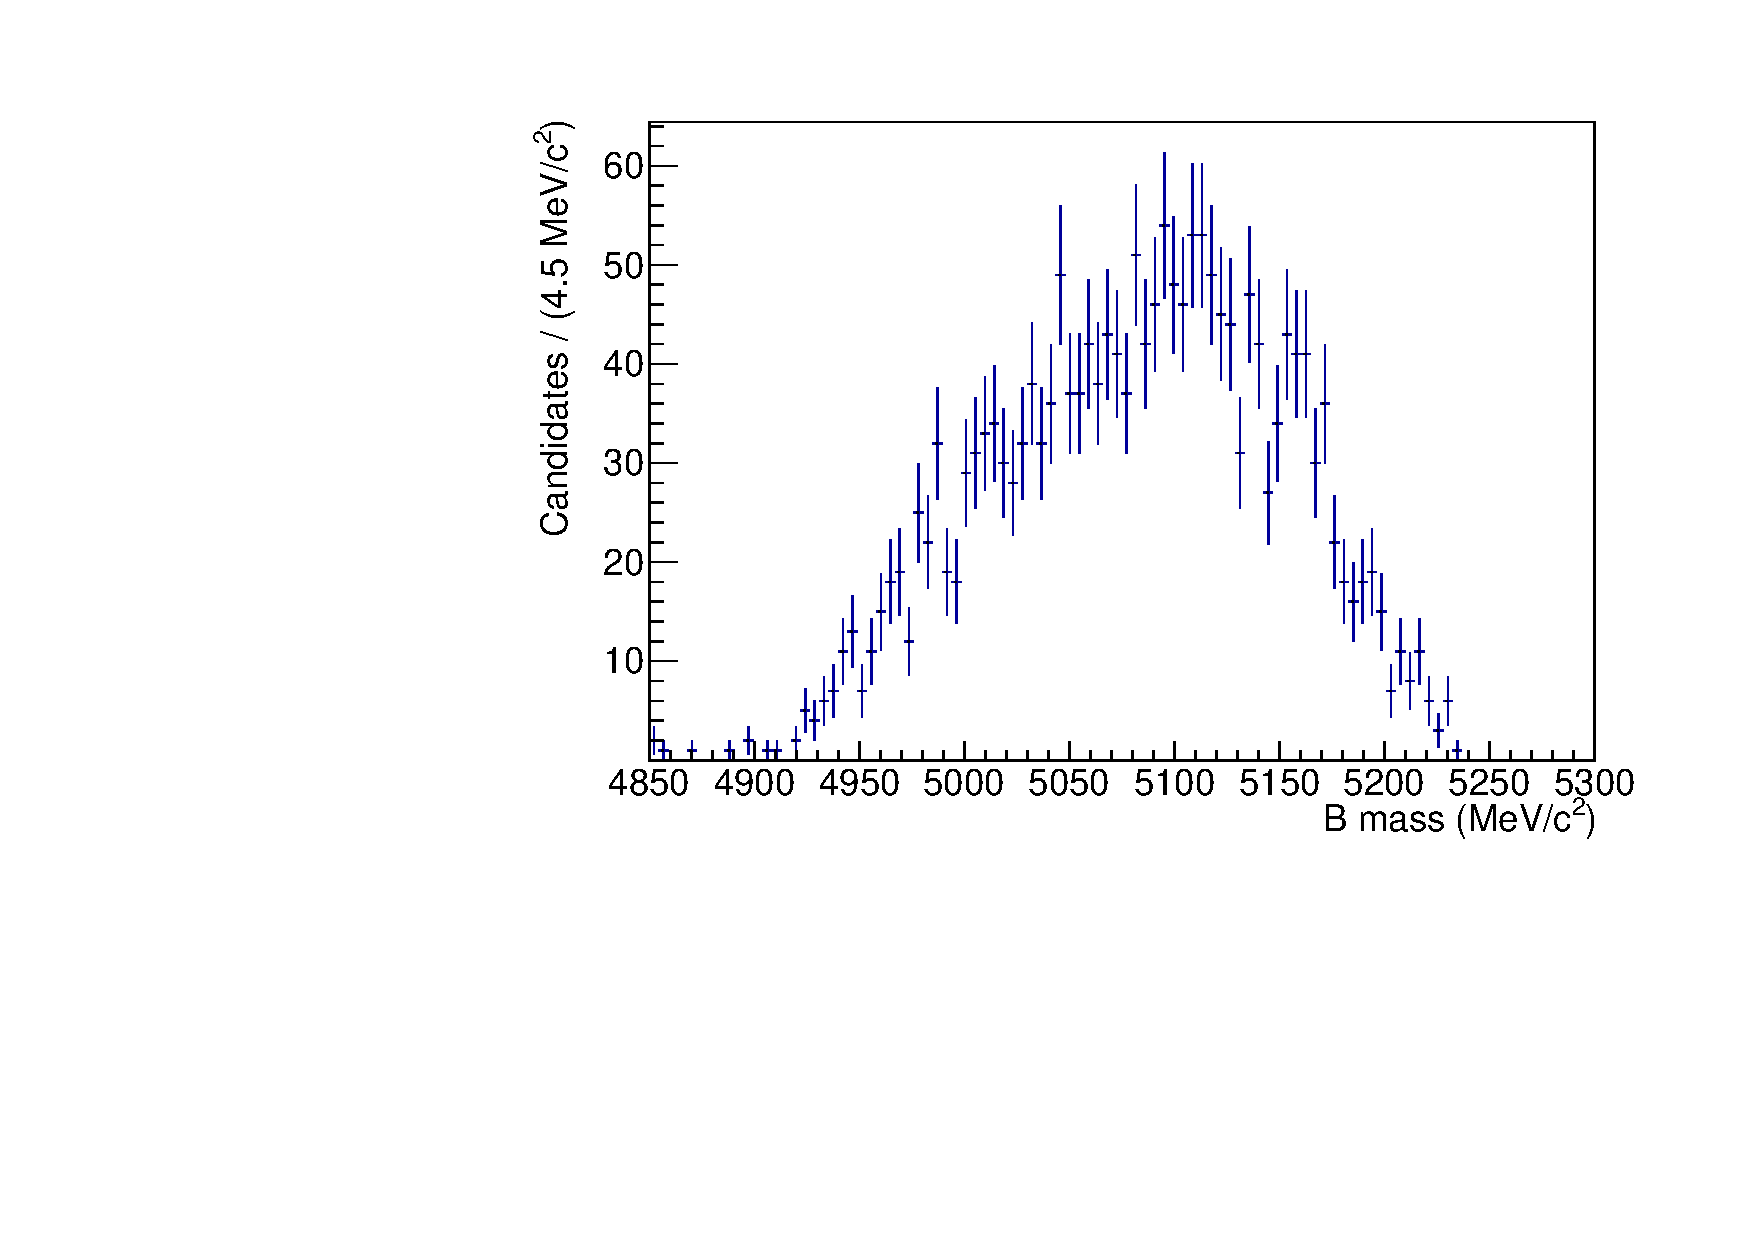
\includegraphics[width=0.5\linewidth]{figures/fitComponents/hill.pdf}
\caption{Distribution of simulated \decay{\Bm}{(\decay{\Dstarz}{\Dz\gamma})\Kstarm} events, where the \Pgamma is missed in reconstruction and the \Dstarz is in helicity state 0.}
\label{fig:hill}
\end{figure}

\subsubsection{Little Horns function}

For the configuration \decay{\Bm}{\Dstarz\Kstarm}, \decay{\Dstarz}{\Dz\gamma}, where the \Dstarz is in helicity state $\pm$1, the \Bm mass distribution is shown in \fig\ref{fig:littlehorns}.

\begin{figure}[h]
\centering
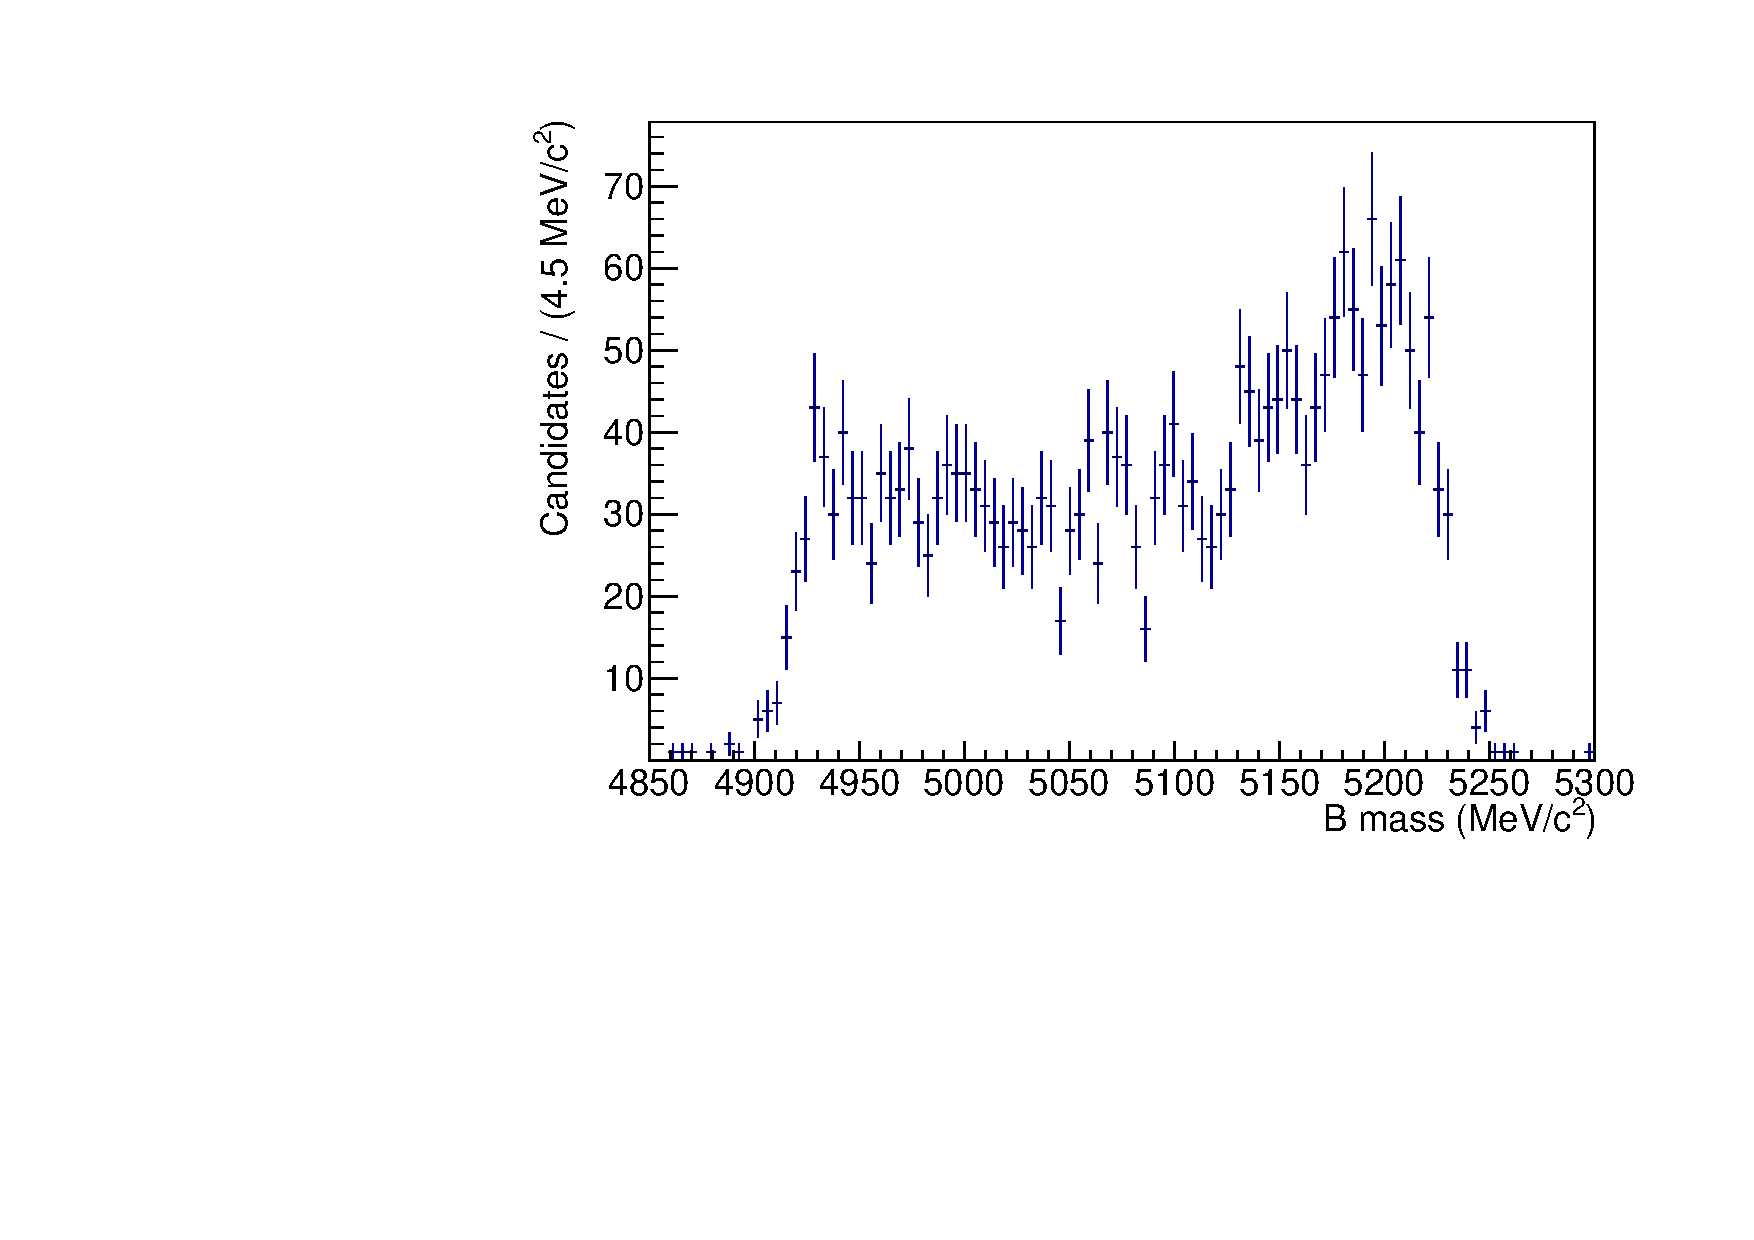
\includegraphics[width=0.5\linewidth]{figures/fitComponents/littlehorns.pdf}
\caption{Distribution of simulated \decay{\Bm}{(\decay{\Dstarz}{\Dz\gamma})\Kstarm} events, where the \Pgamma is missed in reconstruction and the \Dstarz is in helicity state $\pm$1.}
\label{fig:littlehorns}
\end{figure}
This is modelled using the Little Horns shape. The underlying kinematic distribution is described by the sum of a parabola and a uniform distribution, $p_{LITTLEHORNS}(x)$, and kinematic endpoints $a''$ and $b''$ where
\begin{align}
p_{LITTLEHORNS}(x) &= \begin{cases}
\left(x - \frac{a''+b''}{2}\right)^2 + \left(\frac{a''-b''}{2}\right)^2, & \text{ if $a'' \leq x \leq b''$}\\ 	
0, & \text{ otherwise.}
\end{cases} 
\end{align}

Again, this distribution is convolved with a Double Gaussian and linear polynomial to describe the resolution and selection effects, respectively. This results in a Little Horns function
\begin{multline}
\text{LittleHorns}(m) = \mathcal{K}_{LittleHorns}\ \int_{a''}^{b''} dx \biggl\{ \left[ \left( x - \frac{a''+b''}{2} \right) ^2 + \left( \frac{a''-b''}{2} \right) ^2 \right] \\
 DG(x|m,\sigma,f_G,R_{\sigma}) \left( \frac{1 - \xi_{LITTLEHORNS}}{b'' - a''}x + \frac{b''\xi_{LITTLEHORNS} - a''}{b'' - a''} \right) \biggr\} \text{ ,}
\label{eqn:littlehorns}
\end{multline}
where $m$ is the mass variable to be fitted, $x$ is the integration variable in the convolution and $\mathcal{K}_{LittleHorns}$ is the normalisation constant required for the PDF.

\subsubsection{Total partially reconstructed function}

The normalisation constants $\mathcal{K}_{Horns}$, $\mathcal{K}_{Hill}$ and $\mathcal{K}_{LittleHorns}$ in \eqns\ref{eqn:horns}, \ref{eqn:hill} and \ref{eqn:littlehorns} respectively, are required for the PDFs to be correctly normalised. This requires, $\int_{m_0}^{m_1} P(m) dm = 1$ for each of the PDFs, $P(m)$, where $m_0$ and $m_1$ are the lower and upper limits of the mass fit. Due to the complexity of the shapes, the normalisation constant is calculated numerically. 

Each partially reconstructed shape contributes to the mass fit in the \Bm mass region below the signal peak. \Tab\ref{helicityamplitudes} summarises the use of the different analytic shapes described: Horns, Hill and Little Horns functions. 

\begin{table}[h]
\centering
\resizebox{\textwidth}{!}{
\begin{tabular}{cccc}
Decay mode & Helicity of \Dstar & $\theta$ dependence & PDF \\
\hline
\decay{\Bm}{(\decay{\Dstarz}{\Dz[\piz]})\Kstarm} & 0 & $\left(x - \frac{a_1+b_1}{2}\right)^2$ & Horns, from \eqn\ref{eqn:horns} \\
\decay{\Bm}{(\decay{\Dstarz}{\Dz[\piz]})\Kstarm} & $\pm$1 & $-(x - a_2)(x - b_2)$ & Hill, from \eqn\ref{eqn:hill} \\
\decay{\Bm}{(\decay{\Dstarz}{\Dz[\gamma]})\Kstarm} & 0 & $-(x - a_3)(x - b_3)$ & Hill, from \eqn\ref{eqn:hill} \\
\decay{\Bm}{(\decay{\Dstarz}{\Dz[\gamma]})\Kstarm} & $\pm$1 & $\left(x - \frac{a_4+b_4}{2}\right)^2 + \left(\frac{a_4-b_4}{2}\right)^2$ & Little Horns, from \eqn\ref{eqn:littlehorns} \\
\decay{\Bz}{(\decay{\Dstarp}{\Dz[\pip]})\Kstarm} & 0 & $\left(x - \frac{a_5+b_5}{2}\right)^2$ & Horns, from \eqn\ref{eqn:horns} \\
\decay{\Bz}{(\decay{\Dstarp}{\Dz[\pip]})\Kstarm} & $\pm$1 & $-(x - a_6)(x - b_6)$ & Hill, from \eqn\ref{eqn:hill} \\
\end{tabular}}
\caption{The different partially reconstructed shapes for the \Dstar helicity states. The kinematic endpoints $a_i$ and $b_i$ can be different for each of the partially reconstructed shapes.}
\label{helicityamplitudes}
\end{table}

In order to obtain values for the various parameters in the shape functions, simulated samples are generated and the full reconstruction and selection applied. The parameters are obtained from performing individual unbinned maximum likelihood fits to the simulated samples using the functions given by \eqns\ref{eqn:horns}, \ref{eqn:hill} and \ref{eqn:littlehorns}. The fits for DD events are shown in \fig\ref{partrecofitsDD}, those for the LL samples are similar. All shape parameters are then fixed to these values for the fits to data. Although the simulated samples forced the \Dz meson to decay to \Km\pip, the \Dz meson decay mode does not have a significant effect on the shape of the partially reconstructed background, hence the same shapes are used for all \Dz decay modes. Similarly, distributions in \Bm mass of \runone and \runtwo simulated samples are considered sufficiently similar to use the same shapes for both data-taking periods.

%\begin{figure}[h]
%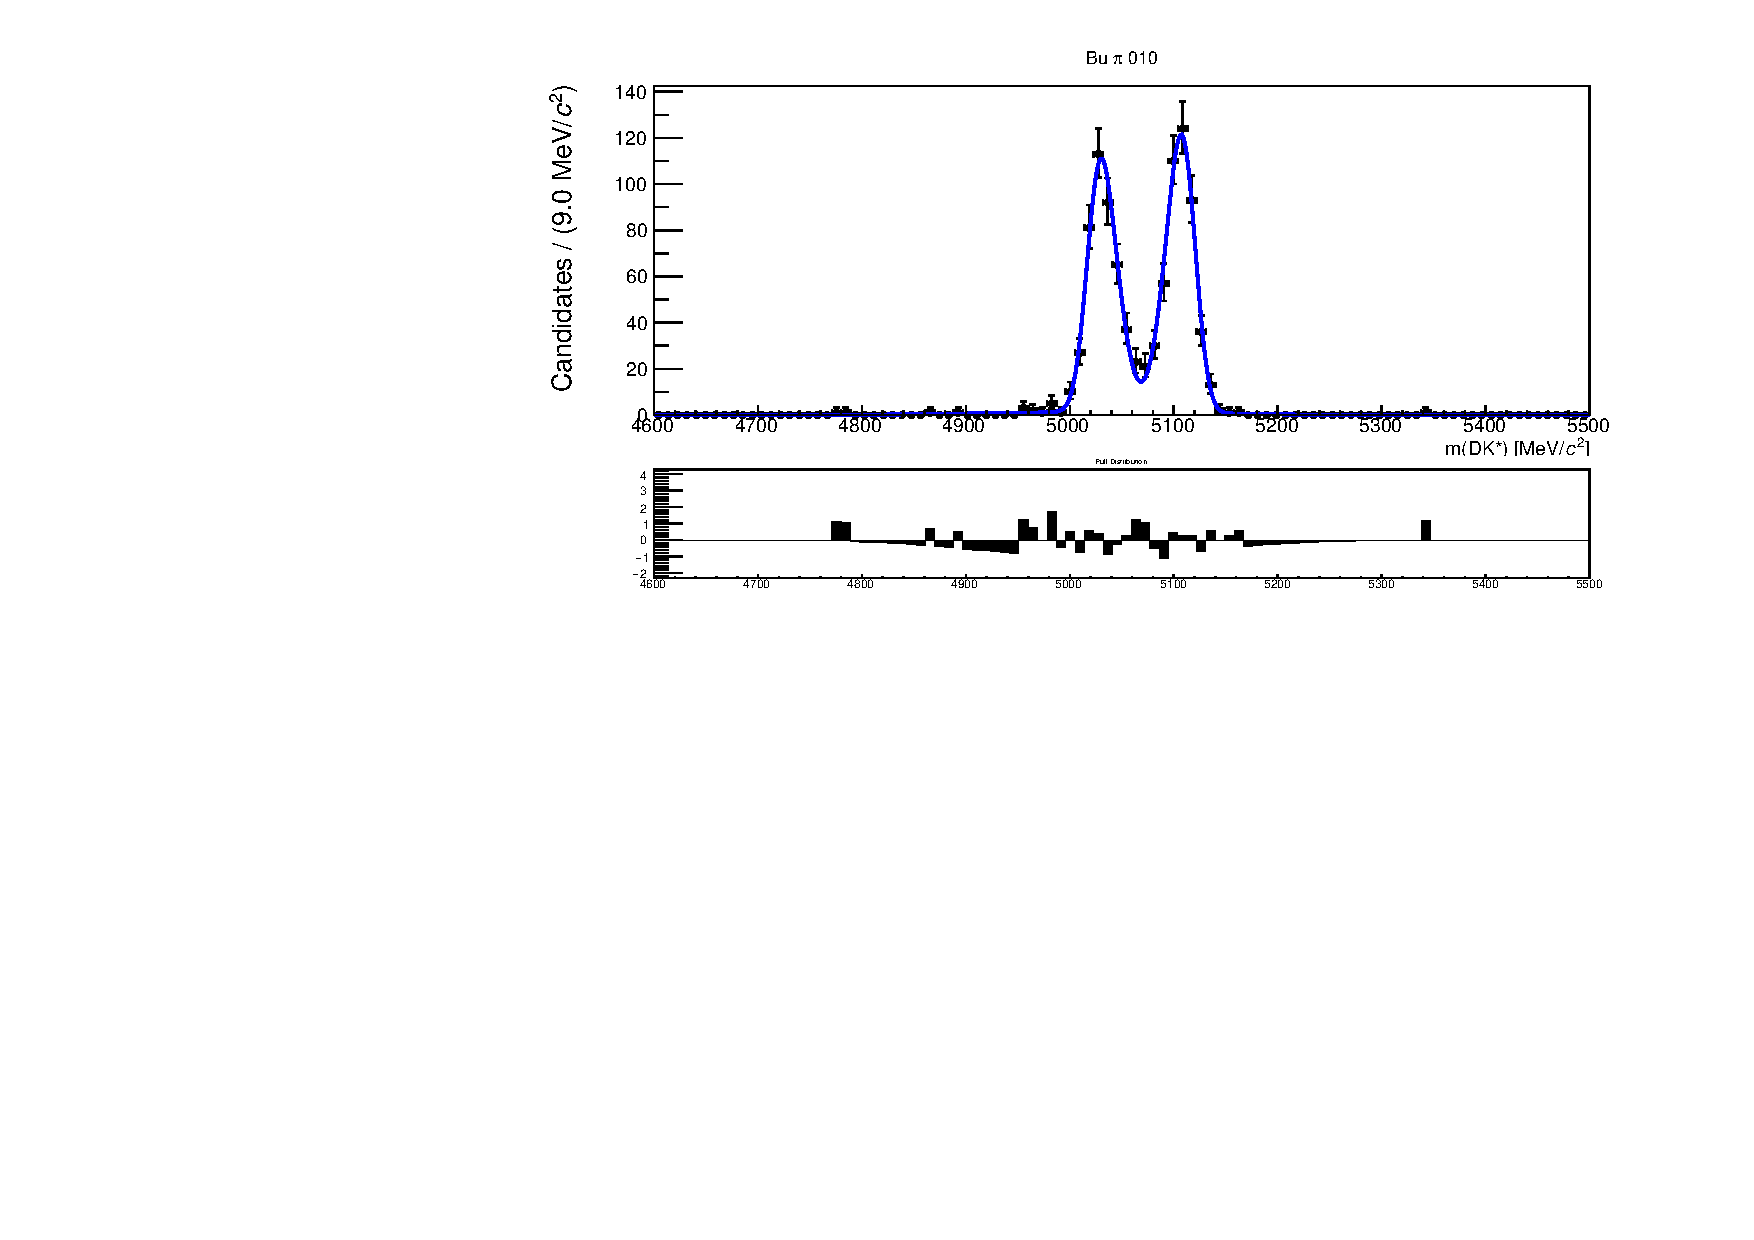
\includegraphics[width=0.5\linewidth]{figures/fitComponents/Bupi010_LL.pdf}
%\put(-170,70) {(a)}
%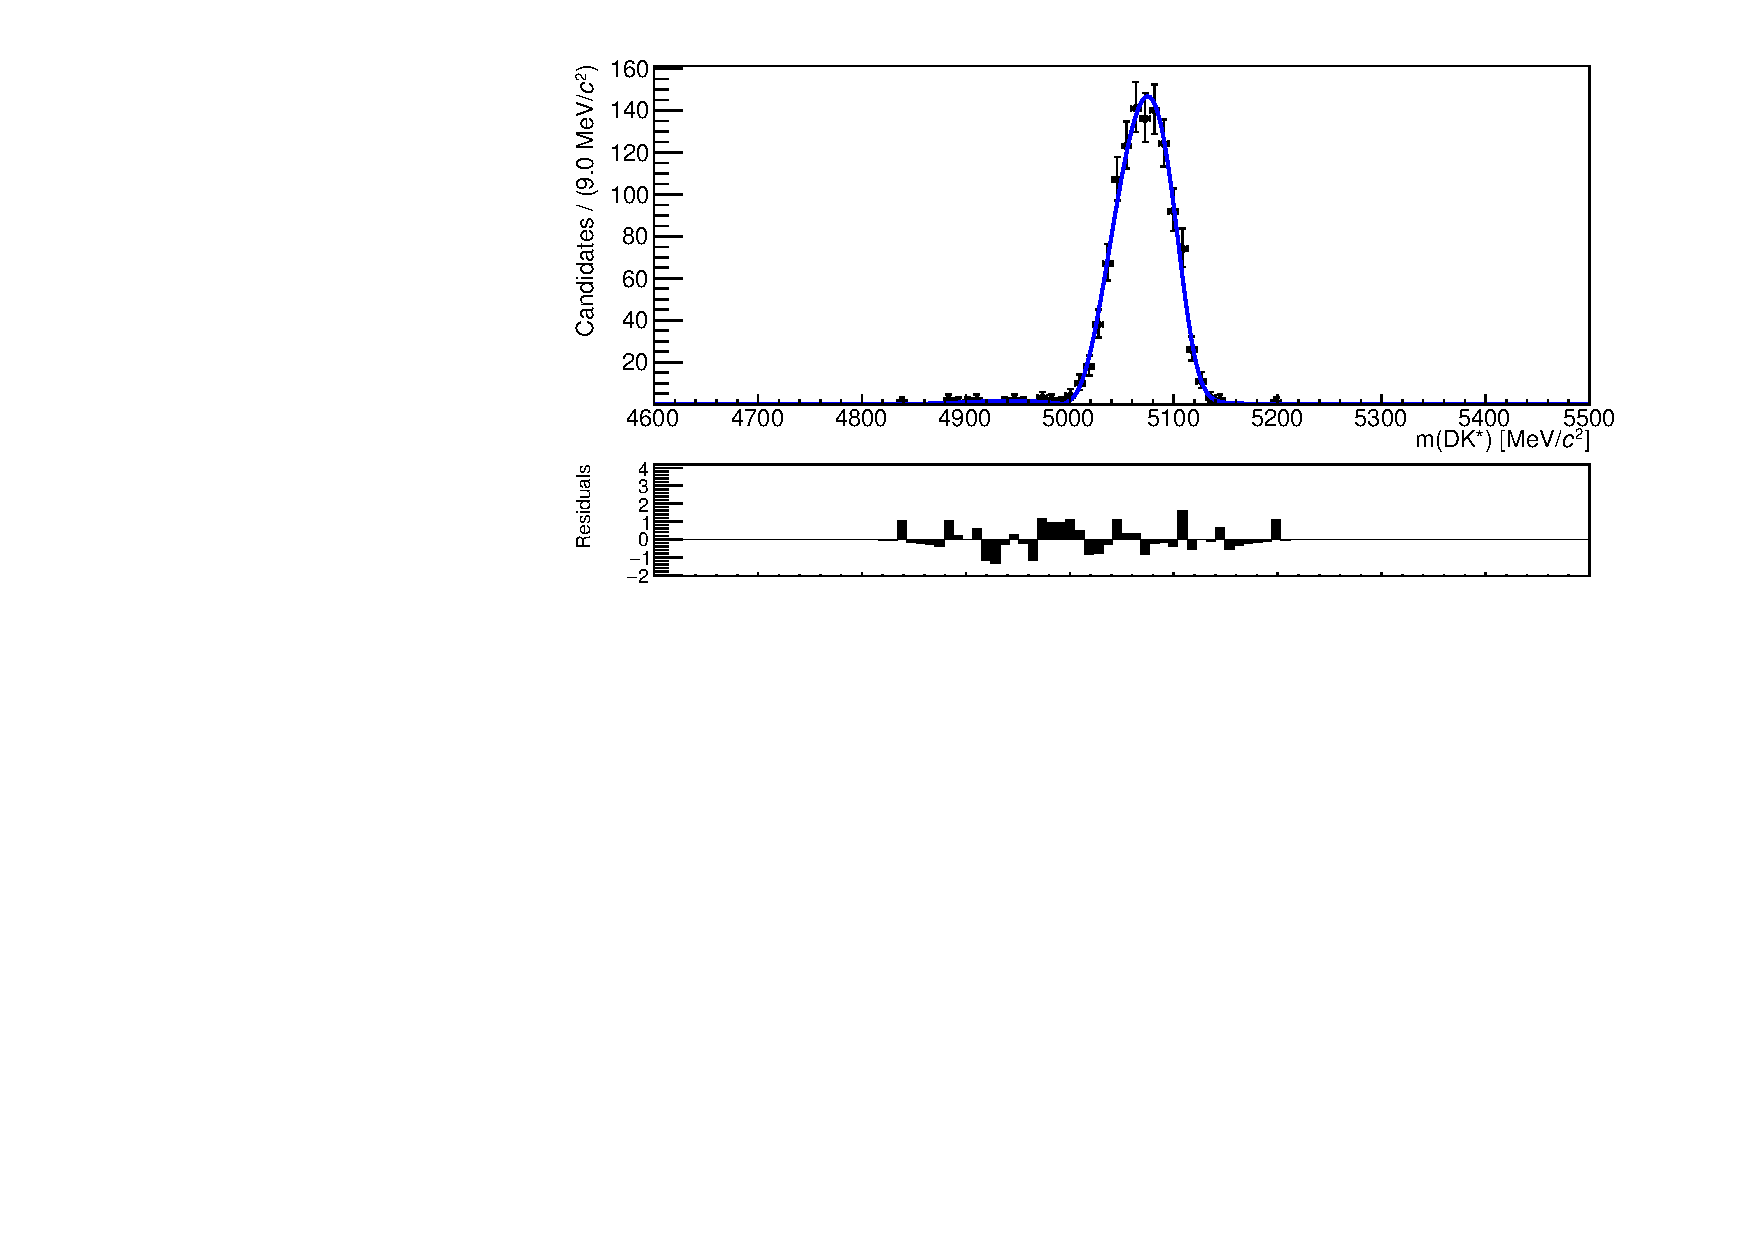
\includegraphics[width=0.5\linewidth]{figures/fitComponents/Bupi101_LL.pdf}
%\put(-170,70) {(b)}
%\hfill
%\includegraphics[width=0.5\linewidth]{figures/fitComponents/Bugamma010_LL.pdf}
%\put(-170,70) {(c)}
%\includegraphics[width=0.5\linewidth]{figures/fitComponents/Bugamma101_LL.pdf}
%\put(-170,70) {(d)}
%\hfill
%\includegraphics[width=0.5\linewidth]{figures/fitComponents/Bdpi010_LL.pdf}
%\put(-170,70) {(e)}
%\includegraphics[width=0.5\linewidth]{figures/fitComponents/Bdpi101_LL.pdf}
%\put(-170,70) {(f)}
%\caption{Results of the unbinned maximum likelihood fits to the \Bm mass distribution for $B \to D^*K^*$ \runone simulated samples in all the different modes for LL candidates (a) \decay{\Bm}{(\decay{\Dstarz}{\Dz[\piz]})\Kstarm} 0, (b) \decay{\Bm}{(\decay{\Dstarz}{\Dz[\piz]})\Kstarm} $\pm$1, (c) \decay{\Bm}{(\decay{\Dstarz}{\Dz[\gamma]})\Kstarm} 0, (d) \decay{\Bm}{(\decay{\Dstarz}{\Dz[\gamma]})\Kstarm} $\pm$1, (e) \decay{\Bd}{(\decay{\Dstarp}{\Dz[\pip]})\Kstarm} 0, and (f) \decay{\Bd}{(\decay{\Dstarp}{\Dz[\pip]})\Kstarm} $\pm$1. The residuals are shown at the bottom of each plot.}
%\label{partrecofitsLL}
%\end{figure}

\begin{figure}[h]
\includegraphics[width=0.5\linewidth]{figures/fitComponents/Bupi010_DD.pdf}
\put(-170,70) {(a)}
\includegraphics[width=0.5\linewidth]{figures/fitComponents/Bupi101_DD.pdf}
\put(-170,70) {(b)}
\hfill
\includegraphics[width=0.5\linewidth]{figures/fitComponents/Bugamma010_DD.pdf}
\put(-170,70) {(c)}
\includegraphics[width=0.5\linewidth]{figures/fitComponents/Bugamma101_DD.pdf}
\put(-170,70) {(d)}
\hfill
\includegraphics[width=0.5\linewidth]{figures/fitComponents/Bdpi010_DD.pdf}
\put(-170,70) {(e)}
\includegraphics[width=0.5\linewidth]{figures/fitComponents/Bdpi101_DD.pdf}
\put(-170,70) {(f)}
\caption{Results of the unbinned maximum likelihood fits to the \Bm mass distribution for $B \to D^*K^*$ \runone simulated samples for DD candidates (a) \decay{\Bm}{(\decay{\Dstarz}{\Dz[\piz]})\Kstarm} 0, (b) \decay{\Bm}{(\decay{\Dstarz}{\Dz[\piz]})\Kstarm} $\pm$1, (c) \decay{\Bm}{(\decay{\Dstarz}{\Dz[\gamma]})\Kstarm} 0, (d) \decay{\Bm}{(\decay{\Dstarz}{\Dz[\gamma]})\Kstarm} $\pm$1, (e) \decay{\Bd}{(\decay{\Dstarp}{\Dz[\pip]})\Kstarm} 0, and (f) \decay{\Bd}{(\decay{\Dstarp}{\Dz[\pip]})\Kstarm} $\pm$1. The residuals are shown at the bottom of each plot.}
\label{partrecofitsDD}
\end{figure}

As the shapes all occur in the same region of \Bm mass, allowing the six individual yield parameters to vary leads to an unstable fit. Therefore, it is necessary to apply additional constraints, in the form of fixing ratios of different yields. 

The total partially reconstructed PDF, $P_{partreco}$, is given by
\begin{equation}
P_{partreco} = f_0P_0 + (1 - f_0)P_{\pm 1}
\label{partrecofunction}
\end{equation}
where $P_0$ and $P_{\pm 1}$ represent the shapes for the \Dstar helicity states 0 and $\pm$1 respectively, and are given by
\begin{align*}
P_0 &= \frac{1}{1 + c^{\Bm,\gamma}_0 + c^{\Bd,\pi}_0} \left( P^{\Bm,\pi}_0 + c^{\Bm,\gamma}_0P^{\Bm,\gamma}_0 + c^{\Bd,\pi}_0P^{\Bd,\pi}_0 \right) \text{ ,} \\
P_{\pm 1} &= \frac{1}{1 + c^{\Bm,\gamma}_{\pm 1} + c^{\Bd,\pi}_{\pm 1}} \left( P^{\Bm,\pi}_{\pm 1} + c^{\Bm,\gamma}_{\pm 1}P^{\Bm,\gamma}_{\pm 1} + c^{\Bd,\pi}_{\pm 1}P^{\Bd,\pi}_{\pm 1} \right) \text{ .}
\end{align*}
Here $P_x^{y,z}$ represents the partially reconstructed PDF, where $x$ is the \Dstar helicity state ($0$ or $\pm 1$), $y$ is the type of \B meson (\Bm or \Bd), and $z$ is the particle missed in the reconstruction (\pion or \Pgamma). Similarly, $c_x^{y,z}$ are the ratios between the yields. The yield ratios between \decay{\Bm}{(\decay{\Dstarz}{\Dz[\piz]})\Kstarm}, \decay{\Bm}{(\decay{\Dstarz}{\Dz[\gamma]})\Kstarm} and \decay{\Bd}{(\decay{\Dstarp}{\Dz[\pip]})\Kstarm} are fixed separately for the 0 and $\pm$1 helicity states of the \Dstar. The expected yield ratios, $c^{\Bm,\gamma}_0$, $c^{\Bd,\pi}_0$, $c^{\Bm,\gamma}_{\pm 1}$ and $c^{\Bd,\pi}_{\pm 1}$ can be individually calculated from knowledge of the ratio of production of the relevant decays and the ratio of the efficiencies, detailed in \sect\ref{sec:selection} By way of example, 
\begin{align}
c^{\Bm,\gamma}_0 &= \frac{N(\decay{\Bm}{(\decay{\Dstarz}{\Dz\gamma})\Kstarm}\ 0)}{N(\decay{\Bm}{(\decay{\Dstarz}{\Dz\piz})\Kstarm}\ 0)} \nonumber \\ 
&= \frac{\mathcal{B}(\decay{\Bm}{(\decay{\Dstarz}{\Dz\gamma})\Kstarm}\ 0)}{\mathcal{B}(\decay{\Bm}{(\decay{\Dstarz}{\Dz\piz})\Kstarm}\ 0)} \times \frac{\epsilon_{sel}(\decay{\Bm}{(\decay{\Dstarz}{\Dz\gamma})\Kstarm}\ 0)}{\epsilon_{sel}(\decay{\Bm}{(\decay{\Dstarz}{\Dz\piz})\Kstarm}\ 0)}
\label{partrecoexample}
\end{align}
where $N$ represents the yield, $\mathcal{B}$ represents the branching fraction and $\epsilon_{sel}$ represents the selection efficiency of the partially reconstructed decay. The branching fractions using in the ratios are given in \tab\ref{partrecoBRs}. The selection efficiency, $\epsilon_{sel}$, calculated using simulated samples, is defined as the number of partially reconstructed events passing the selection compared to the number generated. Using \eqn\ref{partrecoexample} and equivalent calculations, the values are then fixed in the mass fit. The estimated yield ratios are given in \tab\ref{fixedyieldratios}. 

\begin{table}[h]
\centering
\begin{tabular}{c|c}
Mode & Branching ratio \\
\hline
\decay{\Bm}{(\decay{\Dstarz}{\Dz\piz})\Kstarm} & $(5.0 \pm 0.9) \times 10^{-4}$ \\
\decay{\Bm}{(\decay{\Dstarz}{\Dz\gamma})\Kstarm} & $(3.1 \pm 0.6) \times 10^{-4}$ \\
\decay{\Bd}{(\decay{\Dstarp}{\Dz\pip})\Kstarm} & $(2.2 \pm 0.4) \times 10^{-4}$ \\
\end{tabular}
\caption{Branching ratios for the different partially reconstructed decay modes. These are taken from Ref~\cite{PDG2016}, constructed by multiplying the relevant \B and \Dstar branching fractions.}
\label{partrecoBRs}
\end{table}

\begin{table}[h]
\centering
\begin{tabular}{ccc}
\hline
& LL & DD \\
\hline
$c^{\Bm,\gamma}_0$ & $0.53 \pm 0.14$ & $0.51 \pm 0.14$ \\[3mm]
$c^{\Bd,\pi}_0$ & $0.38 \pm 0.14$ & $0.37 \pm 0.14$ \\[3mm]
$c^{\Bm,\gamma}_{\pm 1}$ & $0.53 \pm 0.14$ & $0.51 \pm 0.14$ \\[3mm]
$c^{\Bd,\pi}_{\pm 1}$ & $0.38 \pm 0.14$ & $0.38 \pm 0.14$ \\[3mm]
\hline
\end{tabular}
\caption{Yield ratios fixed in the mass fit for the partially reconstructed backgrounds.}
\label{fixedyieldratios}
\end{table}

Other backgrounds investigated in this analysis, but not included in the mass fit, are discussed in \sect\ref{sec:backgrounds}.


\subsection{Mass fit to the data in the favoured modes}
\label{sec:massfit:fit}

Extended maximum likelihood fits to the invariant B mass in the \kpi and \kpipipi favoured modes are performed using the shapes discussed in Secs.~\ref{sec:massfit:signal}, \ref{sec:massfit:combinatorial} and \ref{sec:massfit:partreco}. The total extended likelihood PDFs used to model the data are given by
\begin{equation}
P_{tot}(x_i;\mathbb{O}, N) = N_{sig}P_{sig} + N_{comb}P_{comb} + N_{partreco}P_{partreco} \text{ ,}
\label{totalpdf}
\end{equation}
where $x_i$ is the reconstructed \Bm mass of the candidate and $\mathbb{O}$ are the set of parameters to be optimised, namely $\{\mu, \sigma, \beta, f_0\}$, along with the expected yields, $N$, of the signal, combinatorial and partially reconstructed PDFs, $\{N_{sig}, N_{comb}, N_{partreco}\}$, as additional freely varying parameters to be determined, as described in \sect\ref{sec:massfit:likelihood}. The signal PDF, $P_{sig}$, is given by \eqn\ref{DCBshape}, the combinatorial PDF, $P_{comb}$, is given by \eqn\ref{combpdf}, where the slope parameter $\beta$ varies in the fit, and the partially reconstructed PDF, $P_{partreco}$, is given by \eqn\ref{partrecofunction}. The yield of the signal and combinatorial PDFs, $N_{sig}$ and $N_{comb}$, are left to vary without constraint, as well as the peak position, $\mu$, and width, $\sigma$, of the signal PDF. The only parameters not fixed in the partially reconstructed background are the yield ratio between the 0 and $\pm$1 amplitudes, $f_0$, and the overall yield, $N_{partreco}$.

Figures~\ref{massfitskpi} and \ref{massfitsk3pi} show the results of the extended maximum likelihood fits to the invariant B mass distribution in the \kpi and \kpipipi favoured modes respectively, for LL and DD candidates in both Run 1 and Run 2. The estimated signal yields extracted from these fits are given in \tab\ref{signalyields}. It can be seen that the yield in the \kpi mode is almost twice as large as that in the \kpipipi mode, which is primarily a result of the lower reconstruction efficiency due to the two additional tracks in the four-body mode, and additional PID requirements necessary to reduce faking backgrounds. \Tab\ref{signalyields} also shows that the yield per unit of integrated luminosity is about 3 times higher in \runone (3~\invfb) compared to \runtwo (1.8~\invfb), which is driven by the increase in centre-of-mass energy in \runtwo. The gain in yield between Run 1 and Run 2 is not the same for the two- and four-body modes due to the difference in trigger efficiencies.

The results for the \kpi and \kpipipi fits are shown in Tables~\ref{fitresultskpi} and \ref{fitresultsk3pi} respectively. The values of $\mu$ are all consistent with the known \Bm mass of 5279.3\mevcc. The slight variations in the values are primarily due to the statistical uncertainty in the data. The widths of the signal shape are found to be smaller in the LL samples compared to the DD samples, which is expected as the resolution is better when forming a vertex from long tracks. The parameter $f_0$ is the yield ratio between 0 and $\pm$1 helicity amplitudes in the partially reconstructed background, which is purely dependent on the physics of the decay, so should not vary depending on the data sample used. As observed in data, $f_0$ is found to be consistent between all of the categories in the \kpi and \kpipipi mass fits separately.

\begin{table}
\centering
\begin{tabular}{l|cc|cc}
\hline
& \multicolumn{2}{c}{\kpi} & \multicolumn{2}{c}{\kpipipi} \\
& \runone & \runtwo & \runone & \runtwo \\
\hline
LL & $220 \pm 16$ & $388 \pm 21$ & $87 \pm 10$ & $215 \pm 15$ \\
DD & $505 \pm 24$ & $901 \pm 33$ & $205 \pm 16$ & $516 \pm 25$ \\
\hline
\end{tabular}
\caption{Signal yields from the \kpi and \kpipipi mass fits for both \KS reconstruction types and data-taking periods separately.}
\label{signalyields}
\end{table}

\begin{figure}
\centering
\includegraphics[width=0.78\linewidth]{figures/fitComponents/massFit_LL_KPi_run1.pdf}
\put(-280,120) {(a)}
\hfill
\includegraphics[width=0.78\linewidth]{figures/fitComponents/massFit_DD_KPi_run1.pdf}
\put(-280,120) {(b)}
\hfill
\includegraphics[width=0.78\linewidth]{figures/fitComponents/massFit_LL_KPi_run2.pdf}
\put(-280,120) {(c)}
\hfill
\includegraphics[width=0.78\linewidth]{figures/fitComponents/massFit_DD_KPi_run2.pdf}
\put(-280,120) {(d)}
\caption{Results of the unbinned maximum likelihood fits to the \kpi invariant B mass distribution for (a) \runone LL, (b) \runone DD, (c) \runtwo LL, and (d) \runtwo DD. The black points represent the data, while the blue curve is the projection of the optimised shape of the form given in \eqn\ref{totalpdf}.}
\label{massfitskpi}
\end{figure}

\begin{figure}
\centering
\includegraphics[width=0.78\linewidth]{figures/fitComponents/massFit_LL_KPiPiPi_run1.pdf}
\put(-280,120) {(a)}
\hfill
\includegraphics[width=0.78\linewidth]{figures/fitComponents/massFit_DD_KPiPiPi_run1.pdf}
\put(-280,120) {(b)}
\hfill
\includegraphics[width=0.78\linewidth]{figures/fitComponents/massFit_LL_KPiPiPi_run2.pdf}
\put(-280,120) {(c)}
\hfill
\includegraphics[width=0.78\linewidth]{figures/fitComponents/massFit_DD_KPiPiPi_run2.pdf}
\put(-280,120) {(d)}
\caption{Results of the unbinned maximum likelihood fits to the \kpipipi invariant B mass distribution for (a) \runone LL, (b) \runone DD, (c) \runtwo LL, and (d) \runtwo DD. The black points represent the data, while the blue curve is the projection of the optimised shape of the form given in \eqn\ref{totalpdf}.}
\label{massfitsk3pi}
\end{figure}

\begin{table}[h]
\centering
\subfloat[Fit results from the \kpi favoured mode.][Fit results from the \kpi favoured mode.]{
\resizebox{\textwidth}{!}{
\begin{tabular}{l|cc|cc}
\hline
& \multicolumn{2}{c}{Run 1} & \multicolumn{2}{c}{Run 2} \\
& LL & DD & LL & DD \\
\hline
$\beta/\mevcc^{-1}$ & $(-4.8 \pm 0.5) \times 10^{-3}$ & $(-2.8 \pm 0.3) \times 10^{-3}$ & $(-4.4 \pm 0.5) \times 10^{-3}$ & $(-2.5 \pm 0.2) \times 10^{-3}$ \\
$f_0$ & $0.15 \pm 0.08$ & $0.12 \pm 0.05$ & $0.18 \pm 0.05$ & $0.06 \pm 0.04$ \\
$\mu/\mevcc$ & $5280.7 \pm 0.8$ & $5280.7 \pm 0.6$ & $5278.5 \pm 0.8$ & $5278.6 \pm 0.5$ \\
$N_{comb}$ & $167 \pm 20$ & $472 \pm 34$ & $223 \pm 24$ & $1100 \pm 50$ \\
$N_{partreco}$ & $338 \pm 23$ & $810 \pm 36$ & $654 \pm 31$ & $1397 \pm 49$ \\
$N_{sig}$ & $220 \pm 16$ & $505 \pm 24$ & $388 \pm 21$ & $901 \pm 33$ \\
$\sigma/\mevcc$ & $10.2 \pm 0.7$ & $11.5 \pm 0.5$ & $12.2 \pm 0.6$ & $11.5 \pm 0.4$ \\
\hline
\end{tabular}}
\label{fitresultskpi}}
\hfill
\subfloat[Fit results from the \kpipipi favoured mode.][Fit results from the \kpipipi favoured mode.]{
\resizebox{\textwidth}{!}{
\begin{tabular}{l|cc|cc}
\hline
& \multicolumn{2}{c}{Run 1} & \multicolumn{2}{c}{Run 2} \\
& LL & DD & LL & DD \\
\hline
$\beta/\mevcc^{-1}$ & $(-5.2 \pm 1.1) \times 10^{-3}$ & $(-2.3 \pm 0.4) \times 10^{-3}$ & $(-4.4 \pm 0.5) \times 10^{-3}$ & $(-2.1 \pm 0.2) \times 10^{-3}$ \\
$f_0$ & $0.26 \pm 0.11$ & $0.20 \pm 0.08$ & $0.15 \pm 0.07$ & $0.16 \pm 0.05$ \\
$\mu/\mevcc$ & $5281.3 \pm 1.3$ & $5283.9 \pm 0.9$ & $5278.7 \pm 1.0$ & $5277.7 \pm 0.7$ \\
$N_{comb}$ & $50 \pm 12$ & $252 \pm 24$ & $168 \pm 20$ & $707 \pm 40$ \\
$N_{partreco}$ & $154 \pm 15$ & $317 \pm 24$ & $342 \pm 23$ & $914 \pm 40$ \\
$N_{sig}$ & $102 \pm 10$ & $226 \pm 16$ & $244 \pm 16$ & $578 \pm 27$ \\
$\sigma/\mevcc$ & $11.4 \pm 1.0$ & $11.3 \pm 0.8$ & $12.9 \pm 0.8$ & $13.1 \pm 0.6$ \\
\hline
\end{tabular}}
\label{fitresultsk3pi}}
\caption{Fit results from the \kpi and \kpipipi favoured modes, corresponding to the fits in \figs\ref{massfitskpi} and \ref{massfitsk3pi}. The parameter $\beta$ is the combinatorial background slope, $f_0$ is the yield ratio between 0 and $\pm$1 helicity amplitudes, $\mu$ and $\sigma$ are the peak position and width of the signal shape, and $N_{sig}$, $N_{comb}$ and $N_{partreco}$ are the yields of signal, combinatorial background and partially reconstructed decays respectively.}
\end{table}


\clearpage
